%%%---PREAMBLE---%%%%%%%%%%%%%%%%%%%%%%%%%%%%
\documentclass[oneside,12pt,final]{sty/ucthesis-CA2012}
\pdfoutput=1

%--- Packages ---------------------------------------------------------
\usepackage[lofdepth,lotdepth,caption=false]{subfig}
\usepackage{fancyhdr}
\usepackage[hidelinks,pdfencoding=auto,psdextra]{hyperref}
\usepackage{amsmath, amssymb, slashed, graphicx}
\usepackage{xspace}
\usepackage{braket}
\usepackage{color}
\usepackage{setspace}
\usepackage{cite}
\usepackage{multirow}
\usepackage{nicefrac}
\usepackage{feynmp-auto}
\unitlength = 1mm
%\usepackage{subfigure} (Subfigure package clashes with another package)

%---New Definitions and Commands------------------------------------------------------
\def\half{\frac{1}{2}}
\newcommand{\be}{\begin{equation}}
\newcommand{\ee}{\end{equation}}
\newcommand{\mbb}[1]{\mathbb{#1}}
\newcommand{\mrm}[1]{\mathrm{#1}}
\newcommand{\mcal}[1]{\mathcal{#1}}
\newcommand{\mbf}[1]{\mathbf{#1}}
\newcommand{\ph}[1]{\phantom{#1}}
\newcommand{\sthirteen}{\ensuremath{\sqrt{\mathrm{s}}=13~\mathrm{TeV}}\xspace}
\newcommand{\ifb}{fb\ensuremath{{}^{-1}}}
\newcommand{\rs}{R\&S\xspace}
\newcommand{\pt}{\ensuremath{p_\mrm{T}}\xspace}
\newcommand{\vpt}{\ensuremath{\vec{p}_{\> \mathrm{T}}}\xspace}
\newcommand{\ptmiss}{\ensuremath{\pt^\mrm{miss}}\xspace}
\newcommand{\ptireco}{\ensuremath{p_{\mrm{T},i}^\mrm{reco}}\xspace}
\newcommand{\ptireb}{\ensuremath{p_{\mrm{T},i}^\mrm{reb}}\xspace}
\newcommand{\mttwo}{\ensuremath{M_{\mrm{T2}}}\xspace}
\newcommand{\Ht}{\ensuremath{H_{\mrm{T}}}\xspace}
\newcommand{\Met}{\ptmiss}
\newcommand{\Mht}{\ensuremath{H_{\mrm{T}}^{\mrm{miss}}}\xspace}
\newcommand{\vSS}[3]{\ensuremath{\vec{#1}_{\> #2}^{\> #3}}}
\newcommand{\vMet}{\ensuremath{\vec{p}_{\> \mathrm{T}}^{\> \mathrm{miss}}}\xspace}
\newcommand{\vMht}{\ensuremath{\vec{H}_{\mrm{T}}^{\mrm{miss}}}\xspace}
\newcommand{\dpmin}{\ensuremath{\Delta\phi_{\mrm{min}}}\xspace}
\newcommand{\dphimet}{\ensuremath{\Delta\phi(\mathrm{j}_{1234},\vMet)}\xspace}
\newcommand{\njets}{\ensuremath{N_{\mrm{j}}}\xspace}
\newcommand{\nbtags}{\ensuremath{N_\mrm{b}}\xspace}
\newcommand{\Nj}{\njets}
\newcommand{\Nb}{\nbtags}
\newcommand{\Mt}{\ensuremath{M_{\mrm{T}}}\xspace}
\newcommand{\wjets}{\ensuremath{W\mrm{+jets}}\xspace}
\newcommand{\zjets}{\ensuremath{Z\mrm{+jets}}\xspace}
\newcommand{\vjets}{\ensuremath{\mrm{V}\mrm{+jets}} \ensuremath{(\mrm{V}=Z,W)}\xspace}
\newcommand{\ttbar}{\ensuremath{t\bar{t}}\xspace}
\newcommand{\qqbar}{\ensuremath{q\bar{q}}\xspace}
\newcommand{\qqbarpr}{\ensuremath{q\bar{q}'}\xspace}
\newcommand{\ttjets}{\ensuremath{\ttbar \mrm{+jets}}\xspace}
\newcommand{\ttV}{\ensuremath{\ttbar\mrm{V} (\mrm{V}=Z,W)}\xspace}
\newcommand{\znunu}{\ensuremath{Z\to\nu\bar{\nu}}\xspace}
\newcommand{\zll}{\ensuremath{Z\to\ell^+\ell^-}\xspace}
\newcommand{\ptj}{\ensuremath{\pt^{\mrm{jet}}}\xspace}
\newcommand{\gluino}{\ensuremath{{\widetilde{g}}}\xspace}
\newcommand{\lsp}{\ensuremath{{\widetilde{\chi}_1^0}}\xspace}
\newcommand{\Lint}{137 fb$^{-1}$}
\newcommand{\chizz}{\ensuremath{\widetilde{\chi}_2^0}\xspace}
\newcommand{\chargino}{\ensuremath{\widetilde{\chi}_1^\pm}\xspace}
\newcommand{\charginoplus}{\ensuremath{\widetilde{\chi}_1^+}\xspace}
\newcommand{\charginominus}{\ensuremath{\widetilde{\chi}_1^-}\xspace}
\newcommand{\SQu}{\ensuremath{\widetilde{u}}\xspace}
\newcommand{\SQd}{\ensuremath{\widetilde{d}}\xspace}
\newcommand{\SQs}{\ensuremath{\widetilde{s}}\xspace}
\newcommand{\SQc}{\ensuremath{\widetilde{c}}\xspace}
\newcommand{\SQb}{\ensuremath{\widetilde{b}}\xspace}
\newcommand{\SQt}{\ensuremath{\widetilde{t}}\xspace}
\newcommand{\SQq}{\ensuremath{\widetilde{q}}\xspace}
\newcommand{\SQqL}{\ensuremath{\widetilde{q}_\mrm{L}}\xspace}
\newcommand{\SQqR}{\ensuremath{\widetilde{q}_\mrm{R}}\xspace}
\newcommand{\lqs}{\ensuremath{\text{LQ}_\text{S}}\xspace}
\newcommand{\lqv}{\ensuremath{\text{LQ}_\text{V}}\xspace}


\newcommand{\MeV}{\ensuremath{\;\text{Me\hspace{-.08em}V}}\xspace}
\newcommand{\GeV}{\ensuremath{\;\text{Ge\hspace{-.08em}V}}\xspace}
\newcommand{\TeV}{\ensuremath{\;\text{Te\hspace{-.08em}V}}\xspace}

% \def\dsp{\def\baselinestretch{1.0}\large\normalsize} % FIXME remove this line when compiling final thesis
% https://stackoverflow.com/questions/1465665/passing-command-line-arguments-to-latex-document/1466610#1466610
\ifdefined\myownflag
    \def\dsp{\def\baselinestretch{1.0}\large\normalsize} % FIXME remove this line when compiling final thesis
\fi

%---Set Margins ------------------------------------------------------
\setlength\oddsidemargin{0.25 in} \setlength\evensidemargin{0.25 in} \setlength\textwidth{6.25 in} \setlength\textheight{8.50 in}
\setlength\footskip{0.25 in} \setlength\topmargin{0 in} \setlength\headheight{0.25 in} \setlength\headsep{0.25 in}

%%%---DOCUMENT---%%%%%%%%%%%%%%%%%%%%%%%%%%%%
\begin{document}


%=== Preliminary Pages ============================================
\begin{frontmatter}
	%%%%%%%%%%%%%%%%%%%%%%%%%%%
% TITLE PAGE INFORMATION %
%%%%%%%%%%%%%%%%%%%%%%%%%%%


\title{
Search for new physics using the $\text{M}_\text{T2}$ variable in all-hadronic final states 
produced in 13 TeV proton-proton collisions with the CMS detector
}

\author{Bennett J. Marsh}

%%%%%%%%%%%%%%%%%%%%%%%%%%%%%%%%%%
% DECLARATIONS FOR FRONT MATTER %
%%%%%%%%%%%%%%%%%%%%%%%%%%%%%%%%%%
\report{Dissertation} \degree{Doctor of Philosophy} 
\degreemonth{July} 
\degreeyear{2019}
\defensemonth{July} % should be one of the following: March, 
\defenseyear{2019}

\chair{Professor Claudio Campagnari}  % this is your advisor
\othermemberA{Professor David Stuart} % This is a member of your committee 
\othermemberB{Professor Nathaniel Craig} % This is a member of your committee 
%% \othermemberC{Professor Jackmerius Tacktheritrix} % This is a member of your committee (if your department requires 4 members)
\numberofmembers{3} % should match the number of entries above (chair + othermembers)

\field{Physics}
\campus{Santa Barbara}

	\maketitle
	\approvalpage
	\copyrightpage
	% \begin{dedication}

\bigskip

${}$ \\

\bigskip

${}$ \\

\bigskip

${}$ \\

\bigskip

\begin{center}
\begin{Large}
Dedication here
\end{Large}
\end{center}


\end{dedication} %comment out if you don't want a dedication
	\begin{acknowledgements}

Acknowledgments here.

\end{acknowledgements} 

	\begin{vitae}
\addcontentsline{toc}{chapter}{Curriculum Vitae}

\begin{vitaesection}{Education}
\vspace{-0.1cm}
\item [2020] Ph.D. in Physics, University of California, Santa Barbara.
\item [2018] M.A. in Physics, University of California, Santa Barbara.
\item [2015] B.S. in Physics and Mathematics, Purdue University, West Lafayette, IN.
\end{vitaesection}

\vspace{0.5cm}
\textbf{Publications}

%% \nobibliography*
%% \begin{itemize}
    %% \item \bibentry{GAN:LHC2019} % http://inspirehep.net/record/1714018
    %% \item \bibentry{CMS:myTOPRun2PAS} % http://inspirehep.net/record/1726177
    %% \item \bibentry{CMS:mySUSRun2PAS} % http://inspirehep.net/record/1726691
    %% \item \bibentry{CMS:myTOP2016} % http://inspirehep.net/record/1633423
    %% \item \bibentry{CMS:mySUS2016} % http://inspirehep.net/record/1594731
%% \end{itemize}

\begin{itemize}

\item CMS Collaboration, ``Searches for physics beyond the standard model with the $M_\mathrm{T2}$ variable in hadronic
  final states with and without disappearing tracks in proton-proton collisions at $\sqrt{s}=13~\mathrm{TeV}$.''
  \textit{Eur. Phys. J. C} \textbf{80} (2020), 3.
  [\href{https://arxiv.org/abs/1909.03460}{arXiv:1909.03460}].

\item CMS Collaboration, ``Constraints on models of scalar and vector leptoquarks decaying to a quark
  and a neutrino at $\sqrt{s}=13~\mathrm{TeV}$.'' \textit{Phys. Rev. D}
  \textbf{98} (2018), 032005. 
  [\href{https://arxiv.org/abs/1805.10228}{arXiv:1805.10228}].

\item CMS Collaboration, ``Search for new phenomena with the $M_\mathrm{T2}$ variable in the all-hadronic
  final state produced in proton-proton collisions at $\sqrt{s}=13~\mathrm{TeV}$.'' \textit{Eur. Phys J. C}
  \textbf{77} (2017), 710.
  [\href{https://arxiv.org/abs/1705.04650}{arXiv:1705.04650}].

\item A. Ball \textit{et al}. ``A Letter of Intent to Install a Milli-Charged Particle Detector at LHC P5.'' July 2016.
  [\href{https://arxiv.org/abs/1607.04669}{arXiv:1607.04669}].

\end{itemize}


\vspace{0.2cm}
\textbf{Public Talks}

\begin{itemize}

\item ``The milliQan experiment: a search for milli-charged particles at the LHC''.
Light Dark Matter @ Accelerators Workshop, Nov. 20--22, 2019. Venice, Italy.

\item ``Monitoring tools for the muon system in the Compact Muon Solenoid (CMS) detector''.
Machine Learning in Science and Engineering Conference, June 6--8, 2018. Carnegie Mellon
University, Pittsburgh, PA.

\end{itemize}

\end{vitae}

	\begin{abstract}
\addcontentsline{toc}{chapter}{Abstract}

A search for phenomena beyond the Standard Model (BSM) is performed using events with 
hadronic jets and significant transverse momentum imbalance. The results are based on 
a sample of proton-proton collisions at a center-of-mass energy of $13\TeV$, collected 
by the CMS experiment at the Large Hadron Collider in 2016--2018 and corresponding to an integrated luminosity 
of \Lint. The search is based on signal regions defined by the hadronic 
energy in the event, the jet multiplicity, the number of b-tagged jets, 
and the value of the kinematic variable \mttwo for events with at least 
two jets. For events with exactly one jet, the transverse momentum of the jet is used 
instead. No significant excess event yield is observed above the predicted Standard Model background. This is used 
to constrain a range of BSM models that predict the following: the pair production of gluinos 
and squarks in the context of supersymmetry models conserving $R$-parity; the resonant production of a 
colored scalar state decaying to a massive Dirac fermion and a quark; and the pair production 
of scalar and vector leptoquarks each decaying to a neutrino and a top, bottom, or 
light-flavor quark. In most of the cases, the results obtained are the most stringent 
constraints to date.

%\abstractsignature
\end{abstract}



	\tableofcontents
\end{frontmatter}

\begin{mainmatter}

%---Set Headers and Footers ------------------------------------------------------
\pagestyle{fancy}
\renewcommand{\chaptermark}[1]{\markboth{{\sf #1 \hspace*{\fill} Chapter~\thechapter}}{} }
\renewcommand{\sectionmark}[1]{\markright{ {\sf Section~\thesection \hspace*{\fill} #1 }}}
\fancyhf{}

\makeatletter \if@twoside \fancyhead[LO]{\small \rightmark} \fancyhead[RE]{\small\leftmark} \else \fancyhead[LO]{\small\leftmark}
\fancyhead[RE]{\small\rightmark} \fi

\def\cleardoublepage{\clearpage\if@openright \ifodd\c@page\else
  \hbox{}
  \vspace*{\fill}
  \begin{center}
    This page intentionally left blank
  \end{center}
  \vspace{\fill}
  \thispagestyle{plain}
  \newpage
  \fi \fi}
\makeatother
\fancyfoot[c]{\textrm{\textup{\thepage}}} % page number
\fancyfoot[C]{\thepage}
\renewcommand{\headrulewidth}{0.4pt}

\fancypagestyle{plain} { \fancyhf{} \fancyfoot[C]{\thepage}
\renewcommand{\headrulewidth}{0pt}
\renewcommand{\footrulewidth}{0pt}}

%\chapter{Introduction}

\begin{section}{Info}
Some facts

\begin{itemize}

\item Standard model missing some stuff
\item LHC smashes protons together very fast
\item CMS detector is very big
\item Analyze CMS data to find stuff beyond the standard model (e.g., SUZY)
\item Did not find anything

\end{itemize}

%The results presented in this thesis correspond to the published results in Refs.~\cite{CMS:myTOPRun2PAS,CMS:mySUSRun2PAS,CMS:myTOP2016,CMS:mySUS2016}

\end{section}

\chapter{The Standard Model and Beyond}
\label{chap:theory}

The Standard Model of particle physics describes all
known fundemental particles and the interactions between them (with the exception
of the gravitational force). Developed over decades in the latter half of the 20$^\mrm{th}$
century, it has predicted experimental findings to an extraordinary degree of accuracy,
and represents one of the crowning achievements of modern science.
However, despite it successes, there are a number of known phenomena that cannot be
explained with the current theory, giving physicists reason to look for an expanded model.
In this chapter, we outline the Standard Model as it currently exists, discuss some
of the challenges that the model faces, and give a brief survey of proposed extensions to
the Standard Model that are relevant to this thesis.


\section{The Standard Model of particle physics}

The Standard Model (SM) is at its core a quantum field theory defined by a local 
$SU(3)\times SU(2)_L\times U(1)$ gauge symmetry. We will explain what exactly this means shortly 
(basically, each term gives rise to one of the three fundamental interactions), but for now we simply
describe all of the known particles and their properties.

\begin{figure}[ht]
  \begin{center}
    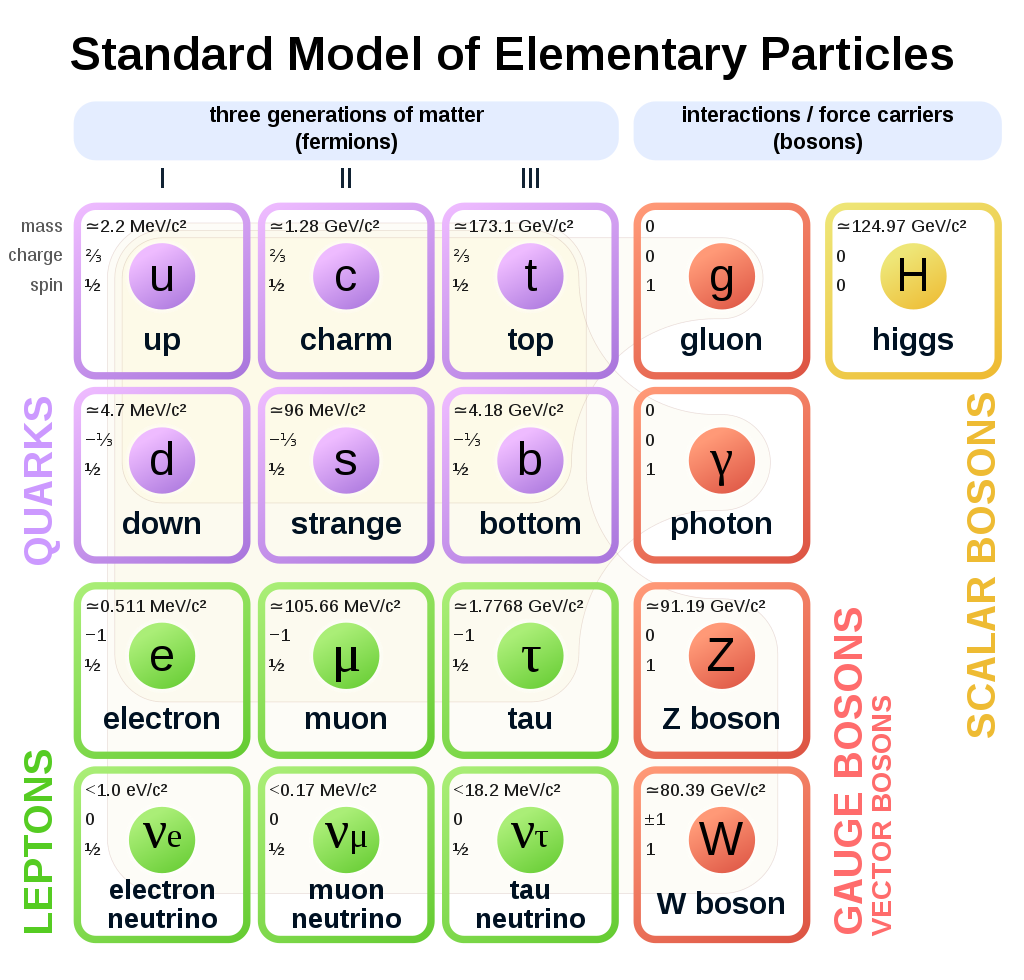
\includegraphics[width=0.70\textwidth]{figs/theory/standard_model.png}
    \caption{Diagram of all fundemental particles making up the Standard Model. There are 12 fermions (spin-\nicefrac{1}{2}), 
      consisting of six quarks (purple) and six leptons (green), 
      and divided into three generations. There are additionally four force-carrying vector bosons (spin-1),
      that couple to the fermions and give rise to the strong, weak, and electromagnetic interactions.
      Finally, the scalar Higgs boson, proposed in 1964 and discovered in 2012, provides the mechanism
      by which the other particles acquire mass. (Taken from \cite{SM_diagram})
            }
    \label{fig:sm}
  \end{center}
\end{figure}

\subsection{Fundamental particles}

Figure~\ref{fig:sm} shows all distinct particles in the SM, organized into groups.
On the left, in purple and green, are the 12 fundamental fermions, defined by the
value of their intrinsic angular momentum, or ``spin'', of \nicefrac{1}{2} (in units
of $\hbar$). By the spin-statistics theorem, fermions obey the Pauli exclusion principle,
meaning no two can occupy the same quantum state simultaneously.

The fermions are further defined by the various charges they carry (which determine how they
interact with the bosons, as we will see). In green are the six leptons, three with electric charge
of $-1$ (electron, muon and tau) and three that are electrically neutral (electron neutrino, muon
neutrino, and tau neutrino). In purple are the 6 types of quarks. The up-type quarks (up, charm, and top)
have electric charges of $+2/3$, and the down-type quarks (down, strange, and bottom) have electric
charges of $-1/3$. The quarks, in contrast to the leptons, carry color charge, meaning they
can interact via the strong interaction. All quarks and leptons carry weak isospin, meaning they can interact
via the weak interaction. Each of the fermions also has a corresponding antiparticle, which has the same
mass but opposite charges.

The fermions can be classified into three generations as indicated in the diagram, with masses
increasing in each generation. Due to various conservation laws arising from the allowed 
interactions, the first-generation particles are all stable, and hence form the building
blocks of matter. The strong interaction allows up and down quarks to strongly bind to
one another, forming protons (two ups and a down) and neutrons (two downs and an up).
The strong interaction further binds these into nuclei, which themselves bind to electrons via the electromagnetic
interaction to form atoms.

Moving to the right in the diagram, in red we have the four gauge bosons, which have spin-1
and which mediate the fundamental interactions. Their integer spin means they obey Bose statistics,
and are not constrained by the Pauli exclusion principle as are fermions. 
The gluon is massless, electrically neutral and mediates the strong
interaction. The photon is also massless and neutral and mediates the electromagnetic interaction. Finally,
the $W$ and $Z$ bosons are massive and mediate the weak interaction. The $Z$ is electrically neutral while 
the $W$ can carry charges of $\pm1$.

Finally, in yellow is the scalar (spin-0) Higgs boson. The Higgs mechanism was proposed in 1964 as an explanation
for how gauge bosons can acquire mass~\cite{Englert,Higgs,Guralnik}. A consquence of this mechanism is the prediction of a
scalar boson of undetermined mass, that couples to all SM particles proportionally to their masses.
The discovery of new boson of mass 125\GeV fitting these criteria (at least at the limits of current experimental precision) 
was announced by the CMS and ATLAS collaborations in July 2012~\cite{ATLAS:higgs,CMS:higgs}.

\subsection{Fundamental interactions}

Empirically, there are four known fundamental interactions, or ``forces'', between particles in our universe: 
the electromagnetic, weak, strong, and gravitational interactions. Gravity is understood
through Einstein's theory of general relativity, and is not (yet) integrated with our quantum understanding
of elementary particles. The other three interactions, on the other hand, are mathematically described by the
SM.

Essentially, each of the interactions arises by requiring that the Lagrangian describing the particle dynamics is
invariant under a certain \textit{local gauge transformation}. This means that if the particle fields are transformed
by some function that depends on spacetime position $x$, the Lagrangian is unchanged.
The full details are given in any quantum field theory textbook (e.g.~\cite{Peskin}), and we just give a brief
summary of the main ideas here.

The simplest example is the electromagnetic interaction. Starting with the Lagrangian of a free fermion
\be\label{eq:ferm_lagr}
\mathcal{L}_\mrm{fermion} = i\bar{\psi}\gamma^\mu\partial_\mu\psi - m\bar{\psi}\psi,
\ee
where $\psi$ is the spinor field of the fermion and $m$ is its mass,
we require that $\mathcal{L}$ is invariant under the local $U(1)$ transformation $\psi\to e^{-iq\theta(x)}\psi$.
The Lagrangian in Eq.~\ref{eq:ferm_lagr} is \textit{not} invariant under this transformation,
as we are left with an extra term proportional to $\partial_\mu\theta(x)$.

It turns out we can fix this by adding an extra term $-q\bar{\psi}\gamma^\mu\psi A_\mu$, where
$A_\mu$ is a new vector field that transforms by $A_\mu\to A_\mu+\partial_\mu\theta$. The new terms
introduced by the gauge transformation then cancel, and the Lagrangian is invariant.  The field
$A_\mu$ represents a new spin-1 particle, and to ensure that the Klein-Gordon equation is satisfied,
we must also add a ``free'' term. Doing this, it turns out the boson must be massless to ensure gauge invariance is
maintained.

So by requiring that the Lagrangian for a free fermion is invariant under a local $U(1)$ transformation,
we were forced to introduce a new massless, spin-1 boson that couples to the fermion via the term
$q\bar{\psi}\gamma^\mu\psi A_\mu$. This new boson is the photon, and this fermion coupling
is the fundamental interaction of quantum electrodynamics (QED)! The photon couples to any particle with
electric charge, represented by $q$ in the coupling term.

Feynman diagrams for the fundamental vertices of QED are shown in Fig.~\ref{fig:em_diagrams}.
On the left is the coupling of the photon to any charged fermion (leptons, with $|q|=1$, or
quarks, with $|q|=2/3$ or 1/3). The $W$ boson is also charged, and so couples to the photon,
but this vertex is best understood through electroweak unification discussed below.


\begin{figure}[t]
  \addtolength{\abovecaptionskip}{5mm}
  \centering
  \vskip5mm
  \begin{fmffile}{feynman_diagrams/em_ferm}
  \begin{fmfgraph*}(40,25)
    \fmfleft{v1}
    \fmfright{o1,o2}
    \fmflabel{$e^-$}{o1}
    \fmflabel{$e^+$}{o2}
    \fmf{fermion}{o1,v2,o2}
    \fmf{photon,label=$\gamma$}{v1,v2}
  \end{fmfgraph*}
\end{fmffile}

  \begin{fmffile}{feynman_diagrams/em_w}
  \begin{fmfgraph*}(40,25)
    \fmfleft{v1}
    \fmfright{o1,o2}
    \fmflabel{$W-$}{o1}
    \fmflabel{$W+$}{o2}
    \fmf{boson}{o1,v2,o2}
    \fmf{photon,label=$\gamma$}{v1,v2}
  \end{fmfgraph*}
\end{fmffile}

  \caption{Fundemental vertices of the electromagnetic interaction. The photon couples to charged fermions (left)
    and the $W$ boson (right), though the $\gamma WW$ vertex is best understood through electroweak
    unification discussed later in this section.
  }
  \label{fig:em_diagrams}
\end{figure}

To derive the strong interaction, we start with the assumption that quarks have ``color charge'',
which can be one of three values we refer to as red, green, and blue.
Then the free quark Lagrangian can be written
\be\label{eq:quark_lagr}
\begin{split}
\mathcal{L}_\mrm{quarks} &= \sum_{c=r,g,b} i\bar{q}_c\gamma^\mu\partial_\mu q_c - m\bar{q}_c q_c \\
&= i\bar{q}\gamma^\mu\partial_\mu q - m\bar{q}q
\end{split}
\ee
where $q$ is the quark spinor, $c$ represents the color charge, and we have introduced the shorthand
\be
q = \begin{pmatrix} q_r \\ q_g \\ q_b \end{pmatrix}, \;\;\;
\bar{q} = \left( \bar{q}_r \; \bar{q}_g \; \bar{q}_b \right).
\ee
This can also be summed over
the six flavors of quarks to describe all of them simultaneously.

The Lagrangian in Eq.~\ref{eq:quark_lagr} is already invariant under the global gauge transformation
$q\to Uq$, where $U$ is any $3\times3$ unitary matrix of determinant 1 (this group of matrices is called
$SU(3)$. It is not strictly necessary to require determinant 1, but we can factor out the determinant
as a separate $U(1)$ transformation, which would just re-derive QED for quarks). But if we further require
that the theory should be invariant under a \textit{local} $SU(3)$ transformation $U(x)$, we are again required
to add extra terms.

The details are quite a bit messier this time, as $SU(3)$ is a non-abelian group. But it turns out
that any matrix in $SU(3)$ can be written as $e^{-ig_s\boldsymbol\lambda\cdot\boldsymbol\alpha(x)}$, where
$\boldsymbol\lambda$ are the eight Gell-Man matrices and $\boldsymbol\alpha$ is an 8-dimensional vector,
and we are forced to add a term to the Lagrangian $g_s\bar{q}\gamma^\mu\boldsymbol(\boldsymbol\lambda\cdot\mathbf{A_\mu})q$.

This time, $\mathbf{A_\mu}$ is a vector of eight new spin-1 bosons (gluons), and this term represents the coupling of gluons
to quarks. In adding the kinetic terms for the gluons, we are again forced to make them massless, but this time,
due to the non-abelian nature of $SU(3)$, we are also forced to add additional terms that represent three- and four-gluon 
self-interaction vertices. The fundamental interactions for quantum chromodynamics (QCD) are shown in Fig.~\ref{fig:strong_diagrams}.
The two on the right are the boson self-interactions, which are not present in QED, and are a feature of non-abelian
gauge theories.

\begin{figure}[t]
  \addtolength{\abovecaptionskip}{5mm}
  \centering
  \vskip5mm
  \begin{fmffile}{feynman_diagrams/glu_q}
  \begin{fmfgraph*}(40,25)
    \fmfleft{v1}
    \fmfright{o1,o2}
    \fmflabel{$\bar{q}_j$}{o1}
    \fmflabel{$q_i$}{o2}
    \fmflabel{$g$}{v1}
    \fmf{fermion}{o1,v2,o2}
    \fmf{gluon}{v1,v2}
  \end{fmfgraph*}
\end{fmffile}

  \begin{fmffile}{feynman_diagrams/glu_tri}
  \begin{fmfgraph*}(40,25)
    \fmfleft{v1}
    \fmfright{o1,o2}
    \fmflabel{$g$}{o1}
    \fmflabel{$g$}{o2}
    \fmflabel{$g$}{v1}
    \fmf{gluon}{o1,v2,o2}
    \fmf{gluon}{v1,v2}
  \end{fmfgraph*}
\end{fmffile}

  \begin{fmffile}{feynman_diagrams/glu_quad}
  \begin{fmfgraph*}(40,25)
    \fmfleft{i1,i2}
    \fmfright{o1,o2}
    \fmflabel{$g$}{i1}
    \fmflabel{$g$}{i2}
    \fmflabel{$g$}{o1}
    \fmflabel{$g$}{o2}
    \fmf{gluon}{i1,v1,i2}
    \fmf{gluon}{o1,v1,o2}
  \end{fmfgraph*}
\end{fmffile}

    \caption{Fundemental vertices of the strong interaction. The gluon couples to a quark-antiquark
      pair, and also has 3- and 4-gluon self-interaction vertices. These are important for internal
      dynamics of hadrons as well as the hadronization of quarks and gluons at colliders.
            }
    \label{fig:strong_diagrams}
\end{figure}

The final interaction we must incorporate is the weak interaction. However, there are a number of difficulties
that did not arise for the electromagnetic and strong interactions. First is the observation that charged weak
currents (that is, $W$ boson interactions), only involve left-handed chiral fermions states, 
or right-handed anti-fermion states (in the relativistic
limit, or for massless particles, chirality is the same as helicity). The strong and electromagnetic
interactions make no distinction between left- and right-handed states. 

This is incorporated into the theory
by introducing left-handed fermion doublets (e.g. $(\nu_e\;e)_L$, $(u\;d)_L$, etc.) and right-handed
singlets, and then imposing a local $SU(2)$ symmetry on the doublet states. The charge corresponding
to this symmetry is called \textit{weak isospin}.

Running through the same procedure as above, we find that this $SU(2)_L$ symmetry generates
two charged currents and one neutral current, which look deceivingly like the $W^\pm$ and $Z$
bosons. However, there is a problem: the neutral $Z$ boson is observed to couple to both left-
and right-handed particles, while so far we have only dealt with the left-handed case.

The answer to this is tied to the solution for the other main problem of weak interactions: the fact that
the weak bosons are massive. We have seen that local gauge invariance requires that the gauge bosons
be massless, but in reality the weak gauge bosons are observed to be quite heavy. The solution
to this in general was provided by the Higgs mechanism, mentioned above and discussed in the following.
Then in the late 1960s, Glashow, Weinberg, and Salam~\cite{Glashow,Weinberg,Salam} incorporated this into
the SM and in the process unified the electromagnetic and weak interactions into a single
\textit{electroweak} interaction.

Before getting into the Higgs mechanism, we can understand this unification by introducing a 
\text{weak hypercharge}, defined as $Y=2T_3-2Q$, where $Q$ is the electric charge and
$T_3$ is the third (neutral) component of weak isospin. This is an invariant quantity
under weak isospin and the total symmetry group becomes $SU(2)_L\times U(1)$.
Denoting $\mathbf{j_\mu}$ and $j^Y_\mu$ as the four currents associated with weak isospin
and weak hypercharge, respectively, the electroweak interaction Lagrangian can be written
\be\label{eq:ew_lagr}
\mathcal{L}_\mrm{EWK, int} = -ig_w\mathbf{j_\mu}\cdot \mathbf{W}^\mu + \frac{ig'}{2}j^Y_\mu B^\mu,
\ee
where we have introduced coupling constants $g_w$ and $g'$. This is written in terms
of the \textit{gauge fields} rather than the \textit{physical fields}, to make it more
manifestly invariant under our symmetry group, but it can be re-written in terms of
the physical fields. The two $W$ bosons are linear combinations of the first two 
(charged) components of $\mathbf{W_\mu}$, and the $Z$ boson and photon are linear combinations
of $W_\mu^3$ and $B_\mu$:
\be\label{eq:wpm}
W_\mu^\pm = \frac{1}{\sqrt{2}}(W^1_\mu \mp iW^2_\mu)
\ee
\be\label{eq:za}
\begin{pmatrix} A_\mu \\ Z_\mu \end{pmatrix} = 
\begin{pmatrix} \cos\theta_w & \sin\theta_w \\ -\sin\theta_w & \cos\theta_w \end{pmatrix}
\begin{pmatrix} B_\mu \\ W^3_\mu \end{pmatrix},
\ee
where $\theta_w$ is a free parameter that controls the degree of mixing, known as the 
Weinberg angle or weak mixing angle

From these and the known QED coupling, one can derive expressions for the weak coupling
constants $g_w$ and $g'$ in terms of $e$ and $\theta_w$. Plugging Eqs.~\ref{eq:wpm}
and \ref{eq:za} into the Lagrangian Eq.~\ref{eq:ew_lagr}, one can get an expression
for the Lagrangian in terms of the physical fields and read off the allowed couplings.
The fundamental vertices are shown in Fig.~\ref{fig:weak_diagrams}. The $W$ couples
to $\ell\nu$ or $q\bar{q}'$ pairs (though only to left-handed fermions
and right-handed antifermions). The $\ell\nu$ pair must be within a single generation,
but cross-generational $q\bar{q}'$ couplings are possible as the \textit{weak eigenstates}
of quark flavor are rotated slightly from the \textit{mass eigenstates} that we have been
referring to. The matrix that performs this rotation and determines the coupling strengths
is known as the CKM matrix.
The $Z$ couples to any fermion-antifermion pair.

\begin{figure}[t]
  \addtolength{\abovecaptionskip}{5mm}
  \centering
  \vskip5mm
  \begin{fmffile}{feynman_diagrams/w_lep}
  \begin{fmfgraph*}(40,25)
    \fmfleft{v1}
    \fmfright{o1,o2}
    \fmflabel{$\bar{\nu}_\ell$}{o1}
    \fmflabel{$\ell^-$}{o2}
    \fmf{fermion}{o1,v2,o2}
    \fmf{photon,label=$W^-$}{v1,v2}
  \end{fmfgraph*}
\end{fmffile}

  \begin{fmffile}{feynman_diagrams/w_q}
  \begin{fmfgraph*}(40,25)
    \fmfleft{v1}
    \fmfright{o1,o2}
    \fmflabel{$\bar{q}_j$}{o1}
    \fmflabel{$q_i$}{o2}
    \fmf{fermion}{o1,v2,o2}
    \fmf{photon,label=$W$}{v1,v2}
  \end{fmfgraph*}
\end{fmffile}

  \begin{fmffile}{feynman_diagrams/z_ferm}
  \begin{fmfgraph*}(40,25)
    \fmfleft{v1}
    \fmfright{o1,o2}
    \fmflabel{$\bar{f}$}{o1}
    \fmflabel{$f$}{o2}
    \fmf{fermion}{o1,v2,o2}
    \fmf{photon,label=$Z$}{v1,v2}
  \end{fmfgraph*}
\end{fmffile}

    \caption{Fundemental vertices of the weak interaction. The $W$ boson can couple to a lepton
      and a same-generation neutrino, or a quark and anti-quark (most strongly within the same
      generation, but cross-generational couplings are possible via the CKM matrix).
      The $Z$ boson can couple to any fermion and its antiparticle. There are also
      boson self-interaction vertices ($WWZ$, $WWWW$, $WWZZ$, $\gamma\gamma WW$) necessary for the self-consistency 
      of the theory, but they are less important practically.
            }
    \label{fig:weak_diagrams}
\end{figure}

We have seen how the electromagnetic, strong, and weak interactions can arise by imposing
a local $SU(3)\times SU(2)_L\times U(1)$ gauge symmetry on the SM Lagrangian.
However, there remain the questions of how exactly the weak bosons acquire their masses without breaking
local gauge invariance, and how the $SU(2)_L\times U(1)$ symmetry underlying the electroweak
interaction is broken, such that the weak bosons are so heavy while the photon is massless.

The answer lies in the Higgs mechanism and spontaneous symmetry breaking, mentioned earlier.
Again the details can be found in any quantum field theory textbook, but the basic idea is this:
imagine that there exists a scalar complex field $\phi\equiv\phi_1+i\phi_2$ governed by the Lagrangian
\be
\mathcal{L} = \frac{1}{2}\partial_\mu\phi^*\partial_\mu\phi + \frac{1}{2}\mu^2\phi^*\phi - \frac{1}{4}(\phi^*\phi)^2.
\ee

This  Lagrangian already has a global $U(1)$ symmetry, and requiring local symmetry again requires the addition
of a massless gauge boson $A_\mu$.
Further, the potential (given by the negative of the final two terms) normally has a minimum at 0, but in this case 0 is
actually a local maximum and the minimum lies on a circle in the complex plane of radius $\mu/\lambda$.
Since the Feynman calculus is really a perturbation theory in the fields, we must expand around a local minimum of the
potential. Choosing $(\mu/\lambda,0)$ as the point to expand around (``spontaneously'' breaking the symmetry), we define
\be
\eta\equiv\phi_1-\mu/\lambda, \;\;\; \xi\equiv\phi_2.
\ee

Plugging these in to the Lagrangian, we find that $\eta$ represents a scalar boson of mass $m_\eta=\sqrt{2}\mu$,
and $A_\mu$ picks up a mass term $m_A=2q\mu/\lambda$, where $q$ is the charge generated by the $U(1)$
symmetry. So by introducing a complex scalar field and breaking the symmetry of its potential, we have given
mass to the gauge boson at the cost of a new scalar boson $\eta$! There is a problematic term representing
a direct $\xi A$ coupling, but this can be transformed away with the proper choice of gauge, thereby eliminating 
the non-physical ``Goldstone boson'' $\xi$.

It is a bit more complicated with the full $SU(2)_L\times U(1)$ symmetry of the elecroweak Lagrangian (the scalar
field must become a doublet of complex fields, and we have three gauge bosons), but the basic ideas are the same.
We find that the $W$ and $Z$ bosons acquire masses proportional to $\mu/\lambda$ (and related by $M_W/M_Z=\cos\theta_W$)
while the photon remains massless, and a new scalar ``Higgs boson'' is introduced. Its mass is undetermined by the theory
and must be measured.

Masses of the fermions can also be added via the Higgs boson, by adding Yukawa coupling terms. We then get all of the fundamental
interactions of the Higgs boson shown in Fig.~\ref{fig:higgs_diagrams}. It directly couples to all massive particles,
with strength proportional to the mass. While it does not directly couple to photons or gluons as they are massless,
the Higgs can still decay to these particles through loops involving massive particles (most prominently
virtual top quarks).

\begin{figure}[t]
  \addtolength{\abovecaptionskip}{5mm}
  \centering
  \vskip5mm
  \begin{fmffile}{feynman_diagrams/higgs_ferm}
  \begin{fmfgraph*}(40,25)
    \fmfleft{v1}
    \fmfright{o1,o2}
    \fmflabel{$\bar{f}$}{o1}
    \fmflabel{$f$}{o2}
    \fmf{fermion}{o1,v2,o2}
    \fmf{dashes,label=$H$}{v1,v2}
  \end{fmfgraph*}
\end{fmffile}

  \begin{fmffile}{feynman_diagrams/higgs_boson}
  \begin{fmfgraph*}(40,25)
    \fmfleft{v1}
    \fmfright{o1,o2}
    \fmflabel{$W,Z$}{o1}
    \fmflabel{$W,Z$}{o2}
    \fmf{boson}{o1,v2,o2}
    \fmf{dashes,label=$H$}{v1,v2}
  \end{fmfgraph*}
\end{fmffile}

  \begin{fmffile}{feynman_diagrams/higgs_gamma}
  \begin{fmfgraph*}(40,25)
    \fmfleft{v1}
    \fmfright{o1,o2}
    \fmflabel{$\gamma,g$}{o1}
    \fmflabel{$\gamma,g$}{o2}
    \fmf{fermion}{v2,v3,v4,v2}
    \fmf{photon}{v3,o1}
    \fmf{photon}{v4,o2}
    \fmf{dashes,label=$H$}{v1,v2}
  \end{fmfgraph*}
\end{fmffile}

    \caption{Interactions of the Higgs boson. It directly couples to any particle with mass,
      including fermions (left) and the $W$ and $Z$ bosons (middle). It cannot couple directly
      to massless particles such as the photon and gluon, but it may decay to these through loops
      of massive particles (right). The most likely particle in the loop is the top quark, since
      it is the heaviest option (thought it needs to be virtual, since $2m_t > m_H$). There
      are also three- and four-Higgs self-interaction vertices.
            }
    \label{fig:higgs_diagrams}
\end{figure}

We have now seen the basic ideas of how the Standard Model is constructed: starting from the Lagrangians
of free fermions, we impose invariance under local $SU(3)\times SU(2)_L\times U(1)$ gauge transformations
and are forced to add massless gauge bosons. By introducing a scalar Higgs field, we can spontaneously 
break the symmetry of the electroweak interaction and give masses to the weak bosons, as well as
give mass terms to the fermions in the theory. The resulting theory has had remarkable success in
predicting experimental findings to high degree of accuracy. However, there are a number of phenomena
that the SM cannot explain, and it thus cannot be a complete ``theory of everything''. We examine some
of the issues with the SM in the following section.


\section{Problems with the Standard Model}

\section{Theories of physics beyond the Standard Model}
\label{sec:bsm}

\chapter{The CMS Experiment}

In the previous chapter we summarized the theoretical underpinnings of modern
particle physics, and discussed possible extensions that point towards
future research. Now we turn our attention to the machines that make such
research possible. The Large Hadron Collider (LHC) is the largest
particle collider ever built, smashing protons together at record energies.
On it are located four major experiments, designed to record electrical
snapshots of the collisions and allow physicists to reconstruct the details
of each event. Sec.~\ref{sec:lhc} describes the design and operation of the LHC,
and Sec.~\ref{sec:cms_det} introduces the Compact Muon Solenoid (CMS) experiment,
one of the four at the LHC and the one used for the analysis in this dissertation.

\section{The Large Hadron Colllider}
\label{sec:lhc}

\section{The CMS detector}
\label{sec:cms_det}

\section{Computing and reconstruction pipeline}

\chapter{Jets, Missing Energy, and Jet Resonse Templates}

\section{Jets and missing energy at CMS}
% brief theory of jet production
% ``multijet'' events most common at LHC
% jet clustering algos at CMS
% pileup removal
% jet energy corrections
% b-tagging

% missing energy
% MET filters
% contribution from mis-measured jets
% T1 corrections

\section{Sources of jet mismeasurement}
For the purposes of estimating background from QCD multijet events (Chapter~\ref{chap:qcd}),
we will be interested in modeling the ``response'' of the CMS detector to jets.
That is, for a jet of true \pt of $p_\mrm{T}^\mrm{true}$, what will be the
measured $p_\mrm{T}^\mrm{reco}$? Jet measurement is an inherently random process, so the response
will be given in the form of a probability density function in the variable
$p_\mrm{T}^\mrm{reco}/p_\mrm{T}^\mrm{true}$. 

Looking ahead, Fig.~\ref{fig:jrt_examples} shows a 
few examples of these functions measured in simulation (called jet response templates, or JRTs).
It is found that the templates are described well by a central gaussian core (red),
with larger, non-gaussian tails (green).
Details on the exact derivation of these functions, and the procedure for fitting
the core and tails, are given in Sec.~\ref{sec:jrt}. For now, it is sufficient
to know that they are measured in simulation by matching reconstructed jets
(``reco jets'') to generator-level jets (``gen jets'') and comparing their \pt values.

The size and shape of the core are due to standard stochastic smearing in the calorimeters. 
The width of this gaussian core, referred to
as the ``jet resolution'', generally falls as $1/\sqrt{E}$. This is illustrated in 
Fig.~\ref{fig:jrt_res_pt} (left), which shows the measured
resolution improving as jet \pt increases.

The tails, on the other hand, come from rarer events in which the measured jet \pt 
is much further from the true value. These types of events
are harder to model, but as we will see are critically important for the 
QCD estimate method to work. In order for a multijet event to populate the high-\ptmiss signal regions, 
generally one or more jets must be badly mismeasured
(i.e., reside in the tails of the response functions).

The sources of the measured tails fall into two categories. The first, ``real sources'', 
are due to real effects that are present in the data we are interested in modeling. 
The second, ``fake sources'', are due to features of the simulation or template-derivation 
methodology that aren't reflected in the actual data. 
We seek to model the first category as accurately as possible, 
and remove events from the second category so that
they don't artificially enhance the tails of the templates.
\begin{itemize}
\item{Real sources}
   \begin{itemize}
   \item Neutrinos from heavy-flavor decay (mostly in jets from b quarks). This enhances the \emph{left} tails, and is the
   reason for deriving separate templates for b jets (see Fig.~\ref{fig:jrt_res_pt} (right)).
   \item Reconstruction errors, e.g. a badly reconstructed high-\pt track that greatly increases the reconstructed jet \pt. This generally enhances the \emph{right} tails.
   \item Holes or cracks in the detector that cause part of the reconstructed jet to go ``missing''. This enhances the \emph{left} tails.
   \item Overlap with a pileup jet. This enhances the \emph{right} tails.
   \end{itemize}
\item{Fake sources}
   \begin{itemize}
   \item Gen or reco jet ``splitting''. i.e. for a single gen (reco) jet, the corresponding reco (gen) jet is clustered as two different jets, and only one gets matched. 
   Depending on the direction, this enhances \emph{both} tails.
   \item Mis-matching a gen jet to a reconstructed pileup jet. This generally enhances the \emph{left} tails.
   \item Holes in the simulated calorimeter that aren't present in the real data. This enhances the \emph{left} tails.
   \end{itemize}
\end{itemize}


\section{Derivation of jet resonse templates}
\label{sec:jrt}

The jet response templates are measured in simulation, by matching gen and reco jets
using the distance measure $\Delta R = \sqrt{\Delta\phi^2+\Delta\eta^2}$.
Section~\ref{sec:jrt_matching} describes the gen/reco jet matching procedure, 
and measures taken to prevent fake matches that artificially enhance the tails of the templates.
Section~\ref{sec:jrt_fits} describes the methodology for fitting the core/tails of the
derived templates, and the procedure to correct the template resolutions for known
differences in jet resolution between data and MC.

\begin{figure}[htbp]
  \begin{center}
    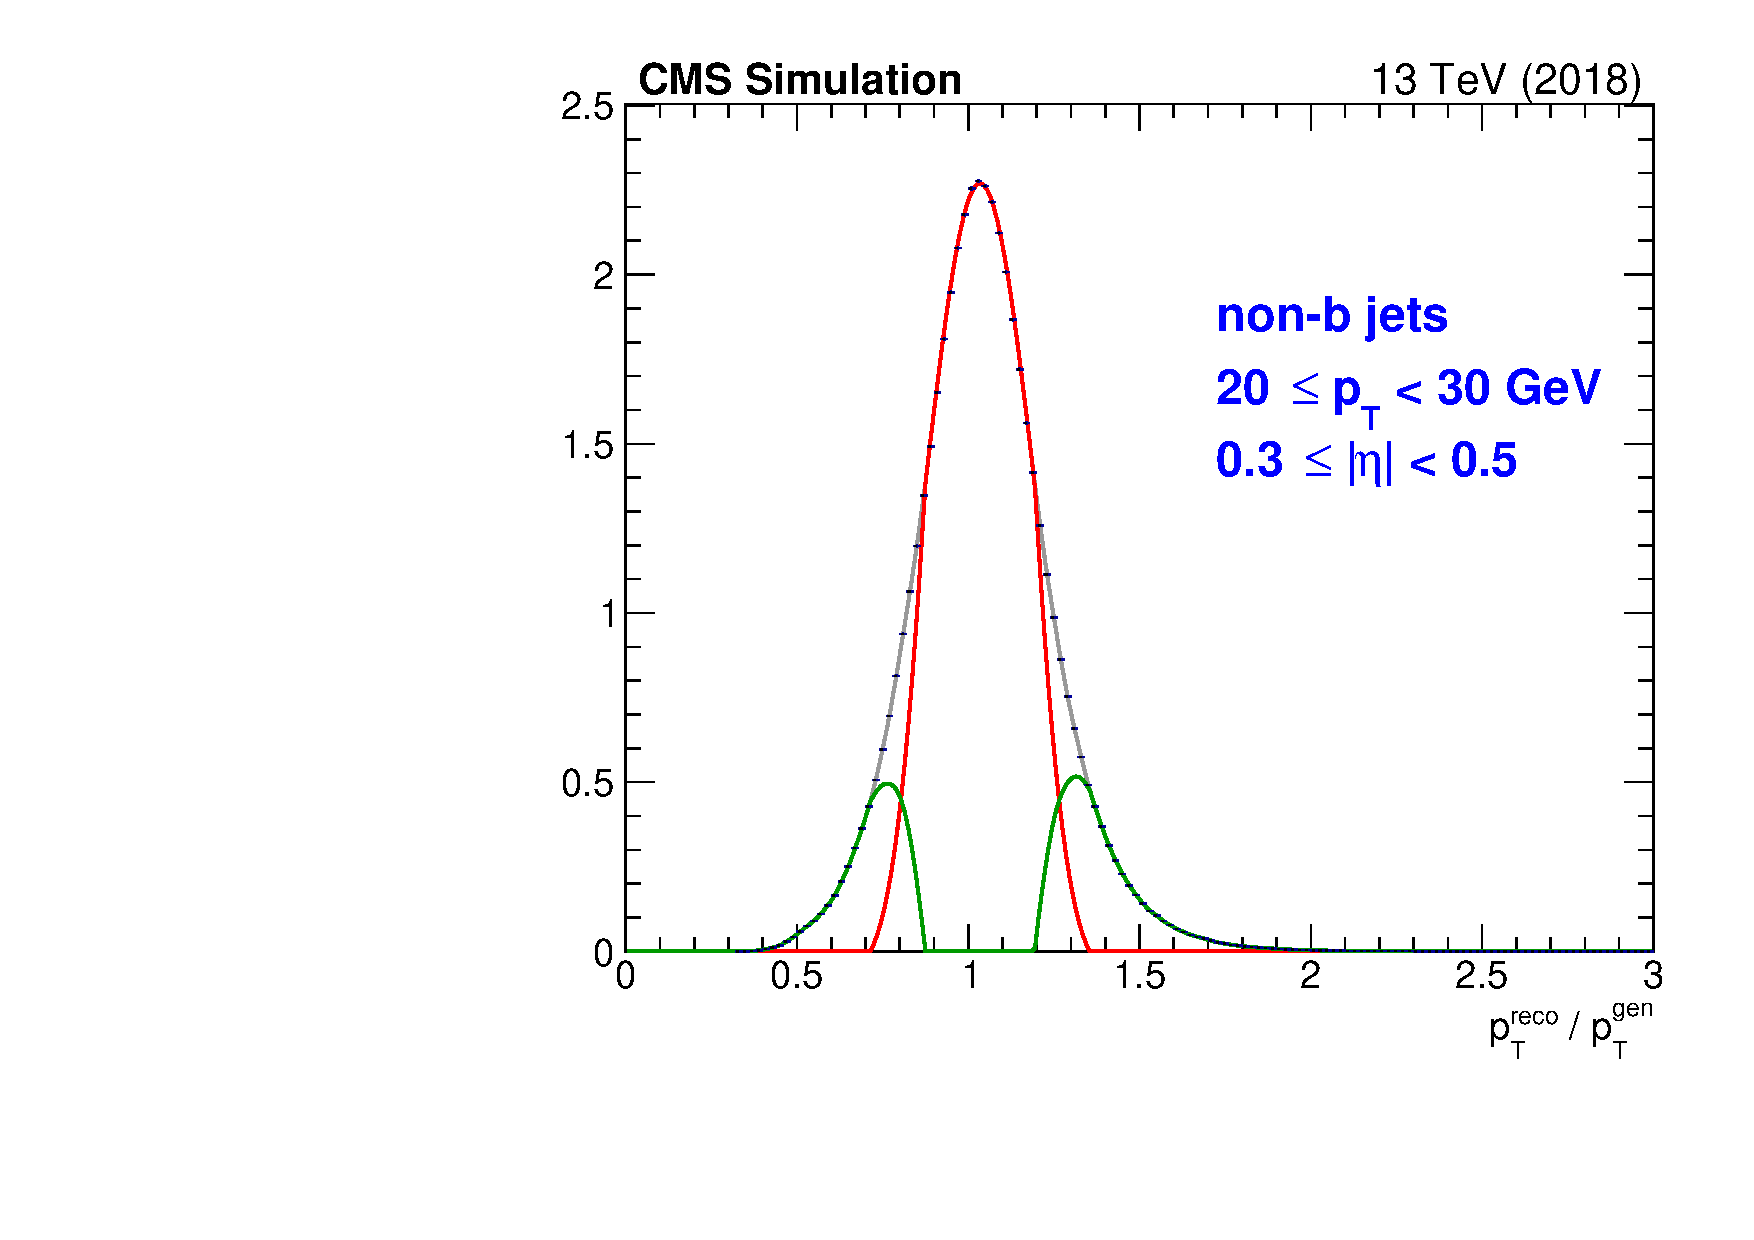
\includegraphics[width=0.45\textwidth]{figs/jetmet/pt01_eta01_nonbjets_lin.pdf}
    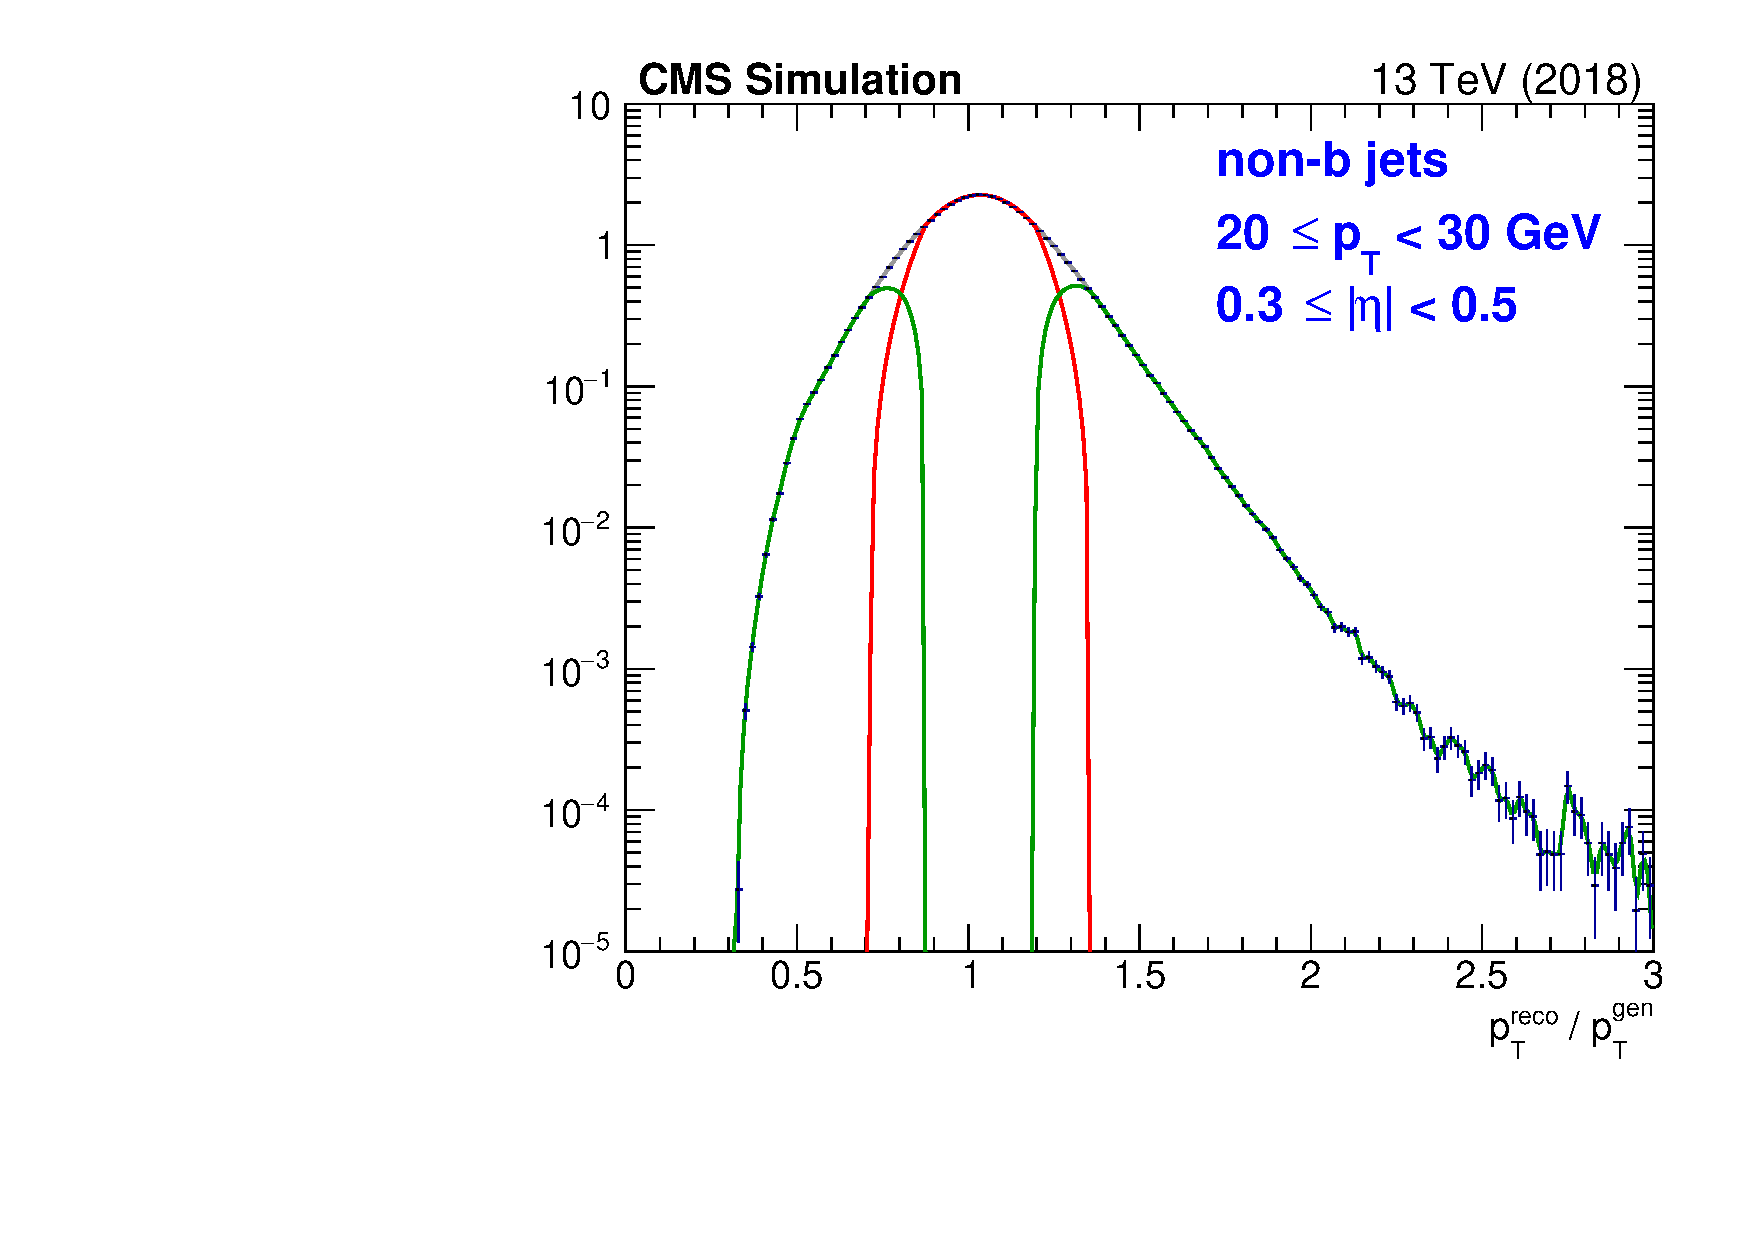
\includegraphics[width=0.45\textwidth]{figs/jetmet/pt01_eta01_nonbjets_log.pdf} \\
    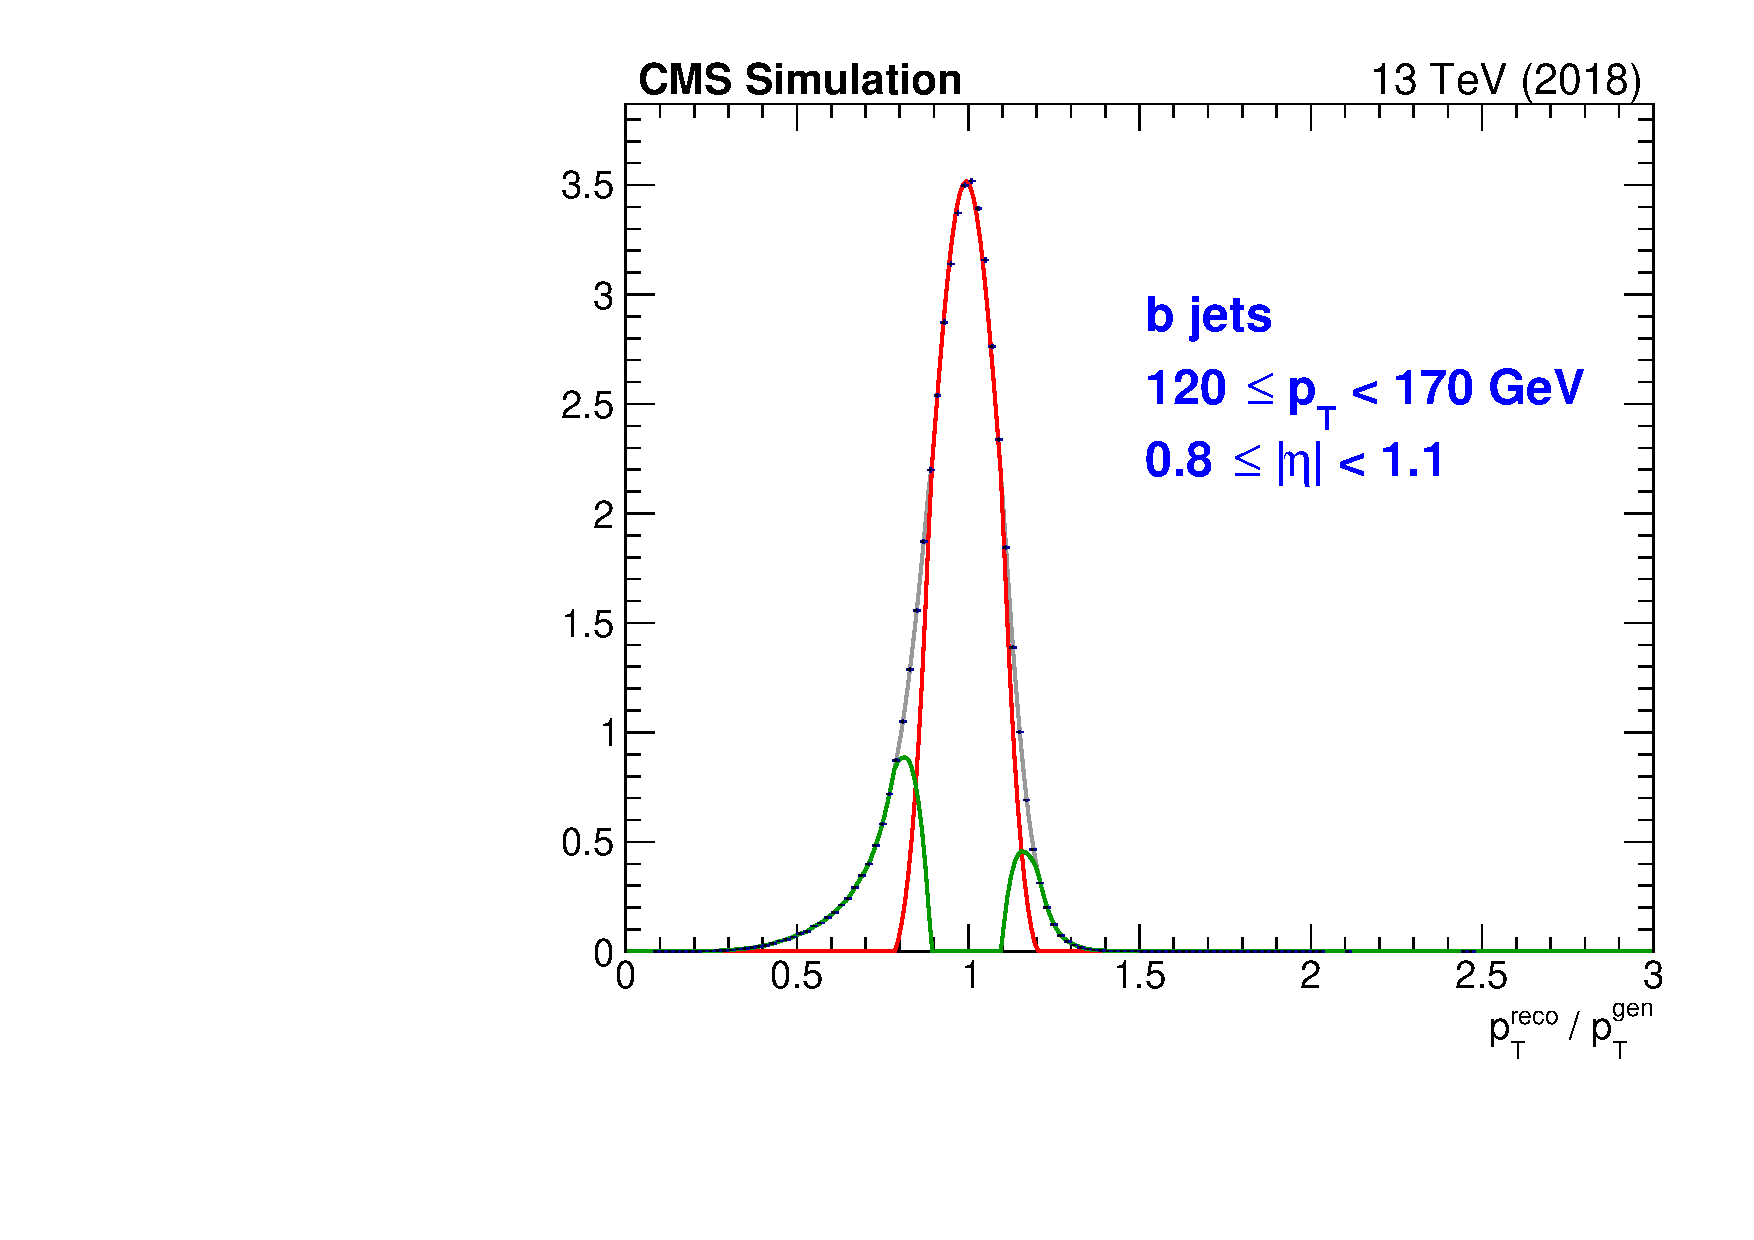
\includegraphics[width=0.45\textwidth]{figs/jetmet/pt05_eta03_bjets_lin.pdf}
    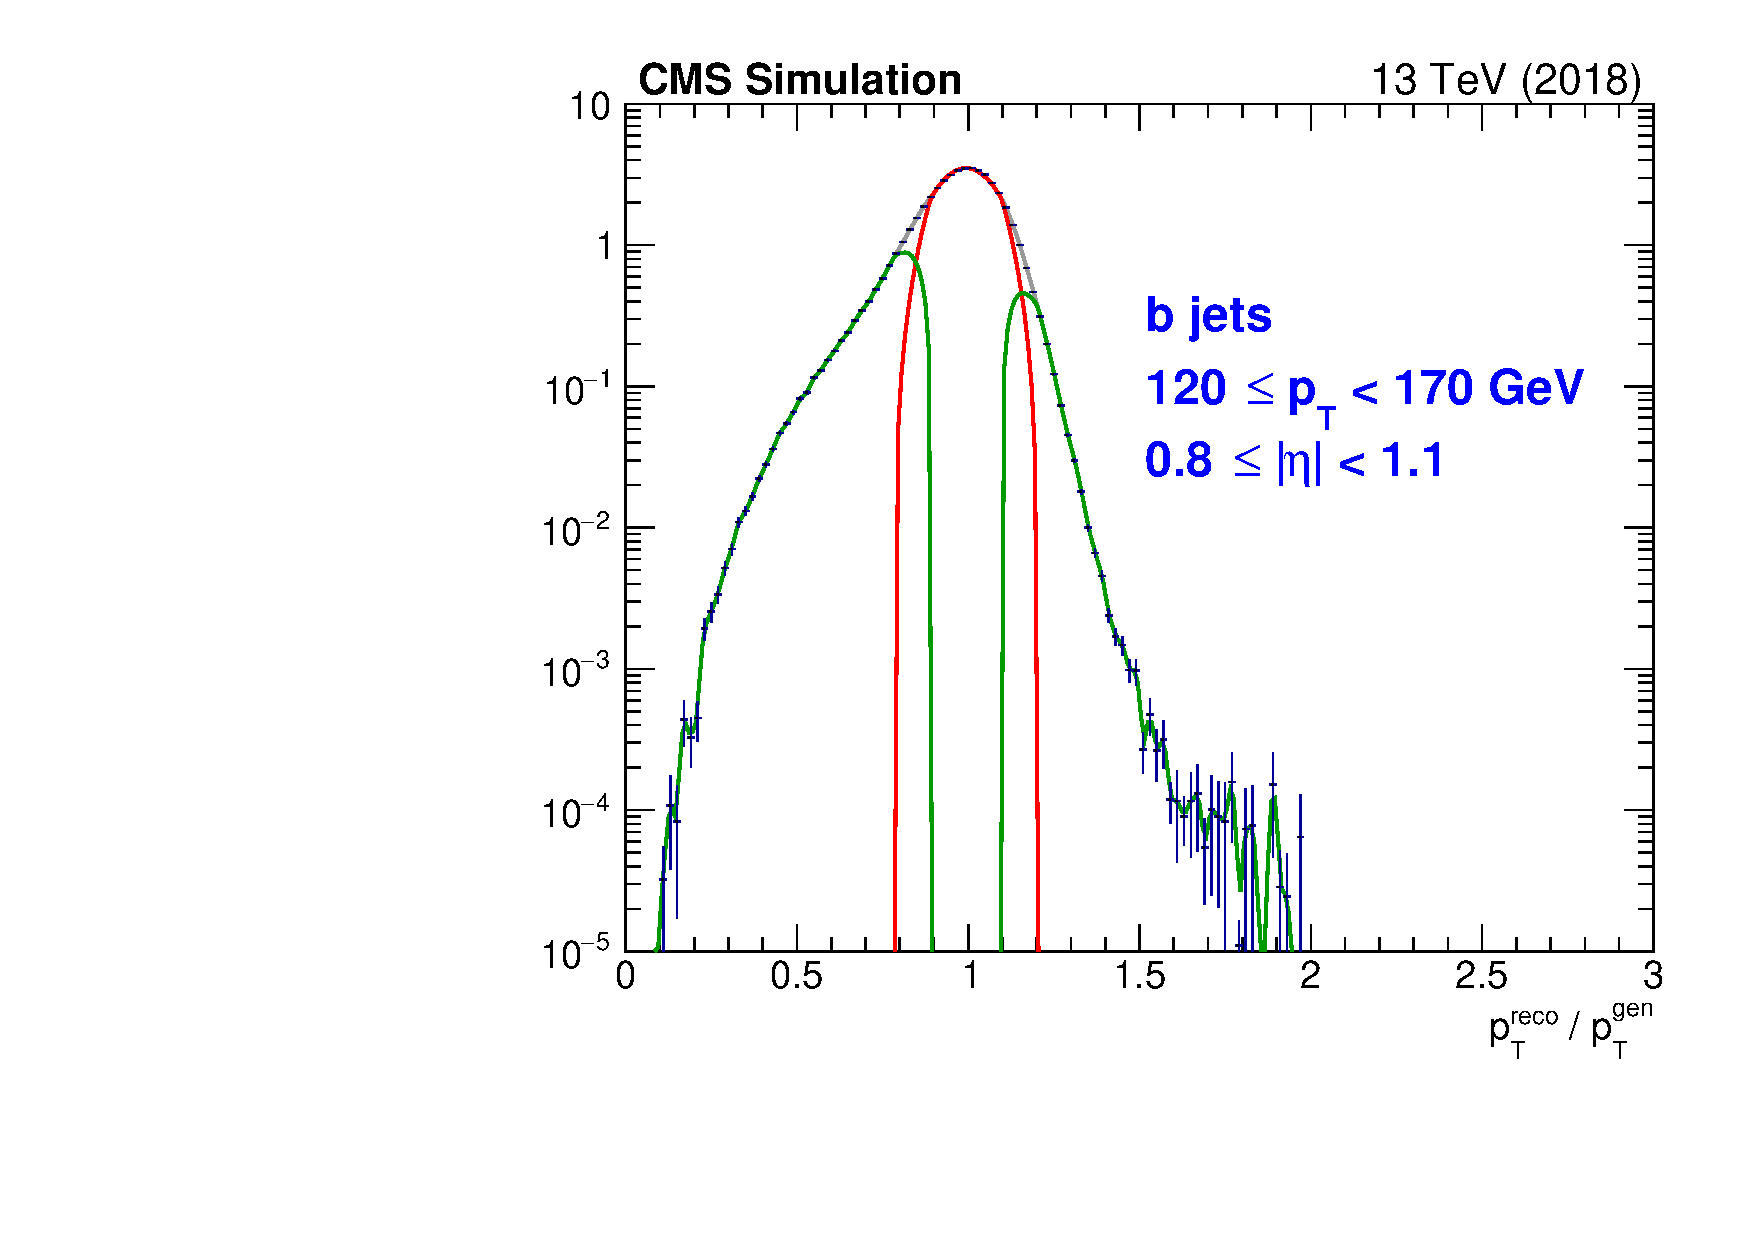
\includegraphics[width=0.45\textwidth]{figs/jetmet/pt05_eta03_bjets_log.pdf} \\
    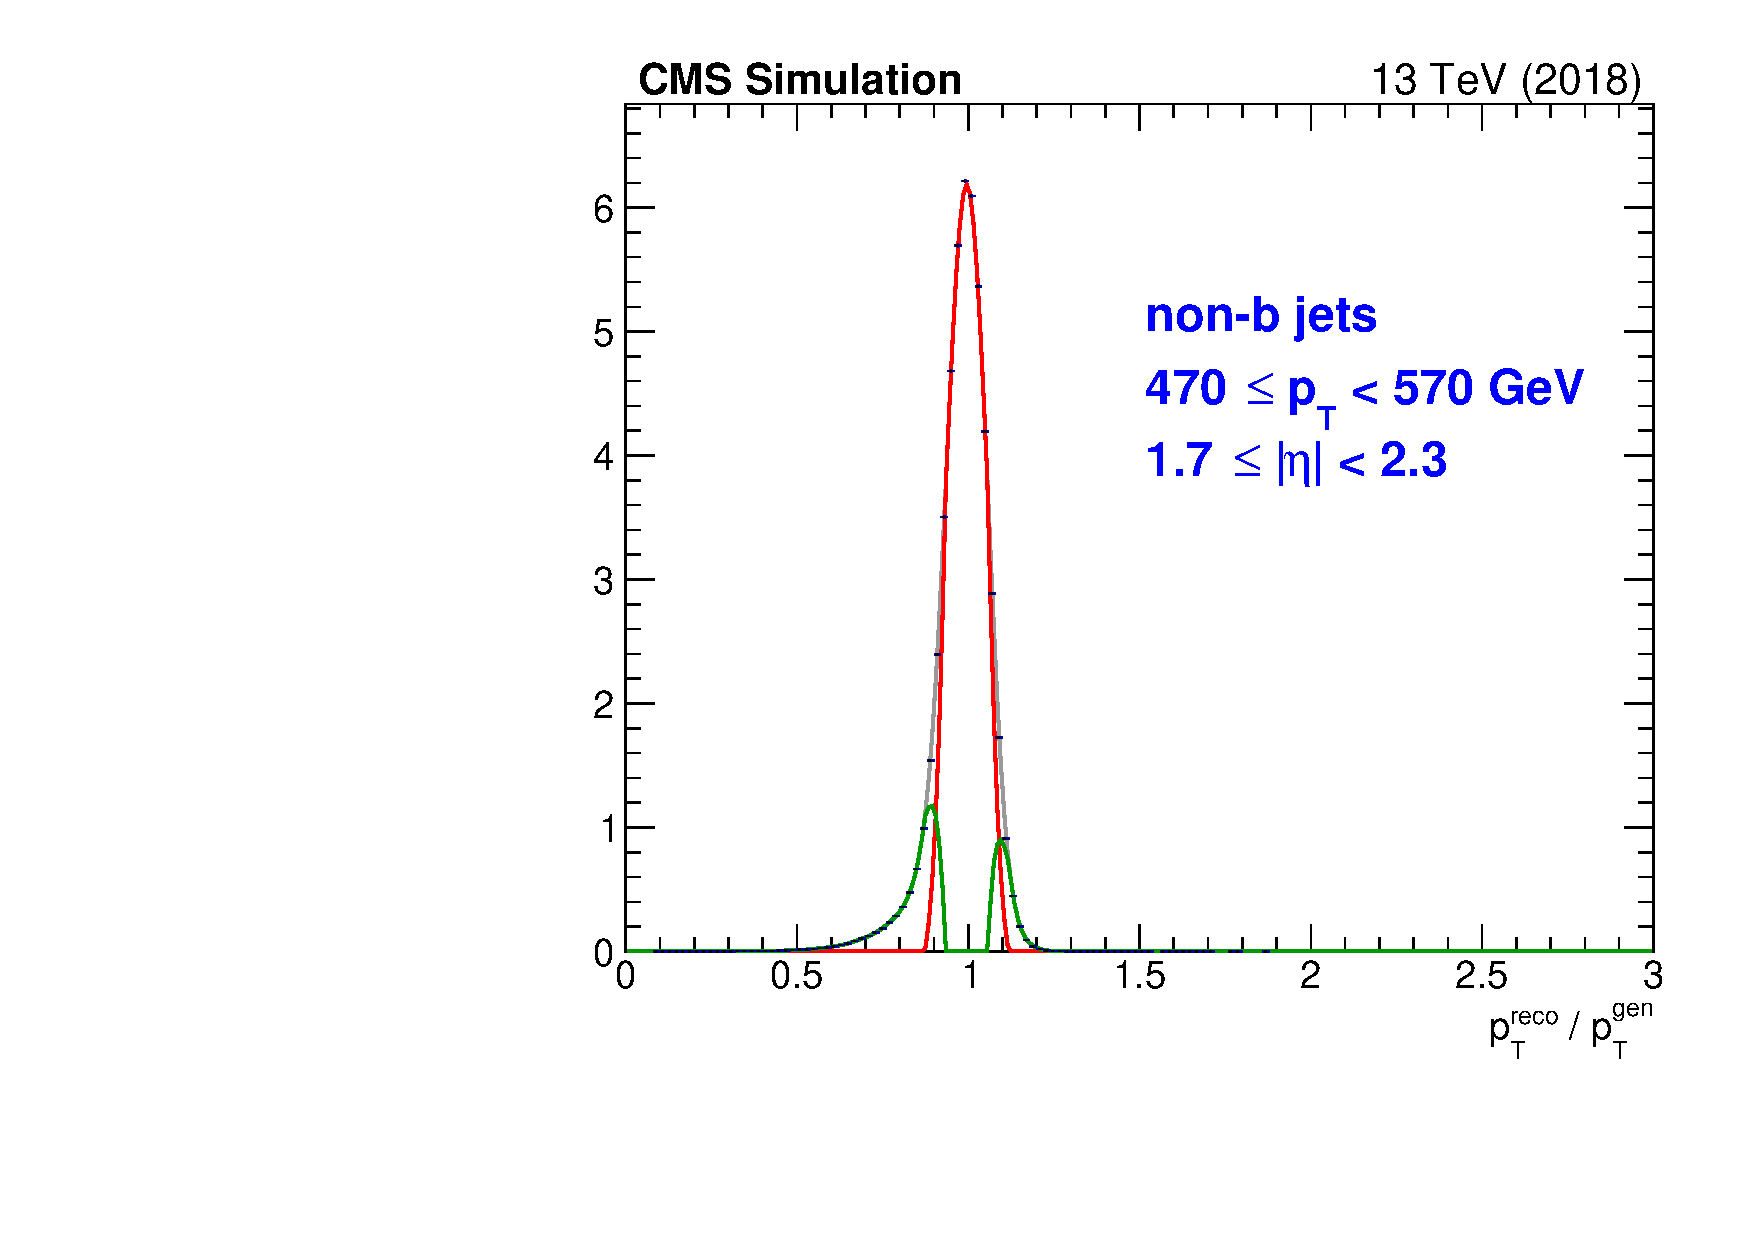
\includegraphics[width=0.45\textwidth]{figs/jetmet/pt10_eta06_nonbjets_lin.pdf}
    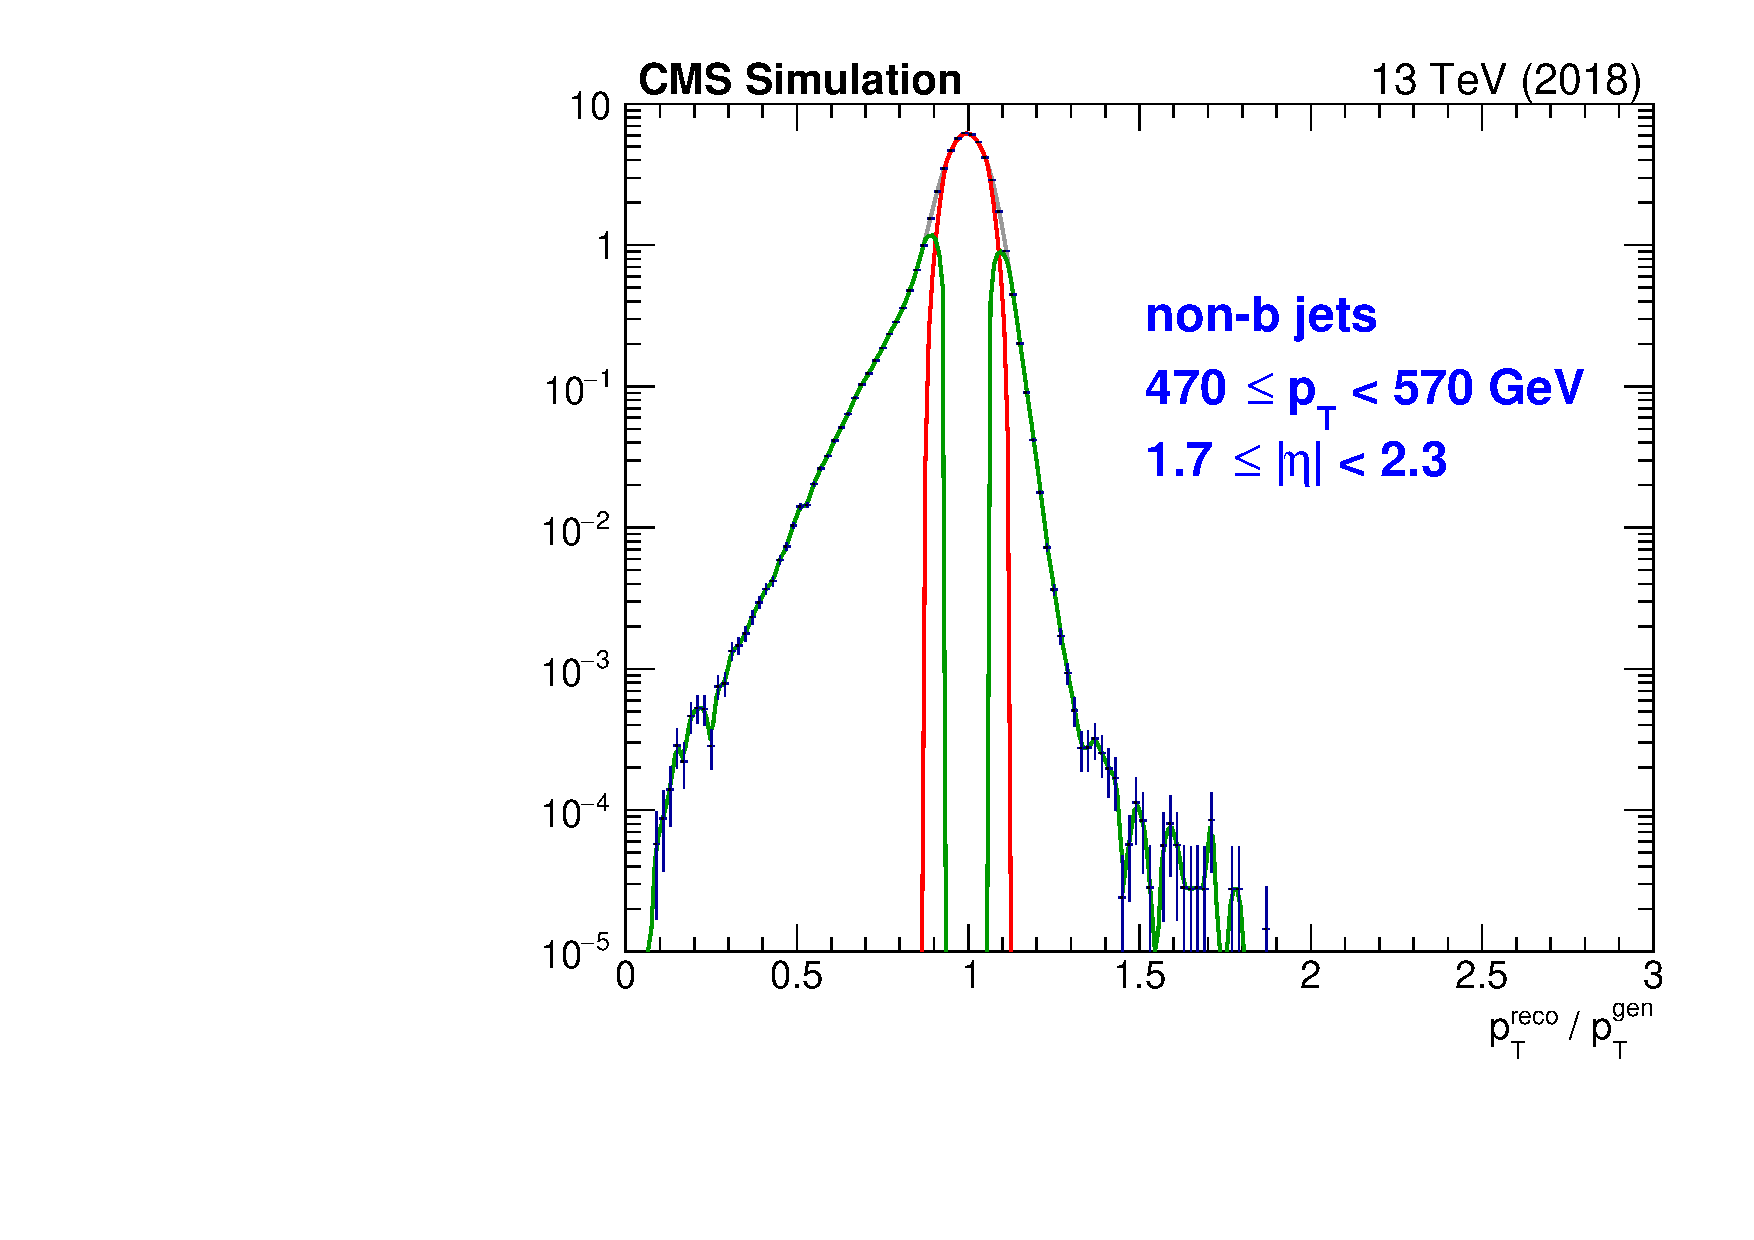
\includegraphics[width=0.45\textwidth]{figs/jetmet/pt10_eta06_nonbjets_log.pdf} \\
    \caption{A selection of three example jet response templates for various \pt/$\eta$/b-jet bins, shown in linear (left) and log (right) scales.
    The dark blue points are the raw templates. The red curves are the fitted gaussian ``cores'' of the templates, and the green
    curves are the ``tails'', as described in Section~\ref{sec:jrt_fits}.
           }
    \label{fig:jrt_examples}
  \end{center}
\end{figure}

\begin{figure}[htbp]
  \begin{center}
    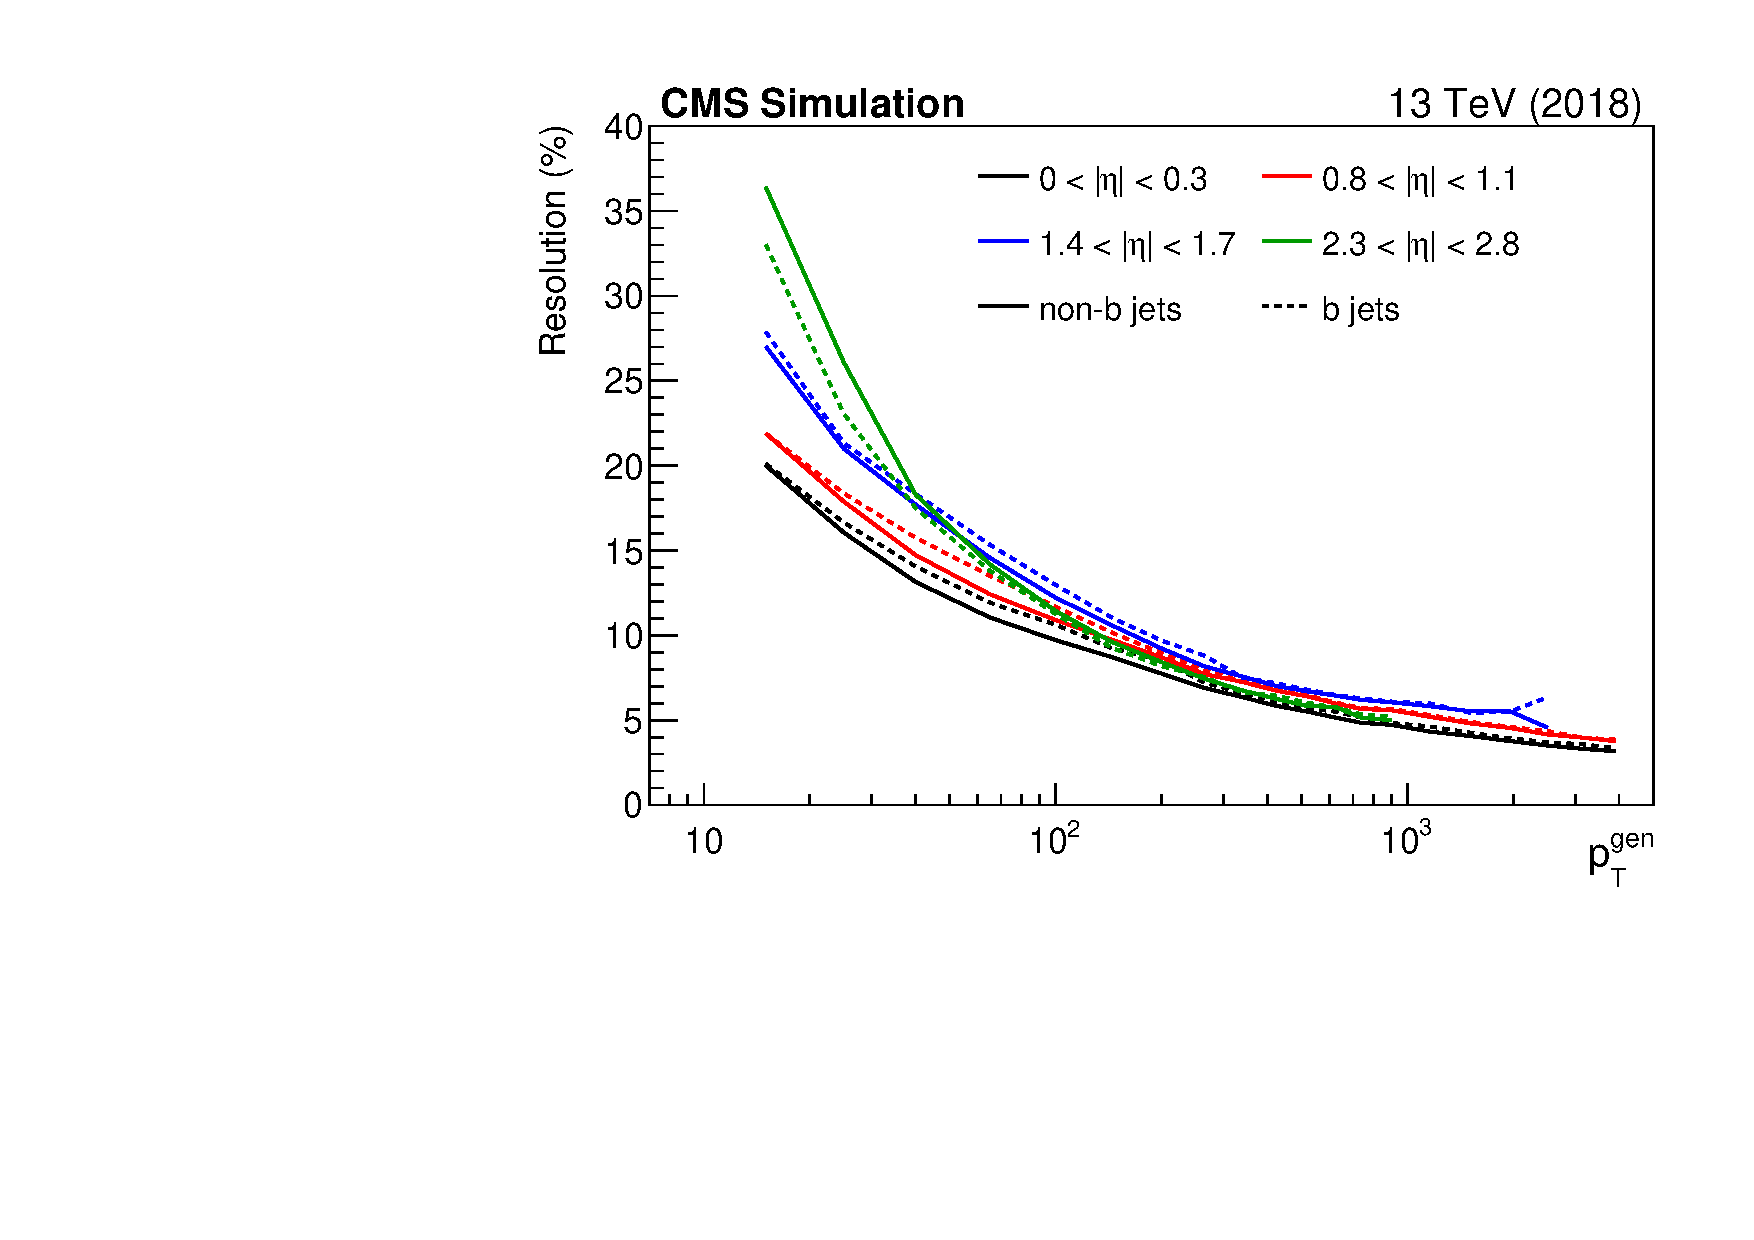
\includegraphics[width=0.49\textwidth]{figs/jetmet/resolution_vs_pt.pdf}
    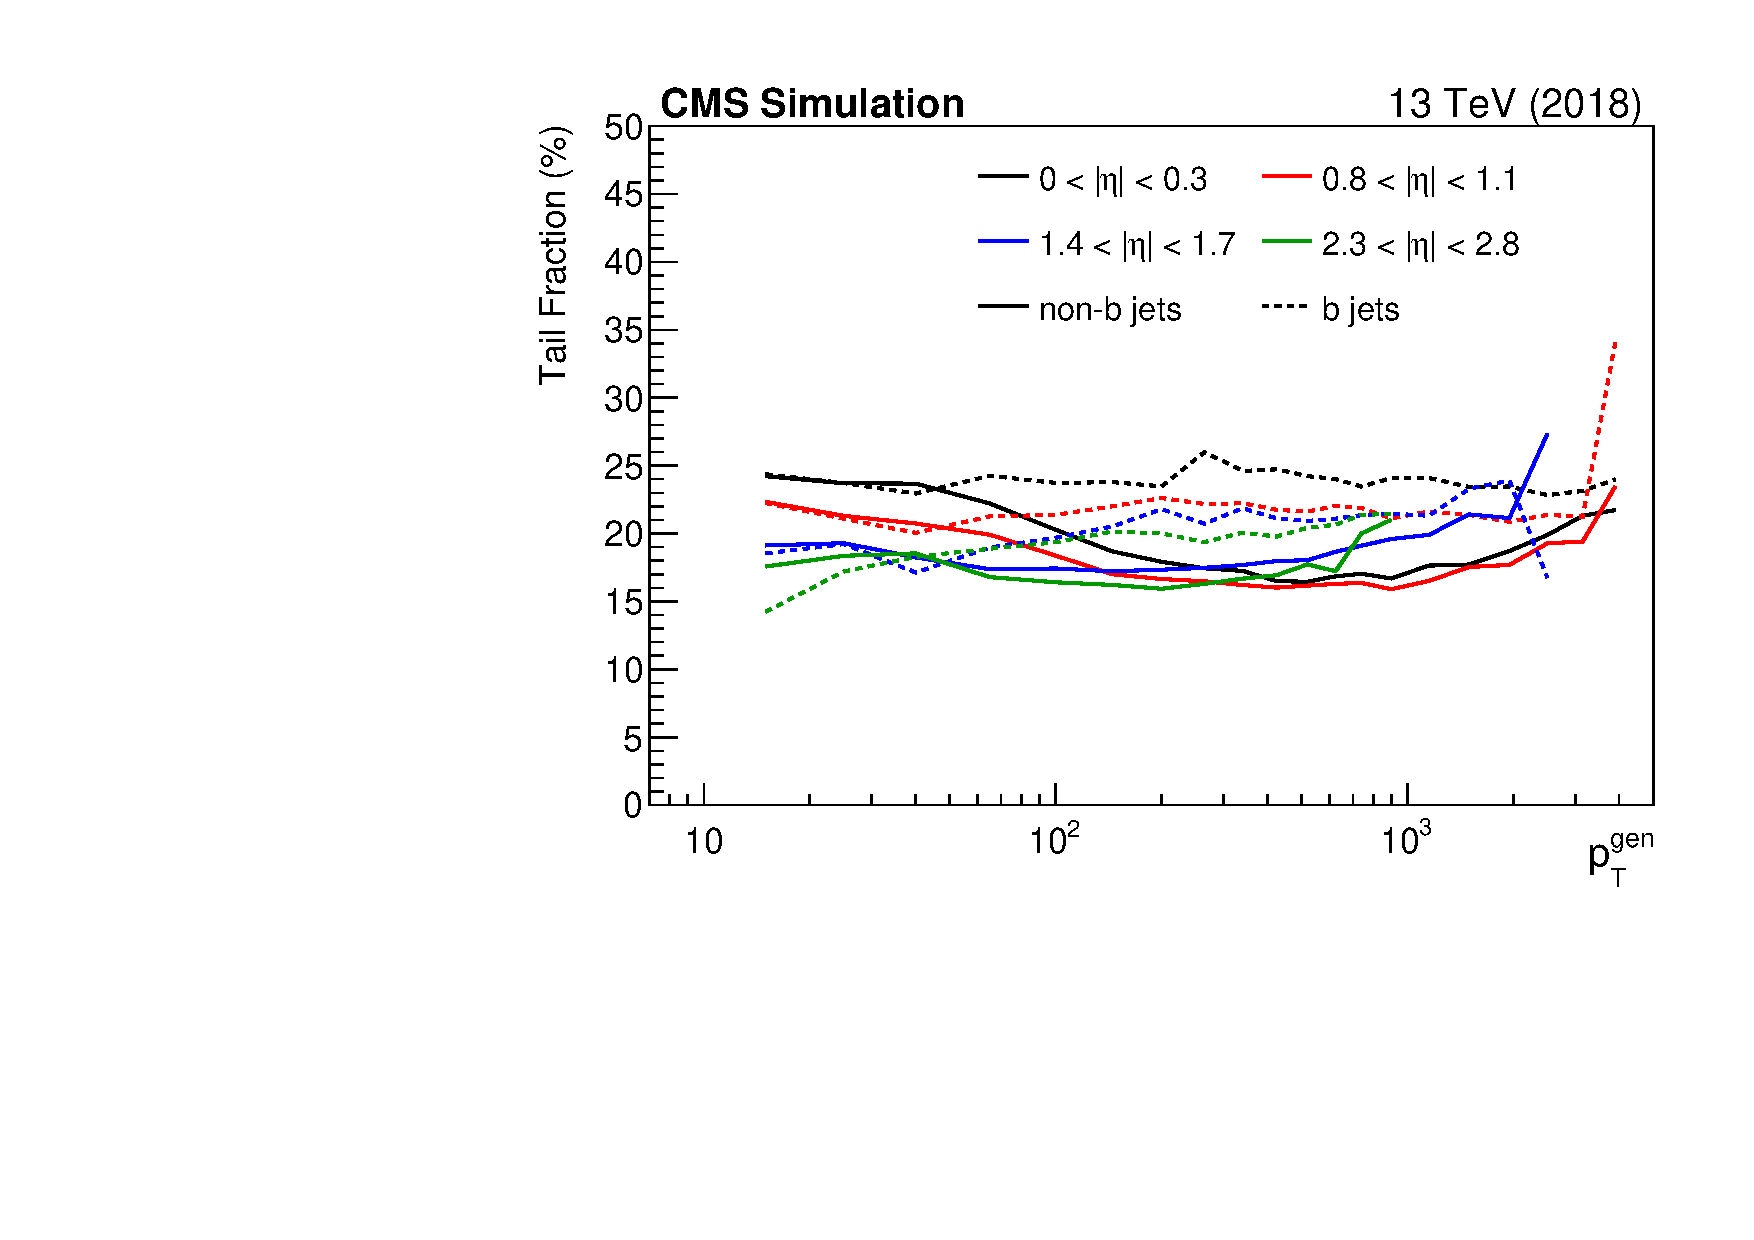
\includegraphics[width=0.49\textwidth]{figs/jetmet/tailfrac_vs_pt.pdf}
    \caption{(left) Jet energy resolution (defined as the width of the fitted gaussian core) as a function of generator-level jet \pt, as measured in Autumn18 MC. 
    Resolution improves as jet \pt increases, and generally degrades as $\eta$ increases.
    (right) The fraction of the jet response function that resides in the fitted tails (as opposed to the gaussian core) as a function of generator-level jet \pt, 
    as measured in Autumn 18 MC. The main feature to notice is that at intermediate \pt,  b jets have a higher probability to be in the tail. This is due to the presence
    of neutrinos from heavy-flavor decay in the jet, which cause the jet energy to be undermeasured and hence enhance the left tail of the templates. At low \pt, the
    tails are driven by other effects so differences between b and non-b jets are not visible.
    }
    \label{fig:jrt_res_pt}
  \end{center}
\end{figure}


\subsection{Gen/reco jet matching}
\label{sec:jrt_matching}

The process for matching gen and reco jets in order to derive jet response templates begins with QCD Monte Carlo,
in which both the generator-level and reconstructed particles have been clustered into jets.
It is important to use gen jets that include neutrinos, as we are interested in modeling jet mismeasurement due
to energy carried away by neutrinos such. Reco jet energies are fully corrected with the same jet energy corrections
as used in the main analysis. Gen jet flavor is determined by identifying the flavor of 
hadrons within the jet cone. Once this is all done, all reco and gen jets with $\pt>10$ GeV are selected and saved.

After selecting the jets, gen and reco jets are matched and JRTs are constructed by 
filling histograms with $\pt^\text{reco}/\pt^\text{gen}$.
The algorithm for matching is outlined here; the reasoning for and effect of various steps are described following.
\begin{enumerate}
\item Skip events that fail any of the MET filters used in the main analysis
\item Find all ``tight pairs'' of reco/gen jets that have $\Delta R$(reco, gen) $<0.3$
\item Find all ``loose pairs'' of reco/gen jets that have $\Delta R$(reco, gen) $<0.5$
\item Identify the reco jets and gen jets that are in more than one loose pair
\item Throw away any tight pairs that contain a jet identified in the previous step
\item Throw away pairs where in which the reco jet is within one of the manually-identified calorimeter holes
\item Throw away pairs where in which the reco jet fails tight jet ID
\item Throw away pairs where in which the reco jet fails loose pileup jet ID
\item For all remaining tight pairs, identify the correct \pt/$\eta$-binned histograms and fill:
  \begin{itemize}
    \item b jet histogram with weight \\
    \hphantom{1 cm}$w_\text{b}=\varepsilon_\text{b-tag}$(\pt, $\eta$, gen flavor) $\times$ $SF_\text{b-tag}$(\pt, $\eta$, gen flavor),
    \item non-b jet histogram with weight \\
    \hphantom{1 cm}$w_\text{non-b} = 1-w_\text{b}$,
  \end{itemize}
  where $\varepsilon_\text{b-tag}$ is the efficiency for tagging a particular flavor of gen jet, as measured in MC, and $SF_\text{b-tag}$ is 
  the CMS-derived scale factor to correct this efficiency for known differences between data and MC.
\end{enumerate}

Step 1 rejects entire events that fail one of the MET filters applied in the main analysis.
These guard against certain kinds of mis-reconstruction that can enhance the tails of the
jet response functions. Most notably, the EcalDeadCellTriggerPrimitive and HBHENoise filters
reject events where there is energy in calorimeter regions known to be down/noisy (leading to 
fake energy, and enhancement of the right tails), and the BadChargedCandidate and BadPFMuon
filters reject events containing badly reconstructed high-\pt tracks (which also enhance
the right tails). Since we reject these events in the main analysis, we also reject
jets from such events here to avoid false tails in the templates 
(see Fig.~\ref{fig:jrt_matching_effect} (right) for an example of the effect on a template)

Steps 2 through 5 identify pairs of gen and reco jets with $\Delta R<0.3$, but with the crucial caviat that 
\emph{there are no additional matches within} $\Delta R<0.5$. This protects against one of the largest fake sources
of tails in the measured templates: the ``splitting'' of gen and/or reco jets. This can happen in three distinct ways:
\begin{itemize}
  \item A single gen jet is reconstructed as multiple reco jets, and gets matched to one. 
  This enhances the left tail of the templates, as the matched reco jet only has a fraction of the energy.
  \item Multiple gen jets are reconstructed as a single reco jet. This enhances the right tail of the 
  templates, as the matched gen jet only has a fraction of the energy.
  \item There are multiple nearby gen and reco jets, but energy/particles are distributed differently 
  among the gen jets compared to reco. This enhances both tails, depending on how the energy distribution
  and matching happens.
\end{itemize}
Requiring that there are no secondary nearby gen (reco) jets within $\Delta R<0.5$ of the reco (gen) jet protects against these scenarios.
The effect on a sample template is shown in Fig.~\ref{fig:jrt_matching_effect}. 
The reduction in the tails after applying this cut is seen to be quite large.

\begin{figure}[htbp]
  \begin{center}
    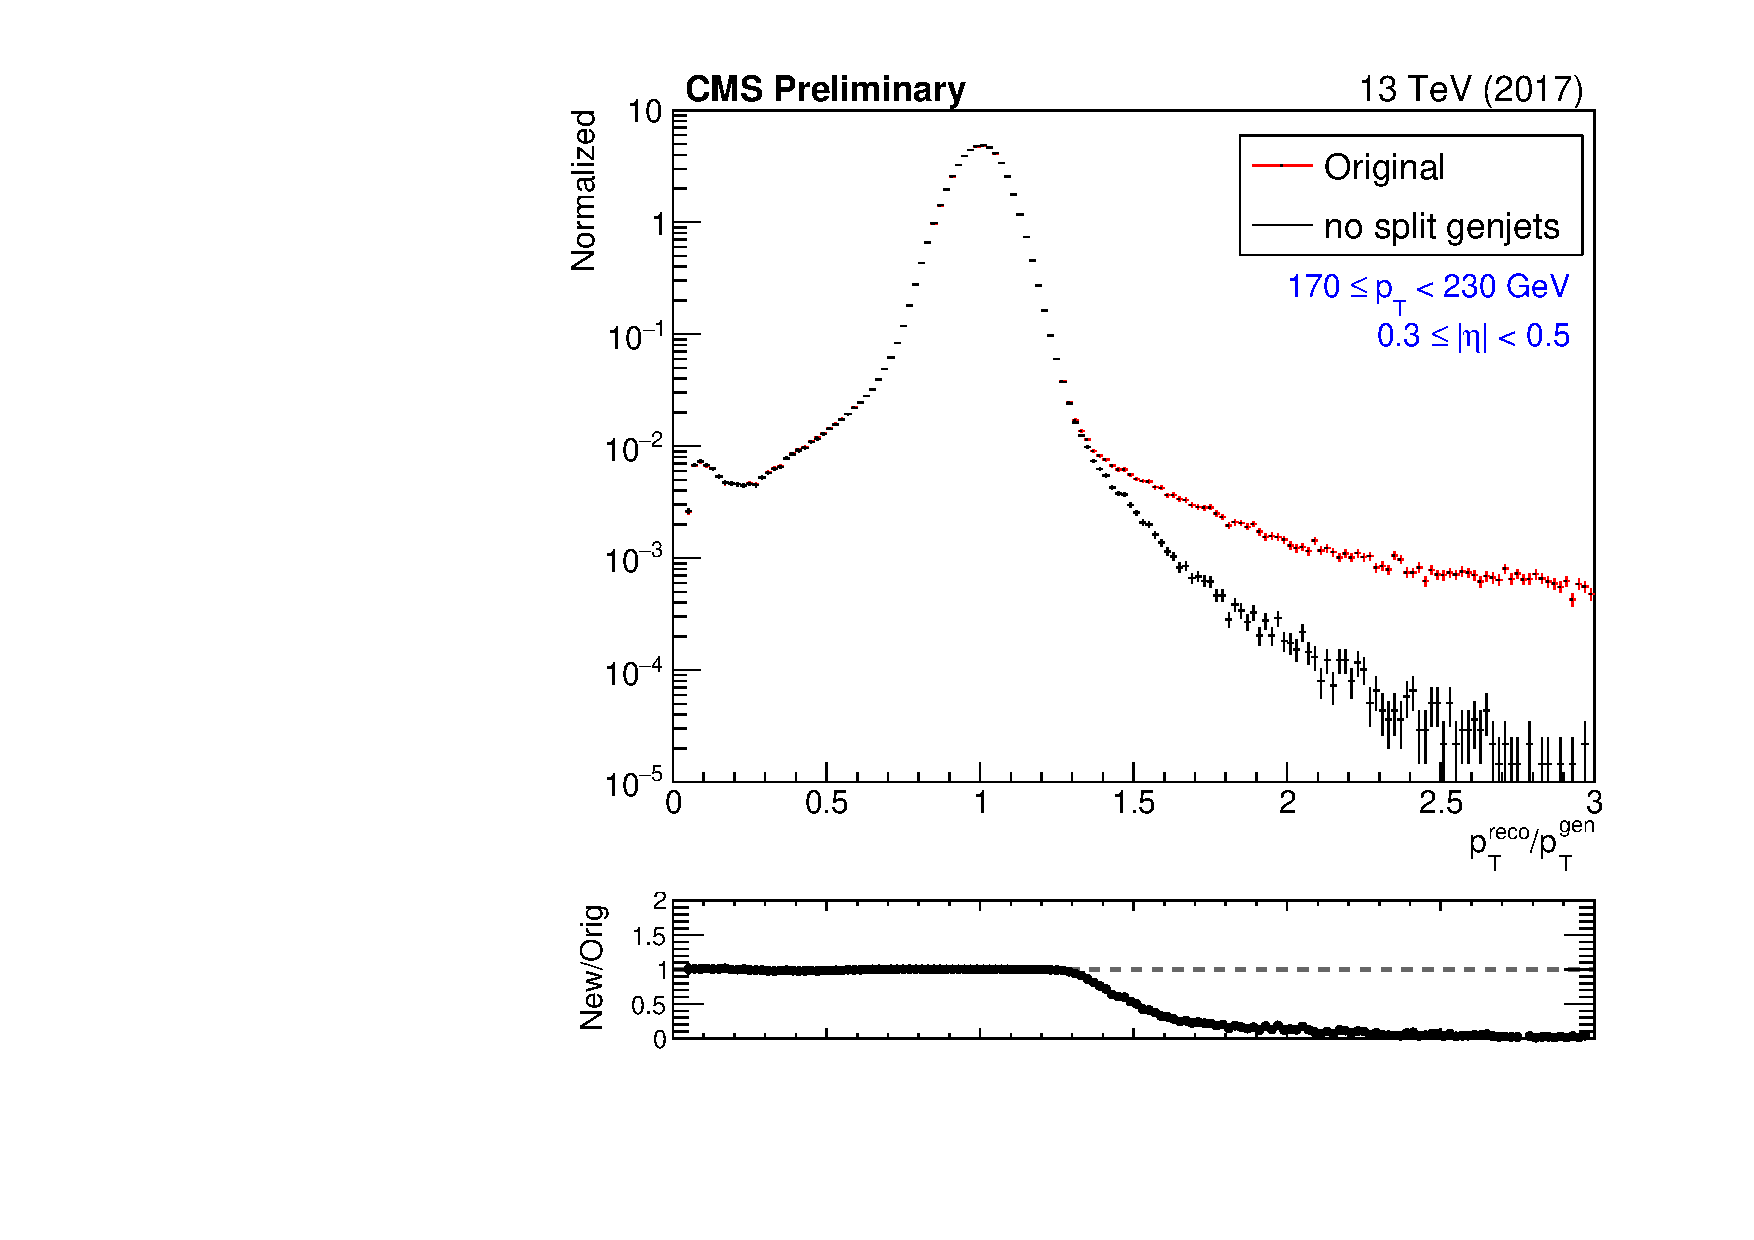
\includegraphics[width=0.325\textwidth]{figs/jetmet/compare_noSplitGen.pdf}
    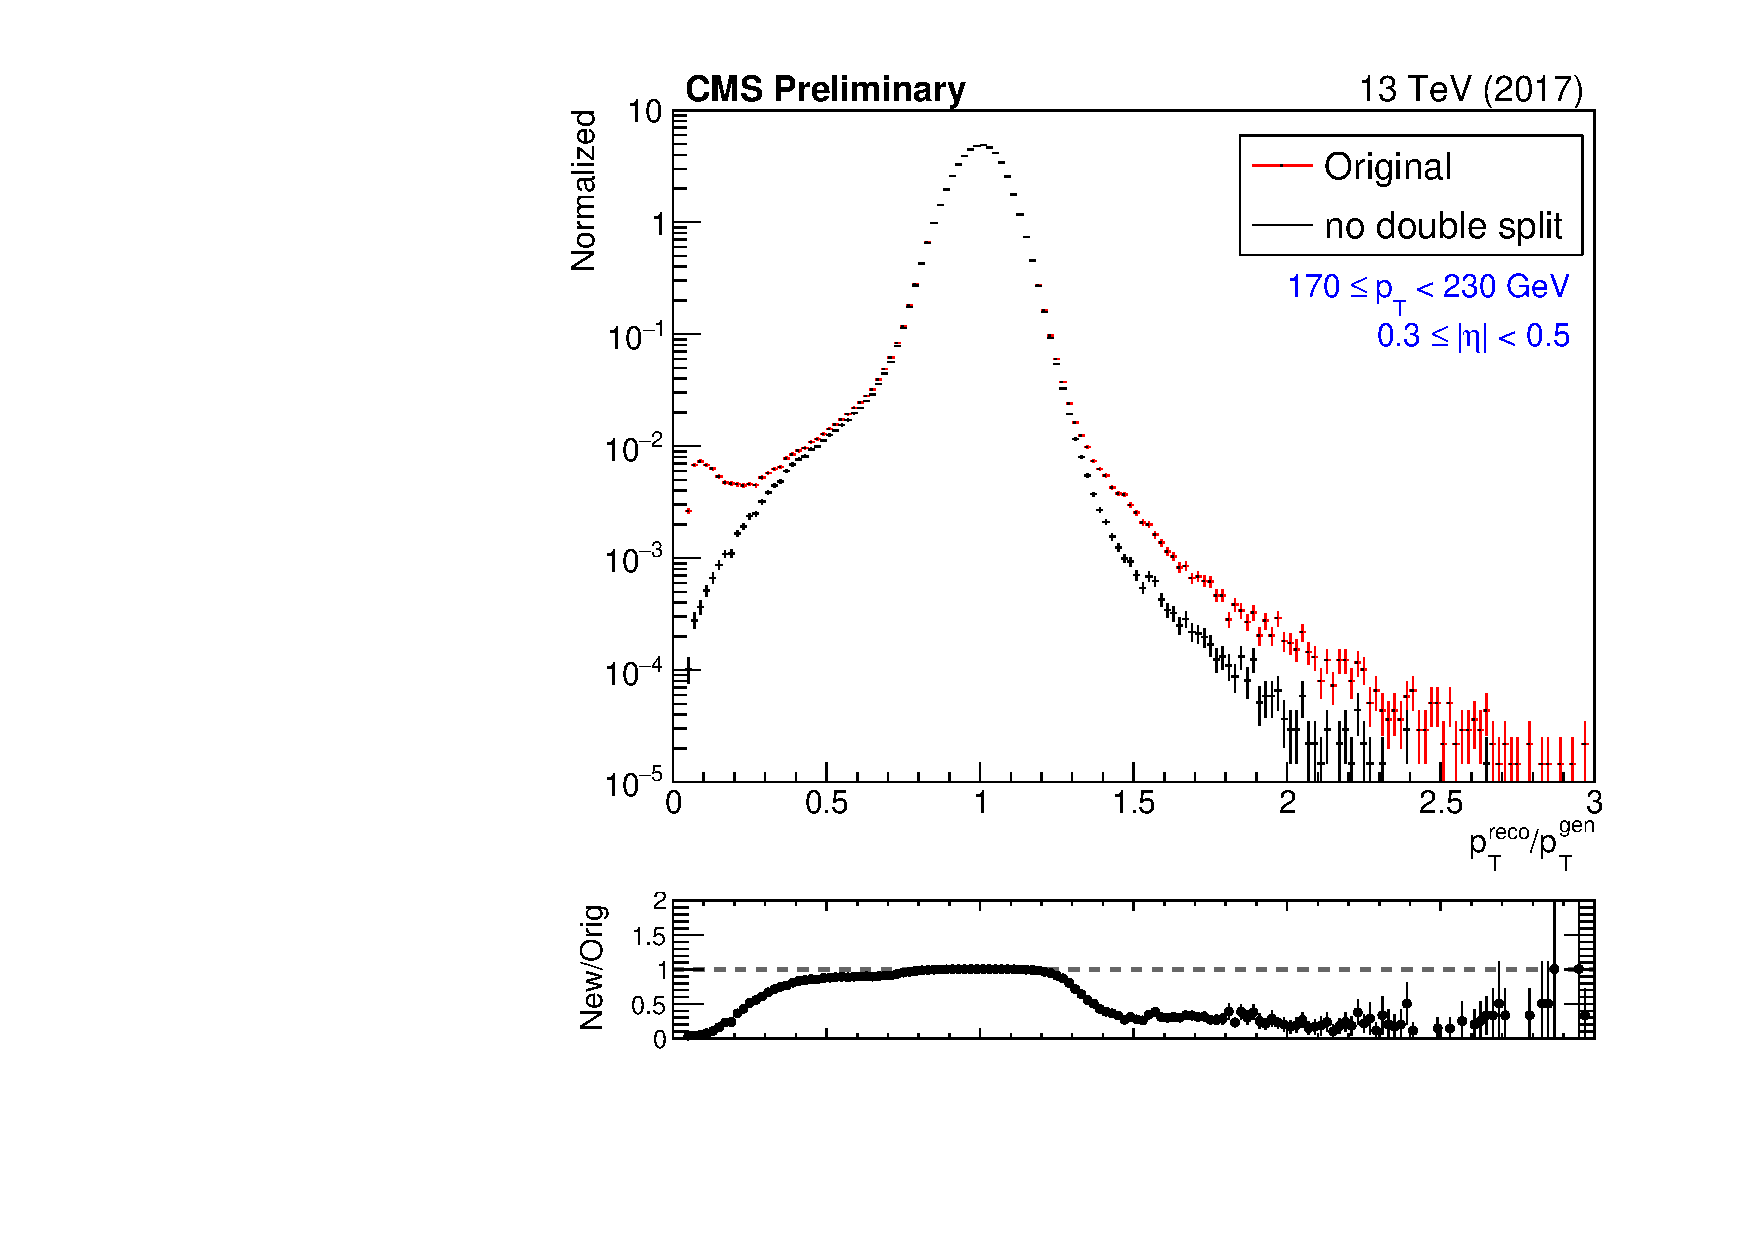
\includegraphics[width=0.325\textwidth]{figs/jetmet/compare_noDoubleSplit.pdf}
    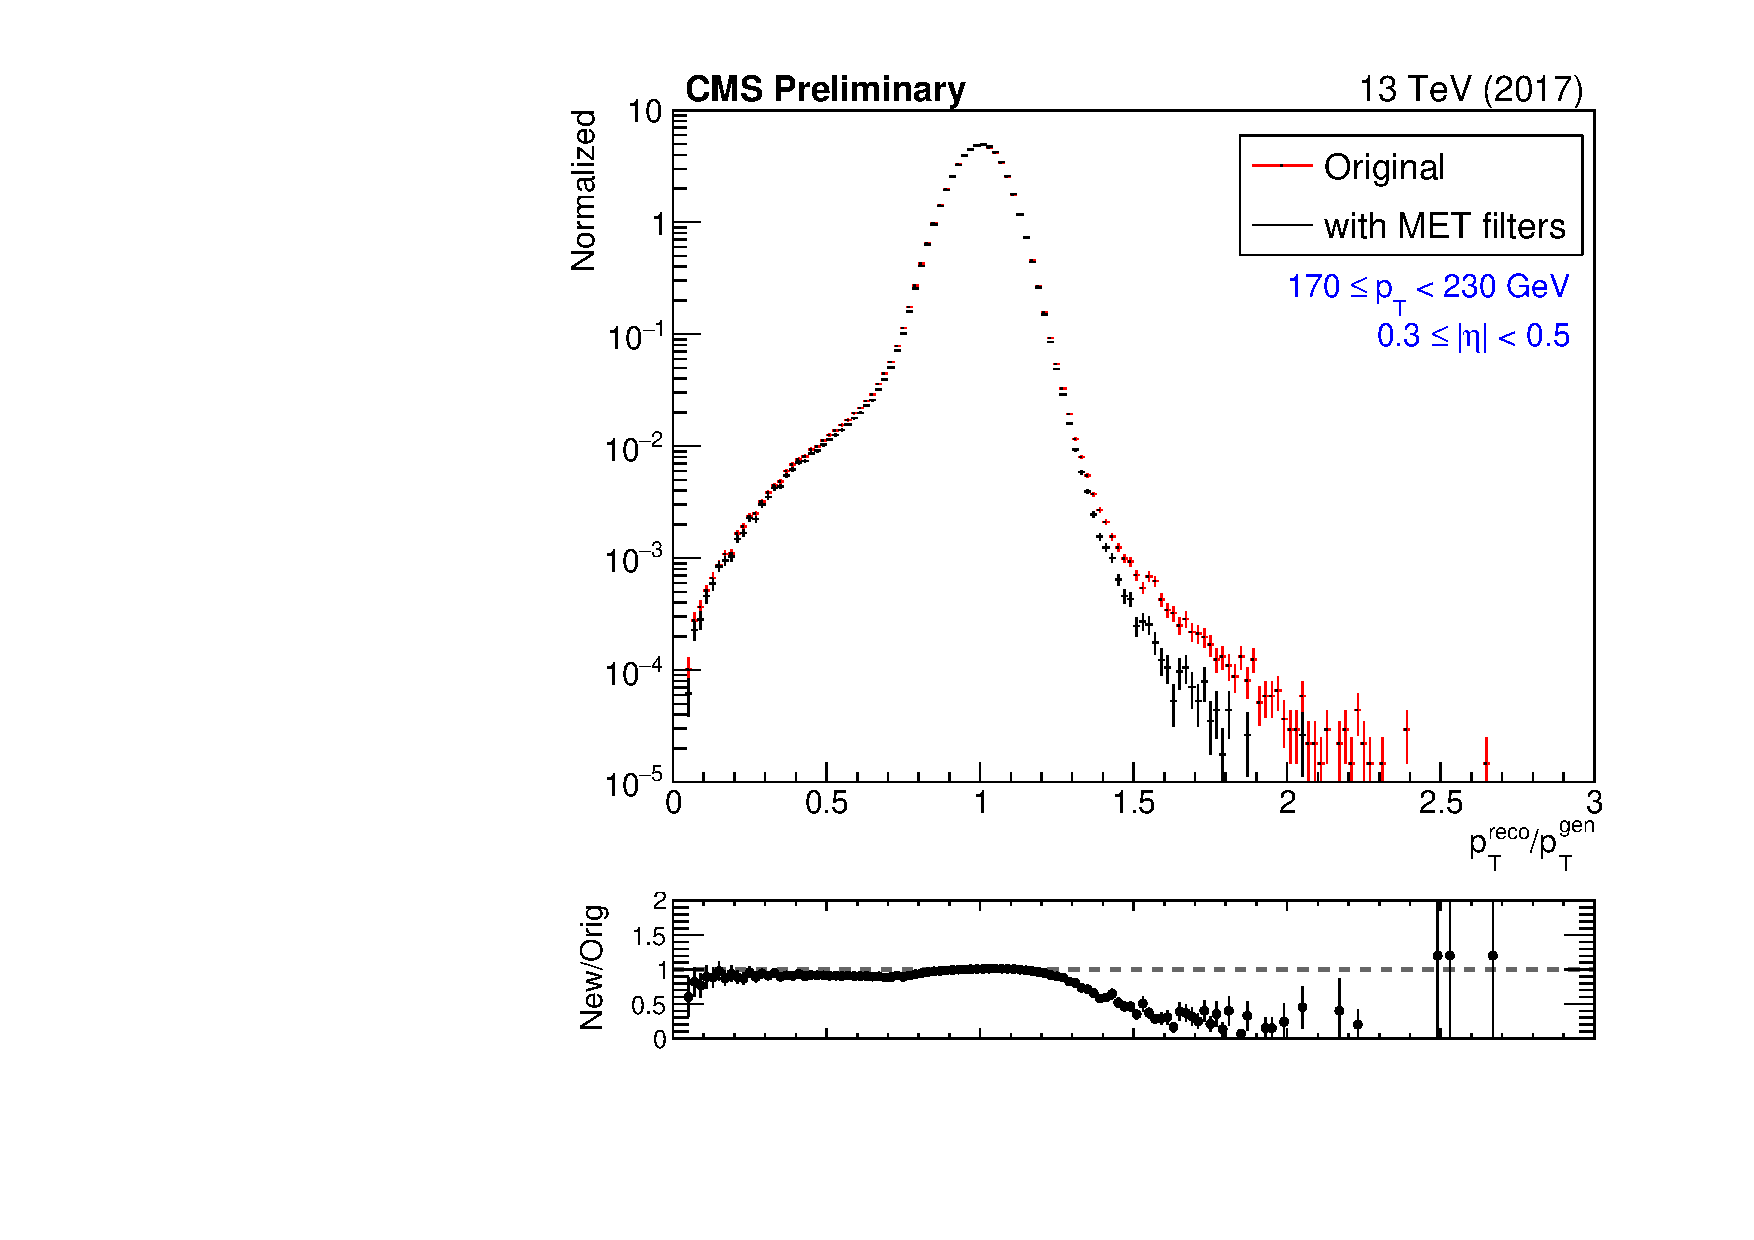
\includegraphics[width=0.325\textwidth]{figs/jetmet/compare_metFilters.pdf}
    \caption{The effect of various cuts applied during the matching on an example template (non-b jet, $170 \leq \pt < 230$ GeV, $0.3 \leq |\eta| < 0.5$).
    (left) Requiring \emph{exactly} 1 gen jet within $\text{dR}<0.3$ of a reco jet, instead of at least one. This removes ``split'' gen jets.
    (center) Requiring that there are no secondary nearby gen (reco) jets within $\text{dR}<0.5$ of the reco (gen) jet. This protects
    against splitting in both directions, so reduces both tails.
    (right) Applying MET filters and rejecting jets from events that fail. This removes bad reconstructions (e.g. fake high-\pt track) and
    primarily reduces the right tail.
    }
    \label{fig:jrt_matching_effect}
  \end{center}
\end{figure}

Step 6 throws away pairs involving a reco jet in one of a number of manually-identified ``dead'' spots in the detector.
When plotting an $\eta-\phi$ map of the jets with small ($<$0.5) $\pt^\text{reco}/\pt^\text{gen}$ values,
we observe a number of ``hot-spots'', corresponding to calorimeter regions that are dead or off in the simulation.
These do not generally correspond to real effects in the data, and lead to artificially large left tails in the templates.
We identify these regions (separately for each year) and remove any jet pairs that contain a reco jet in one of these regions.
Fig.~\ref{fig:jrt_ecalDeadCell} shows these cells highlighted for 2017 simulation on the left, and
the effect on an example template on the right.

\begin{figure}[htbp]
  \begin{center}
    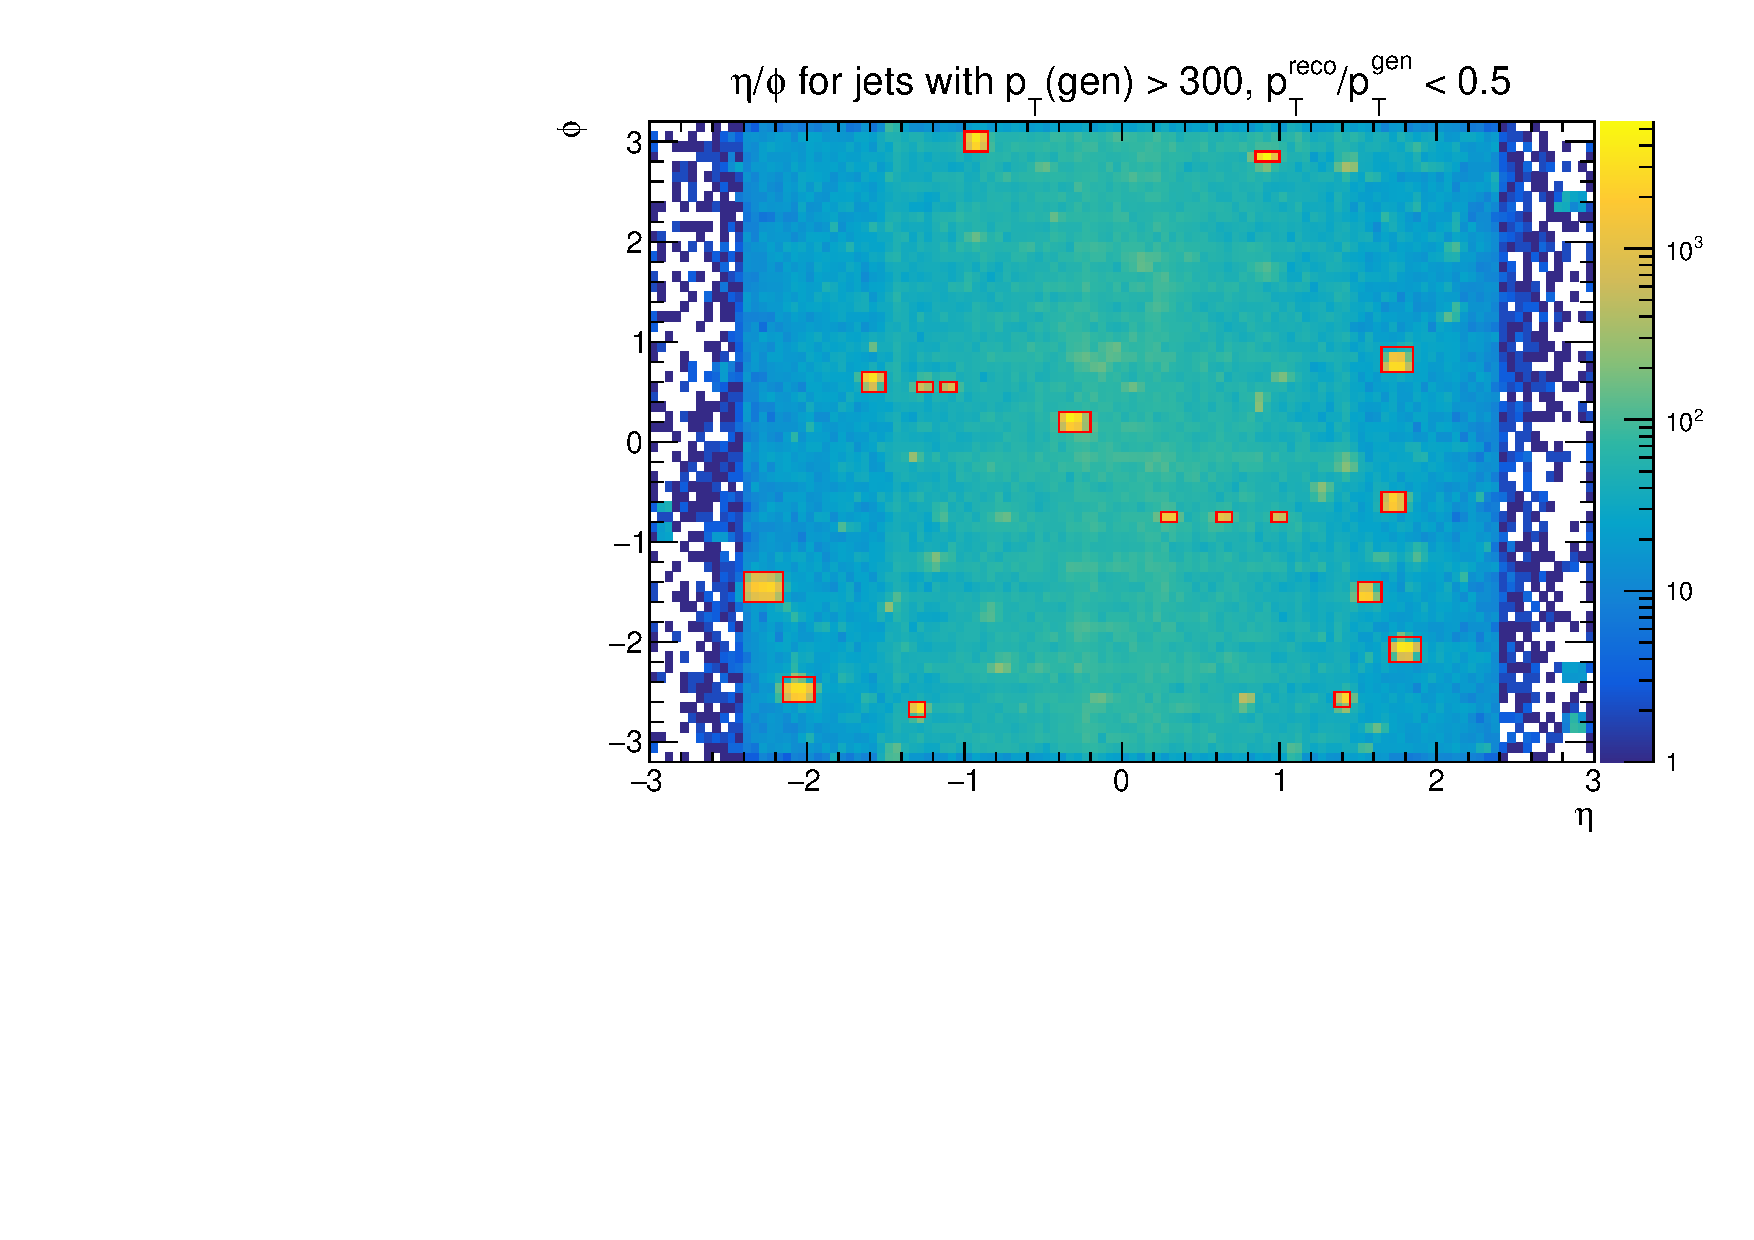
\includegraphics[width=0.54\textwidth]{figs/jetmet/ecalDeadCells.pdf}
    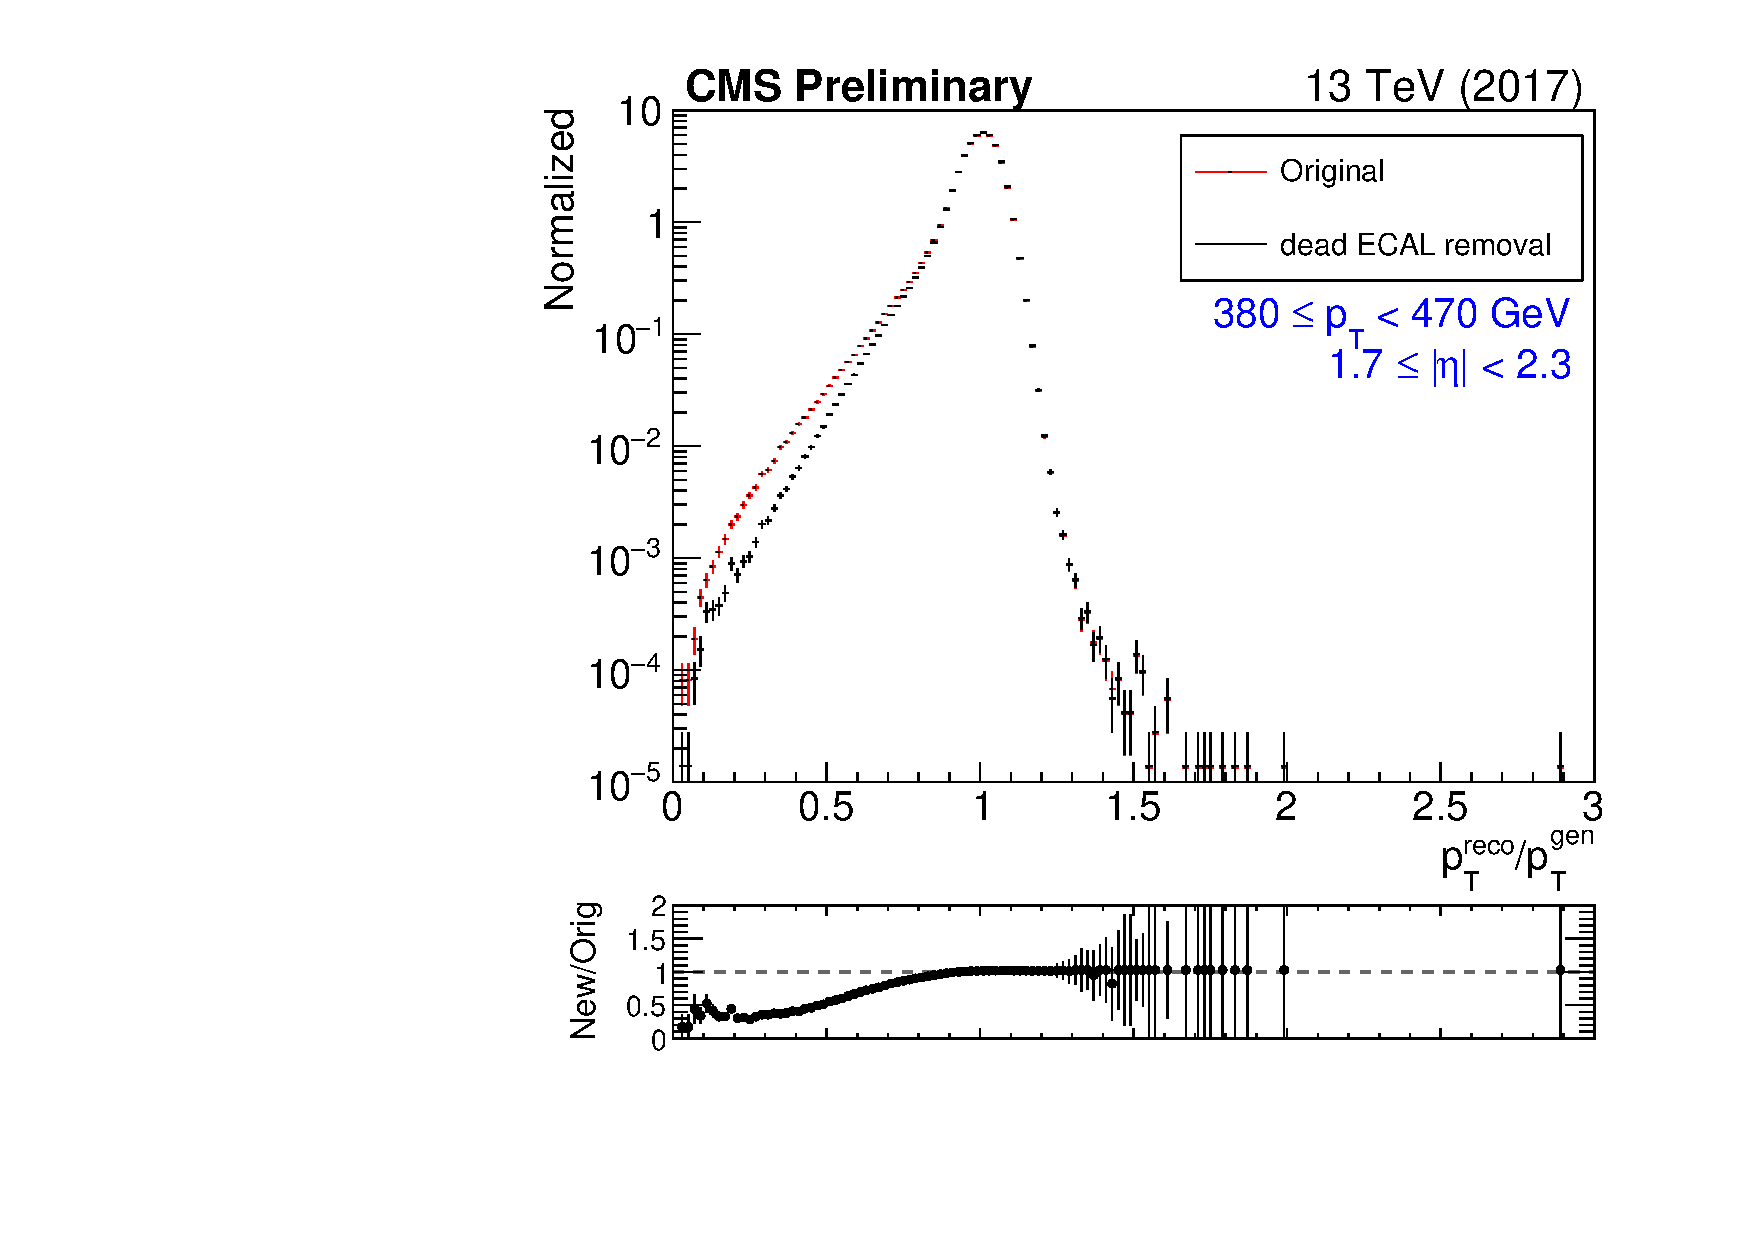
\includegraphics[width=0.45\textwidth]{figs/jetmet/compare_ecalDeadCell.pdf}
    \caption{(left) an $\eta-\phi$ map for jet pairs with $\pt^\text{gen}> 300$ GeV and
    $\pt^\text{reco}/\pt^\text{gen} < 0.5$ from 2017 simulation. Identified hot-spots
    are outlined in red. Pairs with reco jets in these regions are not used.
    (right) The effect of this removal on an example template. Relatively large reductions
    in the left tail are seen for templates containing affected regions.
    }
    \label{fig:jrt_ecalDeadCell}
  \end{center}
\end{figure}

Step 7 rejects pairs in which the reco jet fails tight jet ID.
In the main analysis, we reject the entire event if any jet with $\pt>30$ GeV
fails this ID. We apply the same ID here to avoid including these jets in 
the templates. It is found to have minimal effect, except for very high eta ($|\eta|>4.0$).

Step 8 rejects jets that fail loose pileup jet ID~\cite{JME_pileup_id}. In the rebalancing and smearing steps,
jets with $\pt<100$ GeV that fail this pileup ID are left untouched (i.e., not included
in the rebalancing and not smeared), in order to avoid trying to balance an event
against a pileup jet. Since we do not use them in the rebalancing and smearing, 
we do not want to include them in the templates.
Vetoing jets that fail pileup ID has a fairly significant effect on the tails.
At higher \pt, we see a reduction in the left tail from gen jets that were
mis-matched to a low-\pt pileup jet. At lower \pt, we see a reduction in both tails
(see Fig.~\ref{fig:jrt_jetid}).

\begin{figure}[htbp]
  \begin{center}
    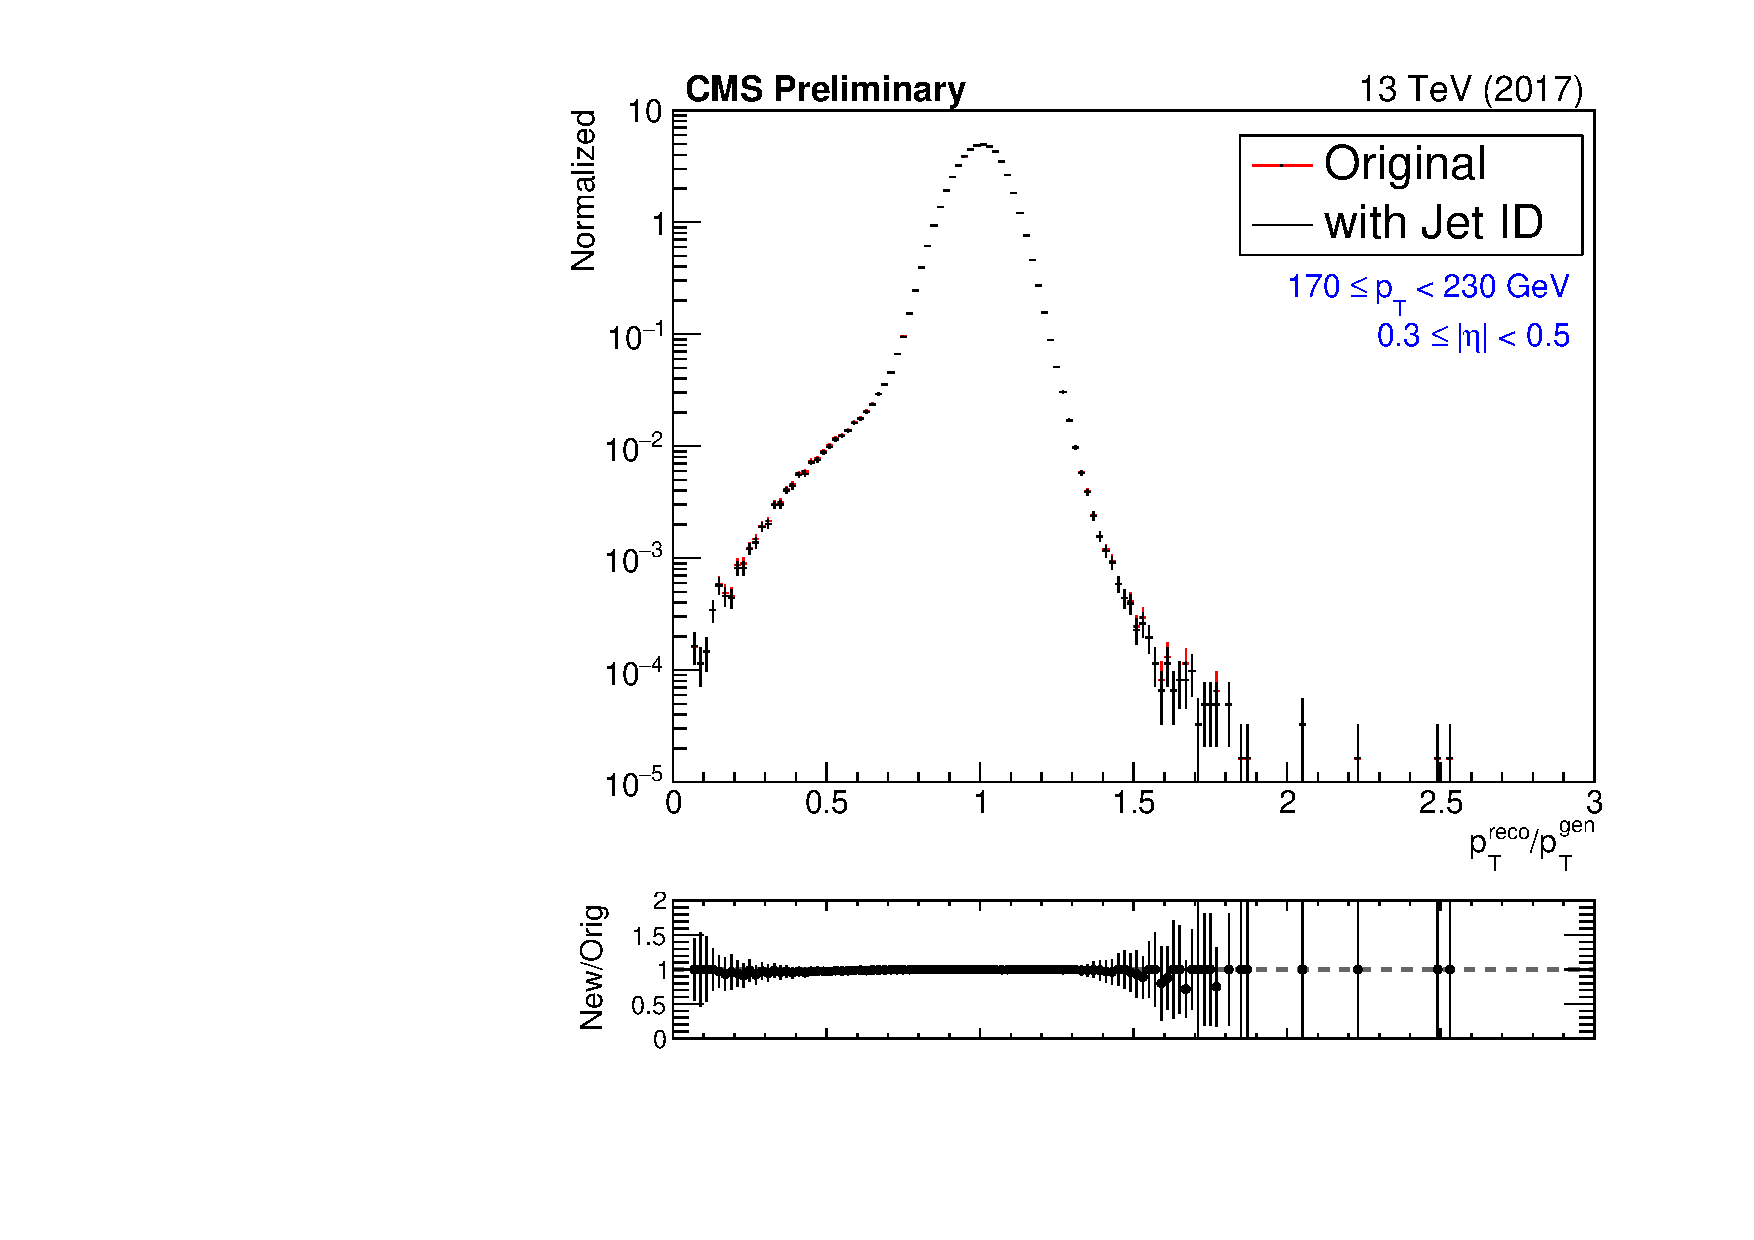
\includegraphics[width=0.325\textwidth]{figs/jetmet/compare_jetID.pdf}
    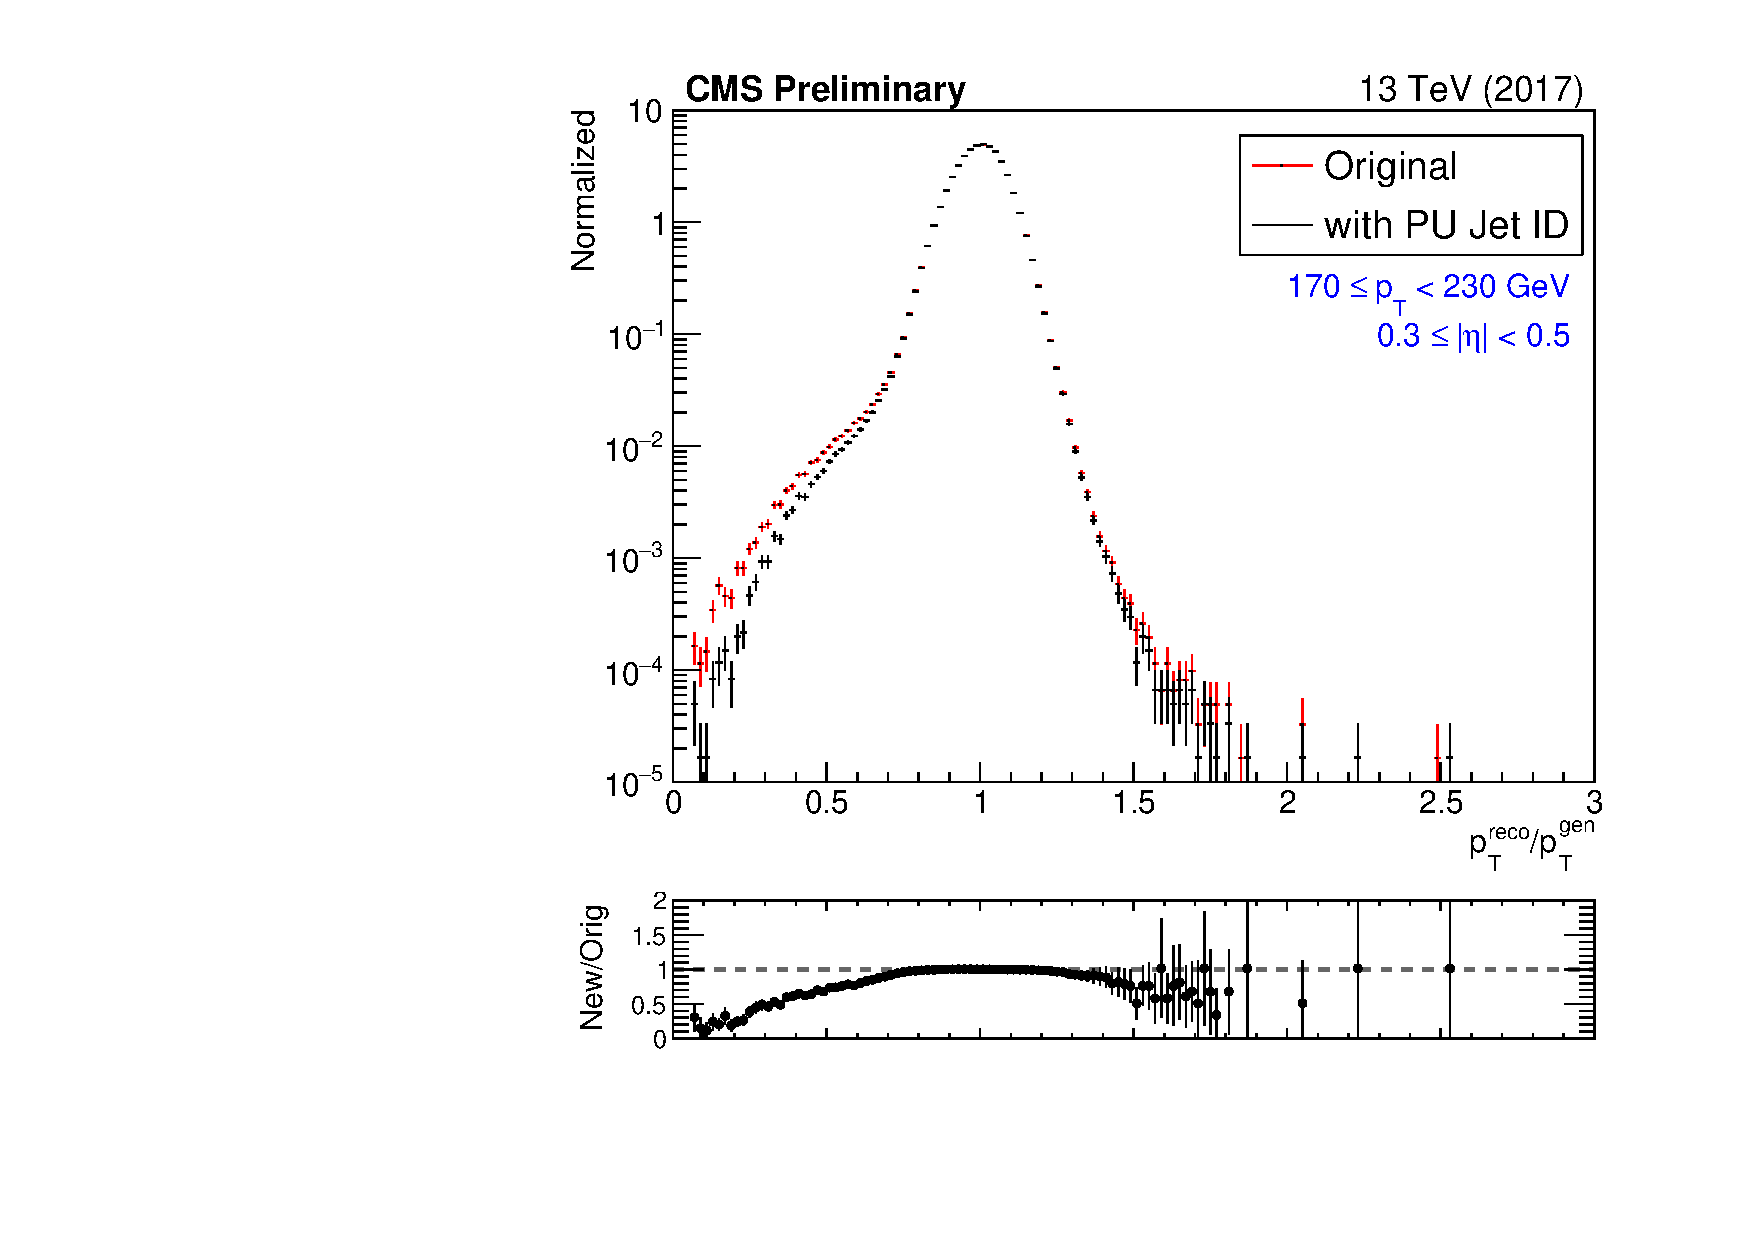
\includegraphics[width=0.325\textwidth]{figs/jetmet/compare_puJetID_highPt.pdf}
    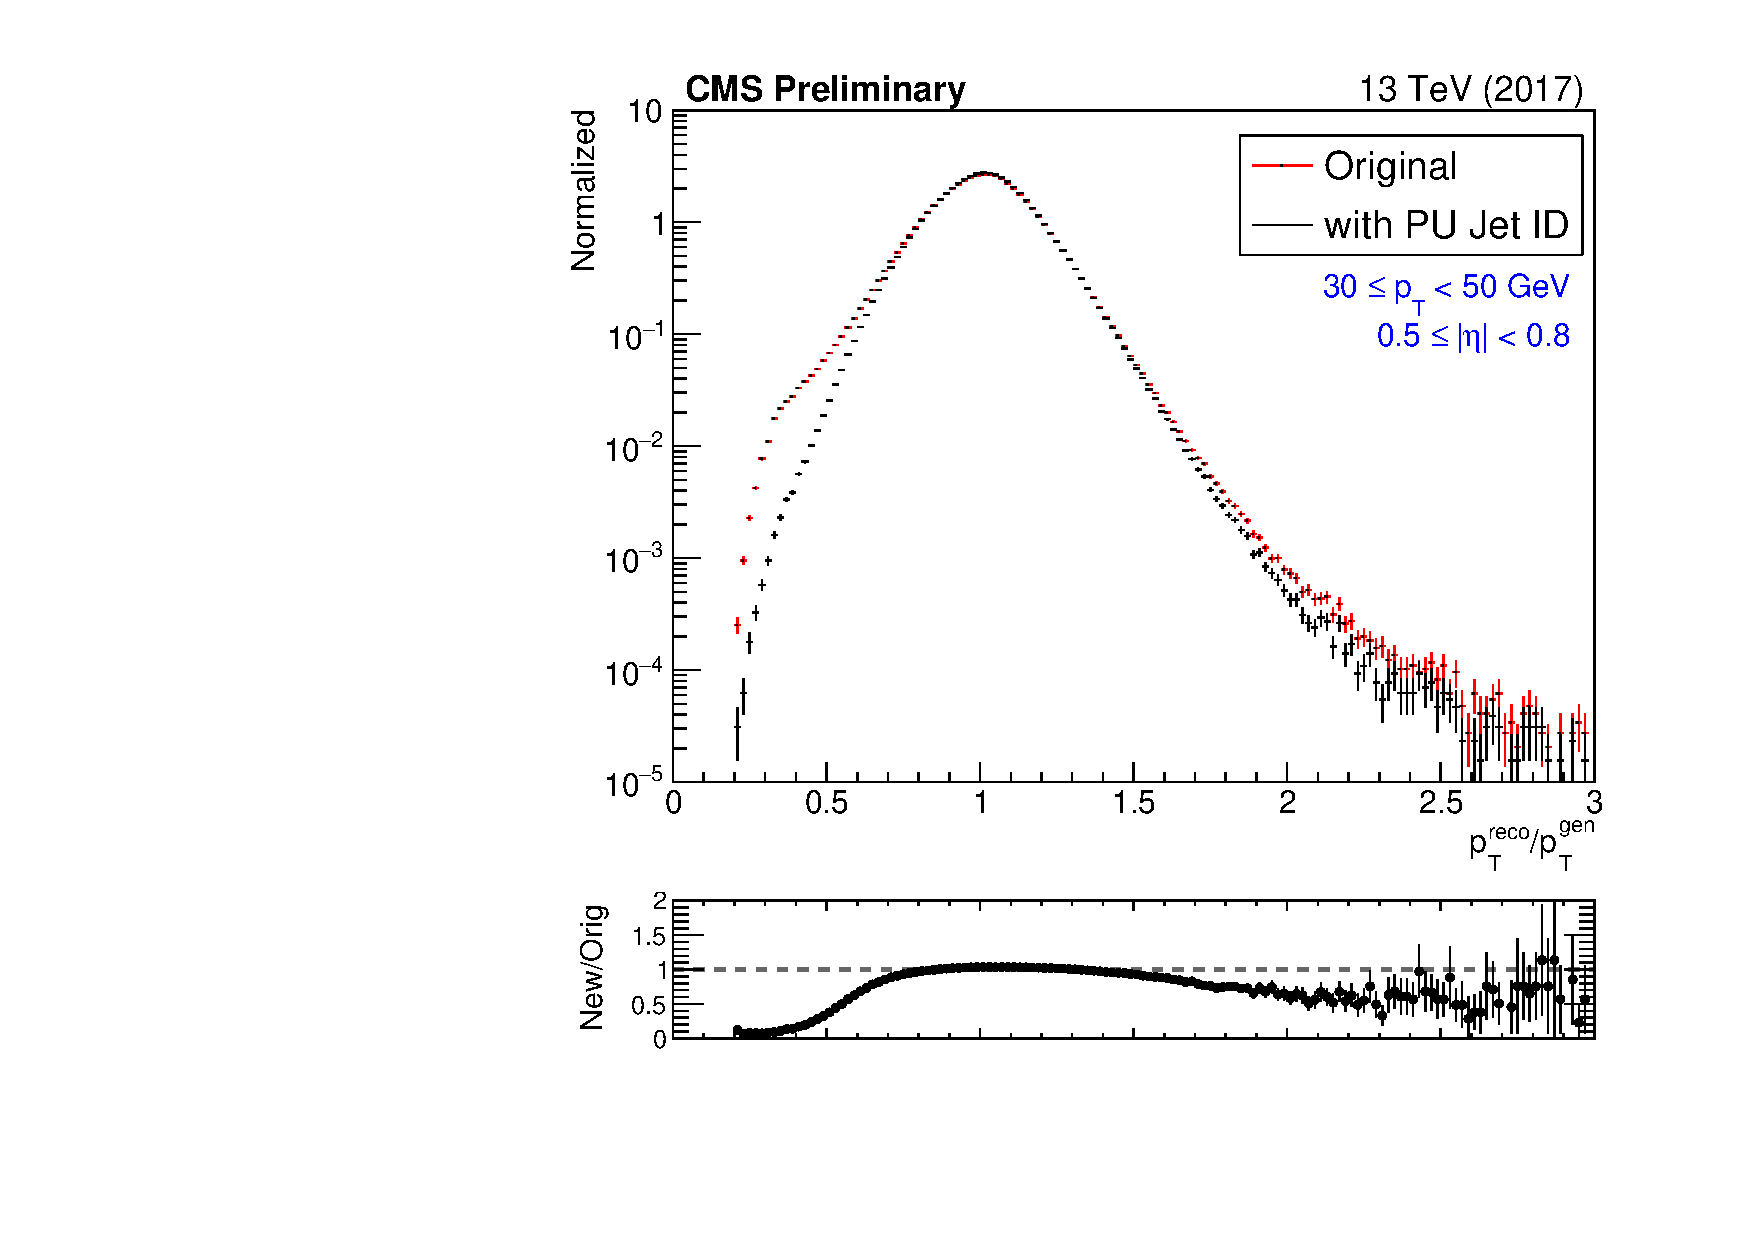
\includegraphics[width=0.325\textwidth]{figs/jetmet/compare_puJetID_lowPt.pdf}
    \caption{(left) and (center) show the effect of applying tight jet ID and loose pileup jet ID, respectively,
    to the same template as in Fig.~\ref{fig:jrt_matching_effect}. Jet ID has negligible effect,
    while the pileup jet ID leads to a reduction in the left tail.
    (right) The effect of pileup jet ID on a lower \pt template ($30\leq\pt<50$ GeV). Here we observe
    a reduction in both tails.
    }
    \label{fig:jrt_jetid}
  \end{center}
\end{figure}

In the final step, we have identified jet pairs and need to fill histograms. The only thing left to decide
is how to fill the b and non-b jet templates. There are three options that have all been tried:
\begin{enumerate}
  \item Fill only a single histogram, based on the gen jet flavor (found by identifying flavor of hadrons within jet).
  \item Fill only a single histogram, based on whether the reco jet is medium b-tagged.
  \item Fill both histograms, with weights given by the probability of tagging that jet as a b jet (corrected with data/MC scale factors).
\end{enumerate}

We evaluate each method empirically by observing the agreement in \nbtags in QCD-enriched control regions after applying
the full Rebalance and Smear method described in Chapter~\ref{chap:qcd}. It is found that (2) slightly improves on (1), and (3) is quite a bit better than both.
An example of the effect is shown in Fig.~\ref{fig:jrt_nb}.

\begin{figure}[htbp]
  \begin{center}
    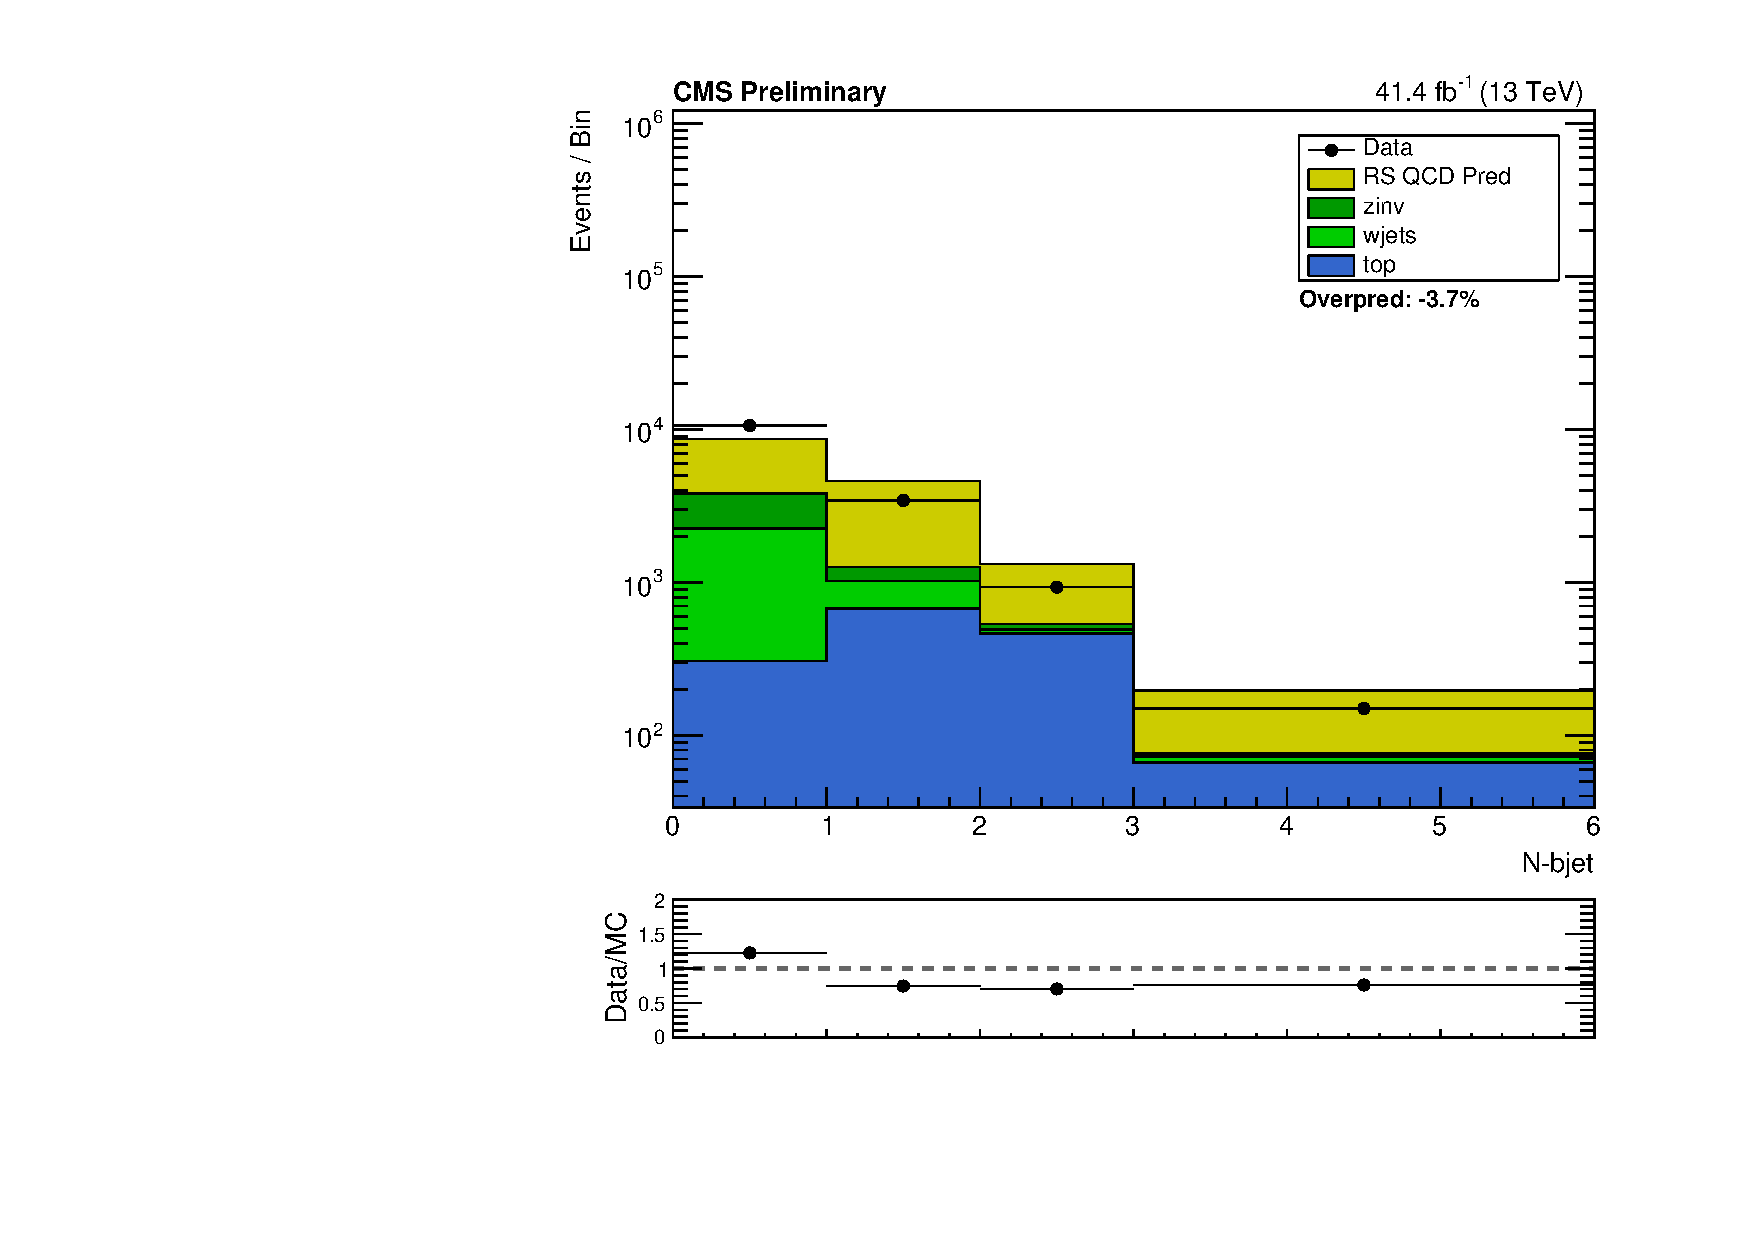
\includegraphics[width=0.49\textwidth]{figs/jetmet/nBJet20_DPhiMT2InclusiveHT450to1200_RecoBJet.pdf}
    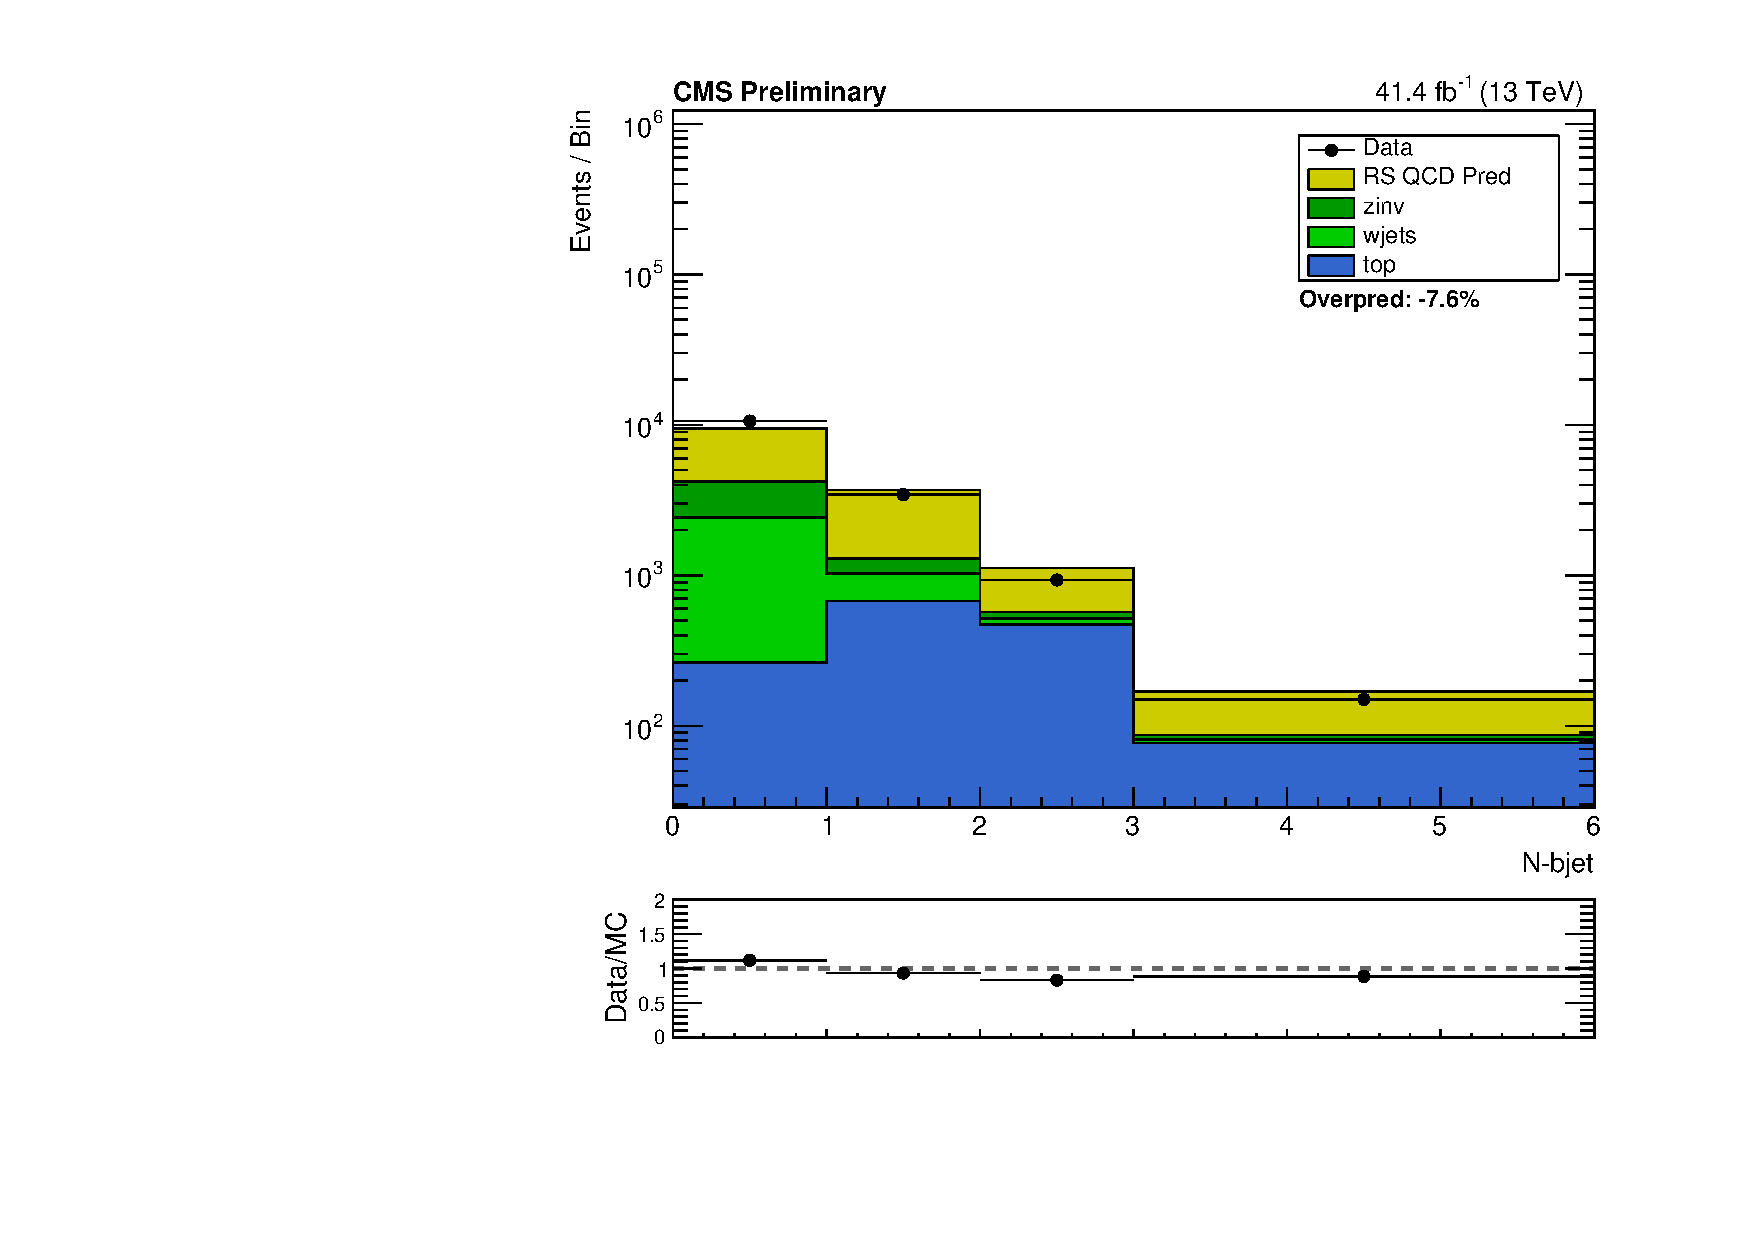
\includegraphics[width=0.49\textwidth]{figs/jetmet/nBJet20_DPhiMT2InclusiveHT450to1200_BTagSFs.pdf}
    \caption{The \nbtags distributions in the inverted-\dpmin + \mttwo sideband control region for $450 \leq \Ht < 1200$ GeV
    (described in Chapter~\ref{chap:qcd}),
    when (left) filling a single template based on reco jet medium b tagging, and (right) filling both histograms with
    weights given by the corrected probability of tagging a given jet as a medium b jet. Observed data are shown
    as black points, and prediction from the full Rebalance and Smear method is shown in yellow.
    Significant improvement is seen when using the second method. Residual shape discrepancies are 
    covered by a dedicated \nbtags shape systematic in the final estimate.
    }
    \label{fig:jrt_nb}
  \end{center}
\end{figure}


\subsection{Fits and jet energy resolution corrections}
\label{sec:jrt_fits}

Once the templates are derived, it is useful to split each template into a gaussian ``core'' and
non-gaussian ``tails'' The reason for this is twofold. First, it is known that jet resolution
is slightly different in data than in MC. This only applies to the standard gaussian smearing of the jets,
so in order to correct for the differences the gaussian core must be isolated.
Second, is is useful for studies on systematics to be able to alter the core/tails of the
templates individually. For example, to study the effect of mis-modeling in the tails,
one should be able to modify the size of the tails without affecting the size/shape
of the gaussian core.

To fit the core of a template, a gaussian is fitted in the range (mean $\pm$ RMS), where mean and RMS
are the mean and standard deviation of the template.
When measuring jet energy resolution and deriving scale factors, CMS only defines the core
of the jet response function as extending out to $\pm2\sigma$ of the fitted gaussian~\cite{JME_jes_jer}.
To be consistent, we use the same definition here, and in order to avoid discontinuities,
we linearly scale the gaussian to 0 between $\pm1$ and 2 $\sigma$. Precisely, if $g(x)$ is the
full fitted gaussian, and $\mu$ and $\sigma$ are its mean and standard deviation, our defined core function is
\[
\text{Core}(x) = 
\begin{cases}
g(x) & \text{if } |x-\mu| \leq 1\sigma \\
g(x)\left(2-\frac{|x-\mu|}{\sigma}\right) & \text{if } 1\sigma < |x-\mu| \leq 2\sigma \\
0 & \text{if } |x-\mu| > 2\sigma \\
\end{cases}.
\]

The tails are then simply defined as the full template function minus $\text{Core}(x)$.
Examples of this fitting procedure are shown in Fig.~\ref{fig:jrt_examples}. The truncated-gaussian
cores are shown in red, and the tails in green.

The first way that these fits are used is in the correction of the templates for jet energy resolution
differences between data and MC. The JetMET group provides year-dependent scale factors binned in 
$\eta$, shown in Table~\ref{tab:jrt_jersfs}. When smearing data events, the core of the template for a given jet
is widened by this scale factor before drawing a random smear factor from the distribution. This is done in a 
way to preserve the relative core/tail normalization. Specifically, if $\alpha$ is the scale factor by which we
want to widen the core, the modified template is given by
\[
f_\alpha(x) = \frac{1}{\alpha}\cdot\text{Core}((x-1)/\alpha+1) + \text{Tail}(x).
\]

\begin{table}[htp]
\caption{Jet energy resolution scale factors (data resolution divided by MC resolution) provided by the JetMET group.
             Uncertainties are statistical plus systematic.}
\label{tab:jrt_jersfs}
\centering
%\small
\begin{tabular}{|c|ccc|}
\hline
 & 2016 & 2017 & 2018 \\ \hline
$0.0 \leq |\eta| < 0.5$ & $1.160\pm0.065$ & $1.143\pm0.022$ & $1.150\pm0.042$ \\
$0.5 \leq |\eta| < 0.8$ & $1.195\pm0.065$ & $1.182\pm0.048$ & $1.134\pm0.080$ \\
$0.8 \leq |\eta| < 1.1$ & $1.146\pm0.063$ & $1.099\pm0.046$ & $1.102\pm0.052$ \\
$1.1 \leq |\eta| < 1.3$ & $1.161\pm0.103$ & $1.114\pm0.140$ & $1.134\pm0.112$ \\
$1.3 \leq |\eta| < 1.7$ & $1.128\pm0.099$ & $1.131\pm0.147$ & $1.104\pm0.211$ \\
$1.7 \leq |\eta| < 1.9$ & $1.100\pm0.108$ & $1.160\pm0.097$ & $1.149\pm0.159$ \\
$1.9 \leq |\eta| < 2.1$ & $1.143\pm0.121$ & $1.239\pm0.191$ & $1.148\pm0.209$ \\
$2.1 \leq |\eta| < 2.3$ & $1.151\pm0.114$ & $1.260\pm0.150$ & $1.114\pm0.191$ \\
$2.3 \leq |\eta| < 2.5$ & $1.296\pm0.237$ & $1.409\pm0.202$ & $1.347\pm0.274$ \\
$2.5 \leq |\eta| < 2.8$ & $1.342\pm0.209$ & $1.991\pm0.568$ & $2.137\pm0.524$ \\
$2.8 \leq |\eta| < 3.0$ & $1.779\pm0.201$ & $2.292\pm0.374$ & $1.650\pm0.941$ \\
$3.0 \leq |\eta| < 3.2$ & $1.187\pm0.124$ & $1.270\pm0.109$ & $1.225\pm0.194$ \\
$|\eta| \geq 3.2$       & $1.192\pm0.149$ & $1.154\pm0.152$ & $1.082\pm0.198$ \\
\hline
\end{tabular}
\end{table}

To assign a systematic from uncertainty in the jet energy resolution modeling, the smearing is run three times:
once using the central values in Table~\ref{tab:jrt_jersfs}, once with the $+1\sigma$ values,
and once with the $-1\sigma$ values. The differences in final signal region predictions,
integrated over each \Ht region, are used to assign a systematic uncertainty. The results of this
procedure are shown in Fig.~\ref{Fig:rs_data_JER_var} in Sec.~\ref{sec:app_rs_modify_core}.

The fitted tails are used in a similar way to assign a systematic due to uncertainty in the tail modeling.
The tails are not stretched along the $x$ direction, but instead simply scaled up/down (i.e., their normalization
relative to the core is increased/decreased). Formally, to increase the tail size by a factor $\beta$, the
modified template is given by
\[
   f_\beta(x) = N_\beta(\text{Core}(x) + \beta\cdot\text{Tail}(x)),
\]
where $N_\beta$ is a normalization factor to ensure that the template integral remains equal to one.
Results of applying this procedure to the smearing of QCD MC with $\beta=1.25$ and 1.50 
are shown in Fig.~\ref{Fig:rs_modify_tail} in Sec.~\ref{sec:app_rs_modify_tail}. 
The differences in final signal region yields with $\beta=1.25$ are used to assign a systematic uncertainty.

\chapter{Overview of the \texorpdfstring{$\text{M}_\text{T2}$}{MT2} Analysis}

Physics beyond the standard model at the LHC may manifest itself in a wide variety of potential final state 
topologies. Events with differing amounts of hadronic energy, missing transverse momentum, and numbers of leptons
should all be searched for signs of new physics. In this dissertation, we focus on the ``all-hadronic'' final state,
which encompasses events with no prompt leptons and large amounts of hadronic enegy and missing transverse momentum.
Section~\ref{sec:motivation} discusses the theoretical motivation for an all-hadronic search, Sec.~\ref{sec:mt2_backgrounds}
describes the various backgrounds for such a search, and Sec.~\ref{sec:mt2_variable} introduces \mttwo, a \ptmiss-based kinematic
variable that is used to discriminate signal from background.

\section{Motivation for an all-hadronic search}
\label{sec:motivation}

Many theories of BSM physics contain heavy particles (masses on the order of hundreds of GeV to TeV), whose
decays produce a multitude of highly energetic particles. Thus, the events tend to have lots of visible
energy (in the form of highly energetic jets and/or leptons) as well as
\emph{invisible} energy (in the form of \ptmiss), if the decay products are not detectable.

Most SM processes that produce significant true \ptmiss from neutrinos also have leptons, since the
neutrinos often come from $W\to\ell\nu$ decay. This is especially true for events with many jets
and b-tagged jets, which often contain a \ttbar pair. So by vetoing events with prompt leptons, it is
possible to significantly reduce a large class of SM backgrounds. The flip side of this is that a
zero-lepton selection will be contaminated by events from QCD multijet production, with significant
fake \ptmiss from jet mis-measurement. However, this can be managed with the use of a variety of
discriminating kinematic variables, discussed in Sec.~\ref{sec:mt2_variable} and Chapter~\ref{chap:event_selection}.

Based on general concerns, then, there is motivation for a search with lots of hadronic energy and
missing transverse momentum, but no leptons. There are also many specific examples of models
of BSM physics that produce such final states. Decay chains in simplified models of supersymmetry, discussed in
Sec.~\ref{sec:susy}, are often completely hadronic. Two examples are shown in Fig.~\ref{fig:example_susy_feyn}.
The left diagram shows the pair production of two gluinos, each decaying to a \ttbar pair and an invisible \lsp.
Each top quark then has a 68\% probability of decaying purely hadronically. The right diagram shows
the pair production of bottom squarks, each of which decay to a bottom quark and \lsp.

\begin{figure}[t]
  \begin{center}
    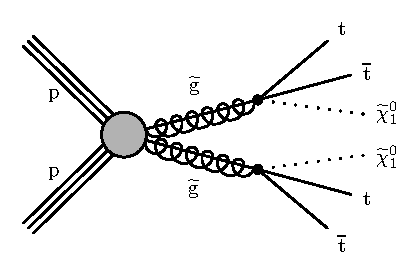
\includegraphics[width=0.40\textwidth]{figs/susy_diagrams/T1tttt.pdf}
    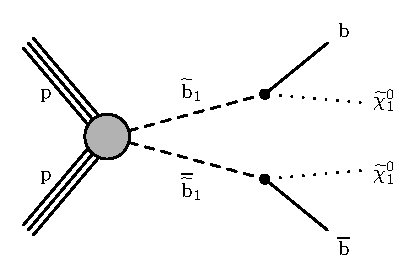
\includegraphics[width=0.40\textwidth]{figs/susy_diagrams/T2bb.pdf}
    \caption{Example Feynman diagrams of strongly-produced SUSY particles decaying hadronically.
      (left) Gluino pair production, where each gluino decays into a neutralino and two top quarks.
      (right) Bottom squark pair production, where each squark decays into a neutralino and bottom quark.
            }
    \label{fig:example_susy_feyn}
  \end{center}
\end{figure}

Additionally, the pair production of leptoquarks, discussed in Sec.~\ref{sec:leptoquarks}, may produce purely hadronic final
states if each leptoquark decays into a quark and neutrino (e.g., $\mrm{LQ}\to t\bar{\nu}_\tau$). In the case that the
leptoquarks are scalars (spin 0), this process is indistinguishable from the pair production of squarks that decay to a quark 
and \lsp when $m_\lsp=0$, so any analysis optimized to search for hadronically-decaying squark pairs is naturally optimized
to search for leptoquark pairs.


\section{Sources of backgrounds}
\label{sec:mt2_backgrounds}

The \mttwo analysis targets new physics signatures in all-hadronic events with large amounts of missing transverse momentum.
This selection leads to backgrounds that fall into three main categories:
\begin{enumerate}
\item \textbf{Invisible Z}: \znunu events produced in associated with jets contain genuine \ptmiss, and represent
an \emph{irriducible} background to the analysis. While there is no real handle to eliminate these events, as they
look exactly like signal, the events contain no inherent b-jets so the background becomes less important in
signal regions with large numbers of b-tagged jets. This background is estimated using \zll events,
as described in Chapter~\ref{chap:zinv}.
\item \textbf{Lost lepton}: events with leptonically-decaying $W$ bosons contain genuine \ptmiss from the neutrino, 
but are largely rejected based on the presence of the charged lepton.
However, they can populate the signal regions if the lepton is in some way ``lost'' (usually, if it is outside of detector acceptance,
or it isn't isolated). The primary processes making up this background are \ttbar and \wjets (\ttbar is more important in regions
with b-tagged jets), but there are also minor contributions from rarer processes such as single top, $\ttbar Z$, $\ttbar W$,
$\ttbar H$, and $tt\bar{t}\bar{t}$. These are combined with \ttbar and referred to as ``top'' in the plots and tables in this
dissertation. The lost lepton background is primarily estimated with a single-lepton control sample, as described in
Chapter~\ref{chap:lostlep}.
\item \textbf{QCD multijet}: the process with by far the largest cross section at the LHC is the QCD production of
multijet events. These events have no genuine \ptmiss, but can enter high-\ptmiss signal regions if one or more
jets is mis-measured. There are a number of handles that can be used to reject these events, such as the $\Delta\phi$
between the jets and \vMet vector, and the \mttwo variable described in the next section. The remaining background
is estimated through a data-driven procedure known as ``Rebalance and Smear'', detailed in Chapter~\ref{chap:qcd}.
\end{enumerate}

\section{The \texorpdfstring{$M_\text{T2}$}{MT2} variable}
\label{sec:mt2_variable}

Defining the \emph{transverse energy} of a particle as $E_\mrm{T}^2\equiv m^2+\pt^2$, we can define the \emph{transverse mass} of a two-particle system as
\be\label{eq:mtlong}
\begin{split}
M_\mrm{T}^2 &\equiv (E_\mrm{T,1}+E_\mrm{T,2})^2 - (\vec{p}_\mrm{T,1} + \vec{p}_\mrm{T,2})^2 \\
&= m_1^2 + m_2^2 + 2(E_\mrm{T,1}E_\mrm{T,2} - \vec{p}_\mrm{T,1}\cdot\vec{p}_\mrm{T,2}).
\end{split}
\ee

Assuming massless particles (or, equivalently, particles that are highly relativistic such that $E\gg m$ and $E_\mrm{T}\approx\pt$), this simplifies to
\be\label{eq:mt}
M_\mrm{T}^2 = 2p_\mrm{T,1}p_\mrm{T,2}(1-\cos\theta),
\ee
where $\theta$ is the angle between the particle transverse momentum vectors.

This variable is frequently useful when a particle decays to something visible and something invisible (e.g. $W\to e\nu$).
Assuming that the invisible particle is the dominant source of missing energy in the event, the \vMet vector is approximately the
transverse momentum vector of the invisible particle and can be plugged into Eq.~\ref{eq:mt} to compute the transverse mass of the
system. As the transverse mass is just the invariant mass computed only with the transverse components of the particle momenta,
it naturally has an upper bound equal to the parent particle mass. An example from a CMS measurement of the $W$ production
cross section \cite{CMS:w_prod} is shown in Fig.~\ref{fig:w_transverse_mass}. In this case, the two-particle system is
$W\to\mu\nu$ decay, and $M_\mrm{T}\lessapprox M_W=80\GeV$. The location of the $M_\mrm{T}$ ``cliff'' can be used to
extract a measurement of the $W$ mass. The small number of events with transverse mass larger than the $W$ mass
are due to experimental resolution on the muon momentum and \vMet vectors.

\begin{figure}[t]
  \begin{center}
    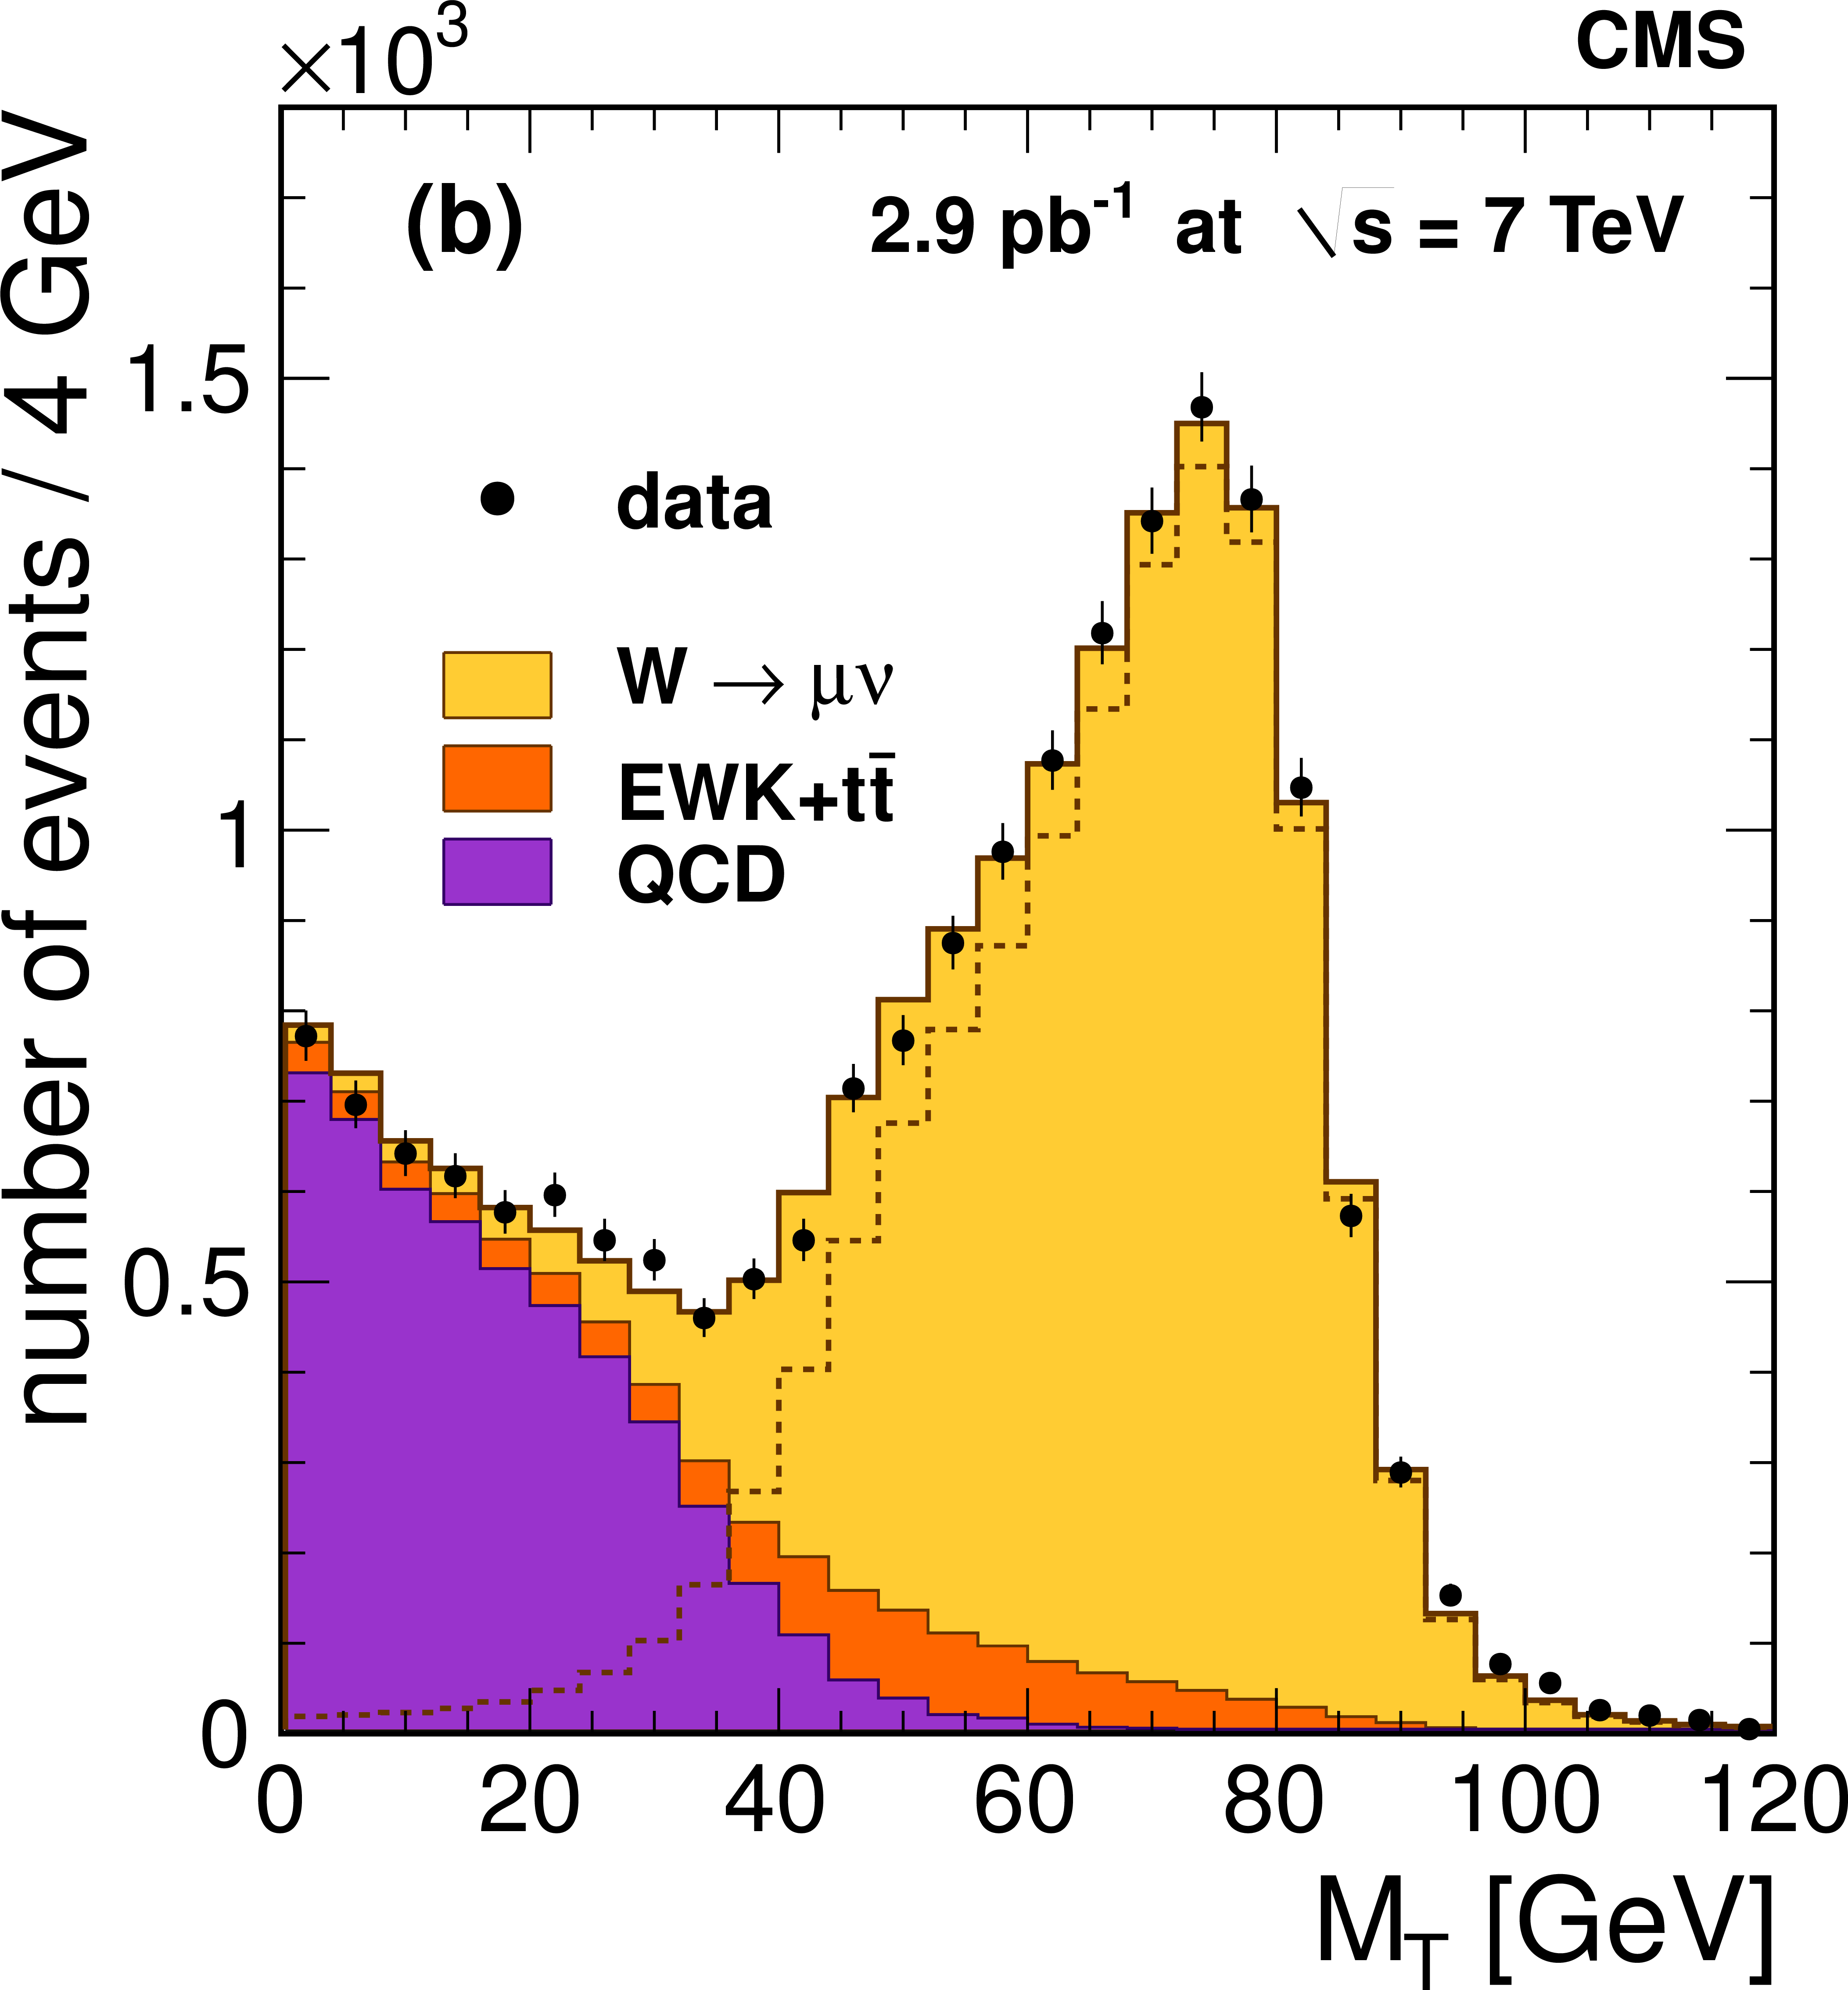
\includegraphics[width=0.45\textwidth]{figs/overview_mt2/w_transverse_mass.png}
    \caption{Transverse mass of the muon-\vMet system from a CMS measurement of the $W$ production cross section \cite{CMS:w_prod}.
      The transverse mass has a rough upper bound at $M_W=80\GeV$, limited by experimental resolution.
            }
    \label{fig:w_transverse_mass}
  \end{center}
\end{figure}

Computing the transverse mass of a decaying SUSY particle would be useful in distinguinging signal from background, since they tend to be much heavier than
SM particles that make up the background. However, the SUSY particles are \emph{pair-produced}, and computing the transverse mass 
of each system is not possible because it is not possible to resolve the \vMet vector into components from
each invisible particle. An example of this is the SUSY bottom squark pair production shown in 
Fig.~\ref{fig:example_susy_feyn} (right). Each bottom squark decays into a b quark, which appears
as a jet in the detector (potentially b-tagged), and a neutralino, which is invisible.

Absent this information, the best we can do is to try \emph{all possible partitions} of the \vMet vector
and choose the one that gives the weakest $M_\mrm{T}$ bound. This minimized quantity should be bounded above
by the mass of the pair-produced parent particles.
So, following \cite{mt2_def} we define
\be
\mttwo = \min_{\vSS{p}{\mrm{T}}{X(1)} + \vSS{p}{\mrm{T}}{X(2)} = \vMet}
\left[\max\left(M_\mrm{T}^{(1)},M_\mrm{T}^{(2)}\right)\right],
\ee
where (from Eq.~\ref{eq:mtlong})
\be\label{eq:mti}
M_\mrm{T}^{(i)2} = m_{\mrm{vis}(i)}^2 + m_X^2 + 
2\left(E_\mrm{T}^{\mrm{vis}(i)}E_\mrm{T}^{X(i)} - \vSS{p}{\mrm{T}}{\mrm{vis}(i)}\cdot\vSS{p}{\mrm{T}}{X(i)}\right)
\;\;(i=1,2),
\ee
vis$(i)$ represents the $i^\mrm{th}$ ``visible'' system, $E_\mrm{T}^{X(i)}$ and $\vSS{p}{\mrm{T}}{X(i)}$ are the assigned transverse energy and momentum of each invisible particle, 
and $m_X$ is the mass of the invisible particle. The maximum of $M_\mrm{T}^{(1)},M_\mrm{T}^{(2)}$ is used, since if
the correct momenta are chosen then \emph{both} should be bounded above by the parent mass.

A couple of complications arise when trying to practically implement this. First, there are typically more than two visible objects
in an event (either the event is accompanied by ISR or pileup jets, or the decay cascade natrually produces more than one visible
object. For example, gluino decay into top quarks, illustrated in Fig.~\ref{fig:example_susy_feyn} (left), produces multiple jets per
decaying gluino). If the original pair-produced particles are produced back-to back, the visible systems tend to be in opposite
hemispheres. So before computing \mttwo, all jets in the event are clustered into two \emph{pseudojets} following the algorithm
described in Ref.~\cite{CMS:tdr}, Section 13.4, and these pseudojets are used as the two visible systems. 
First, two initial seed axes are chosen. In this analysis they are chosen
by identifying the two jets that have the largest dijet invariant mass. Next, other jets are associated to one of these axes
according to a clustering criterion. Here we use the minimal Lund distance, meaning that jet $k$ is associated to hemisphere
$i$ rather than hemisphere $j$ if
\be
(E_i-p_i\cos\theta_{ik})\frac{E_i}{(E_i+E_k)^2} < (E_j-p_j\cos\theta_{jk})\frac{E_j}{(E_j+E_k)^2},
\ee
where $E_i$ and $p_i$ are the energy and momentum of pseudojet $i$, and $\theta_{ik}$ is the angle between pseudojet $i$ and jet $k$.
After all jets are associated to one or the other axis, the axes are recalculated as the sum of the
momenta of all jets connected to a hemisphere. The association is iterated using these new axes
until no jets switch from one group to the other.

A second complication arises in choosing the mass terms in Eq.~\ref{eq:mti}. Computing the masses of
the two pseudojets ($m_{\mrm{vis}(i)}$) is possible, but mis-measured multijet events with large pseudojet masses
may give rise to large \mttwo, eliminating some of the discriminating power of the variable. Setting
these pseudojet masses to 0 is found to further suppress multijet events while maintaining signal sensitivity.
The invisible particle mass, $m_X$, on the contrary is an unknown parameter and could not be set to its
proper value even if desired. It is found that setting $m_X=0$ is sufficient in maintaining discriminating power.
Hence, in this analysis both mass terms in Eq.~\ref{eq:mti} are set to 0 when computing \mttwo.

As discussed in Sec.~\ref{sec:mt2_backgrounds}, a big challenge in hadronic searches is the huge cross section
for QCD production of multijet events at the LHC. While requiring large \ptmiss suppresses much of this, there is still
a large contribution from events with \ptmiss from mis-measured jets. The \mttwo variable allows further suppression
of these events, by taking advantage of the different event topologies between signal and mis-measured multijet events.

This is illustrated in Figs.~\ref{fig:inclusive_mt2} and \ref{fig:metmt2}.
Fig.~\ref{fig:inclusive_mt2} shows distributions of \mttwo for signal and background after an inclusive selection,
while Fig.~\ref{fig:metmt2} shows 2D distributions of \mttwo vs. \ptmiss separately for signal and QCD multijet events.
In SUSY events, the large mass scale of the produced sparticles and acoplanarity of the visible objects tends to concentrate
the events in the high-\mttwo region (\mttwo follows \ptmiss quite closely). On the contrary, mis-measured multijet events
populate the low-\mttwo region regardless of \ptmiss or jet \pt, since they tend to be ``back-to-back''.
Electroweak backgrounds have larger \mttwo tails than does QCD, since they contain real missing energy from neutrinos.
Because of this, after requiring high \mttwo, QCD multijet events become a sub-dominant background in all signal regions.


\begin{figure}[ht]
  \begin{center}
    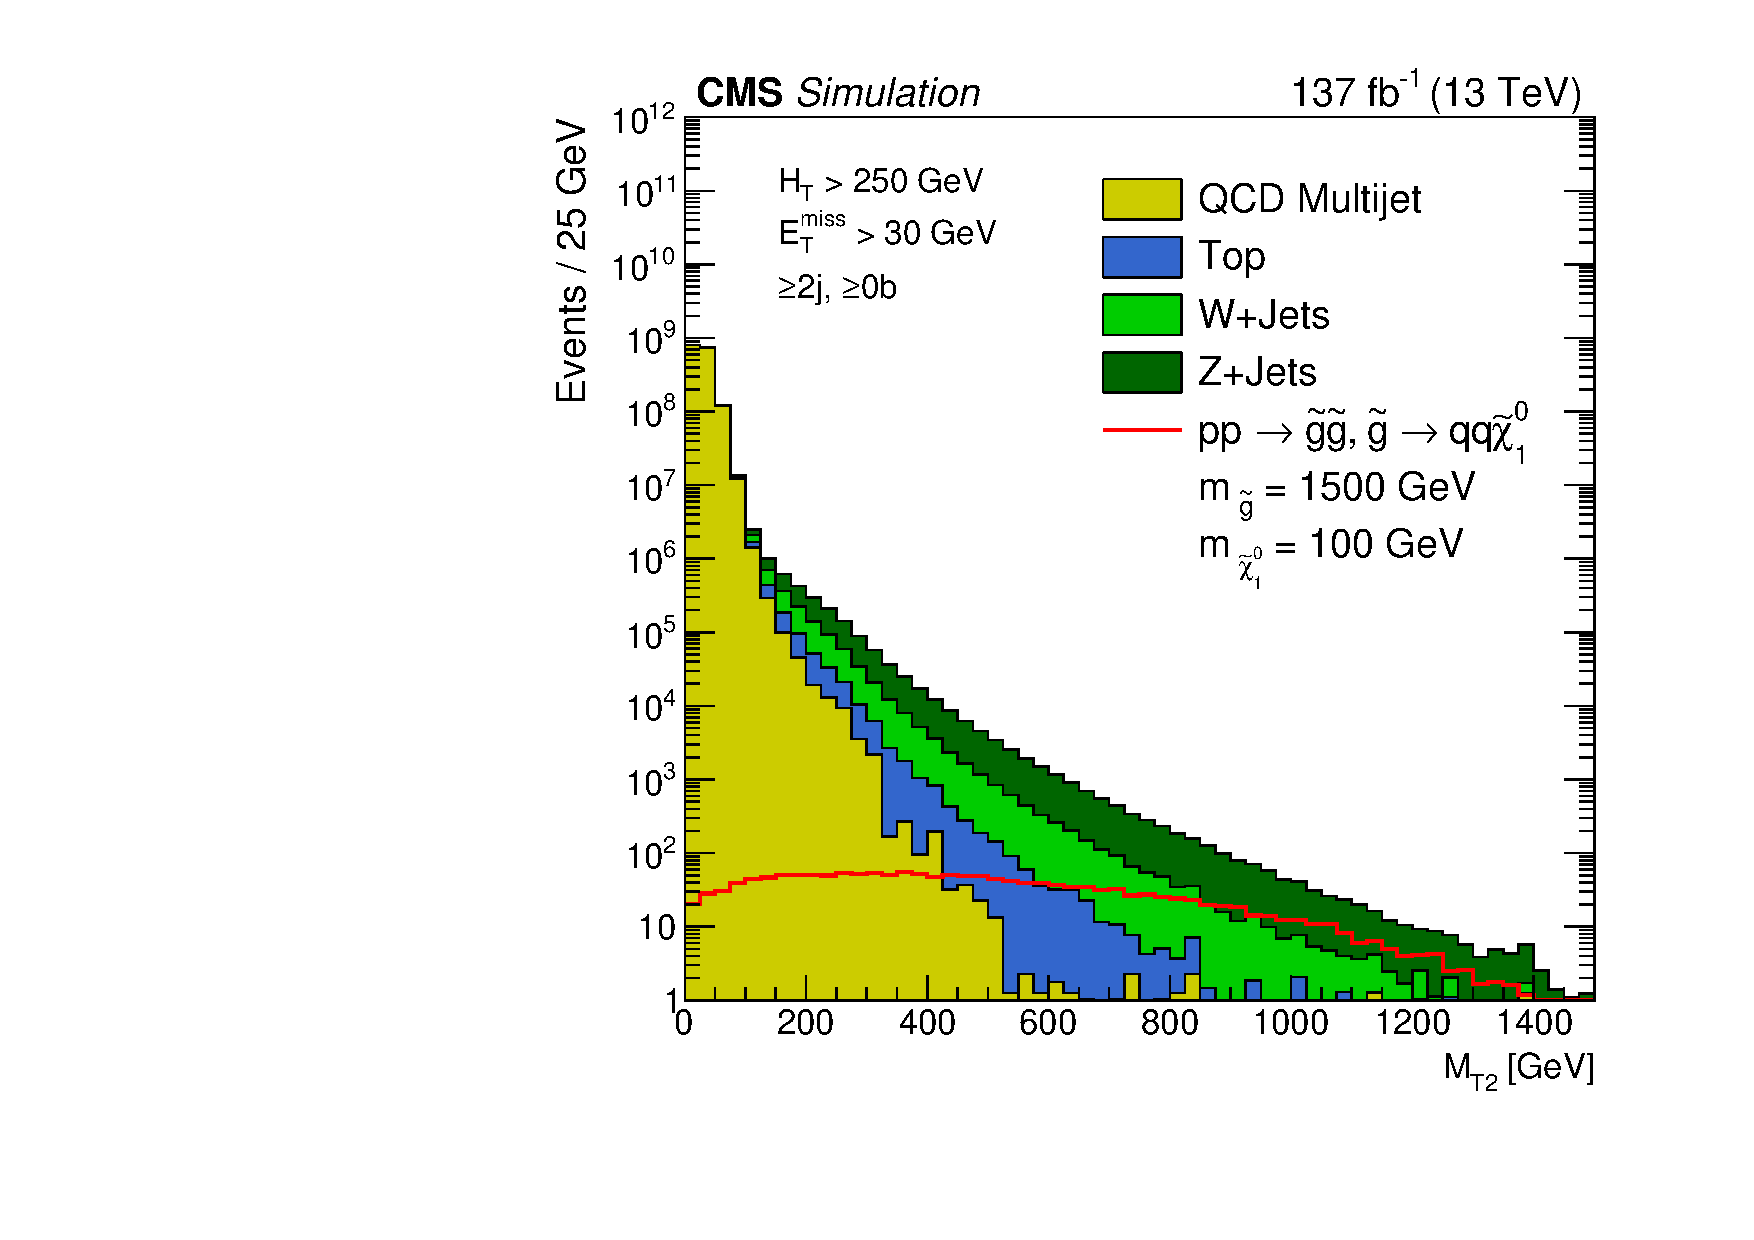
\includegraphics[width=0.50\textwidth]{figs/overview_mt2/inclusive_mt2.pdf}
    \caption{\mttwo distributions for an example signal and backgrounds after an inclusive selection of $\Ht>250\GeV$, $\ptmiss>30\GeV$, and $\Nj\geq2$.
      The signal shown is gluino pair production where each gluino decays to two light-flavor quarks and a neutralino, with 
      $m_\gluino=1500\GeV$ and $m_\lsp=100\GeV$.
      The QCD multijet background falls rapidly with \mttwo, while signal extends out to large values. The electroweak backgrounds
      have larger tails, since they containt true \ptmiss, but some discriminating power remains.
            }
    \label{fig:inclusive_mt2}
  \end{center}
\end{figure}

\begin{figure}[ht]
  \begin{center}
    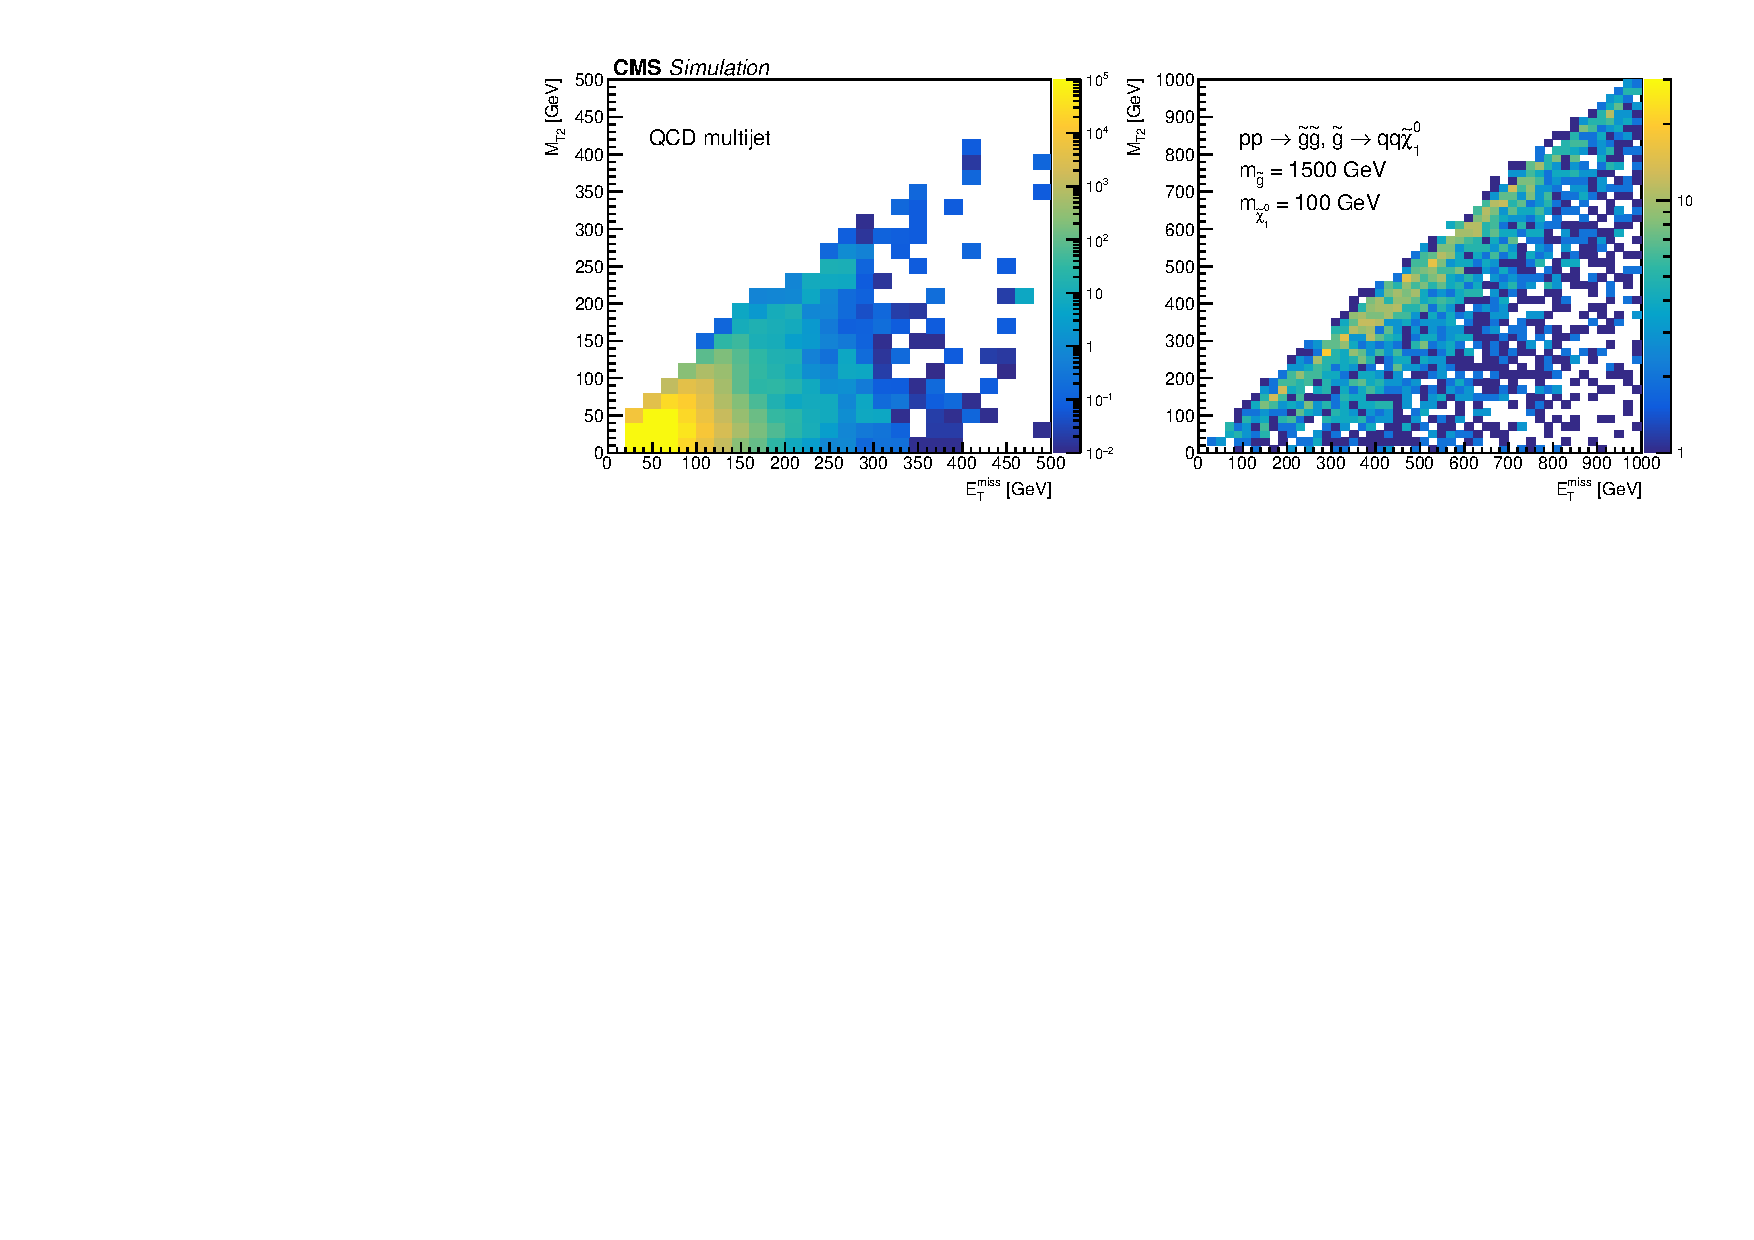
\includegraphics[width=0.98\textwidth]{figs/overview_mt2/metmt2.pdf}
    \caption{Distributions of \mttwo vs. \ptmiss, for QCD multijet events (left), and gluino pair production (right).
      For signal, $\mttwo\sim\ptmiss$, while for background, \mttwo tends to be much smaller than \ptmiss.
            }
    \label{fig:metmt2}
  \end{center}
\end{figure}

\chapter{Event Selection and Triggering}
\label{chap:event_selection}

The general strategy of the \mttwo analysis is to apply a baseline selection
motivated by the available triggers and by the desire to reduce QCD multijet
background to manageable levels, and then to categorize the selected events
into bins of differing levels of hadronic activty, number of b-tagged jets, 
and missing transverse energy. The ``namesake'' variable \mttwo, used to reduce
QCD background, was described in Sec.~\ref{sec:mt2_variable}, but a number of other
variables are also used to constrain backgrounds and categorize events.
Sec.~\ref{sec:objvardefs} defines the
relevant physics objects (jets, leptons, etc.) and kinematic variables, Sec.~\ref{sec:triggers} describes
the triggers used in the analysis, Sec.~\ref{sec:baselinesel} outlines the
baseline selection, and Sec.~\ref{sec:srdefs} gives the precise definitions
of the signal regions.

\section{Object and variable definitions}
\label{sec:objvardefs}

In CMS, individual particles are identified by combining information from the tracker, calorimeters, and muon system
using the ``particle flow'' algorithm, described in Sec.~\ref{sec:cms_det}. This particle-level information is
then used to cluster jets, reconstruct vertices, and compute the missing transverse energy. Here we list the various
physics objects used in this analysis and the selections applied on them.

\subsection{Vertices}
\label{sec:vertices}
``Vertex finding'' is a process of finding points in space from which groups of reconstructed particle tracks that, loosely,
come from the same ``interaction'', emanate. There is generally a single ``primary vertex'', where the hard interaction
took place, pileup vertices from pileup interactions, and, potentially, secondary vertices from longer-lived decaying particles
such as b hadrons. Algorithms for reconstructing vertices are described in \cite{TRK_vertexing}. For this analysis,
we consider a reconstructed vertex as good if it satisfies:
\begin{itemize}
\item not ``fake'' - if no vertices are reconstructed from tracks, a default vertex based on the beam-spot 
(luminous region produced by proton beam collision) is used, and is labeled as ``fake''.
\item $N_\mrm{dof}>4$ - $N_\mrm{dof}$ is the number of degrees of freedom in the fit of the position
of the vertex, essentially the number of tracks consistent with originating from the vertex.
\item $|z|<25$ cm - the longitudinal distance from the beam-spot.
\item $\rho<2$ cm - the distance from the beam axis.
\end{itemize}

When more than one good reconstructed vertex is found in the event, the reconstructed vertex
with the largest value of summed physics-object $\pt^2$ is taken to be the primary interaction
vertex.

\subsection{Jets}

Jets are clustered using the anti-$k_\mrm{T}$ algorithm with distance parameter $R=0.4$.
Charged hadrons from pileup interactions are identified and removed based on the ``charged hadron
subtraction'' algorithm \cite{JME_pileup_removal_algo}.
Jet energies are corrected for pileup contamination and detector response with CMS-derived
era-dependent jet energy corrections.
We select jets that satisfy $\pt>30\GeV$ and $|\eta|<2.4$, and pass PF jet loose ID (2016)
or tight ID (2017+18). For events with only one jet, we require tighter ID requirements to reject noisy jets. 
All jet ID cuts are summarized in Table~\ref{tab:jet_id}.

\begin{table}[h]
\caption{Jet ID definitions}
\label{tab:jet_id}
\centering
\begin{tabular}{l|c|c|c}
\hline
 & 2016 & 2017-18 & Monojet (all years) \\ \hline
Neutral hadron fraction & $<0.99$ & $<0.90$ & $<0.80$ \\
Neutral EM fraction & $<0.99$ & $<0.90$ & $<0.70$ \\
Number of constituents & $>1$ & $>1$ & $>1$ \\
Charged hadron fraction & $>0$ & $>0$ & $>0.05$ \\
Charged multiplicity & $>0$ & $>0$ & $>0$ \\
Charged EM fraction & $<0.99$ & -- & $<0.99$ \\
\hline
\end{tabular}
\end{table}

We define \Nj as the number of jets passing the above selections, and \Ht as 
the scalar sum of \pt values for all such jets.

Jets originating from b quarks are tagged using the DeepCSV algorithm \cite{BTV_btagging}, at the medium working point. 
For the purposes of counting the number of b-tags (\Nb), we loosen the \pt threshold for b-tagged jets to 20\GeV.
This helps to add sensitivity to compressed-spectrum signals with jets from b quarks.

\subsection{\ptmiss}
We use type 1-corrected PFMET, defined in Sec.~\ref{sec:jetmet}, using the same jet energy corrections
as applied to the jets. We additionally define \vMht as
\be
\vMht = -\sum_\mrm{jets} \vec{p}_{\mrm{T},i},
\ee
where the sum is taken over all jets passing the above requirements. The difference with respect to \vMet is that
this excludes forward or low-\pt jets and unclustered energy.

\subsection{\ptmiss filters}
\label{sec:metfilters}
In addition to real missing energy due to invisible particles, events may have some amount of ``fake \ptmiss'' due to either
detector effects or external sources (e.g. cosmic rays or beam-halo particles). We have discussed fake \ptmiss from 
standard jet mis-measurement due to stochaistic smearing in the calorimeters, but more pathological effects are also possible,
such as noisy calorimeter cells or bad track reconstructions. To eliminate as best as possible events containing such sources
of fake \ptmiss, the JetMET group at CMS recommends a set of ``\ptmiss filters'' that use features of the reconstructed
event to identify certain classes of bad events. We apply all standard recommended filters, listed here:
\begin{itemize}\setlength\itemsep{-1mm}
\item primary vertex filter
\item CSC super-tight beam halo 2016 filter (despite name, used in all 3 years)
\item HBHE noise filter
\item HBHE iso noise filter
\item EE badSC noise filter
\item ECAL dead cell trigger primitive filter
\item bad muon filter
\item ECAL bad calibration filter (2017+18 only)
\end{itemize}

There are also a few custom \ptmiss filters developed by this analysis or the CMS SUSY group that are applied to protect 
against other observed sources of fake \ptmiss.
First, we reject any event containing a jet with $\pt>30\GeV$ and $|\eta|<4.7$ which fails the PF jet loose/tight ID as described above.
Since this jet would not enter the collection used to compute \mttwo, the pseudojets would likely be imbalanced and the resulting
\mttwo biased.
This is not applied to fast simulation MC samples since the input variables are not correctly modeled, and \mttwo
is expected to already be high anyway.

Next, we require that the ratio of PFMET over caloMET (\ptmiss computed only with calorimeter deposits) is less than 5.
This was found to remove events with a bad high-\pt muon track inside a jet, which are not removed by either the lepton
vetoes or the bad muon track filter. 
Also to reduce the effect of mis-measured muons, we veto events that contain a jet with $\pt>200\GeV$ and a muon fraction
larger than 50\%, and that satisfies $|\Delta\phi(\mrm{jet},\ptmiss)| > \pi-0.4$.

To remove certain known pathological events in fast simulation MC, we remove events in such MC containing
a jet satisfying $\pt>20\GeV$, $|\eta|<2.5$, charged hadron fraction $<0.1$, and no matching generator-level jet
within $\Delta R<0.3$.

Finally, an issue with two HCAL endcap modules during 2018 data taking required the addition
of a special filter to reject events containing jets or electrons in the affected region. Details are given in
Sec.~\ref{sec:hem}.

\subsection{Electrons}
\label{sec:electrons}

While the analysis signal regions are purely hadronic, it is still necessary to define lepton candidates, 
both in order to define a lepton veto and to select events for the leptonic control regions.
Electron candidates are required to satisfy $\pt>10\GeV$ and $|\eta|<2.4$. Good electrons are identified
using cut-based ID working points developed by the EGamma group at CMS: the ``veto'' working point is used for
the signal region veto and the single lepton control region, and the ``loose'' working point is used for
the dileptonic \zll control region. The cuts are summarized in Table~\ref{tab:electron_id}, and definitions
for the various variables are listed here.
\begin{itemize}\setlength\itemsep{-1mm}
\item $\sigma_{i\eta i\eta}$ - a variable describing the width of the shower in the ECAL; computed using the 
reconstructed hits in a 5x5 seed cluster
\item $|\Delta\eta_\mrm{Seed}|$ - difference in $\eta$ between a ECAL cluster position and track direction at vertex extrapolated to ECAL
\item $|\Delta\phi_{In}|$ - difference in $\phi$ between a ECAL cluster position and track direction at vertex extrapolated to ECAL
\item $H/E$ - ratio of energy in HCAL behind ECAL cluster to the energy in the ECAL cluster
\item $|1/E-1/p|$ - tests consistency of ECAL cluster energy and track momentum
\item $|d0|$ - transverse impact parameter of the track with respect to the primary vertex
\item $|dz|$ - longitudinal impact parameter of the track with respect to the primary vertex
\item conversion veto - reject electron candidates that look like photon conversions to $e^+e^-$ pairs
\end{itemize}

\begin{table}[htbp]
\caption{Cut-based electron ID for the Veto and Loose ID working points, for electrons in the barrel (endcap).}
\label{tab:electron_id}
\scriptsize
\centering
\resizebox{\textwidth}{!}{%
\begin{tabular}{c|c|c}
\hline
&Veto ID & Loose ID \\
\hline
\hline
$\sigma_{i\eta i\eta}$ & \multirow{2}{*}{$ < 0.0126$ ($0.0457$)} & \multirow{2}{*}{$ < 0.0112$ ($0.0425$)}\\
(RecHits in 5x5 seed cluster)& &\\ 
\hline
$|\Delta\eta_\mrm{Seed}|$& $ < 0.00463$ ($0.00814$)& $ < 0.00377$ ($0.00674$) \\ 
\hline
$|\Delta\phi_{In}|$ &$ < 0.148$ ($0.19$) & $ < 0.0884$ ($0.169$) \\ 
\hline
\multirow{2}{*}{$H/E$} &  $ < 0.05+1.16/E_{\mathrm{SC}}+0.0324~\rho/E_{\mathrm{SC}}$ &$ < 0.05+1.16/E_{\mathrm{SC}}+0.0324~\rho/E_{\mathrm{SC}}$ \\
&($ < 0.05+2.54/E_{\mathrm{SC}}+0.183~\rho/E_{\mathrm{SC}}$)  & ($0.0441+2.54/E_{\mathrm{SC}}+0.183~\rho/E_{\mathrm{SC}}$)\\ 
\hline
$|\frac{1}{E} - \frac{1}{p}|$  &$ < 0.209$ ($0.132$) &$ < 0.193$ ($0.169$)\\ 
\hline
$|d0|$ (w.r.t. primary vertex) &$ < 0.2$ ($0.2$)~cm & $ < 0.2$ ($0.2$)~cm\\ 
\hline
$|dz| $(w.r.t. primary vertex)  &$ < 0.5$ ($0.5$)~cm  &$ < 0.5$ ($0.5$)~cm \\ 
\hline
\# of expected missing inner hits &$ \leq 2$ (3)&$ \leq 1$ (1)\\ 
\hline
conversion veto& yes & yes \\
\hline
\end{tabular}
}
\end{table}

In addition to the ID described above, electrons are required to be isolated. This is defined using relative
mini-PF isolation, as miniPFIso$/\pt<0.1$. ``PF isolation'' is just the sum of the \pt values of all particle-flow candidates
within a cone around the electron candidate, and the ``mini'' part means that this cone size gets smaller
with higher electron \pt. Precisely, the cone size used is
\begin{equation}
\label{eqn:miniiso}
 \Delta R =
  \begin{cases}
   0.2          & \text{if } \pt < 50\GeV \\
   10\GeV/\pt   & \text{if } 50 < \pt < 200\GeV \\
   0.05         & \text{if } \pt > 200\GeV
  \end{cases}
\end{equation}

A correction to the isolation to account for pileup contamination is applied, based on the event-level energy
density and the effective area of the electron cone.

\subsection{Muons}
\label{sec:muons}

Muon candidates are required to pass $\pt>10\GeV$ and $|\eta|<2.4$, and a loose ID selection defined as:
\begin{itemize}\setlength\itemsep{-1mm}
\item matched to a particle-flow muon
\item either a global muon (tracker+muon system) or a tracker-only muon
\item $|d0|<0.2$~cm (transverse impact parameter with respect to the primary vertex)
\item $|dz|<0.5$~cm (longitudinal impact parameter with respect to the primary vertex)
\end{itemize}

We require the muons to be isolated using the same relative mini PF isolation as used for the electrons,
this time requiring miniPFIso$/\pt<0.2$.

\subsection{Isolated tracks}
\label{sec:isotracks}

In addition to vetoing events with the reconstructed leptons described above, we further add a veto
for events with ``isolated tracks'' that weren't reconstructed as leptons, either because
they are charged hadrons or they failed some criteria to be promoted to a full reconstructed lepton.
This allows better rejection of backgrounds with hadronically decaying $\tau$ leptons (these frequently
produce isolated pions) or with isolated leptons that weren't caught be the lepton veto, without
appreciably affecting signal efficiency.
We select charged particle-flow candidates with different requirements depending on the type of candidate.

For particle-flow electrons and muons, we require them to pass $\pt>5\GeV$, $|\eta|<2.4$, $|dz|<0.1$~cm,
$|dxy|<0.2$~cm, and a track isolation cut of iso$/\pt<0.2$. The track isolation is computed as the sum
of all charged hadron particle-flow candidates with in a cone of $\Delta R<0.3$, and that satisfy 
$|dz|<0.1$~cm with respect to the primary vertex. For lepton counting, particle-flow leptons
within $\Delta R<0.01$ of selected reconstructed leptons are removed.

Charged particle-flow hadrons are required to pass $\pt>10\GeV$, $|\eta|<2.4$, $|dz|<0.1$~cm,
$|dxy|<0.2$~cm, and a track isolation cut of iso$/\pt<0.1$, computed in the same way as above.

\subsection{\dphimet}
The variable \dphimet (referred to as \dpmin in the following) is defined as the minimum $\Delta\phi$ between
\vMet and any of the four highest \pt jets in the event. For this variable only, we consider jets with
$\pt>30\GeV$ and $|\eta|<4.7$.


\section{Triggers}
\label{sec:triggers}

\subsection{Signal region triggers}
\label{sec:srtrigs}
The baseline \Ht and \ptmiss cuts used for the signal regions are constrained by the available
triggers utilized in the data-taking, which can be different from year to year. The signal
regions use an OR of various \Ht- and \ptmiss-based triggers, that cover different (but
overlapping) regions of phase space.

The exact triggers used are an OR of the following:

\noindent
\textbf{2016 data}
\vspace{-\topsep}
\begin{itemize}\setlength\itemsep{-1mm}
\item \texttt{HLT\_PFHT900} - pure-\Ht trigger; nominally turns on at 900\GeV but observed plateau near 1000\GeV.
\item \texttt{HLT\_PFJet450} - triggers on any jet with $\pt>450\GeV$. Not strictly necessary, but used anyway
to cover for any potential small inefficiency.
\item \texttt{HLT\_PFHT300\_PFMET100} - triggers on a combination of $\Ht>300\GeV$ and $\ptmiss>100\GeV$.
Again not strictly necessary, but covers for any potential inefficiency of the \pt miss triggers in the 
intermediate \Ht regions.
\item \texttt{HLT\_PFMET[NoMu]120\_PFMHT[NoMu]120\_IDTight} - a pure \ptmiss trigger, where the \ptmiss
is computed either with or without muons. Observed plateau around $\ptmiss=250\GeV$.
\end{itemize}

\noindent
\textbf{2017+18 data} (similar triggers to 2016, but with raised thresholds)
\vspace{-\topsep}
\begin{itemize}\setlength\itemsep{-1mm}
\item \texttt{HLT\_PFHT1050}
\item \texttt{HLT\_PFJet500}
\item \texttt{HLT\_PFHT800\_PFMET75\_PFMHT75} OR \texttt{HLT\_PFHT500\_PFMET100\_PFMHT100}
\item \texttt{HLT\_PFMET[NoMu]120\_PFMHT[NoMu]120\_PFHT60\_IDTight}
\end{itemize}

An illustration of the trigger coverage in the baseline signal region (defined in Sec.~\ref{sec:baselinesel})
is shown in Fig.~\ref{fig:trig_diagram}. At low \Ht, the only available trigger is the pure-\ptmiss trigger,
which necessetates the \ptmiss cut of 250\GeV. At higher \Ht ($>$1200\GeV), the pure-\Ht trigger can be used
and allows for the relaxing of the \ptmiss cut to 30\GeV. The \Ht+\ptmiss triggers (and jet \pt trigger)
provide redundancy in the intermediate to high \Ht regions.

\begin{figure}[ht]
  \begin{center}
    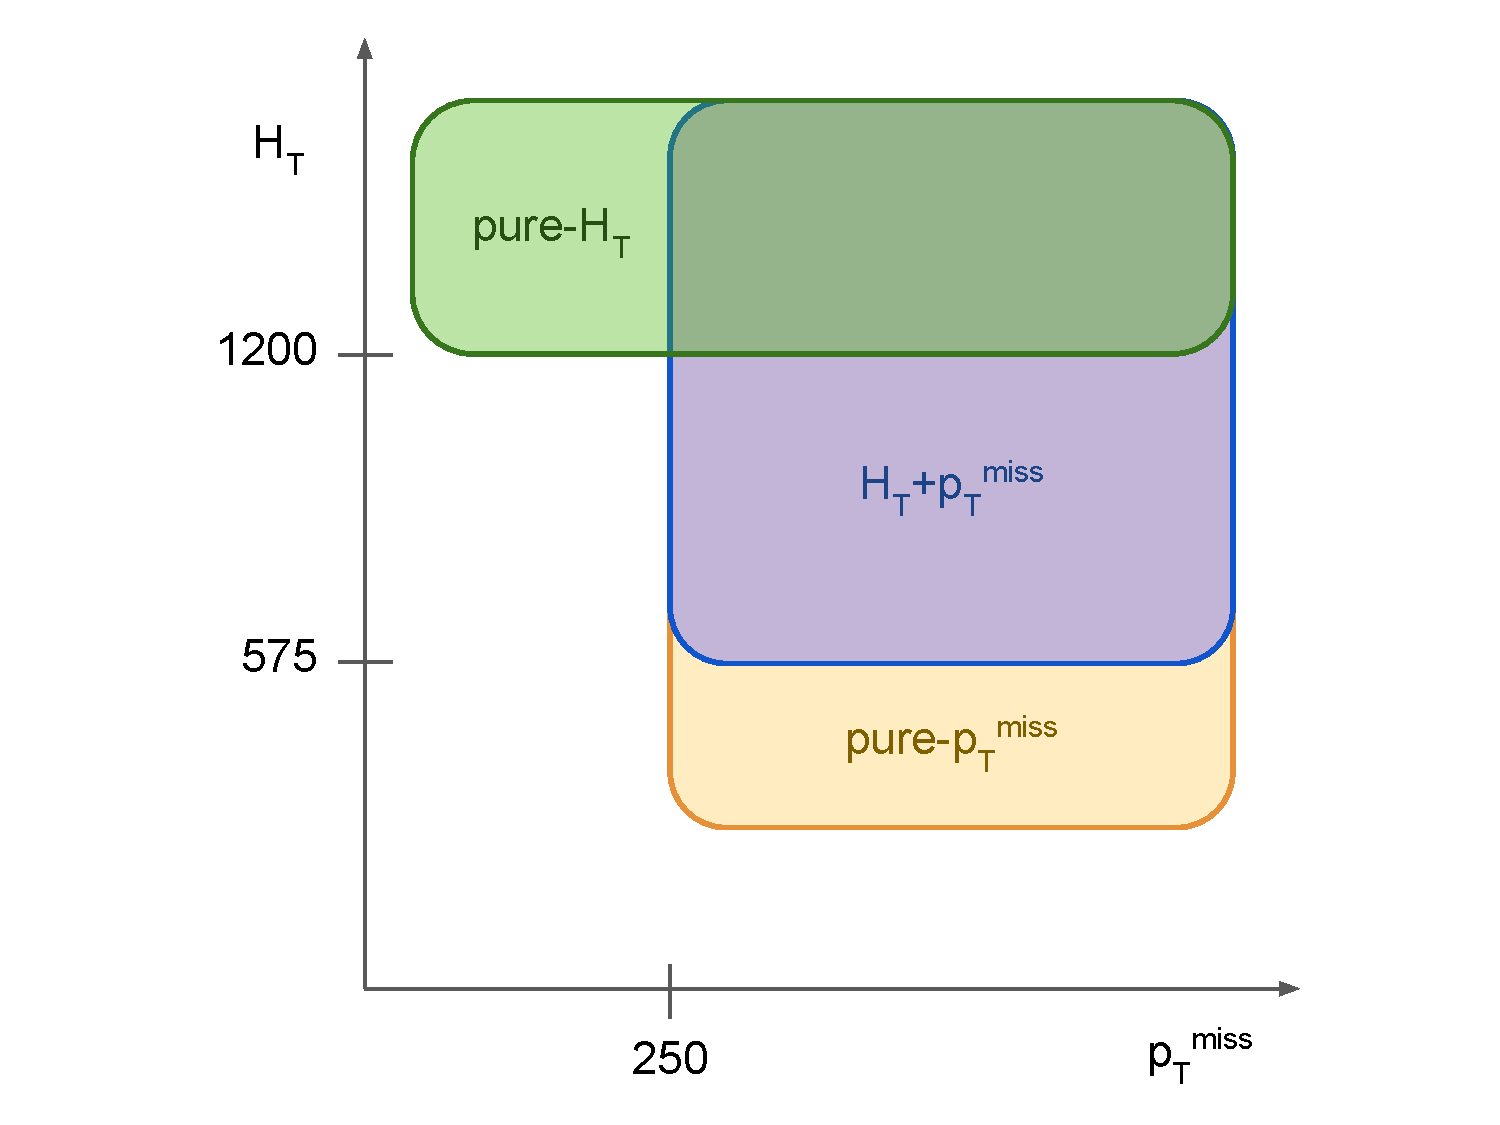
\includegraphics[width=0.65\textwidth]{figs/event_selection/trig_diagram.pdf}
    \caption{Illustration of the trigger coverage of the baseline signal region (defined in Sec.~\ref{sec:baselinesel}).
      The pure-\ptmiss triggers cover the low-\Ht regions, starting at $\ptmiss=250\GeV$.
      The pure-\Ht trigger covers the high-\Ht regions, starting at $\Ht=1200\GeV$.
      The \Ht+\ptmiss triggers provide redundancy and cover for any
      small inefficiencies in the intermediate \Ht regions.
            }
    \label{fig:trig_diagram}
  \end{center}
\end{figure}

Measuring the efficiency of the triggers is imporant to ensure the signal regions are fully covered and trigger
at near 100\%. To make this measurement, a selection in the plateau of an orthogonal ``reference trigger''
is made, and then the efficiency of the desired trigger is plotted as a function of the relevant kinematic
variable. 

The efficiency of the pure-\Ht triggers is measured in two ways: one using an electron trigger
reference, and one using a \ptmiss trigger reference. Both methods start by selecting events that pass
all \ptmiss filter, and that have at least 2 jets with $\pt>30\GeV$ and no leptons (other than the 
potential reference electron). The electron method further requires
that the event passes a single electron trigger, and contains an electron with $\pt>35\GeV$ that is 
isolated and passes a tight cut-based ID. The \ptmiss method requires that the event passes the
pure-\ptmiss trigger and has $\ptmiss>300\GeV$. Both methods give consistent results, with 
pleateau efficiencies of $>$98\%. After combining with the \texttt{HLT\_PFJetXXX} trigger,
the efficiency is $>$99\% in all years. Example measurements are shown in Fig.~\ref{fig:trigmeas_HT}.

\begin{figure}[ht]
  \begin{center}
    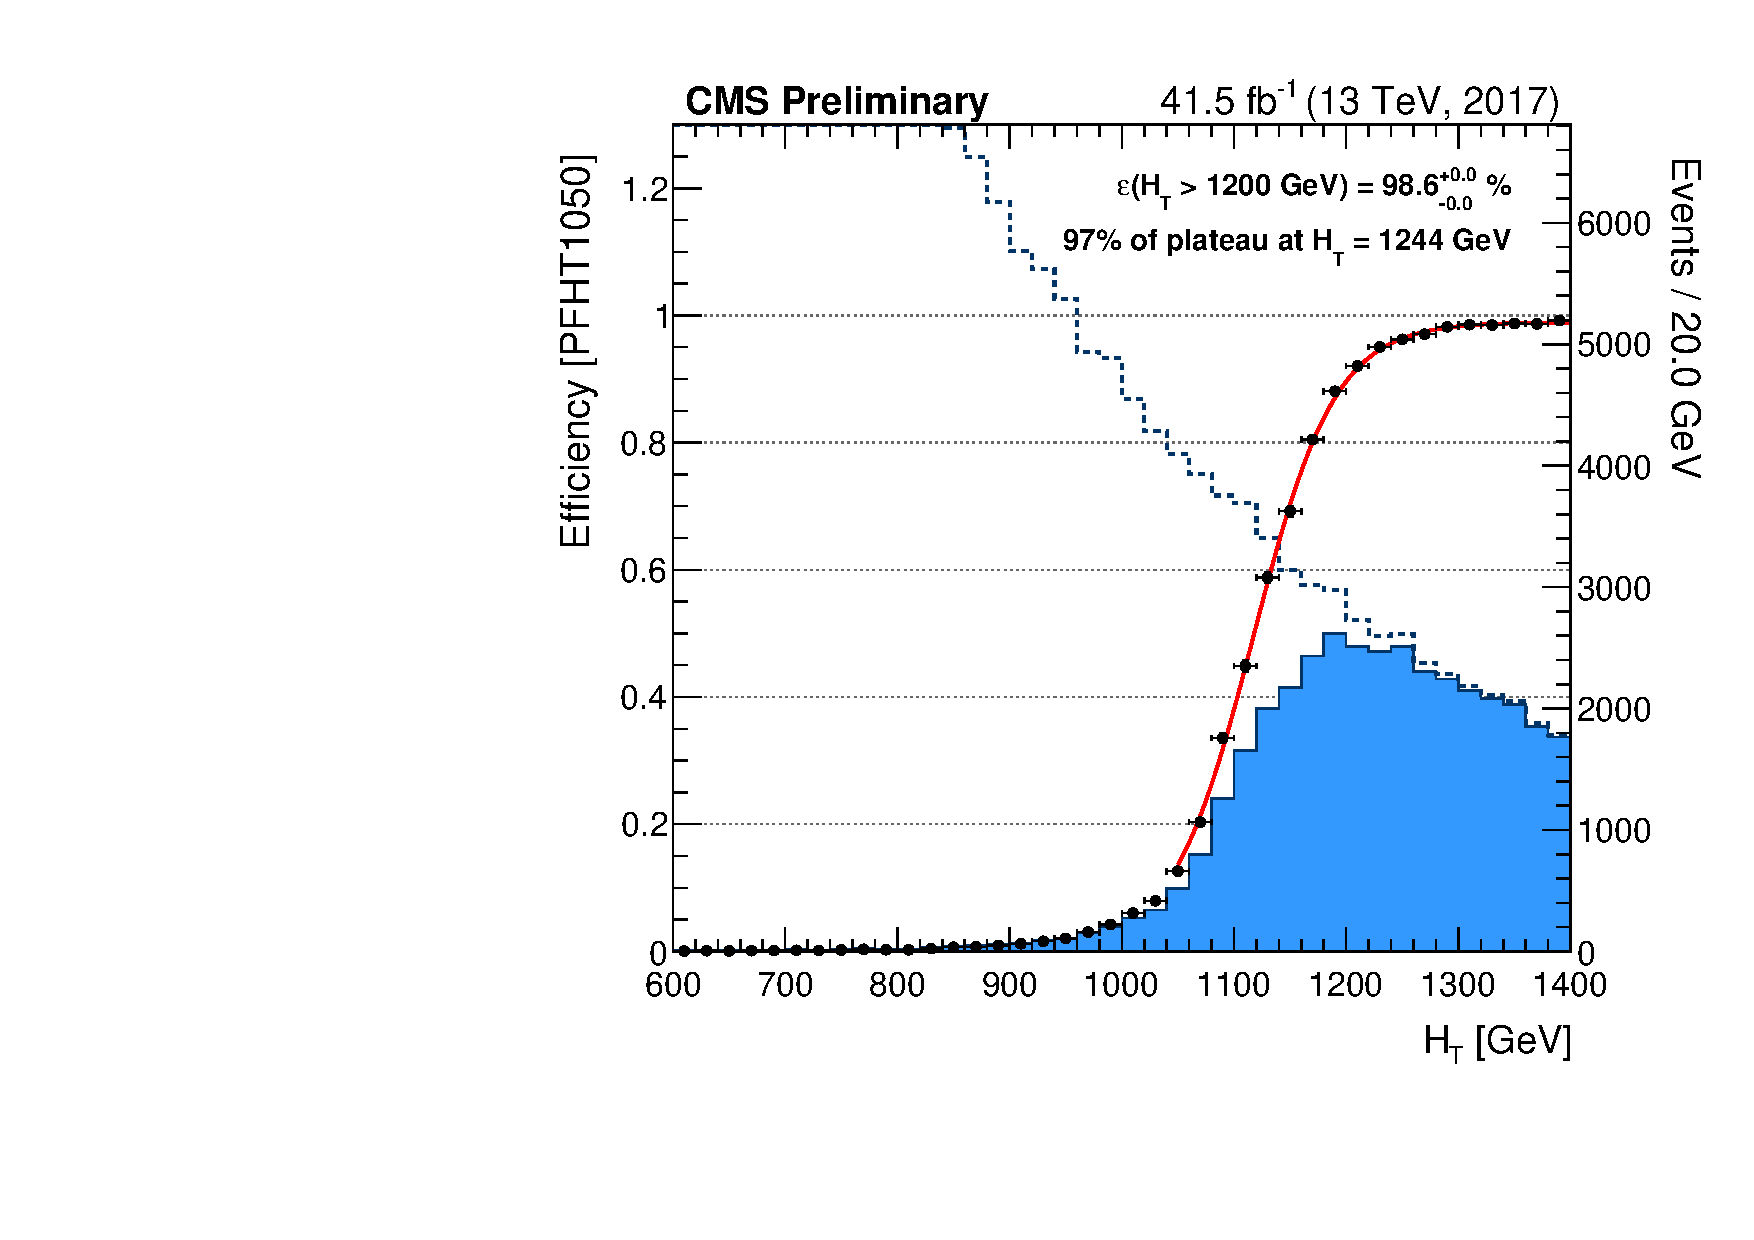
\includegraphics[width=0.49\textwidth]{figs/event_selection/pfht1050_2017_met.pdf}
    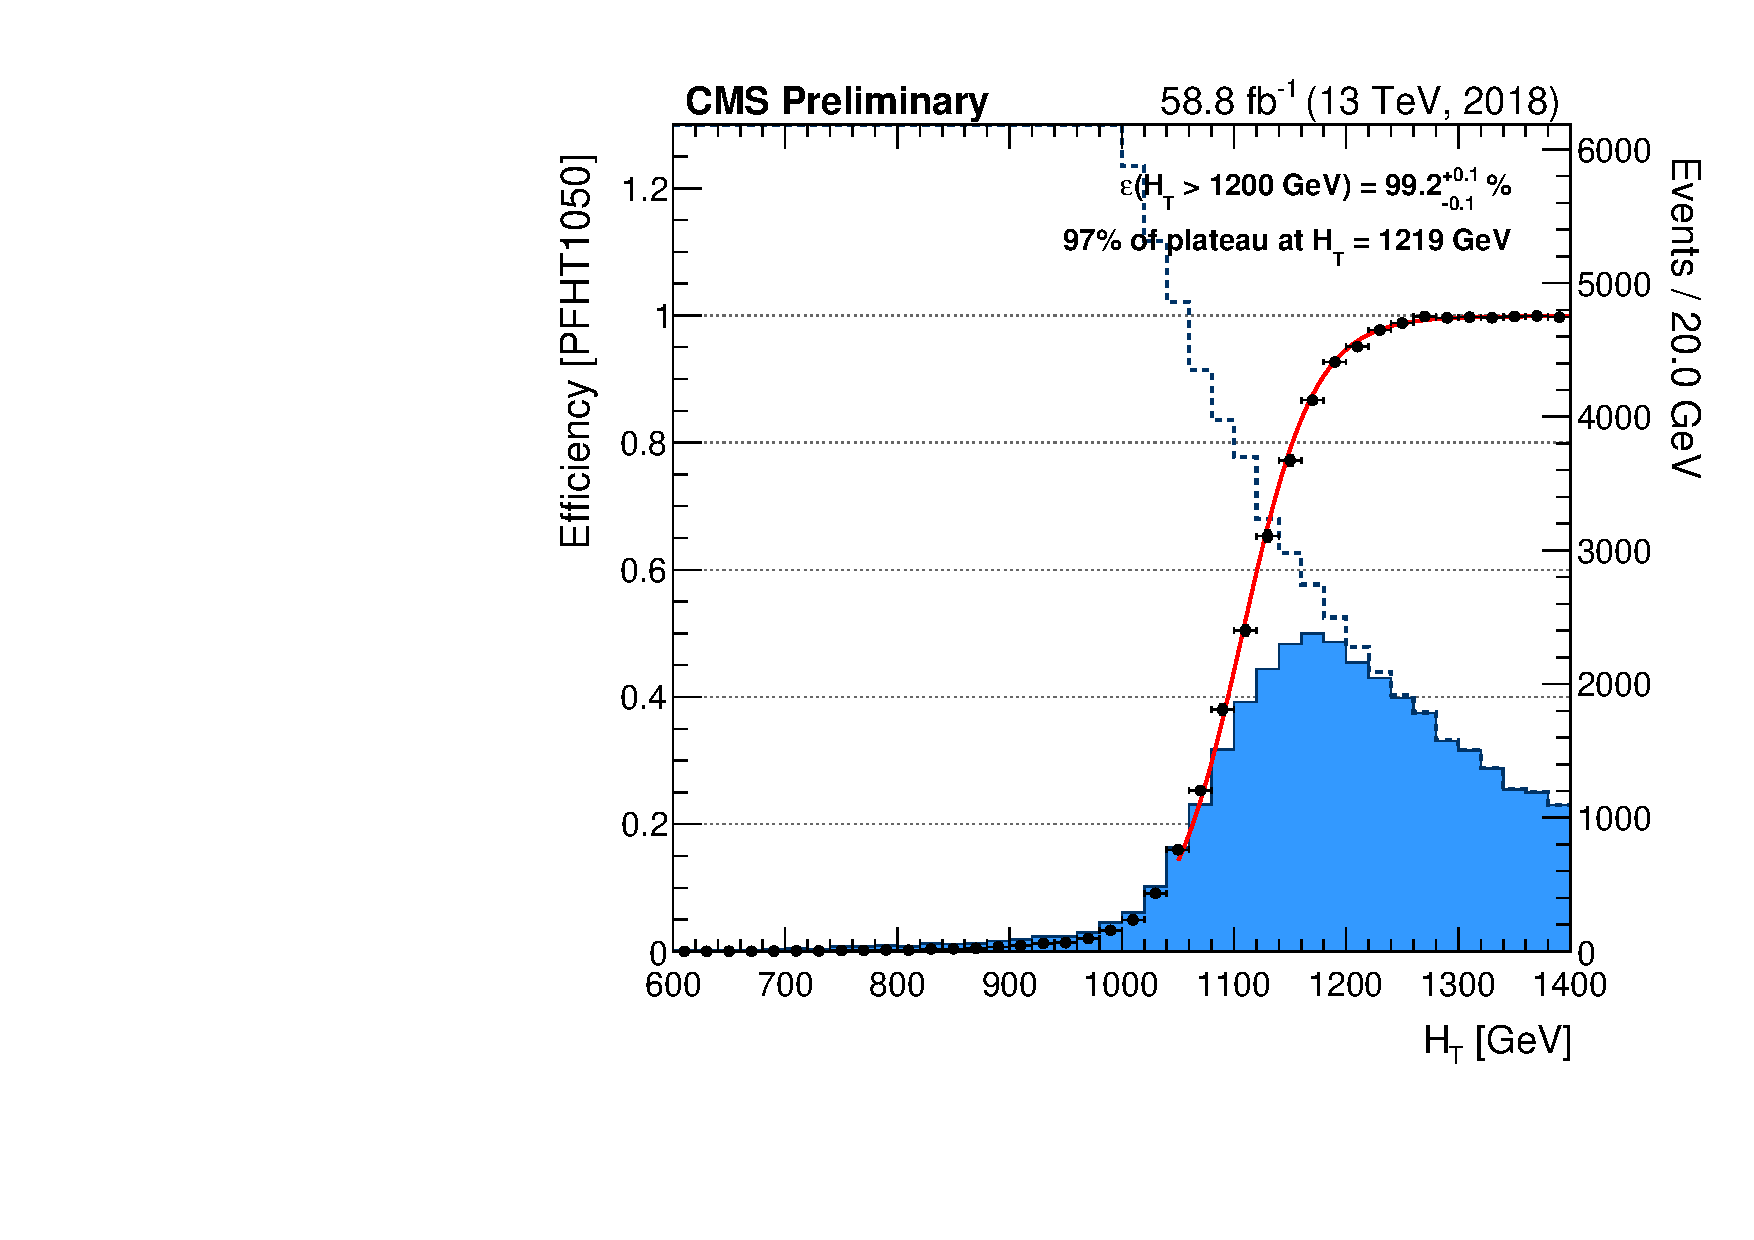
\includegraphics[width=0.49\textwidth]{figs/event_selection/pfht1050_2018_el.pdf}
    \caption{Trigger efficiency measurements for the pure-\Ht \texttt{HLT\_PFHT1050} trigger,
      (left) for 2017 data using a \ptmiss-based reference trigger, and (right) for 2018 data
      using an electron-based reference trigger. The dashed (solid) blue histograms
      are the denominator (numerator) event counts, and the red lines are logistic function fits to the
      efficiency curves.
            }
    \label{fig:trigmeas_HT}
  \end{center}
\end{figure}

The pure-\ptmiss trigger efficiencies are measured using the electron-based method described above.
The \Ht and \ptmiss leggs of the \Ht+\ptmiss triggers must be measured separately. The \Ht leg is measured
using a \ptmiss trigger reference, and the \ptmiss leg is measured using an electron trigger reference
(with the additional requirement of $\Ht>700\GeV$ to ensure that we are in the plateau of the \Ht leg).
Efficiencies of close to 100\% are observed in all cases. Example measurements of the \ptmiss and \Ht+\ptmiss
trigger efficienes are shown in Fig.~\ref{fig:trigmeas_HTMET}.

\begin{figure}[ht]
  \begin{center}
    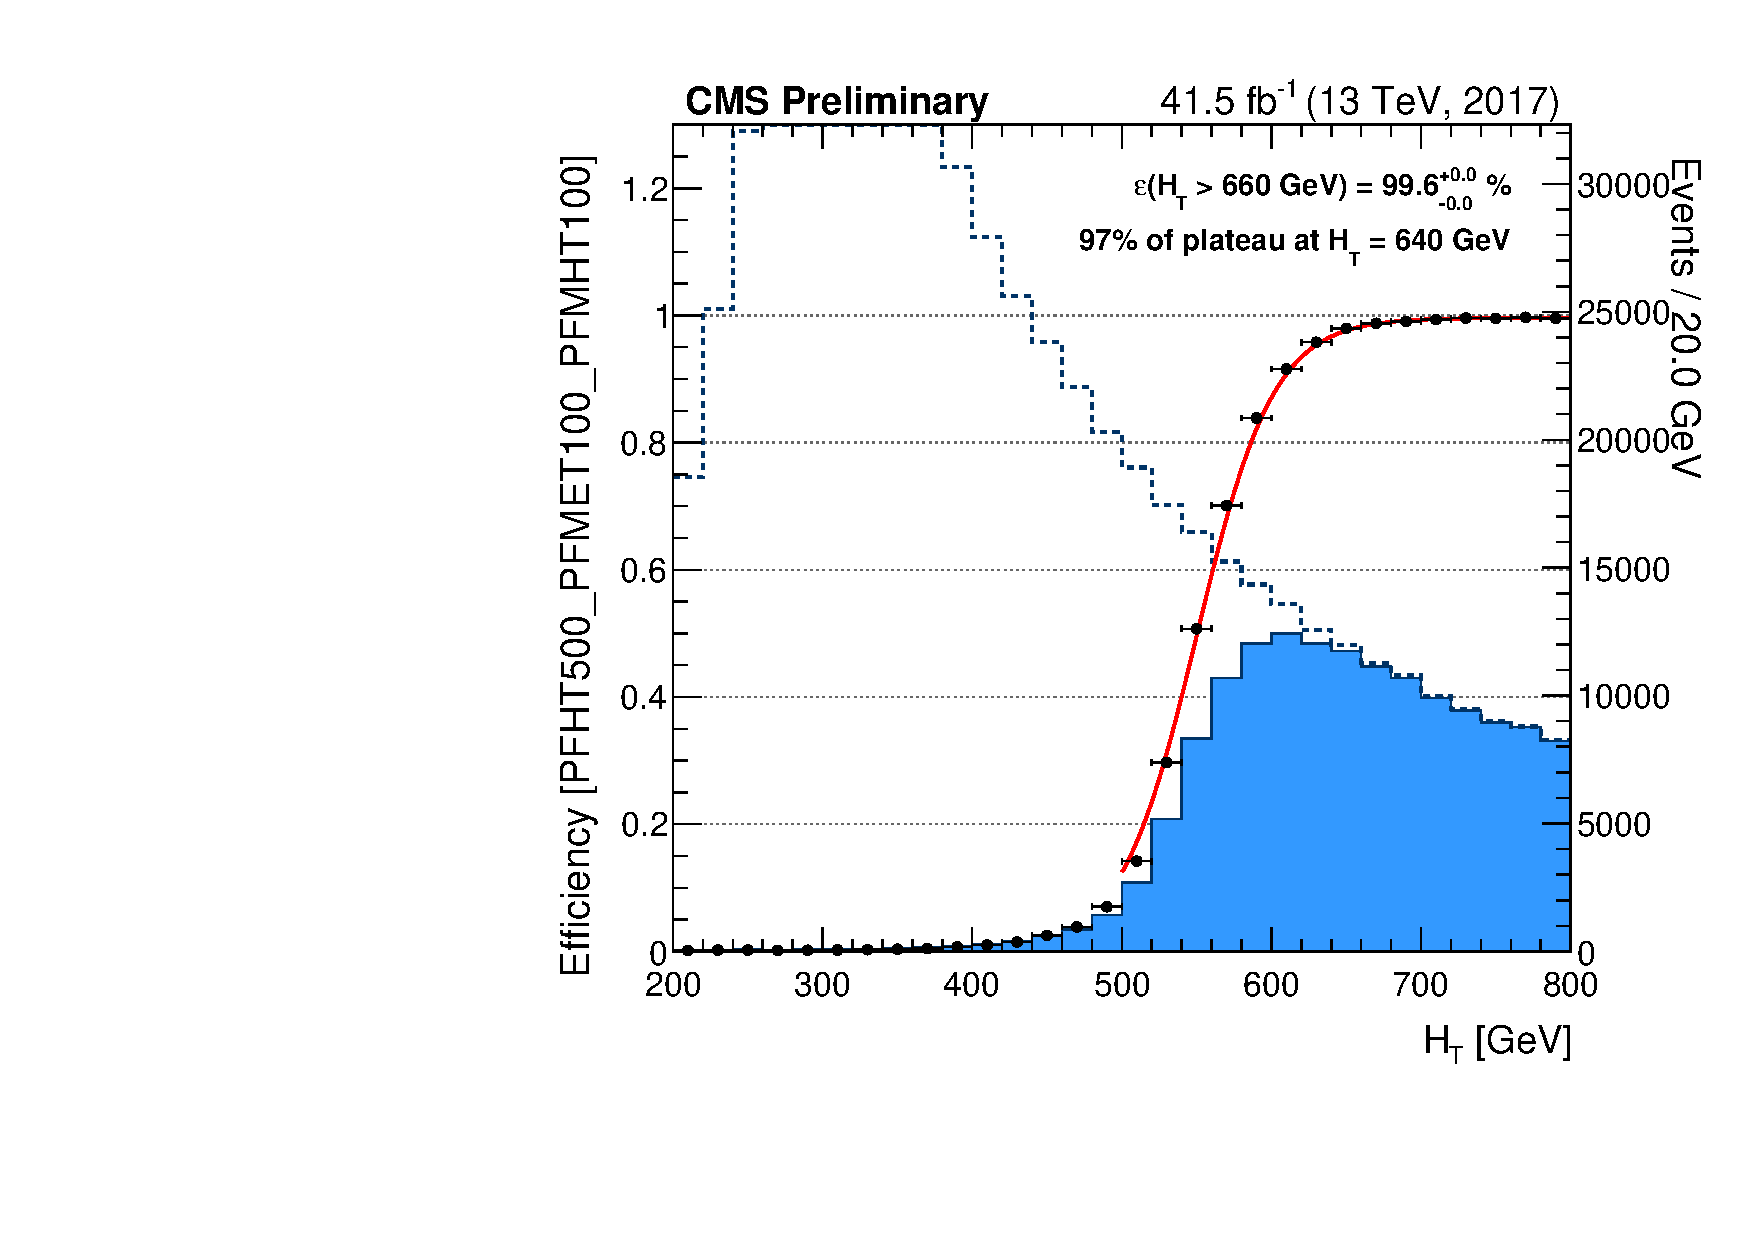
\includegraphics[width=0.49\textwidth]{figs/event_selection/pfht500met100_2017_htleg_met.pdf}
    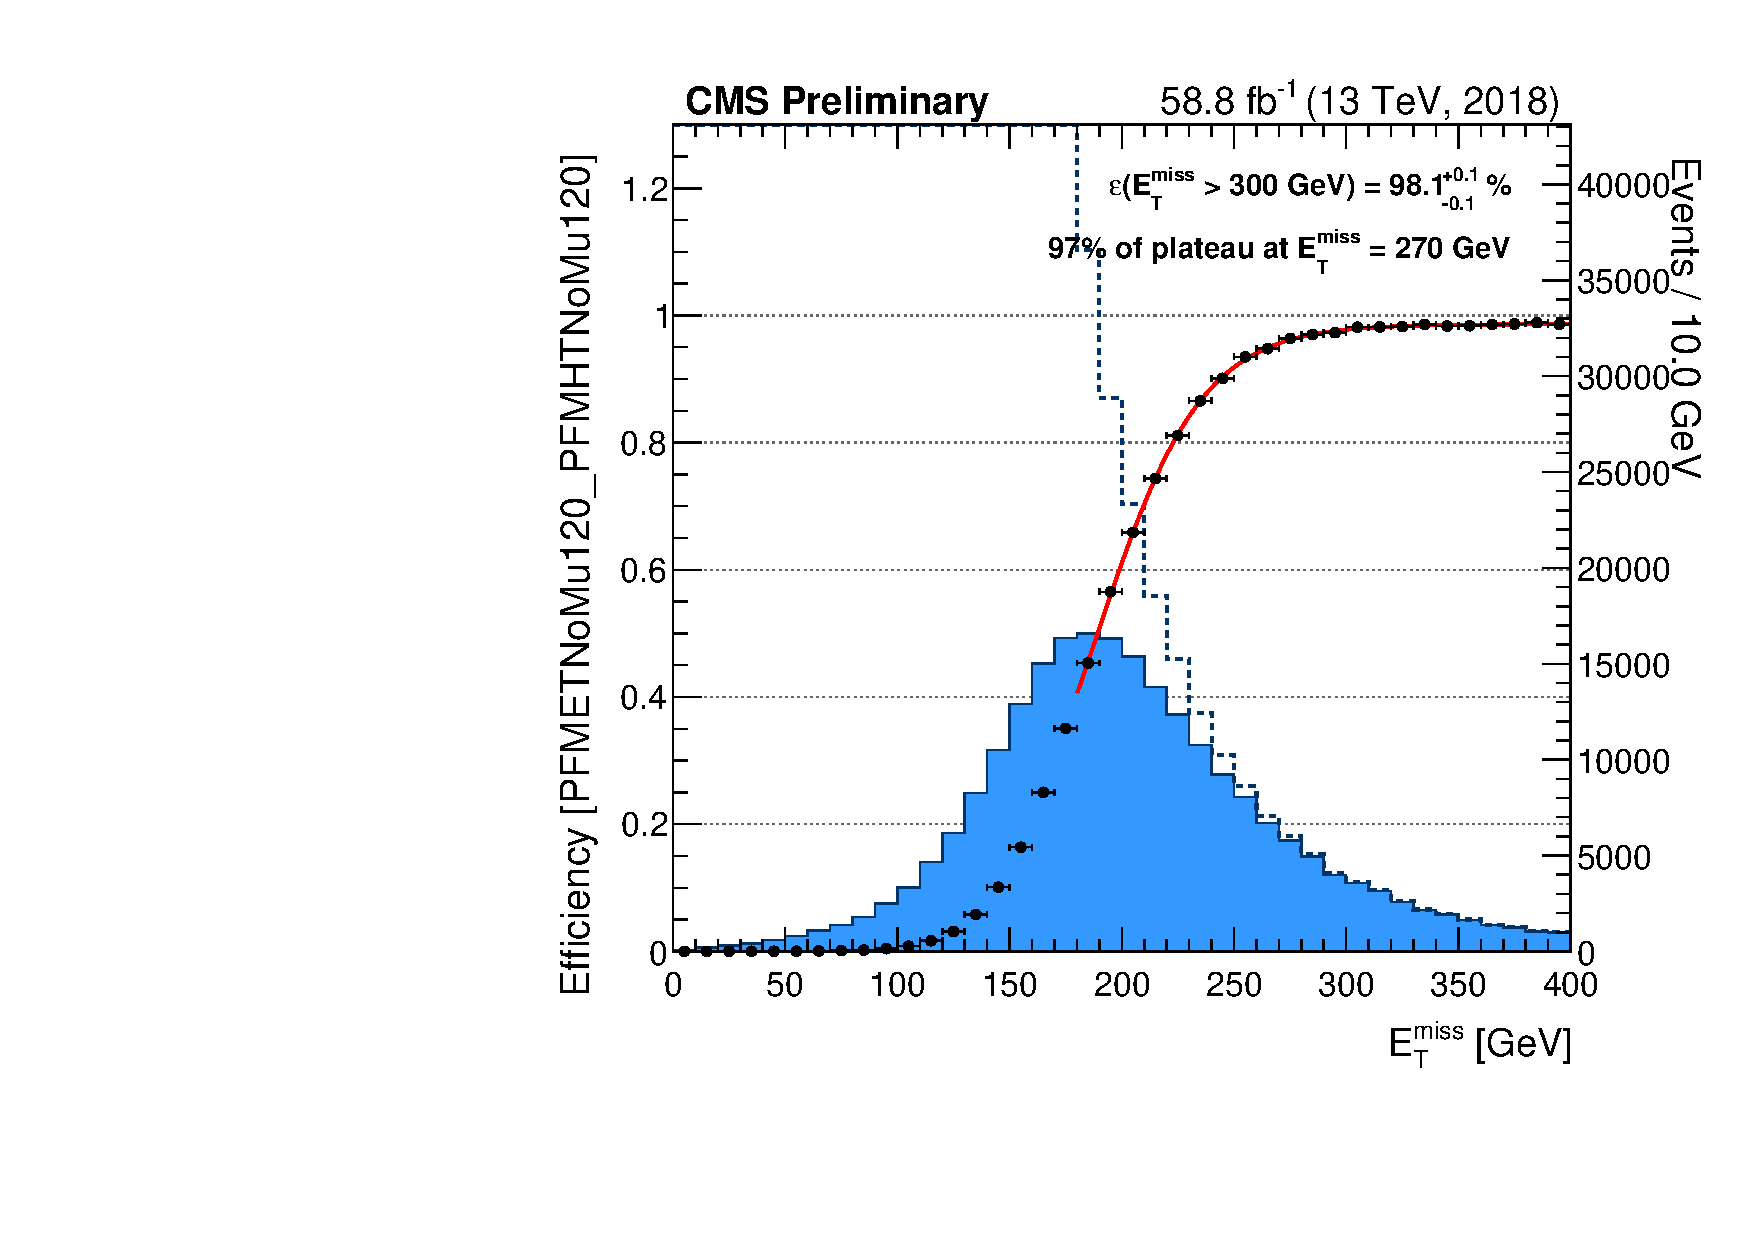
\includegraphics[width=0.49\textwidth]{figs/event_selection/pfmet120nomu_2018_el.pdf}
    \caption{Trigger efficiency measurements (left) for the \Ht-leg of the \texttt{HLT\_PFHT500\_PFMET100}
      trigger in 2017 data, measured with a \ptmiss-based reference trigger, 
      and (right) for the pure-\ptmiss \texttt{HLT\_PFMETNoMu120\_PFMHTNoMu120} trigger
      in 2018 data, measured using an electron-based reference trigger. The dashed (solid) blue histograms
      are the denominator (numerator) event counts, and the red lines are logistic function fits to the
      efficiency curves.
            }
    \label{fig:trigmeas_HTMET}
  \end{center}
\end{figure}

\subsection{Control region triggers}
\label{sec:crtrigs}

Control region definitions are given in Sec.~\ref{sec:crdefs}. Here we only summarize the triggers used,
and it is sufficient to know that there are both single lepton and dilepton control regions used for
predicting the electroweak backgrounds, and an inclusive low-\Ht data sample used in the estimate
of the QCD multijet background.

The single lepton control region is triggered with the same triggers as the signal region, since
the cuts on the relevant kinematic variables are the same (the only difference is the requirement of
exactly one lepton, instead of zero).

This is not true for the dilepton control region, since as we will see the leptons are removed from
the \Ht and added to the \vMet vector before cutting on these variables. So the standard \Ht and
\ptmiss triggers will not work, and special dilepton triggers are used instead.

The dimuon selection is triggered with a combination of isolated and non-isolated
dimuon triggers and non-isolated single-muon triggers (non-isolated and single-muon
paths are to recover inefficiencies at high muon \pt).

Similarly, the dielectron selection is triggered with a combination of isolated and non-isolated
dielectron triggers as well as a single-photon trigger.

Finally, there is an different-flavor (i.e. $e\mu$) control regoin used for estimating \ttbar contamination
in the same-flavor region, that is triggered with a combination of isolated and non-isolated
$e\mu$ triggers, non-isolated single-muon triggers, and a single-photon trigger.

Efficiencies of these dilepton can be measured using pure-\Ht triggers as a reference (both non-prescaled
and lower threshold prescaled triggers).
Plots of measured trigger efficiency as a function of leading and subleading lepton \pt in the relevant
section of phase space are shown in Fig.~\ref{fig:trigmeas_dilep}, for 2017 data. Measurements for 2016 
and 2018 are similar. Inefficiencies up to $\sim10$\% are present; these are accounted for by
applying them as weights to MC on a year-by-year basis as a function of leading and subleading \pt.

\begin{figure}[t]
  \begin{center}
    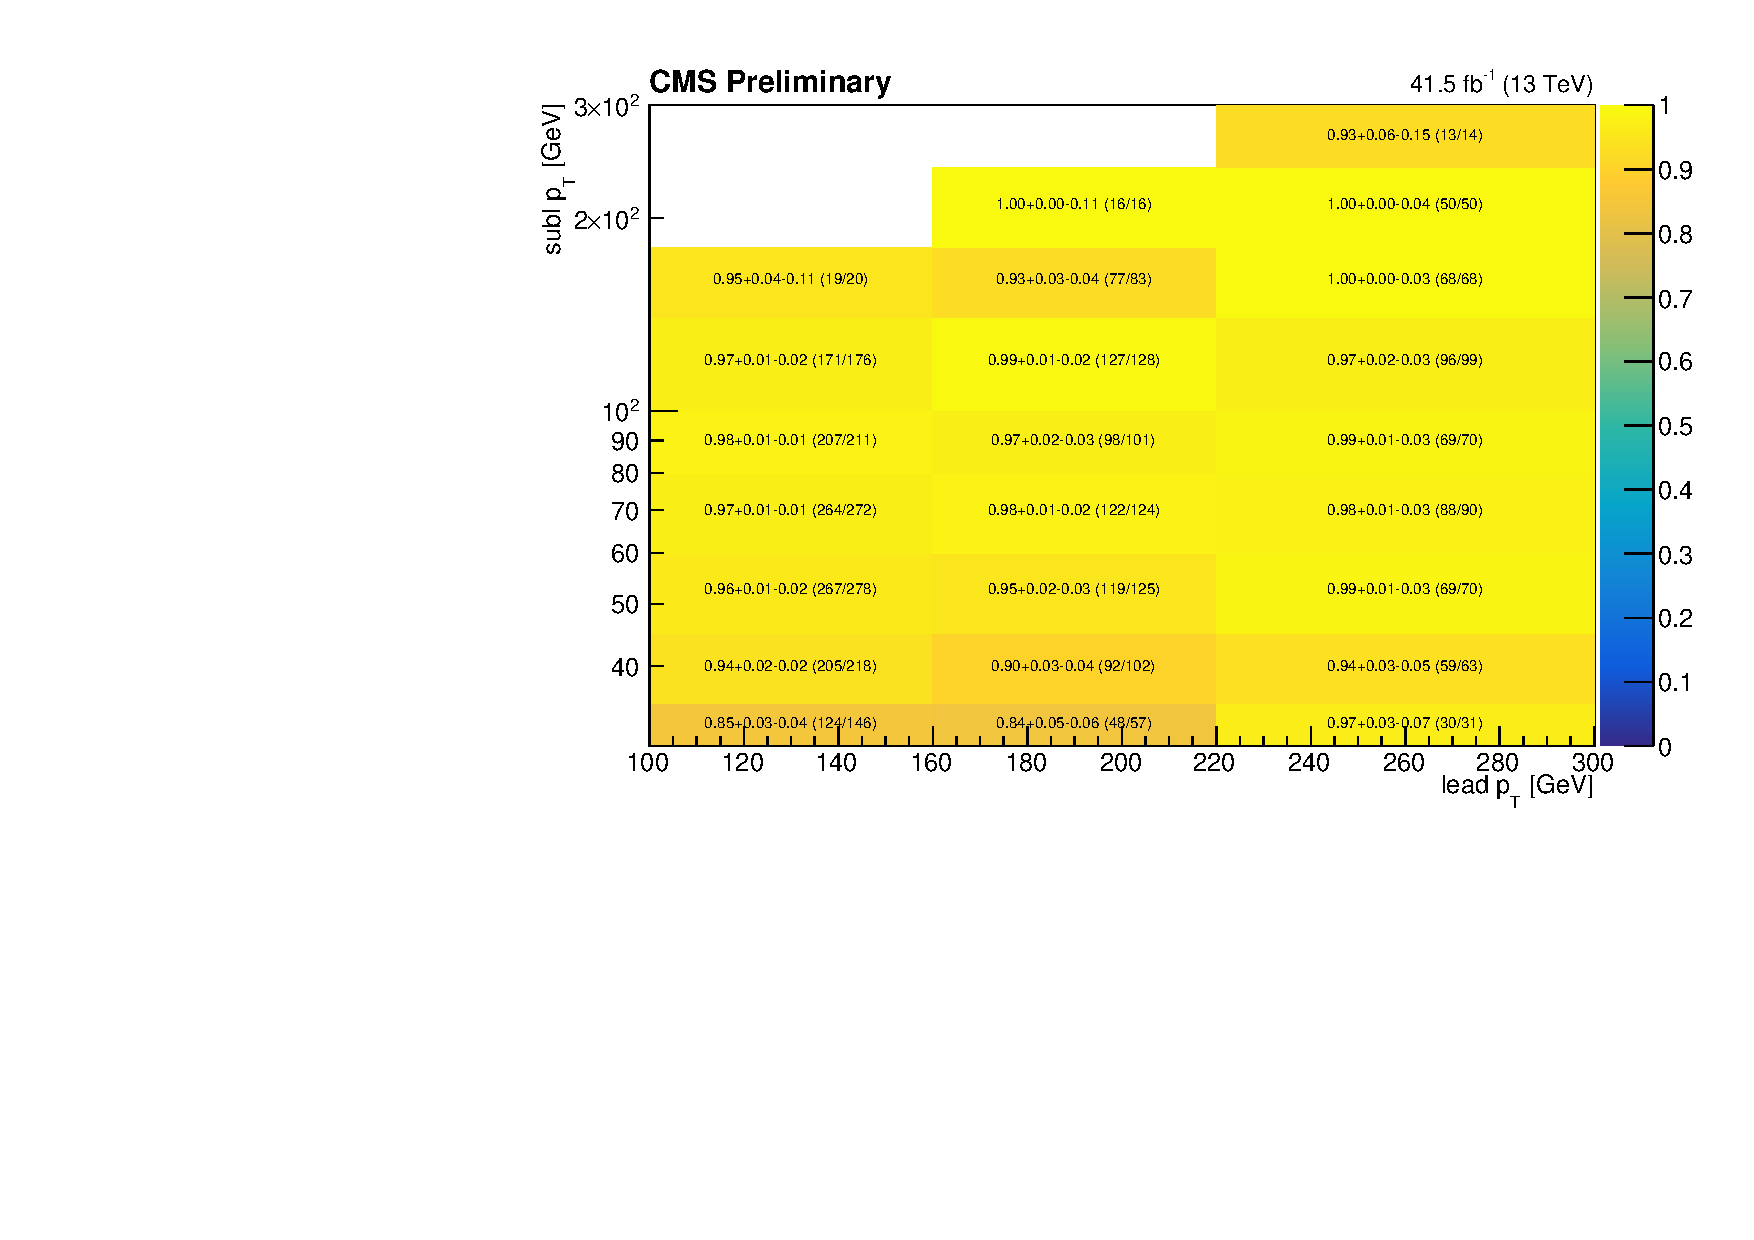
\includegraphics[width=0.49\textwidth]{figs/event_selection/trigeff_dilep_mm_2d_ht_2017fullYear.pdf}
    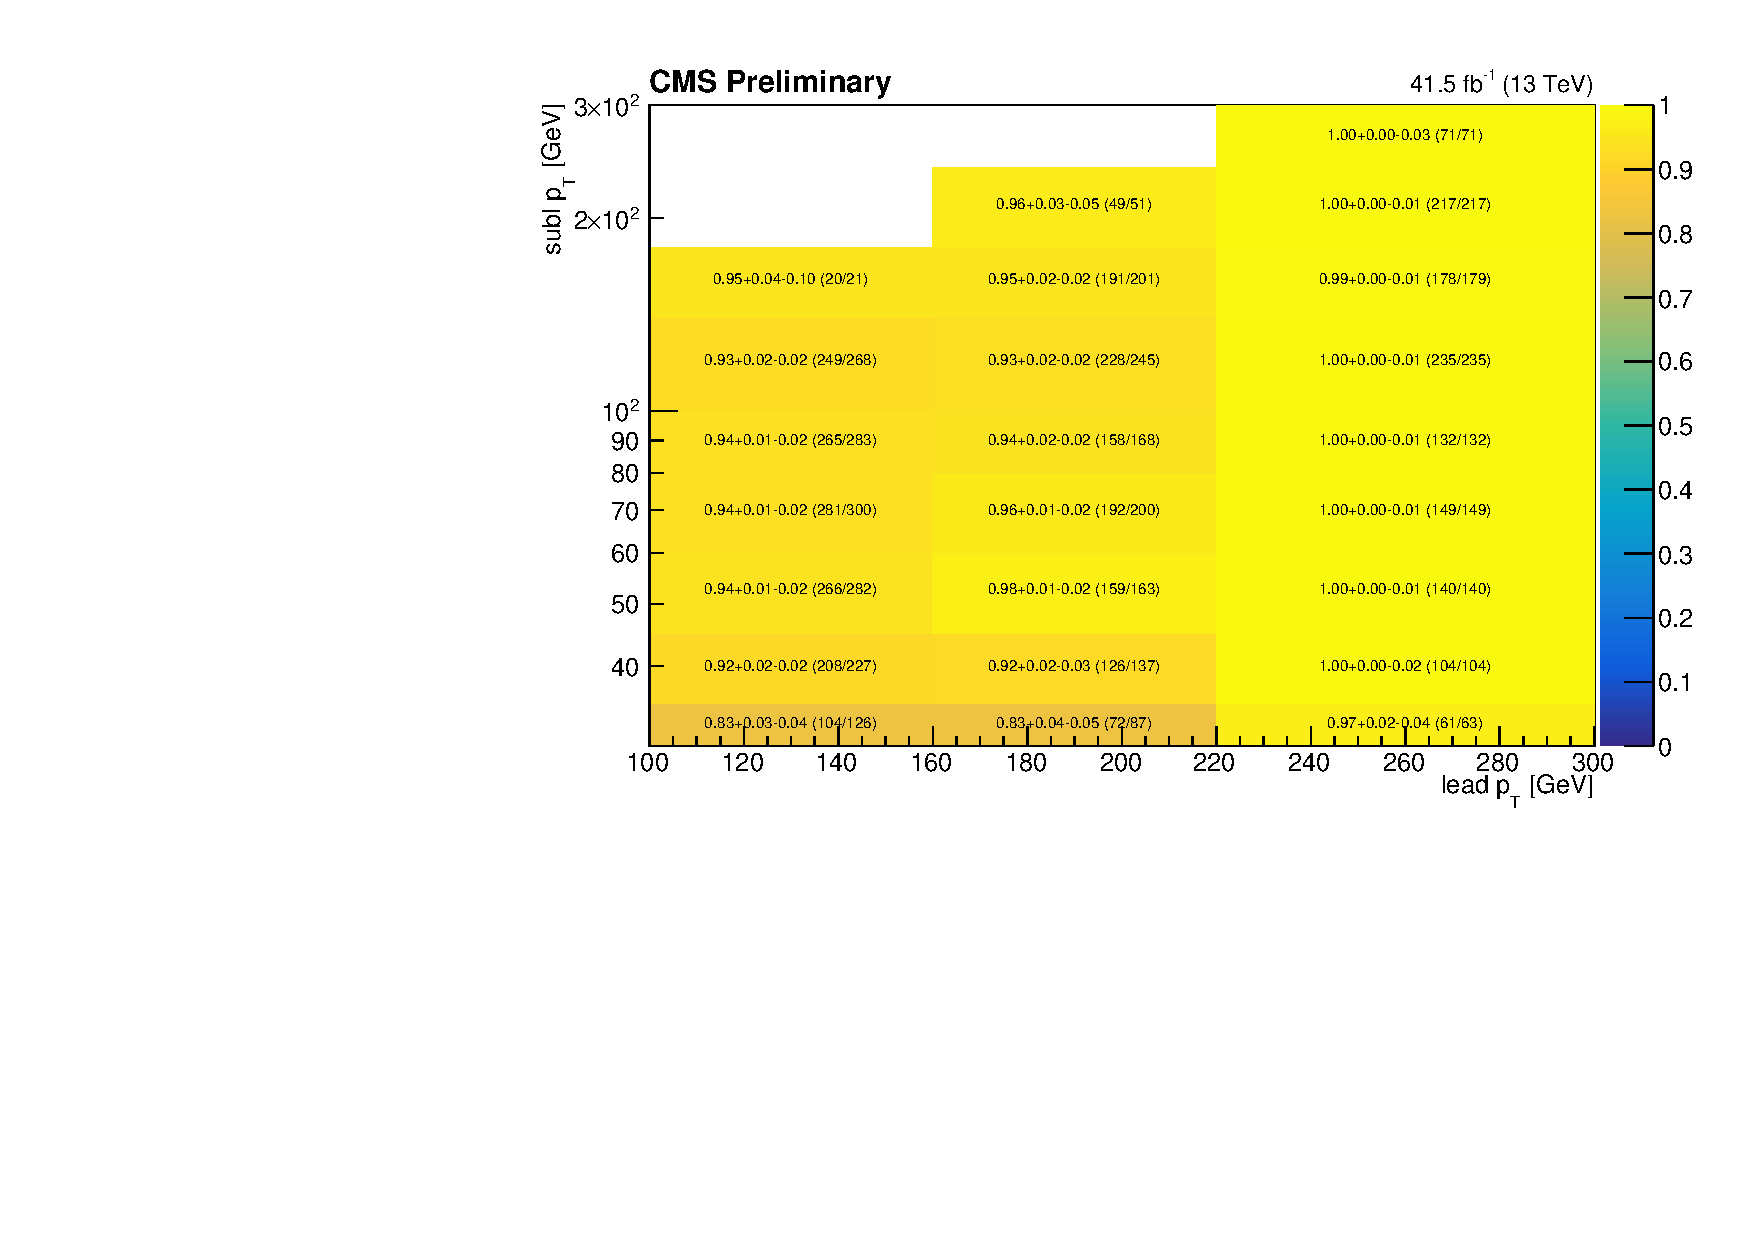
\includegraphics[width=0.49\textwidth]{figs/event_selection/trigeff_dilep_ee_2d_ht_2017fullYear.pdf} \\
    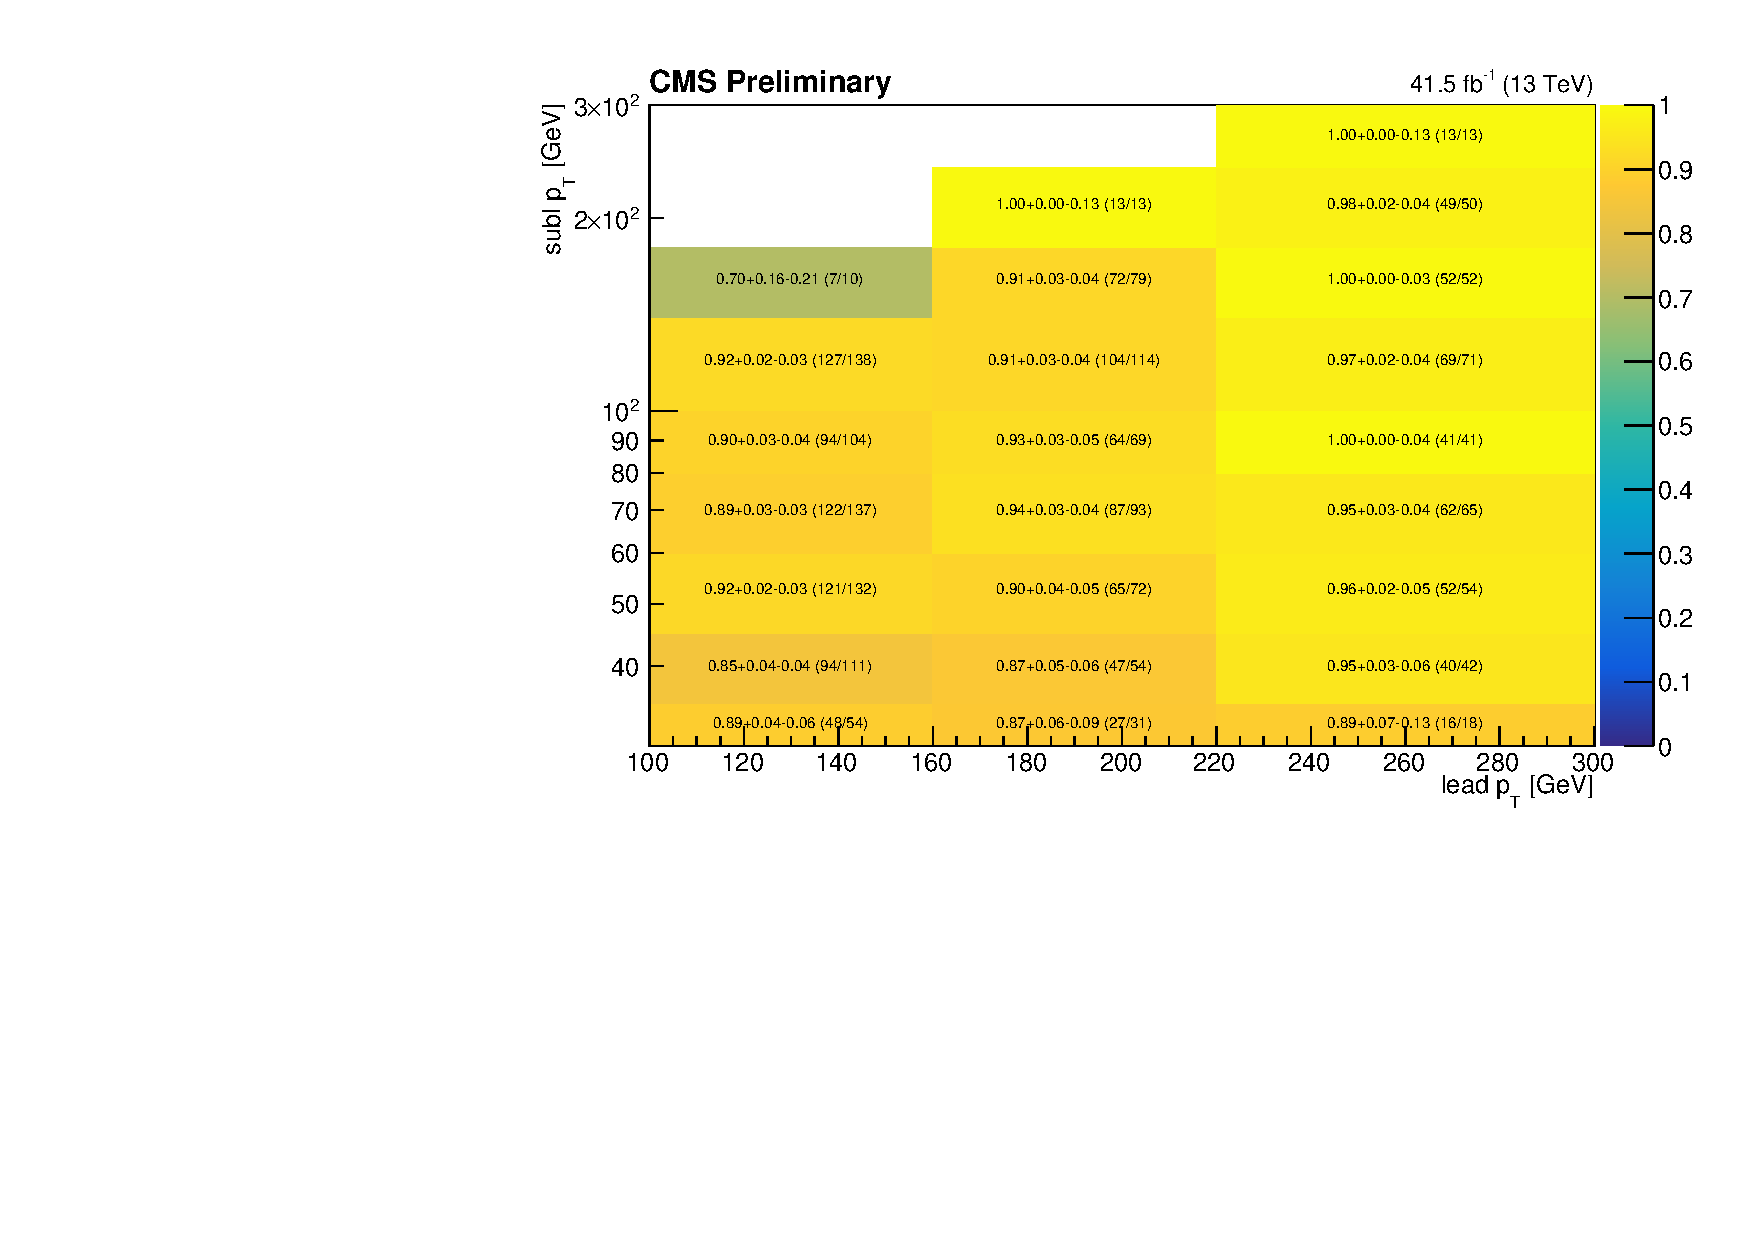
\includegraphics[width=0.49\textwidth]{figs/event_selection/trigeff_dilep_em_2d_ht_2017fullYear.pdf}
    \caption{Measured dilepton trigger efficiences as a function of leading and subleading lepton \pt
      in 2017 data, for (top left) dimuon, (top right) dielectron,
      and (bottom) $e\mu$ selections. Triggers used are a logical OR of the various triggers described
      in Sec.~\ref{sec:crtrigs}. Measurements in 2016 and 2018 are similar.
            }
    \label{fig:trigmeas_dilep}
  \end{center}
\end{figure}

Though not technically a control region, an inclusive selection of low-\Ht events is used in the Rebalance and
Smear method for computing QCD multijet background, described in Chapter~\ref{chap:qcd}. This selection
makes use of low-threshold pure-\Ht triggers, that are necessarily prescaled due to their very
high rates. Though event-by-event prescale values are stored in the data (the exact prescale rate
depends on the instantaneous luminosity and the exact trigger menu being used, so vary with time),
yearly ``effective prescales'' are measured as a constistency check. This is done by measuring the
ratio of rates of different triggers as a function of \Ht, and fitting the ratio
in the plateau. Comparing to the high threshold unprescaled trigger, the effective prescales of
all others can be determined.

A plot measuring the effective prescales in 2017 data is shown in Fig.~\ref{fig:pureht_prescales} (left).
On the right is the observed \Ht spectrum using these prescale values, which is smooth as
is expected if the correct prescales are measured.

\begin{figure}[t]
  \begin{center}
    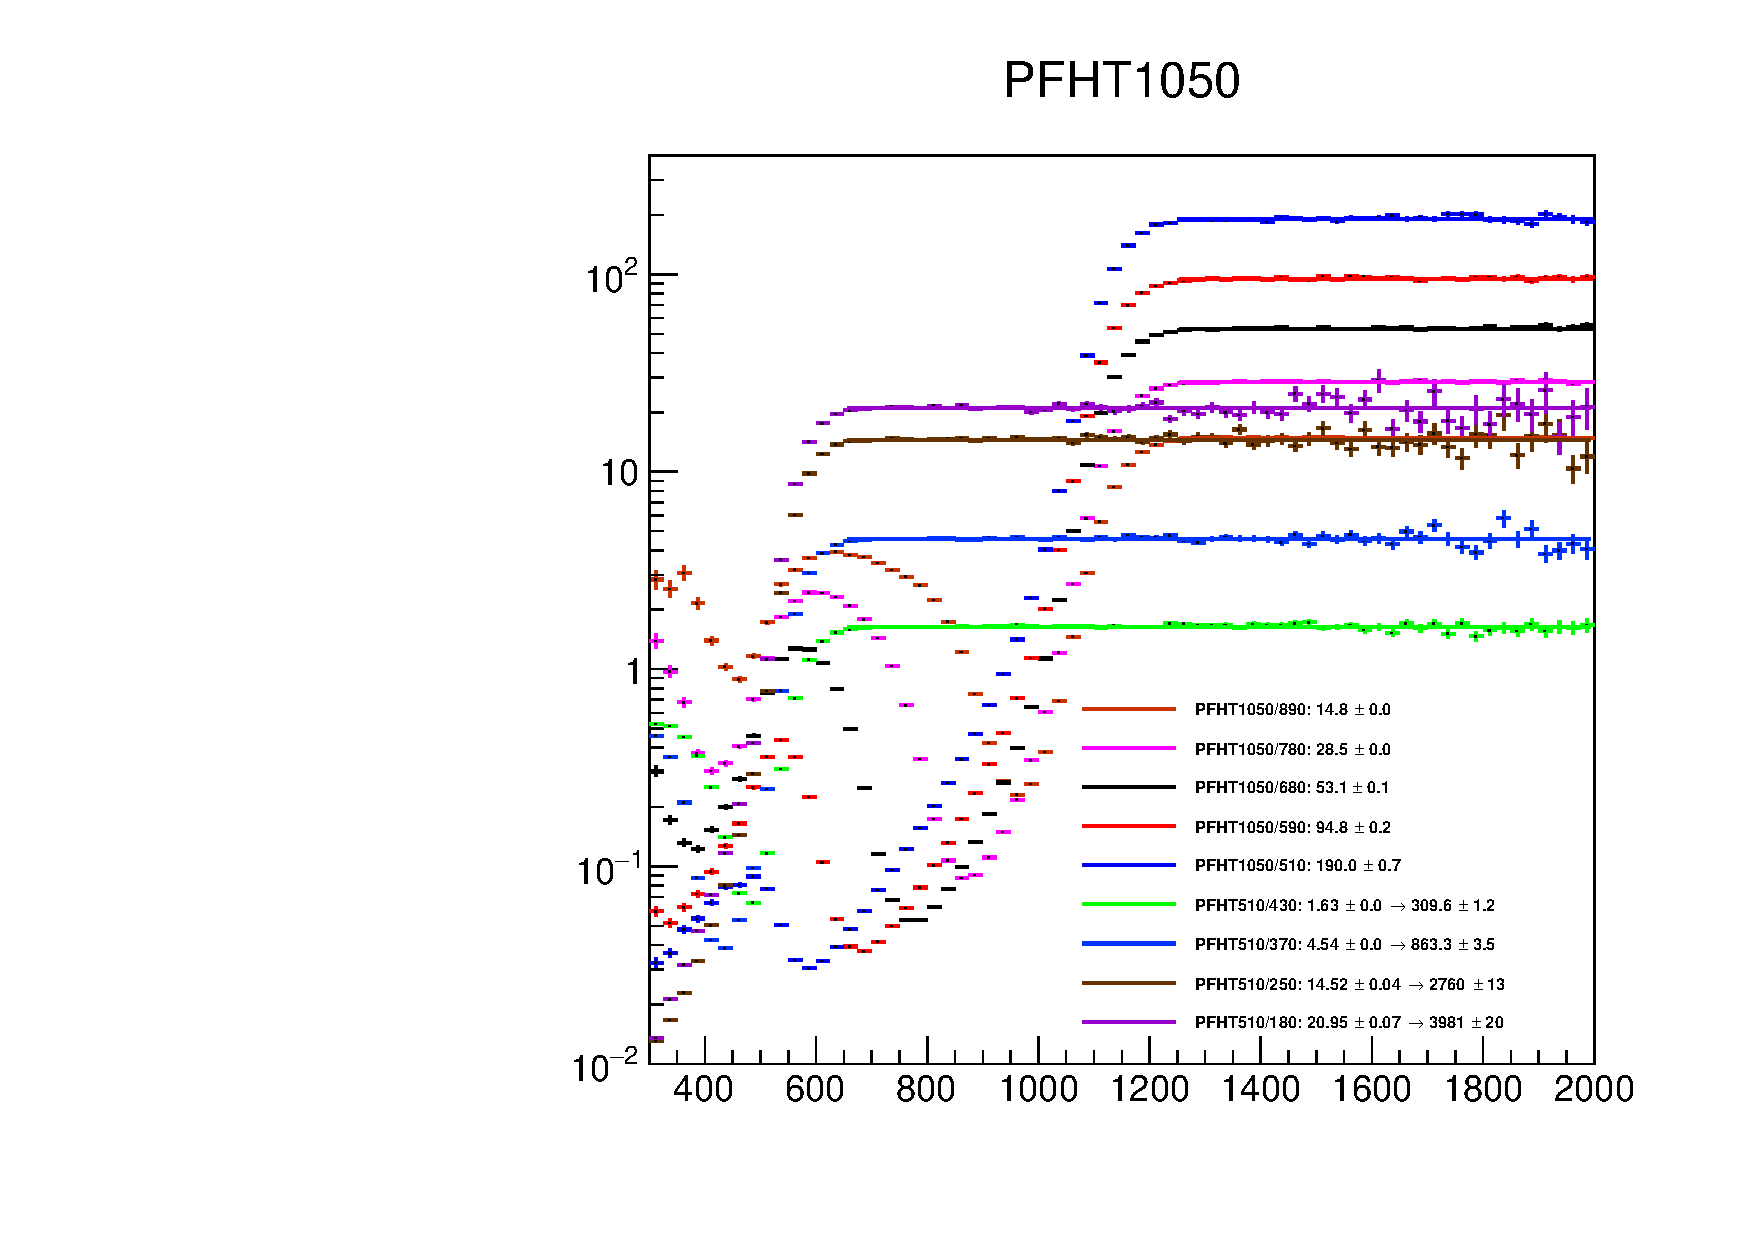
\includegraphics[width=0.45\textwidth]{figs/event_selection/prescales_2017.pdf}
    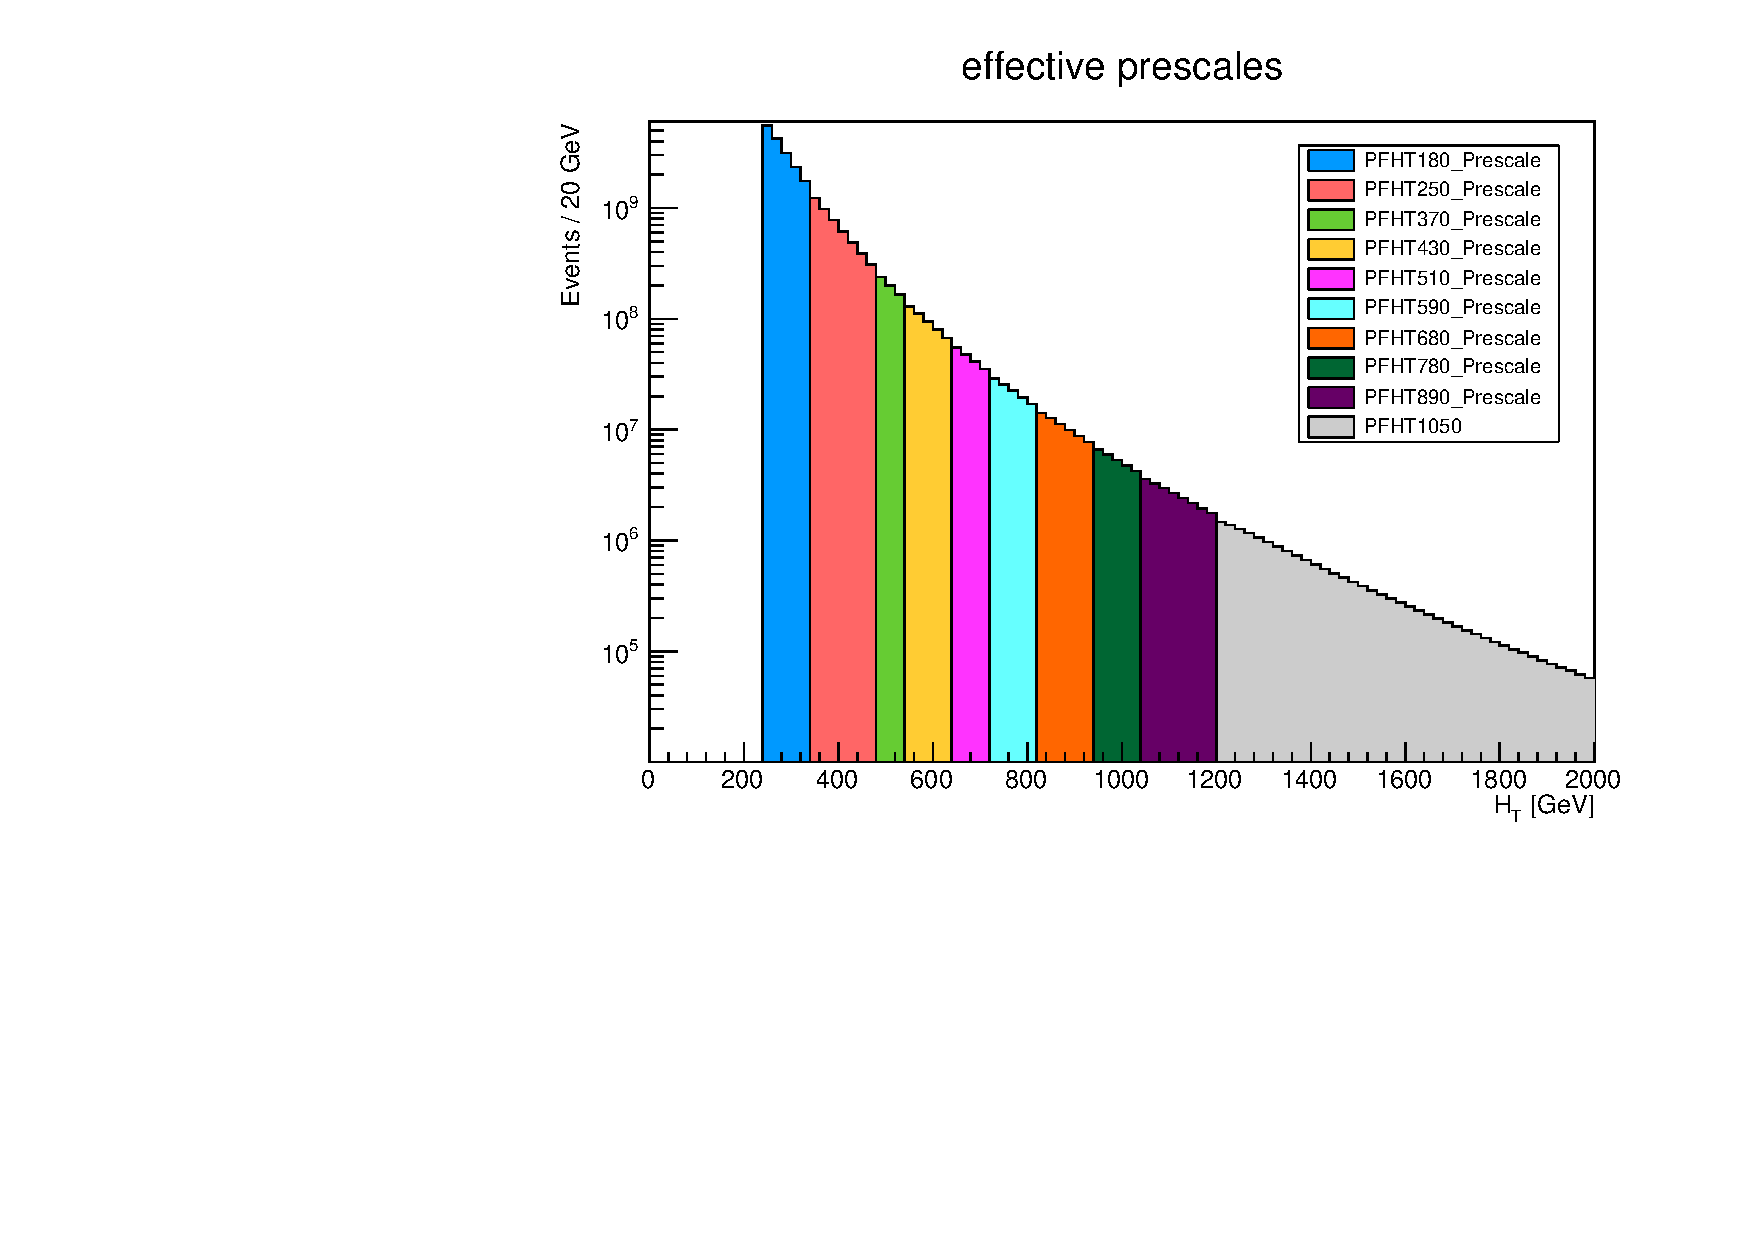
\includegraphics[width=0.54\textwidth]{figs/event_selection/htSpect2017_meth1.pdf} \\
    \caption{(left) A plot of the ratio of rates of various pure-\Ht triggers in
      2017 data. The value at the plateau gives the relative prescale between two triggers,
      and comparing to the unprescaled \texttt{HLT\_PFHT1050} gives the absolute prescale.
      (right) The observed \Ht spectrum using these prescales, which is smooth as is expected 
      if the correct values are measured.
            }
    \label{fig:pureht_prescales}
  \end{center}
\end{figure}

\section{Baseline selection}
\label{sec:baselinesel}

Using the object and variable definitions detailed in Sec.~\ref{sec:objvardefs}, the
baseline selection used for all analysis signal regions is as follows:
\begin{itemize}\setlength\itemsep{-1mm}
\item at least one good vertex, as defined in Sec.~\ref{sec:vertices}
\item pass all \ptmiss filters, as defined in Sec.~\ref{sec:metfilters}
\item pass the logical OR of all signal region triggers listed in Sec.~\ref{sec:srtrigs}
\item $\Ht>1200\GeV$ and $\ptmiss>30\GeV$, or $\Ht>250\GeV$ and $\ptmiss>250\GeV$. These cuts are
based on the available trigger thresholds, and illustrated in Fig.~\ref{fig:trig_diagram}.
\item $\dphimet>0.3$. This protects against large \ptmiss from jet mis-measurement in multijet events,
and rejects a large fraction of QCD background.
\item $|\vMht-\vMet|/\ptmiss<0.5$. This requires that \vMht be similar to \vMet, and in doing so
protects agains bias in the shape of \mttwo. \ptmiss is sensitive to reconstructed objects with
$\pt<30\GeV$ or $|\eta|>2.4$, where as these are not used in \vMht or in the construction of
pseudojets for \mttwo, so a large contribution from these objects to the missing transverse energy
can bias the \mttwo distribution.
\item lepton veto: to reduce the background from events with a $W$ boson decay, we reject events if they contain
\vspace{-\topsep}
\begin{itemize}\setlength\itemsep{-1mm}
\item a reconstructed electron or muon as defined in Secs.~\ref{sec:electrons} and \ref{sec:muons}
\item a particle-flow electron, muon, or hadron candidate as defined in Sec.~\ref{sec:isotracks},
with the additional requirement of $M_\mrm{T}(\mrm{cand},\vMet)<100\GeV$ (to avoid vetoing
signal events, which contain \ptmiss not from the leptonic $W$ decay and hence have high $M_\mrm{T}$).
\end{itemize}
\item $\mttwo>200\GeV$ (only for events with at least 2 jets). This provides a large rejection of QCD
multijet events that have large \ptmiss from mis-measured jets, as discussed in Sec.~\ref{sec:mt2_variable}.
The threshold is raised to $\mttwo>400\GeV$ for events with $\Ht>1500\GeV$, in order to ensure that
QCD multijet events remain a subdominant background.
\end{itemize}

\section{Signal region definitions}
\label{sec:srdefs}

After the baseline selection defined in Sec.~\ref{sec:baselinesel}, signal regions are further categorized
into different bins of \Ht, \Nj, \Nb, and \mttwo.

First, we categorize $\Nj\geq2$ (multijet) events by \Ht, \Nj, and \Nb. Each $(\Ht,\Nj,\Nb)$ bin is referred to as a
\emph{topological region}.
\begin{itemize}\setlength\itemsep{-1mm}
\item Five \Ht regions: $[250,450],[450,575],[575,1200],[1200,1500],[1500,\infty]$\GeV.
These bins are referred to here and throughout this dissertation as Very Low, Low, Medium,
High, and Extreme \Ht, respectively.
\item For the first three \Ht regions, we use 11 bins in \Nj and \Nb:
\vspace{-\topsep}
\begin{itemize}\setlength\itemsep{-1mm}
\item 2--3 jets; 0, 1, 2 b tags
\item 4--6 jets; 0, 1, 2 b tags
\item 2--6 jets; $\geq$3 b tags
\item $\geq$7 jets; 0, 1, 2, $\geq$3 b tags
\end{itemize}
\item For the highest two \Ht regions, we further subdivide the $\Nj\geq7$ regions
for a total of 17 bins in \Nj and \Nb:
\vspace{-\topsep}
\begin{itemize}\setlength\itemsep{-1mm}
\item 2--3 jets; 0, 1, 2 b tags
\item 4--6 jets; 0, 1, 2 b tags
\item 2--6 jets; $\geq$3 b tags
\item 7--9 jets; 0, 1, 2, 3, $\geq$4 b tags
\item $\geq$10 jets; 0, 1, 2, 3, $\geq$4 b tags
\end{itemize}
\end{itemize}

The division into topological regions for the High \Ht region is shown in Fig.\ref{fig:piechart_H}, along
with background composition in each region. We see that QCD multijet background becomes more important with
increasing \Nj, and top background becomes more dominant with increasing \Nb.

\begin{figure}[t]
  \begin{center}
    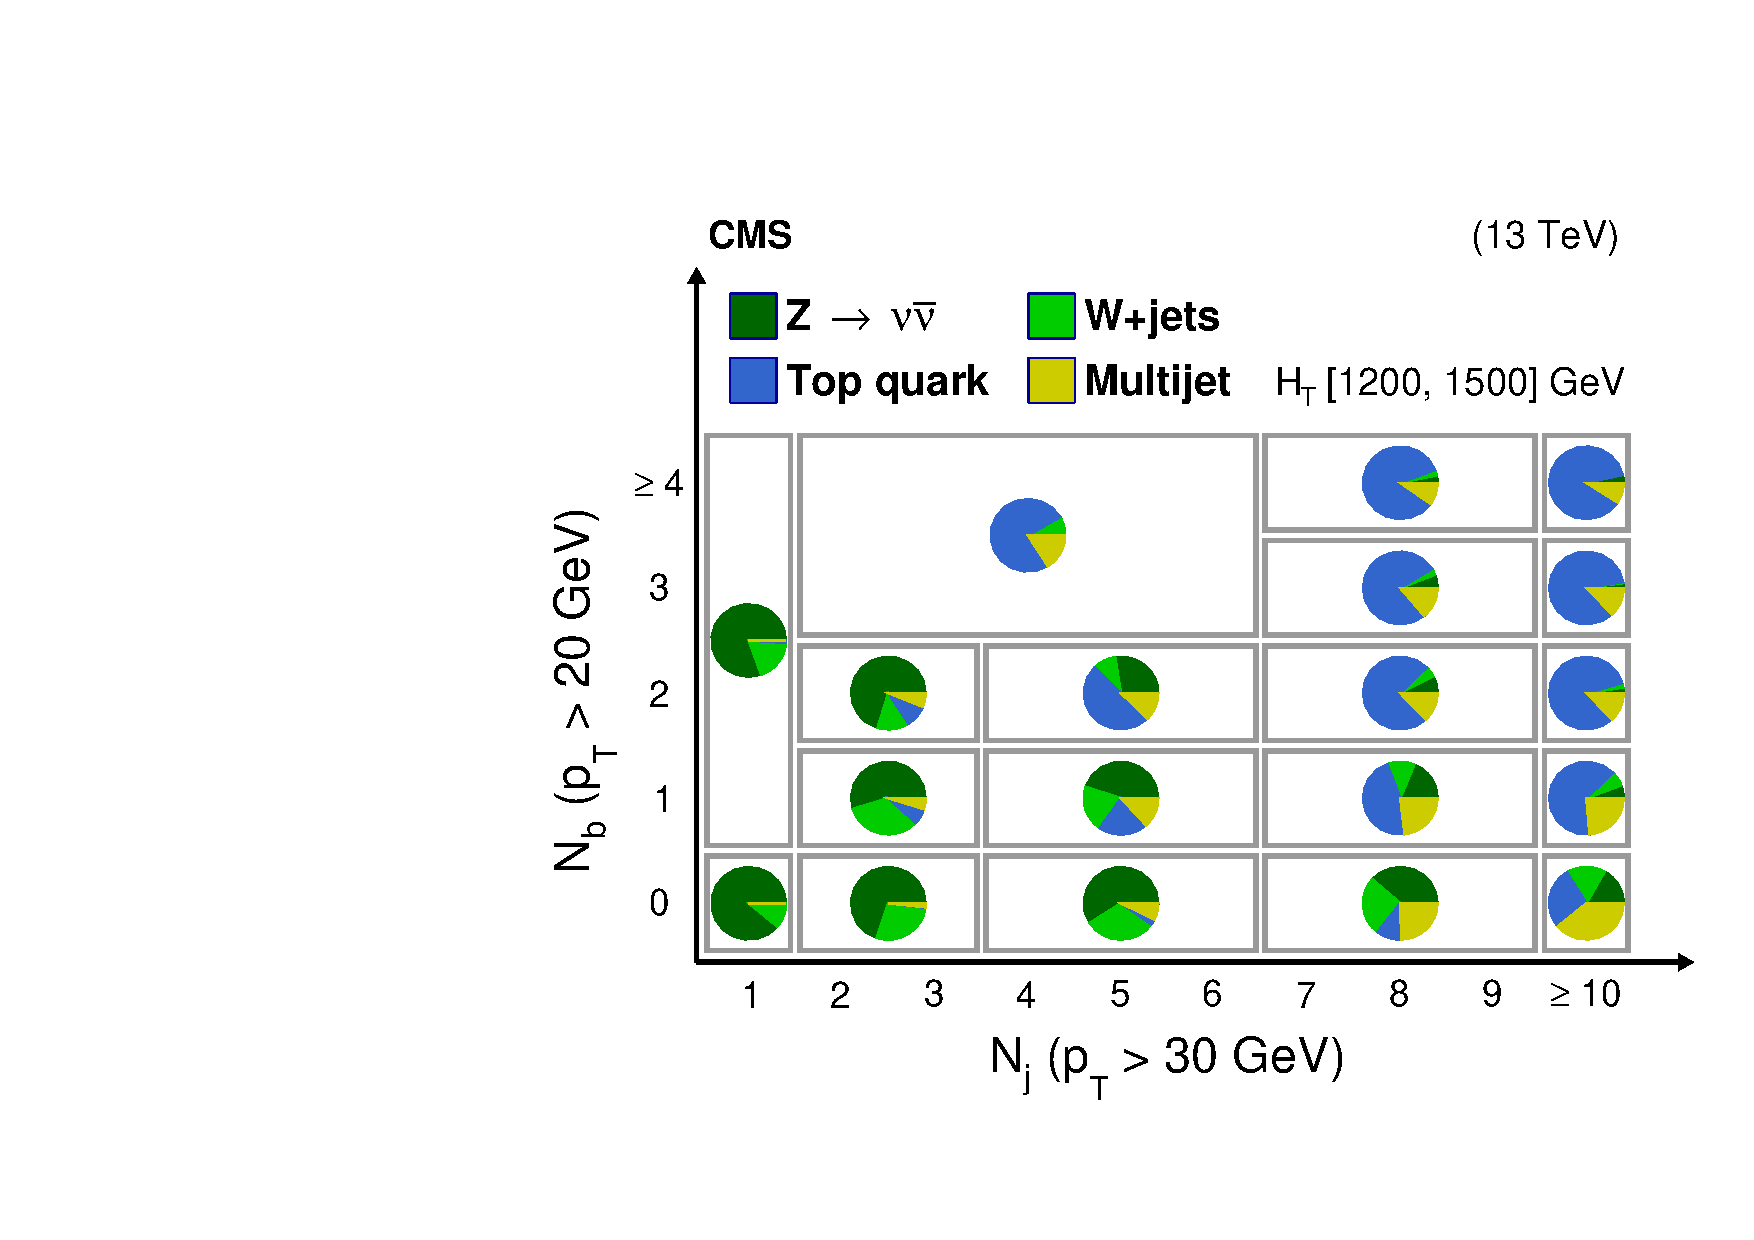
\includegraphics[width=0.8\textwidth]{figs/event_selection/piecharts_H.pdf}
    \caption{Topological region binning (defined by the solid gray lines)
      for the High \Ht region ($1200\leq\Ht<1500\GeV$). The proportion
      of each background type is shown as a pie chart in each topological region. QCD multijet becomes more imporant
      with increasing \Nj, and top backgrounds become more dominant at high \Nb. Background composition is estimated
      using the data-driven techniques described in the following chapters.
            }
    \label{fig:piechart_H}
  \end{center}
\end{figure}

Finally, we further divide each topological region into bins of \mttwo. The bin thresholds are chosen according
to the following criteria:
\begin{itemize}\setlength\itemsep{-1mm}
\item The lower edge of the first \mttwo bin is 200\GeV, except for $\Ht>1500$\GeV (Extreme \Ht) where it is 400\GeV.
\item In each topological region, we select the lower threshold of the last \mttwo bin such that this
bin is expected, from simulation, to contain approximately one background event. Moreover, the upper limit on \Ht
effectively places an upper limit on \mttwo. Therefore, this lower \mttwo threshold should not be larger than the upper limit
on \Ht, in each \Ht region.
\item Bin widths are nominally chosen to be 100\GeV. In each topological region, we merge \mttwo bins which are 
expected to contain less than one background event. In a few cases, we merge intermediate \mttwo bins
to minimize the number of signal region bins.
\end{itemize}

The final \mttwo binning for the multijet search regions can be found in 
Tables~\ref{tab:yieldsVL} through \ref{tab:yieldsUHh} in Appendix~\ref{app:yield_tables}

In addition to the $\Nj\geq2$ bins described above, we also select events with $\Nj=1$ (monojet), with the jet required to have
$\pt(\mrm{jet})>250\GeV$. Events are then categorized as follows:
\begin{itemize}\setlength\itemsep{-1mm}
\item Two \Nb regions: $\Nb=0$ and $\Nb\geq1$ (since the \pt threshold for \Nb is lower than that for \Nj, it
is possible that $\Nb>1$ even when $\Nj=1$)
\item For $\Nb=0$, \Ht bin edges of $[250,350,450,575,700,1000,1200,\infty]$\GeV
\item For $\Nb\geq1$, \Ht bin edges of $[250,350,450,575,700,\infty]$\GeV
\end{itemize}

In total, there are 270 multijet and 12 monojet regions for a total of 282 signal region search bins.

\section{Control regions}
\label{sec:crdefs}

To estimate the various backgrounds for this analysis, we make use of a number of control regions orthogonal 
to the signal region. These include a single lepton selection, a dileptonic selection (mostly \zll events), 
and a selection enriched in QCD multijet events.

\subsection{Single lepton control region}
\label{sec:crsl}
A single lepton selection is used to esimate backgrounds from \ttbar and \wjets (``lost lepton'' background).
The selection is the same as the baseline selection described in Sec.~\ref{sec:baselinesel}, with
the exception of the lepton veto. Instead, we require exactly one candidate passing the reconstructed lepton
or particle-flow lepton selections ($e$ or $\mu$ only). We further require this lepton candidate to satisfy
$M_\mrm{T}(\mrm{cand},\ptmiss)<100\GeV$ to reduce signal contamination. Events in which both the lepton
and missing energy are from leptonic $W$ decay tend to have $M_\mrm{T}\lesssim M_W=80\GeV$, while signal
events (in which the predominant source of \ptmiss is \emph{not} $W$ decay) tend to have much larger $M_\mrm{T}$.
As the \Ht and \ptmiss selections are the same as in the baseline signal region selection, 
the same triggers as used in the signal region are used for this single lepton control region.

When a true lepton is within detector acceptance, it is generally reconstructed in some form, even if
not classified as an isolated lepton candidate. We therefore remove the closest jet within
$\Delta R<0.4$ of the lepton candidate and count the lepton as a visible object for the purpose of computing
the variables \Ht, \Mht, \dphimet, $|\vMht-\vMet|/\ptmiss$, and \mttwo. The lepton is \emph{not} however used
in computing \Nj, as most leptons have low \pt.

The baseline single lepton control region is separated into $(\Ht,\Nj,\Nb)$ topological regions
in the same way as the signal region, with the exception of events with $\Nj\geq7$.
The regions with $\geq$7 jets and $\geq$1 b tag are all predicted using control region bins with 7--9 or $\geq$10 jets and 1--2 b tags
(but with the same \Ht binning as the signal regions).
This is motivated by the low control region statistics in bins with $\geq$10 jets or $\geq$7 jets and $\geq$2 b tags,
as well as potential signal contamination in bins with $\geq$7 jets and $\geq$3 b tags.
Similarly, regions with either 7--9 or $\geq$10 jets and 0 b tags are all predicted using control region bins
with $\geq7$ jets and 0 b tags, due to low control region statistics in bins with $\geq$10 jets.

The single lepton control region is not binned in \mttwo like the signal regions. Instead, the lost
lepton prediction along the \mttwo dimension is estimated using a hybrid technique described in 
Chapter~\ref{chap:lostlep}.

\subsection{Dilepton control regions}
\label{sec:dilep_cr}
We make use of two dilepton control regions: a same-flavor $e^\pm e^\mp/\mu^\pm\mu^\mp$ control region, consisting mostly
of \zll events and used to estimate the \znunu background, and an different-flavor $e^\pm\mu^\mp$
control region, used to estimate contamination from flavor-symmetric processes (mainly \ttbar)
in the same-flavor region.

In either case, we require two opposite-charge leptons passing the reconstructed lepton selections
given in Secs.~\ref{sec:electrons} and \ref{sec:muons}. Dileptonic triggers are used, 
and to improve trigger efficiency we further
require that electrons pass a slightly tigher cut-based ID requirement (``loose'' instead of ``veto'').
The leptons must satisfy $\pt(\ell\ell)>200\GeV$ (to ensure similar kinematics to high-\pt \znunu
events that populate the signal regions), and leading/subpleading lepton $\pt>100/35\GeV$. The invariant
mass $m_{\ell\ell}$ must satisfy $|m_{\ell\ell}-m_Z|<20\GeV$ in order to ensure we select mainly $Z$ events.

Since the leptons take the place of the neutrinos in \znunu events, to emulate the kinematics the
lepton \vSS{p}{T}{} vectors are added to the \vMet vector for use in the computation of all
kinematic variables. Further, since leptons are usually reconstucted as (at least components of) jets,
the closest jet within $\Delta R<0.4$ of each lepton is removed from the event before computing kinematic
quantities. The variables \Nj, \Nb, \Ht, \Mht, \dphimet, $|\vMht-\vMet|/\ptmiss$, and \mttwo are all
potentially modified by these changes.

In addition to the main same-flavor and different-flavor control regions described above, there is
additionally an auxilliary different-flavor region enriched in \ttbar, used to measure the ratio
of same-flavor to different-flavor events from flavor-symmetric processes. This is defined by
inverting the $\pt(\ell\ell)$ and $m_{\ell\ell}$ selections, so that $\pt(\ell\ell)<200\GeV$
and $|m_{\ell\ell}-m_Z|>20\GeV$.

Similarly as for the single lepton control region, the dilepton control region is binned into
topological in the same way as the signal region, with the exception of bins with $\geq$7 jets.
This time, signal regions with 7--9 or $\geq$10 jets and 0 b tags are predicted with control
region bins with $\geq$7 jets and 0 b tags, and signal regions with 7--9 or $\geq$10 jets and
$\geq$ 1 b tag are predicted using control regions with $\geq$ 7 jets and $\geq$ 1 b tag
(still with the same \Ht binning as the signal regions).

\subsection{QCD-enriched control regions}
We define a few control regions orthogonal to the signal region that are enriched in
QCD multijet events, in order to validate the estimate of the QCD multijet background.
This is done by inverting cuts on the two kinematic variables mainly responsible for
rejecting QCD background. The baseline signal region selection is applied, with the
exception of one of the following:
\begin{itemize}\setlength\itemsep{-1mm}
\item the \dphimet requirement is inverted to $\dphimet<0.3$.
\item the \mttwo requirement is shifted to $100<\mttwo<200\GeV$
\item \emph{both} the \dphimet and \mttwo cuts are changed as above
\end{itemize}
%
The same triggers are used as in the signal regions.

\section{2018 HEM 15/16 failure}
\label{sec:hem}

During 2018 data taking, two modules in the minus-side HCAL endcap (HEM), 
representing about a 45$^\circ$ angle, were lost.
This means that any energy deposited in these modules was not recorded.
The effects of this are (1) under-measured jets in the region,
as a fraction of the energy is lost, and (2) increased electron and
photon fake rates, as jets in the region have inflated EM-to-hadronic
energy ratios.

Studies showed this has negligible impact on backgrounds with real \ptmiss
(i.e. invisible $Z$ and lost lepton), but a significant effect
on the fake-\ptmiss QCD multijet background.  Fig.~\ref{fig:hem} shows
on the left the actual observed effect on an imbalanced dijet control region,
and on the right the estimated effect on QCD yields in the signal regions,
found by modifying the Rebalance \& Smear method with special HEM response
functions measured in HEM-emulated data. Up to an 8-fold increase in QCD
background is observed.
Additionally, we observed an excess of events in the single lepton
control region with the single lepton being a fake electron in the HEM region.

To avoid contaminating our signal and control regions with these HEM-affected events,
we apply a special veto to the affected portion of 2018 data,
as well as a fraction of the 2018 MC events corresponding to the
fraction of affected data (about 39 out of 58 fb$^{-1}$, or 66\%).
The filter rejects events containing certain objects in the HEM region, defined
as $\eta\in[-4.7,-1.4]$ and $\phi\in[-1.6,-0.8]$.
The objects that trigger the veto are as follows:
\begin{itemize}\setlength\itemsep{-1mm}
\item For events with $\Nj=1$ or $\Ht<575\GeV$, any jet with $\pt>20\GeV$.
\item Also for events with $\Nj=1$ or $\Ht<575\GeV$, any lost track with $d_z<0.2$ cm
and $d_{xy}<0.1$ cm (a ``lost track'' is any track not reconstructed as a PF candidate).
\item For events with $\Nj\geq2$ and $\Ht\geq575\GeV$, any jet with $\pt>30\GeV$.
\item The electron for any events in the single lepton control region.
\end{itemize}

\begin{figure}[t]
  \begin{center}
    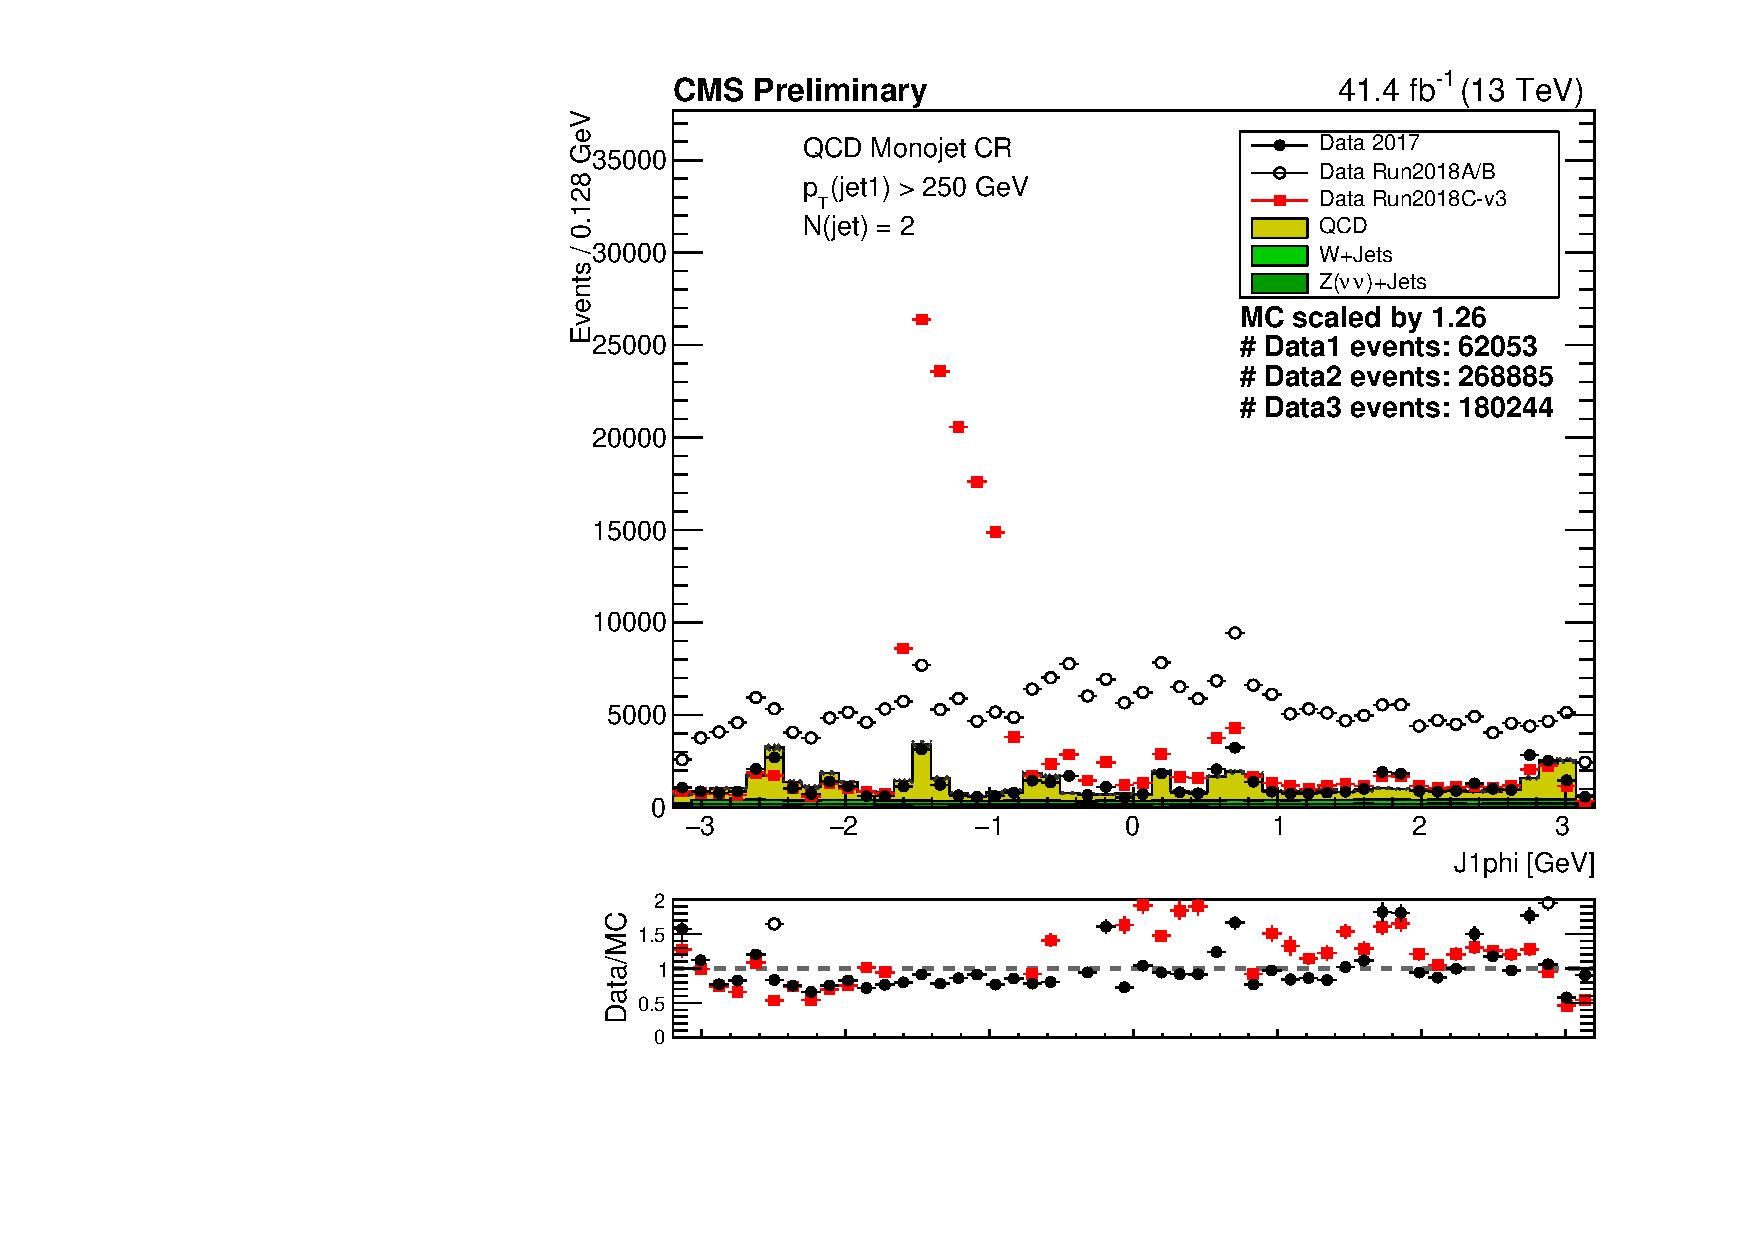
\includegraphics[width=0.42\textwidth]{figs/event_selection/hem_subleadjetphi.pdf}
    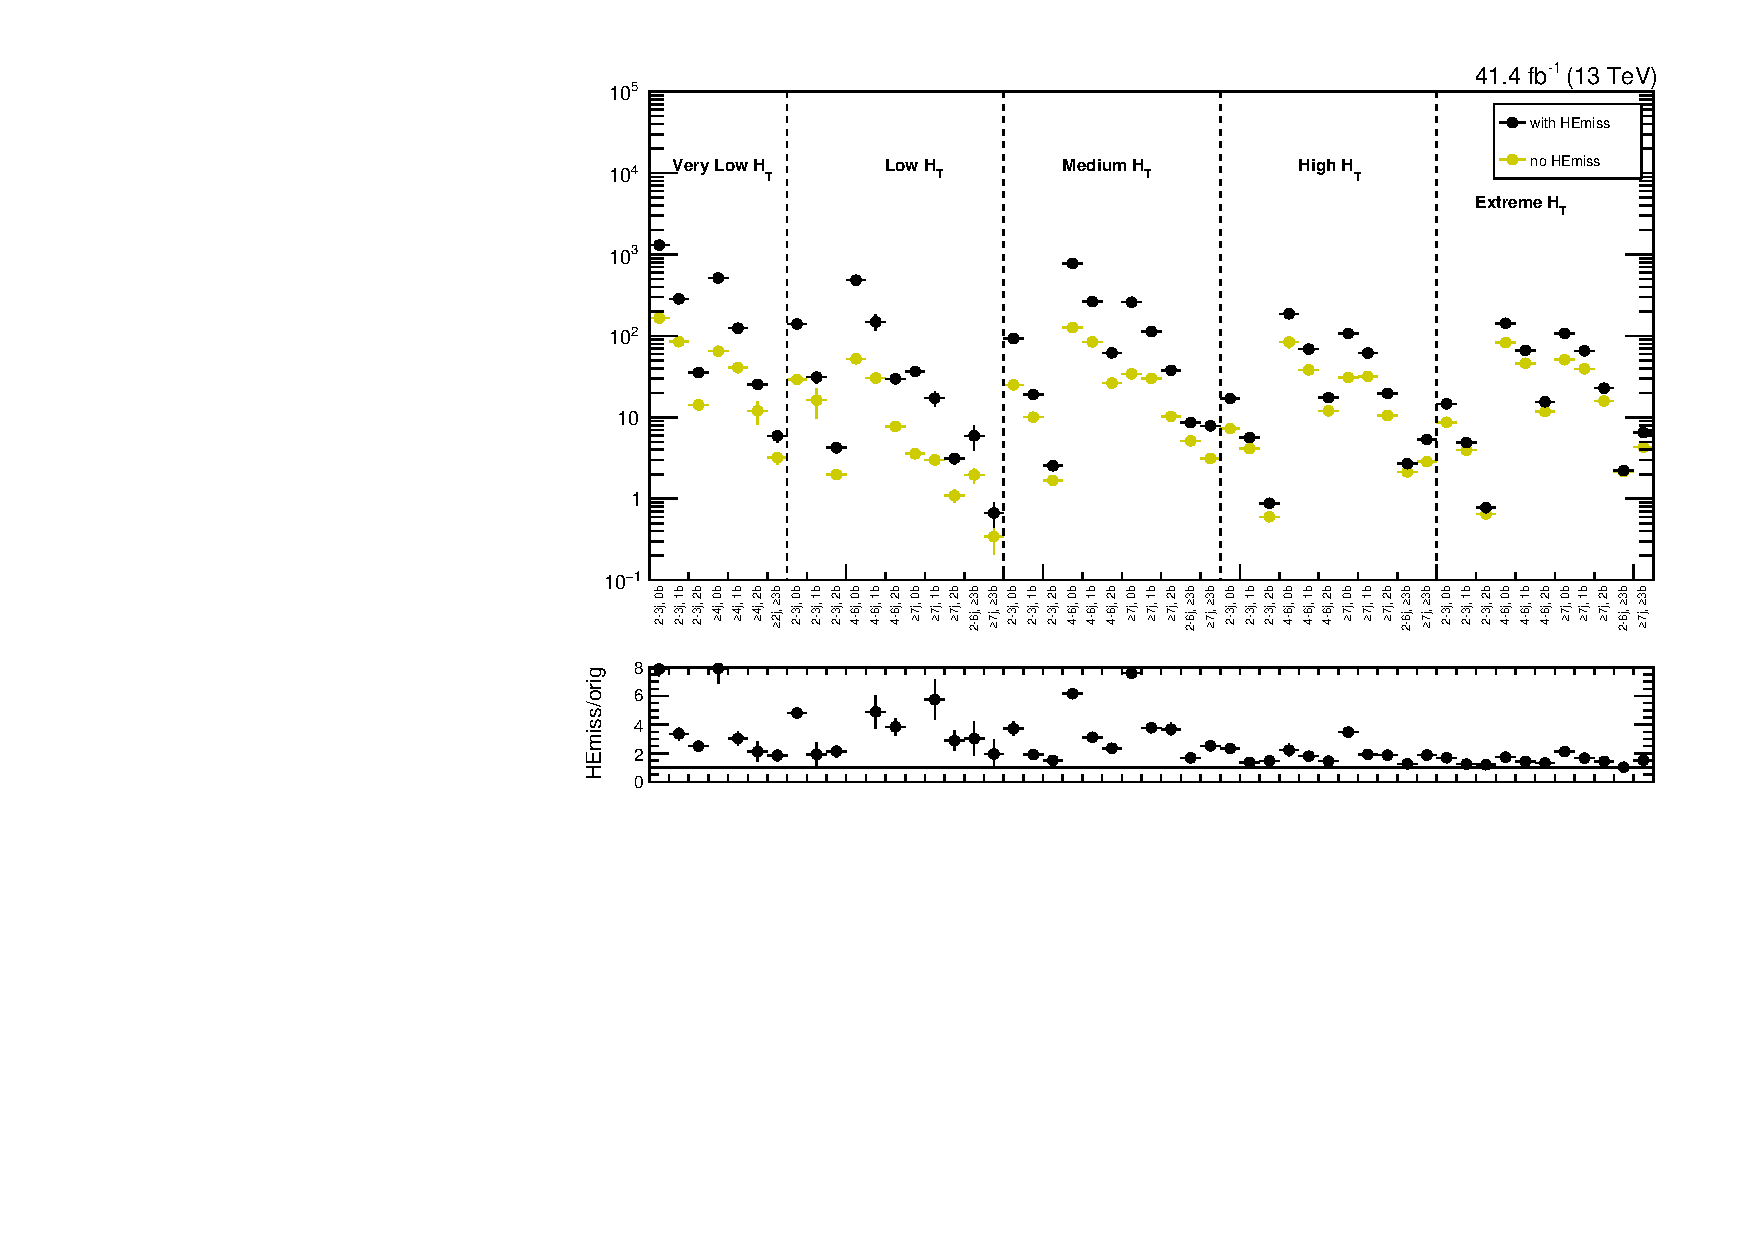
\includegraphics[width=0.57\textwidth]{figs/event_selection/mc_closure_sr.pdf}
    \caption{(left) Sub-leading jet $\phi$ before and after the HEM issue.
      Black points are 2017, and are flat in $\phi$ and agree with MC. White
      points are early pre-HEM issue 2018 data, flat in $\phi$ but with 
      a uniform excess due to an unrelated filter issue that was since fixed.
      Red points are post-HEM issue 2018 data, showing a clear excess in the HEM region
      $\phi\in[-1.6,0.8]$. Dijet events that are otherwised balanced but have a jet in
      the HEM region become imbalanced due to the lost energy.
      (right) Estimated effect of HEM issue on QCD signal region yields, found by 
      modifying Rebalance \& Smear templates with special response functions measured
      in HEM-emulated data. The issue causes up to an 8-fold increase in estimated
      background, and the effect is worst at low \Ht.
            }
    \label{fig:hem}
  \end{center}
\end{figure}

\chapter{Invisible Z Background}
\label{chap:zinv}

One of the main sources of background to the \mttwo analysis comes from the production of a $Z$
boson in association with one or more jets, where the $Z$ decays ``invisibly'' to two neutrinos.
This is an \emph{irreducible} background, since the signature is exactly like that of signal:
no prompt charged leptons, real \ptmiss, and multiple jets. For signal models that produce
b quarks, however, the number of b-tagged jets becomes a discriminating variable as there are
no inherent b jets in \zjets production.

To estimate this background in a data-driven way, we make use of the fact that $Z$ bosons may also decay into two
charged leptons with known branching fraction. The rate of \zll production is measured in data, and this is
translated into an estimate on \znunu by multiplying by a transfer factor derived from Monte Carlo.
Section~\ref{sec:znunu_from_zll} describes how this is done in each $(\Ht,\Nj,\Nb)$ topological region,
Sec.~\ref{sec:zinv_mt2} details the ``hybrid template'' method for extrapolating the estimate along the
\mttwo dimension, and Sec.~\ref{sec:zinv_syst} describes the systematic uncertainties assessed on the 
final estimate.

\section{Estimating \texorpdfstring{\znunu}{Z\unichar{"2192}\unichar{"03BD}\unichar{"03BD}} from \texorpdfstring{\zll}{Z\unichar{"2192}ll}}
\label{sec:znunu_from_zll}
The exact definition of the dilepton control region used in the \znunu estimate is described in Sec.~\ref{sec:dilep_cr}.
It is constructed to be enriched in \zll events (as opposed to other dilepton-producing processes, such as \ttbar),
and the lepton \vSS{p}{T}{} vectors are added to the \vMet in order to mimic the kinematics of \znunu events.

Data vs.\ MC comparisons of the main analysis kinematic variables in the baseline \zll control region are 
shown in Fig.~\ref{fig:zll_crplots}. There is some level of disagreement between data and MC, but this is
to be expected. The estimate is primarily data-driven, and MC is used only at leading order, so these
disagreements generally do not affect the final estimate. Where MC is used, primarily in the far
\mttwo tails, appropriate systematic uncertainties are assigned.

\begin{figure}[htbp]
  \begin{center}
    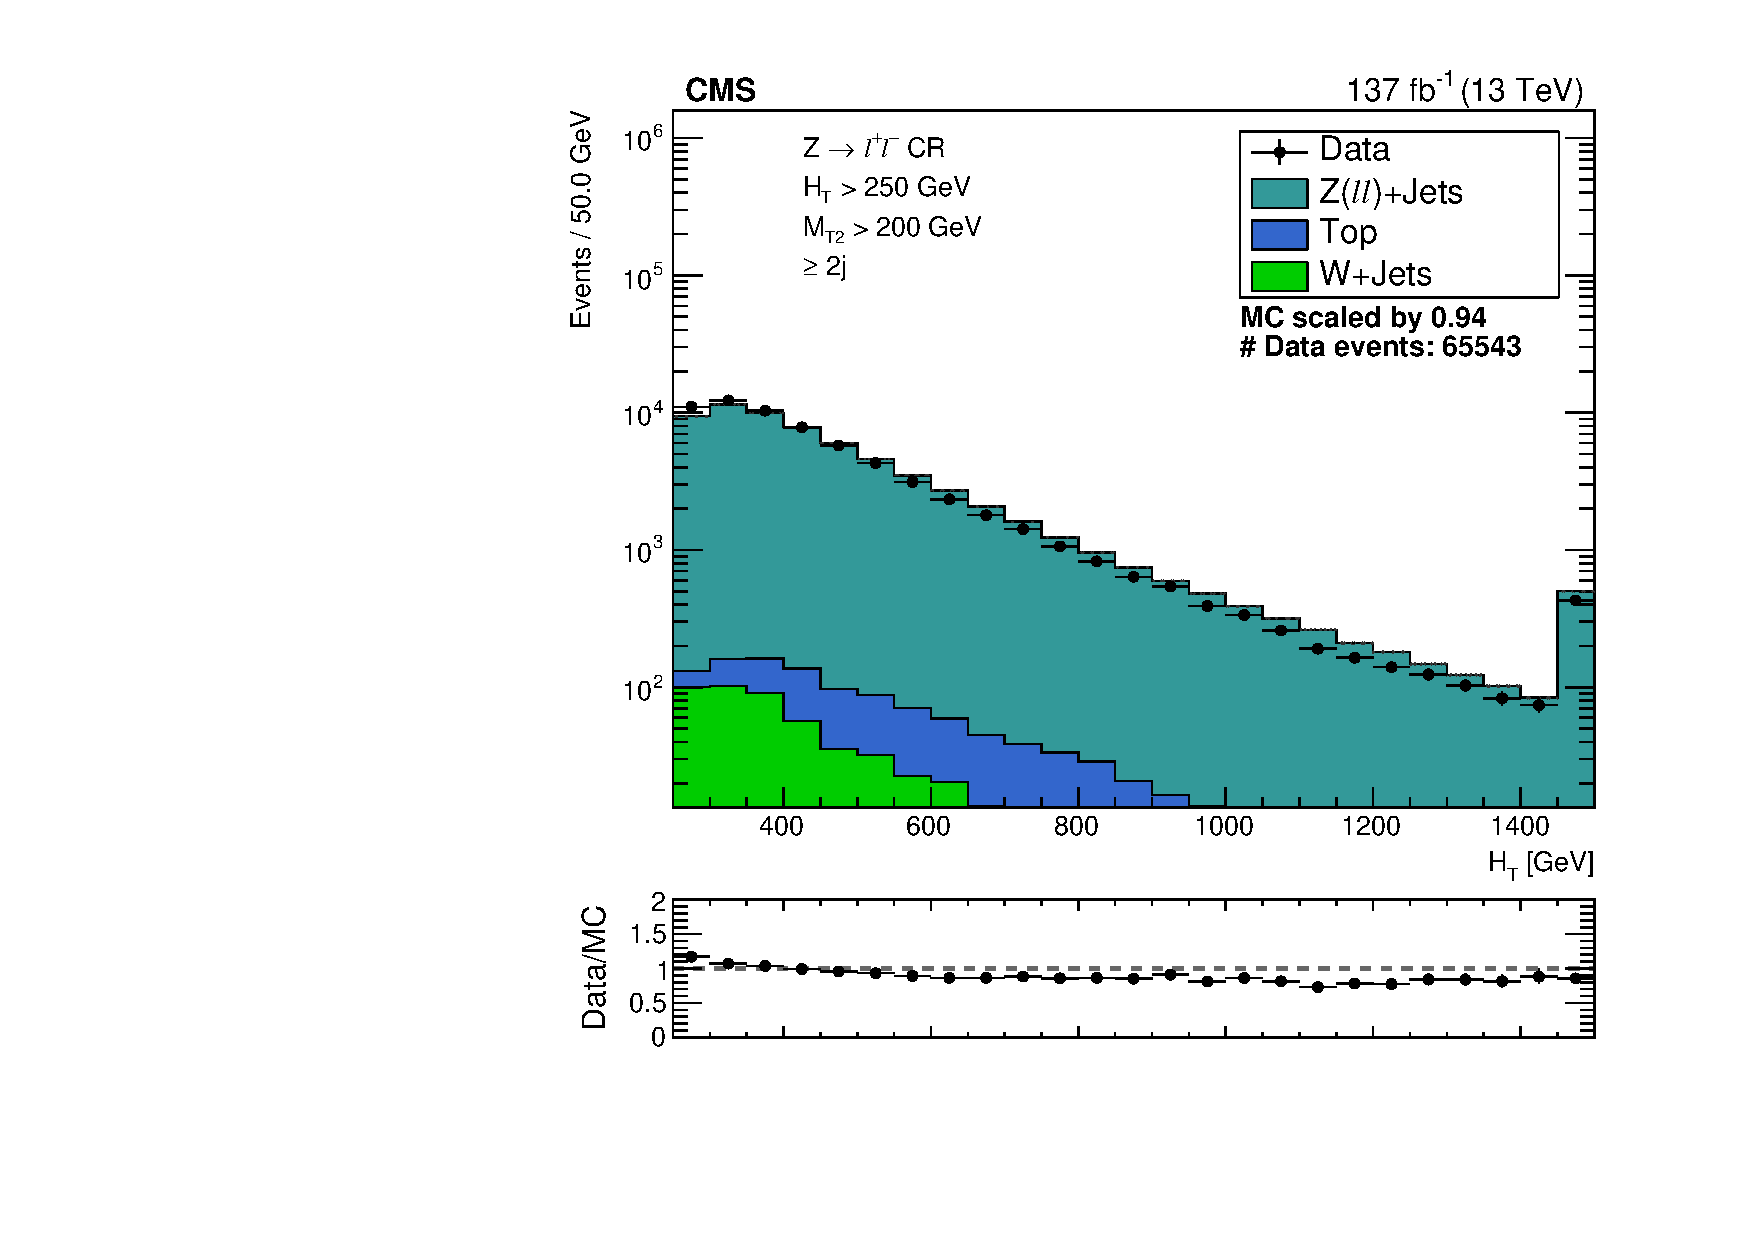
\includegraphics[width=0.47\textwidth]{figs/zinv/crdybase_ht.pdf}
    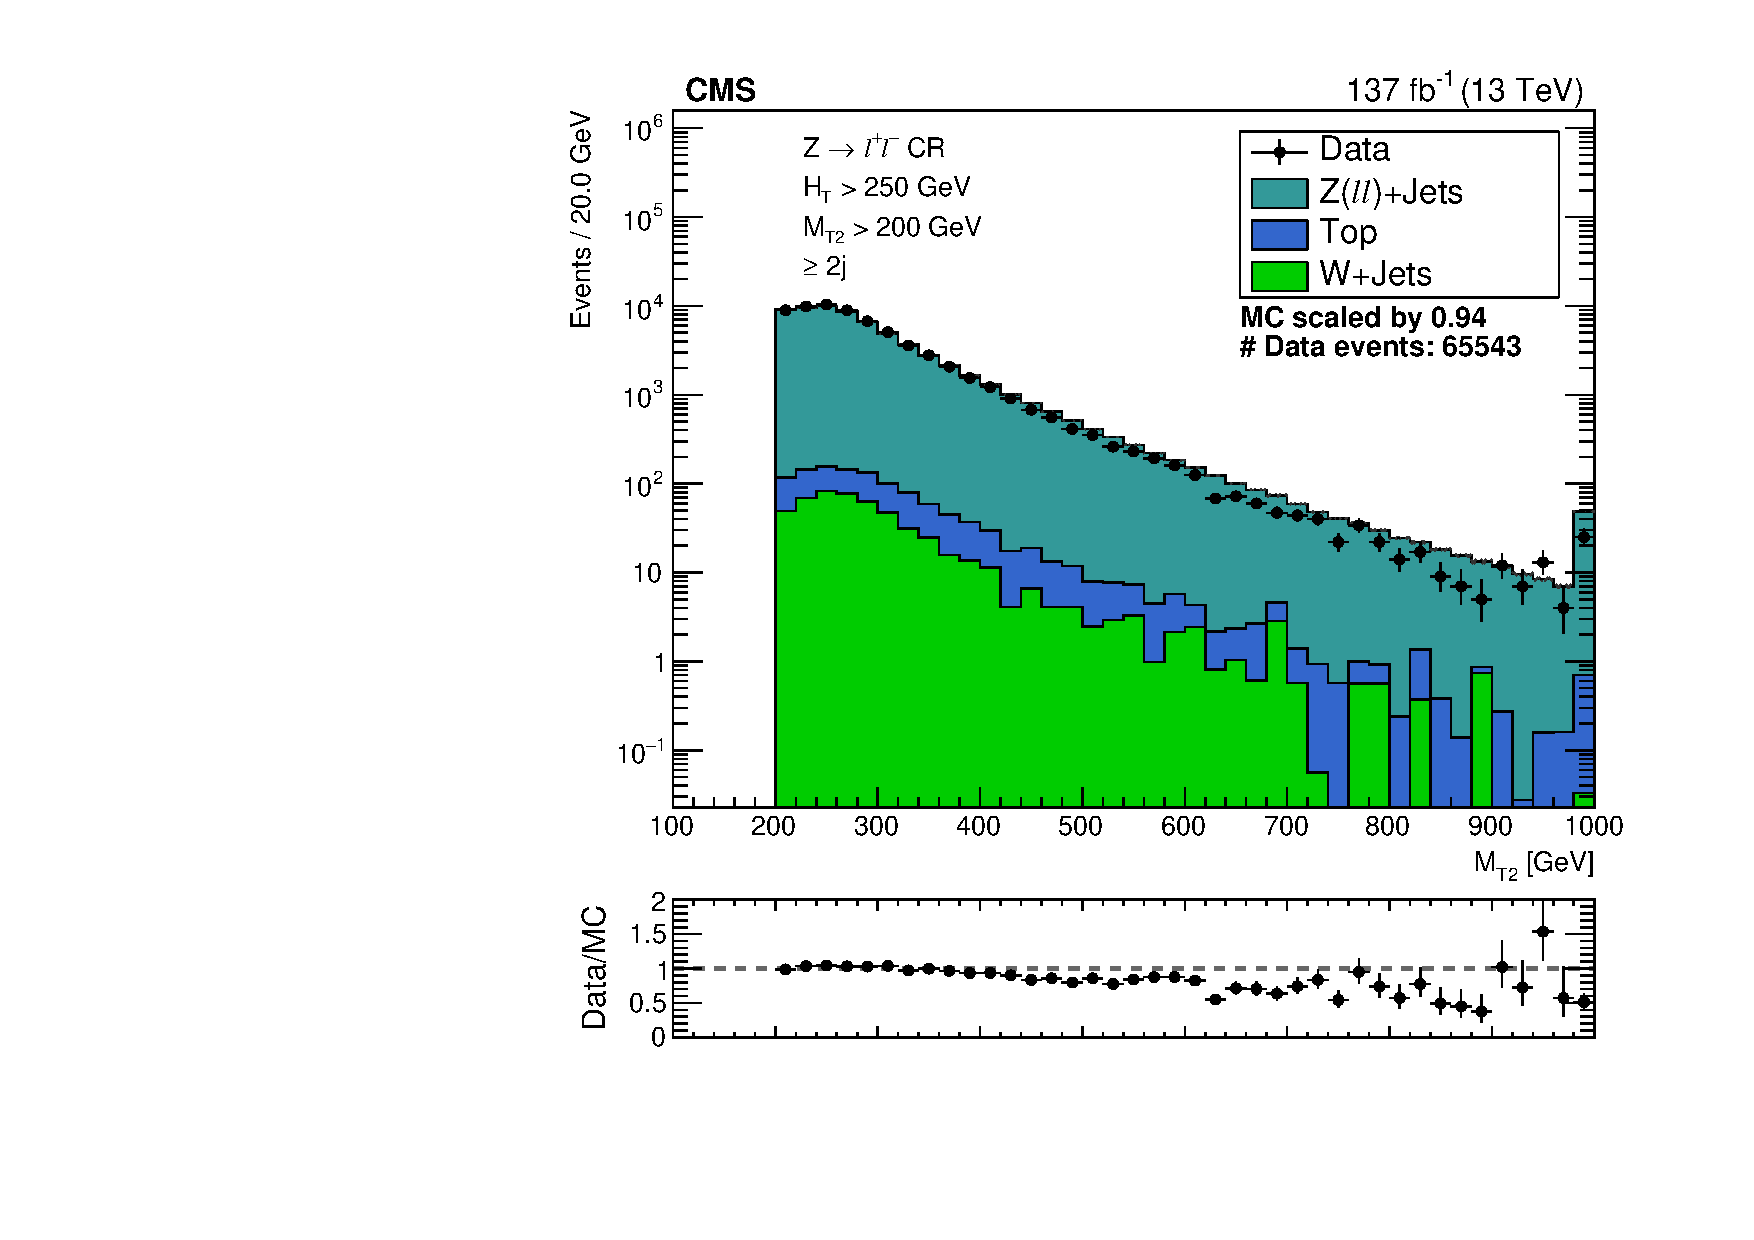
\includegraphics[width=0.47\textwidth]{figs/zinv/crdybase_mt2.pdf} \\
    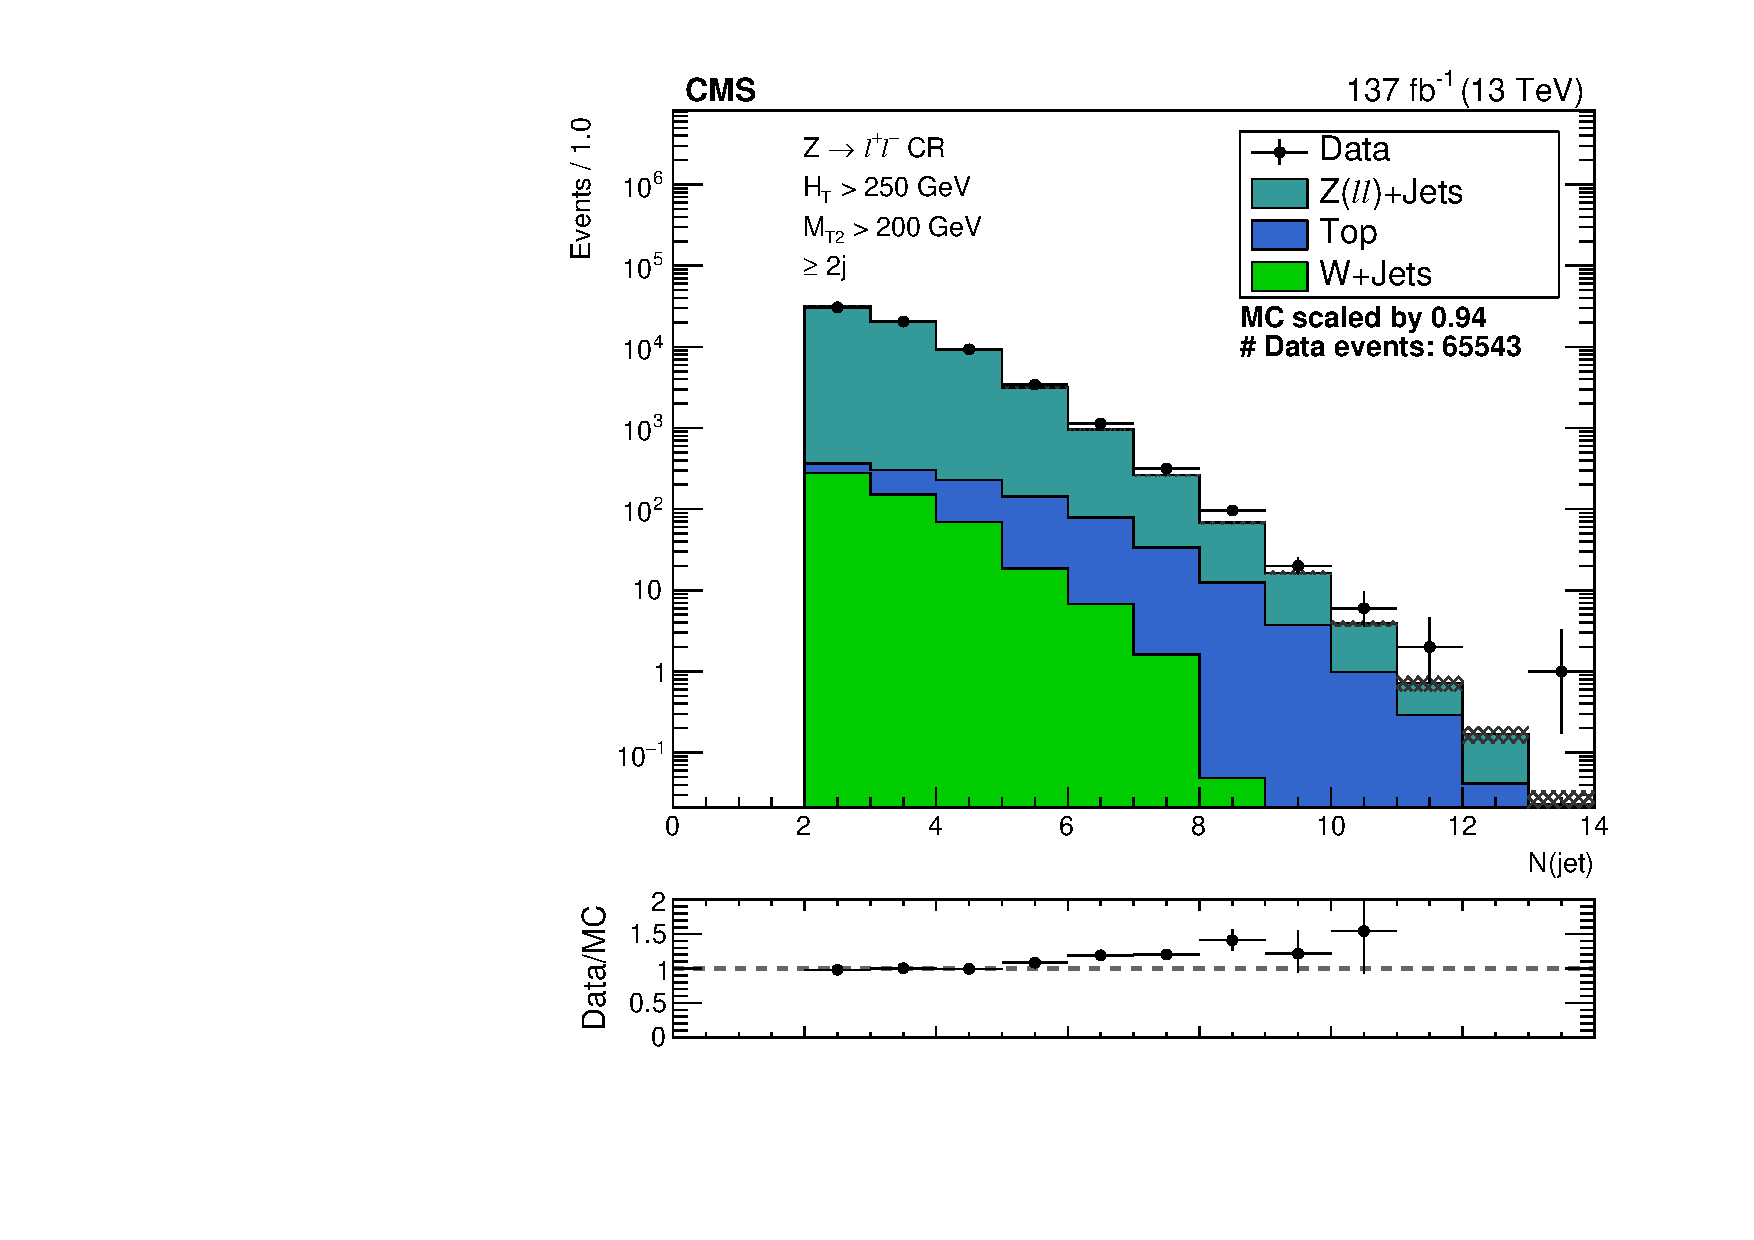
\includegraphics[width=0.47\textwidth]{figs/zinv/crdybase_nJet30.pdf}
    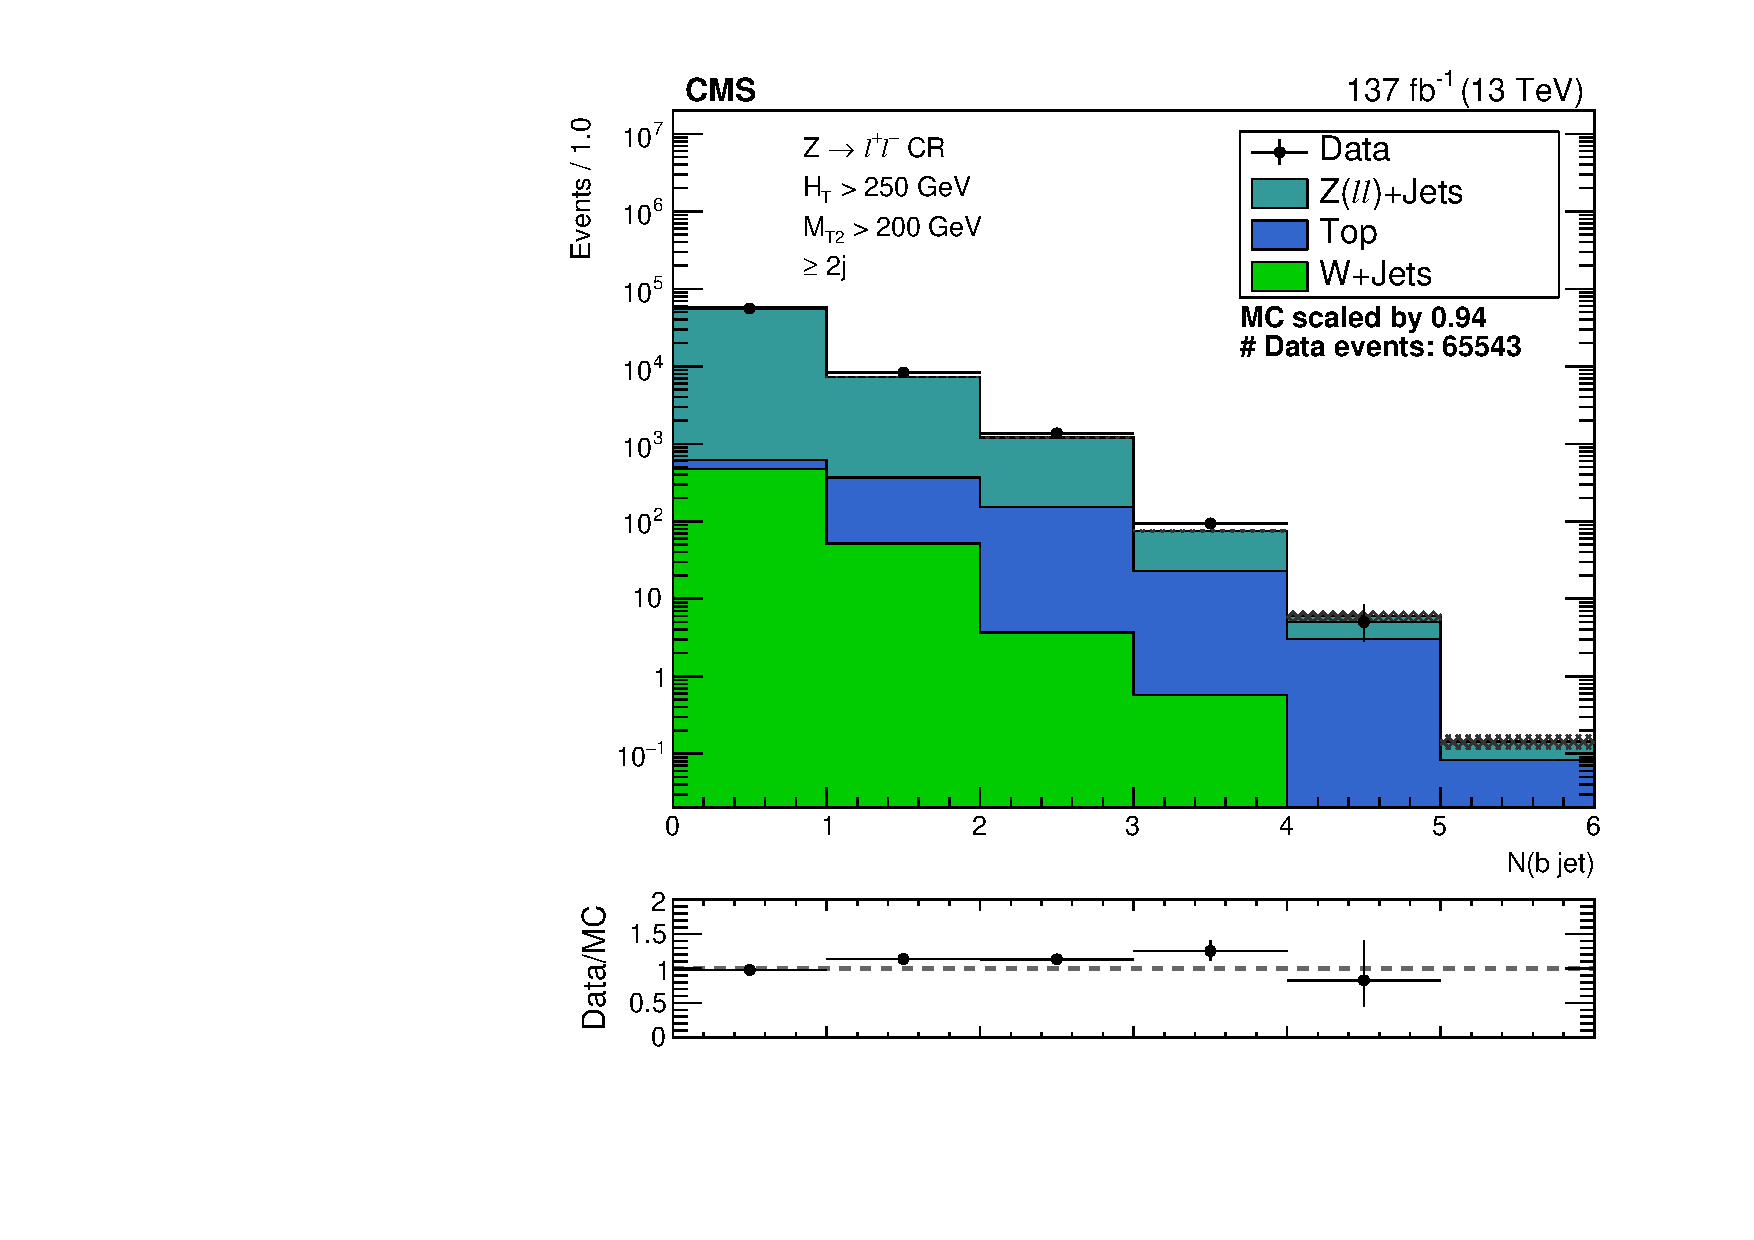
\includegraphics[width=0.47\textwidth]{figs/zinv/crdybase_nBJet20.pdf} \\
    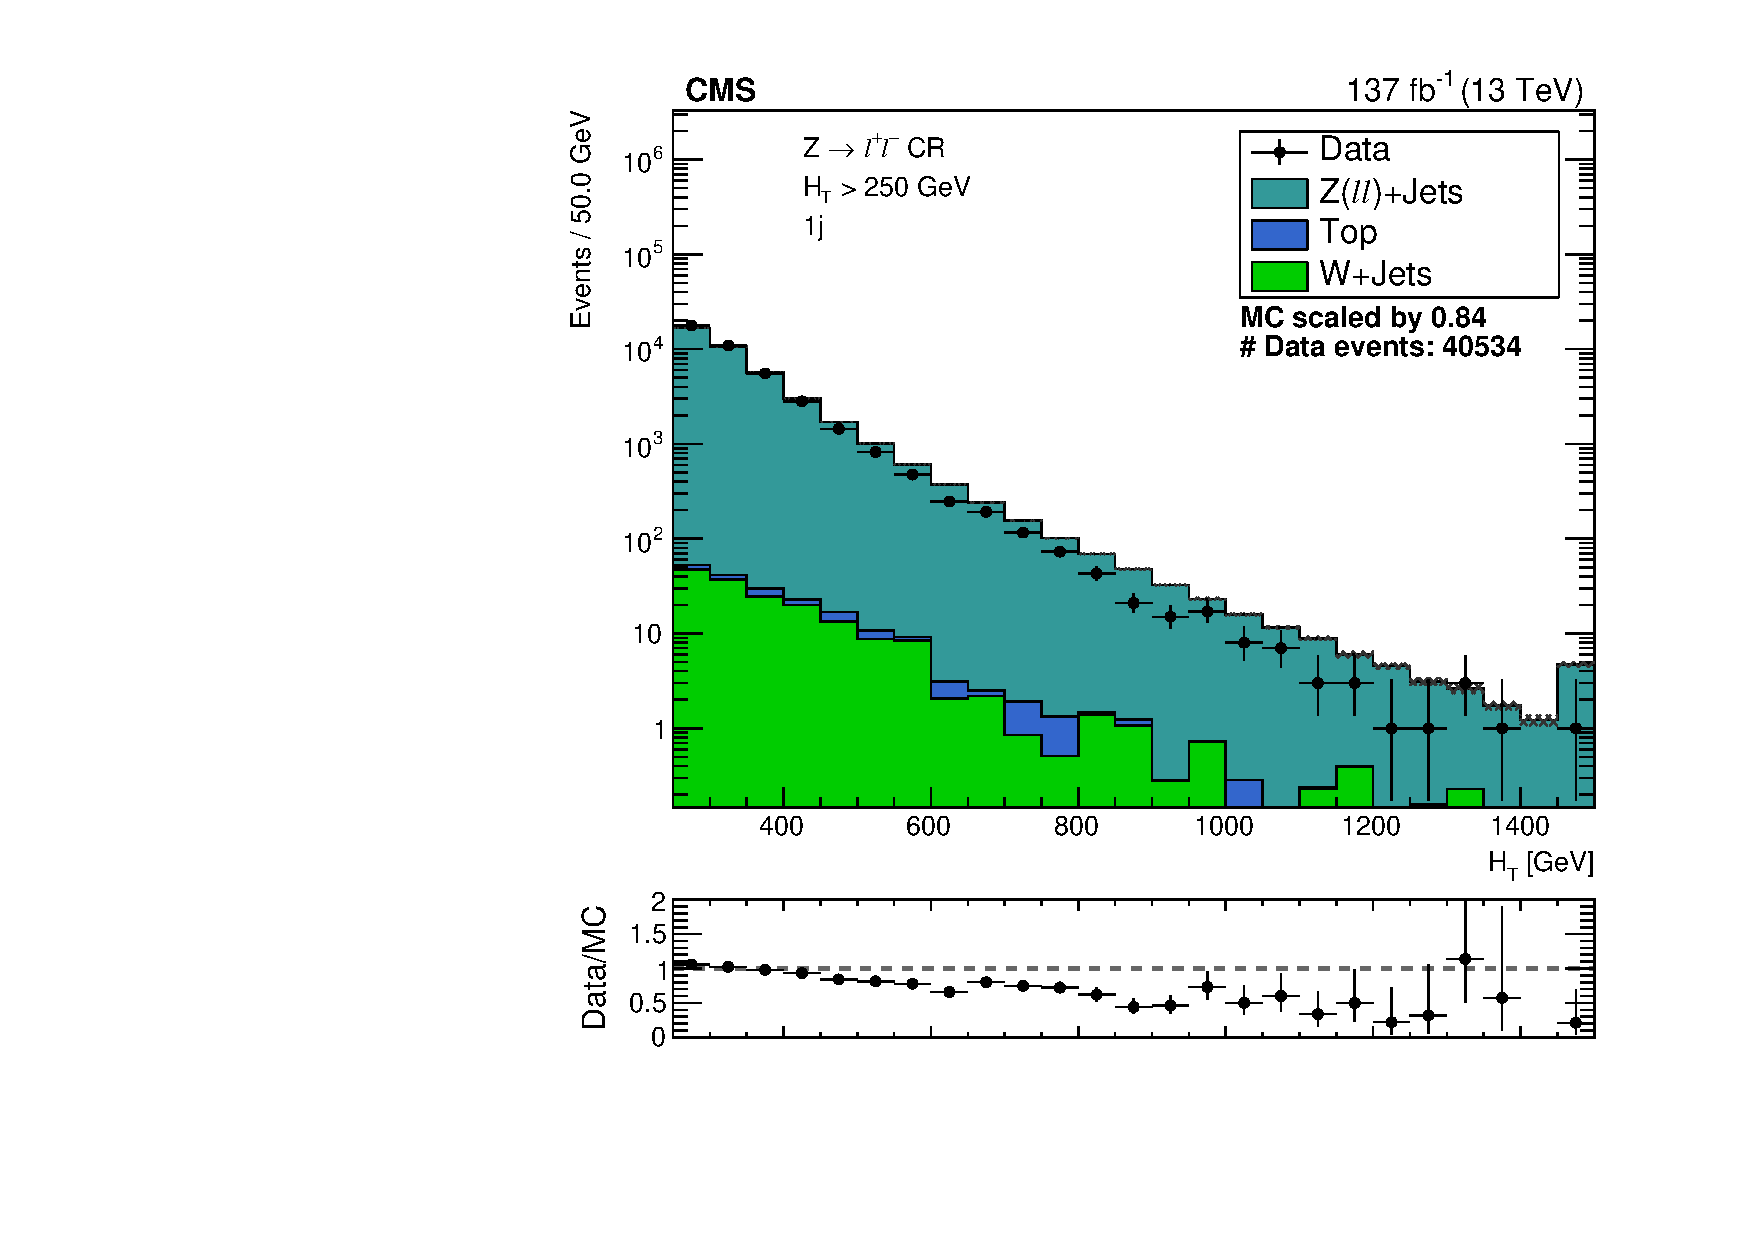
\includegraphics[width=0.47\textwidth]{figs/zinv/crdybaseJ_ht.pdf}
    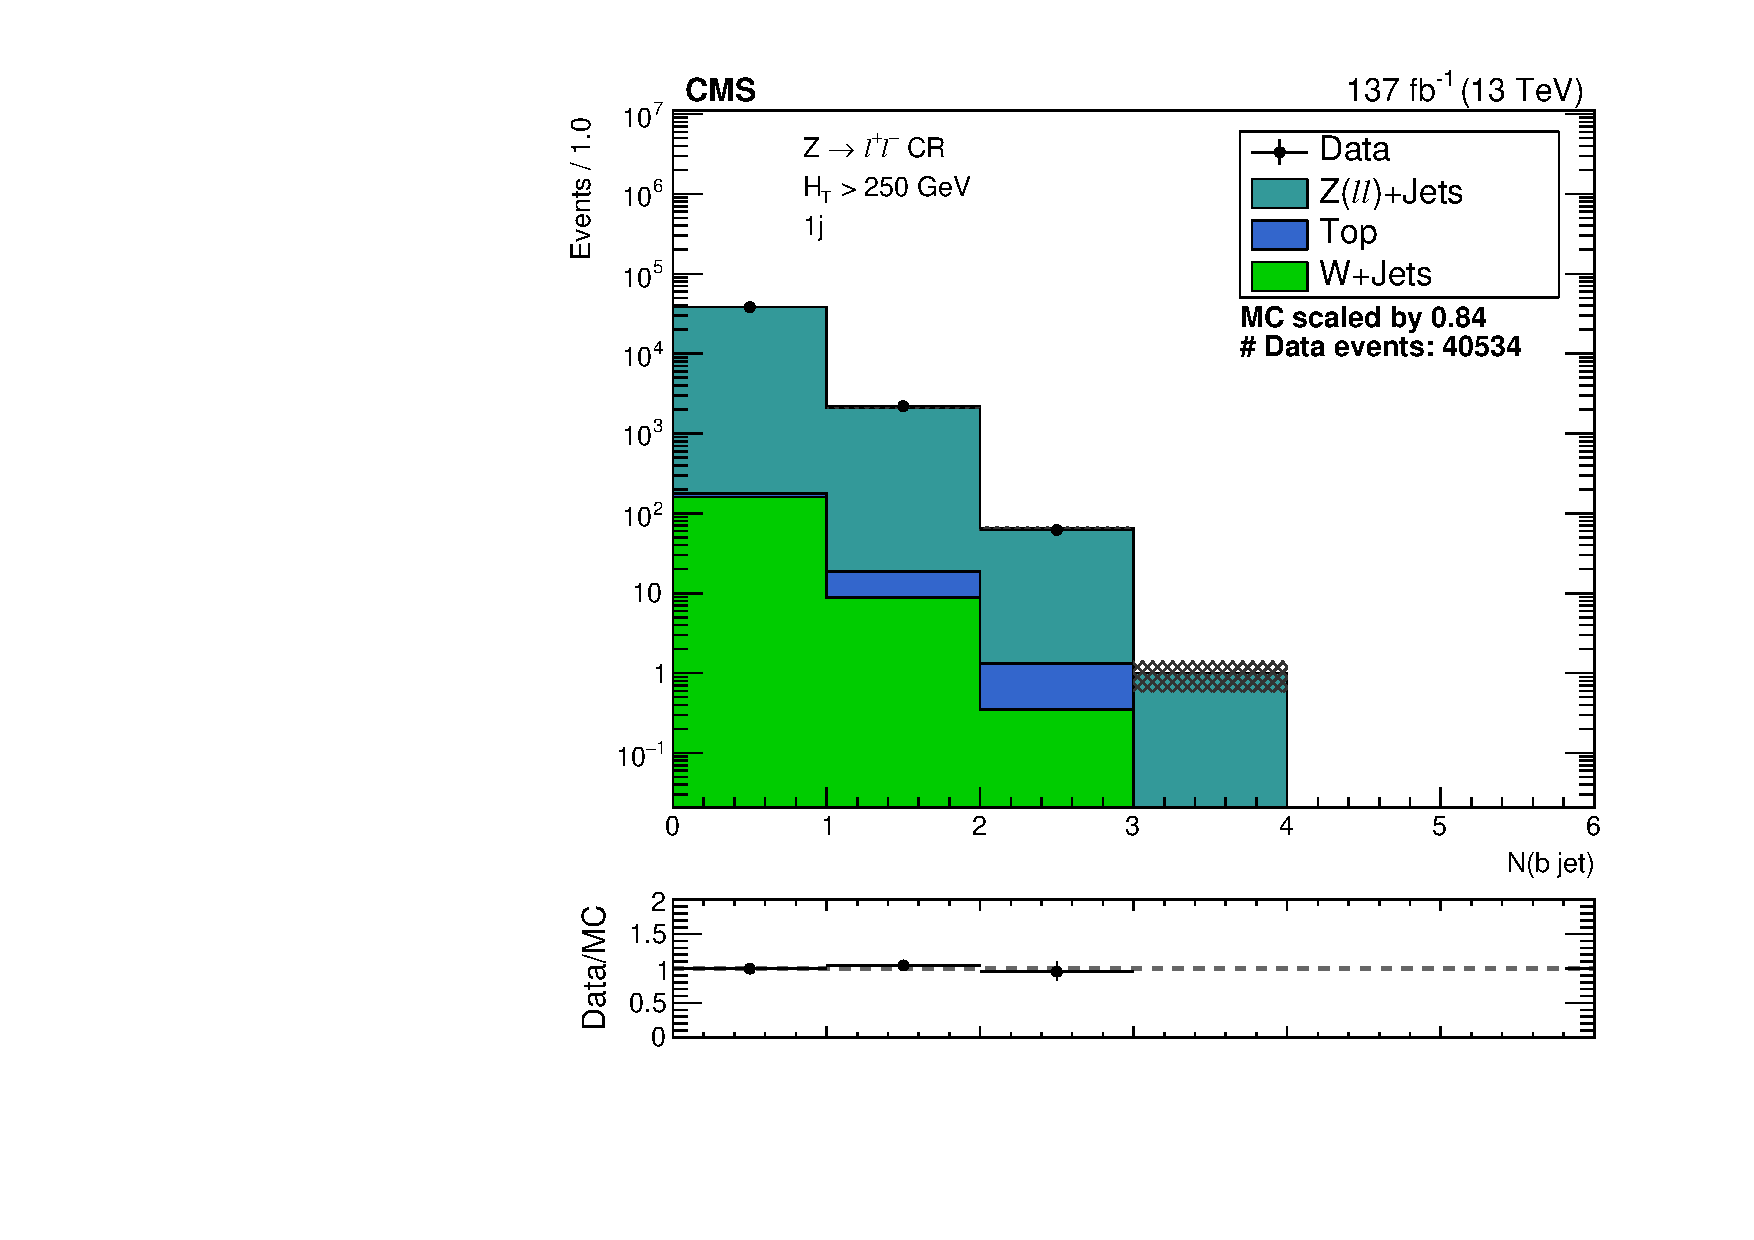
\includegraphics[width=0.47\textwidth]{figs/zinv/crdybaseJ_nBJet20.pdf}
    \caption{Data vs.\ MC comparisons in the baseline \zll control region, for $\Nj\geq2$
      (top two rows), and $\Nj=1$ (bottom row). From left to right, top to bottom, the variables
      plotted are \Ht, \mttwo, \Nj, \Nb, \Ht, and \Nb.
            }
    \label{fig:zll_crplots}
  \end{center}
\end{figure}

The \znunu estimate is first performed in each $(\Ht,\Nj,\Nb)$ topological region, integrated
over \mttwo (for the monojet region, the \Ht dimension is equivalent to $\vSS{p}{T}{\mrm{jet1}}$,
so there is no integration and the estimate is performed in each analysis bin). For all regions
with $\geq$7 jets and $\geq$1 b tag, an inclusive control region with $\geq$7 jets and $\geq$1 b tag
is used, to avoid statistical fluctuations in these regions where \znunu is a subleading background.
Similarly, for regions with 7--9 jets or $\geq$10 jets and 0 b tags, an inclusive control region
with $\geq$7 jets and 0 b tags is used. Since MC is used directly to predict the \Nj and \Nb
shapes here, agreement between data and MC is explicitly checked in these high-\Nj regions.
Fig.~\ref{fig:zll_ge7j} shows data vs.\ MC comparisons of \Nj and \Nb in the $\geq$7 jet region;
sufficient agreement is seen to justify the use of MC in predicting the \Nj and \Nb shapes.

For regions with $\Ht>1500\GeV$, all events with
$\mttwo>200\GeV$ are used in the control region even though the signal region starts at $\mttwo>400\GeV$.
Once the per-topological region estimate is done, a hybrid approach using both data and MC is
used to extrapolate along the \mttwo dimension, as described in Sec.~\ref{sec:zinv_mt2}.

\begin{figure}[ht]
  \begin{center}
    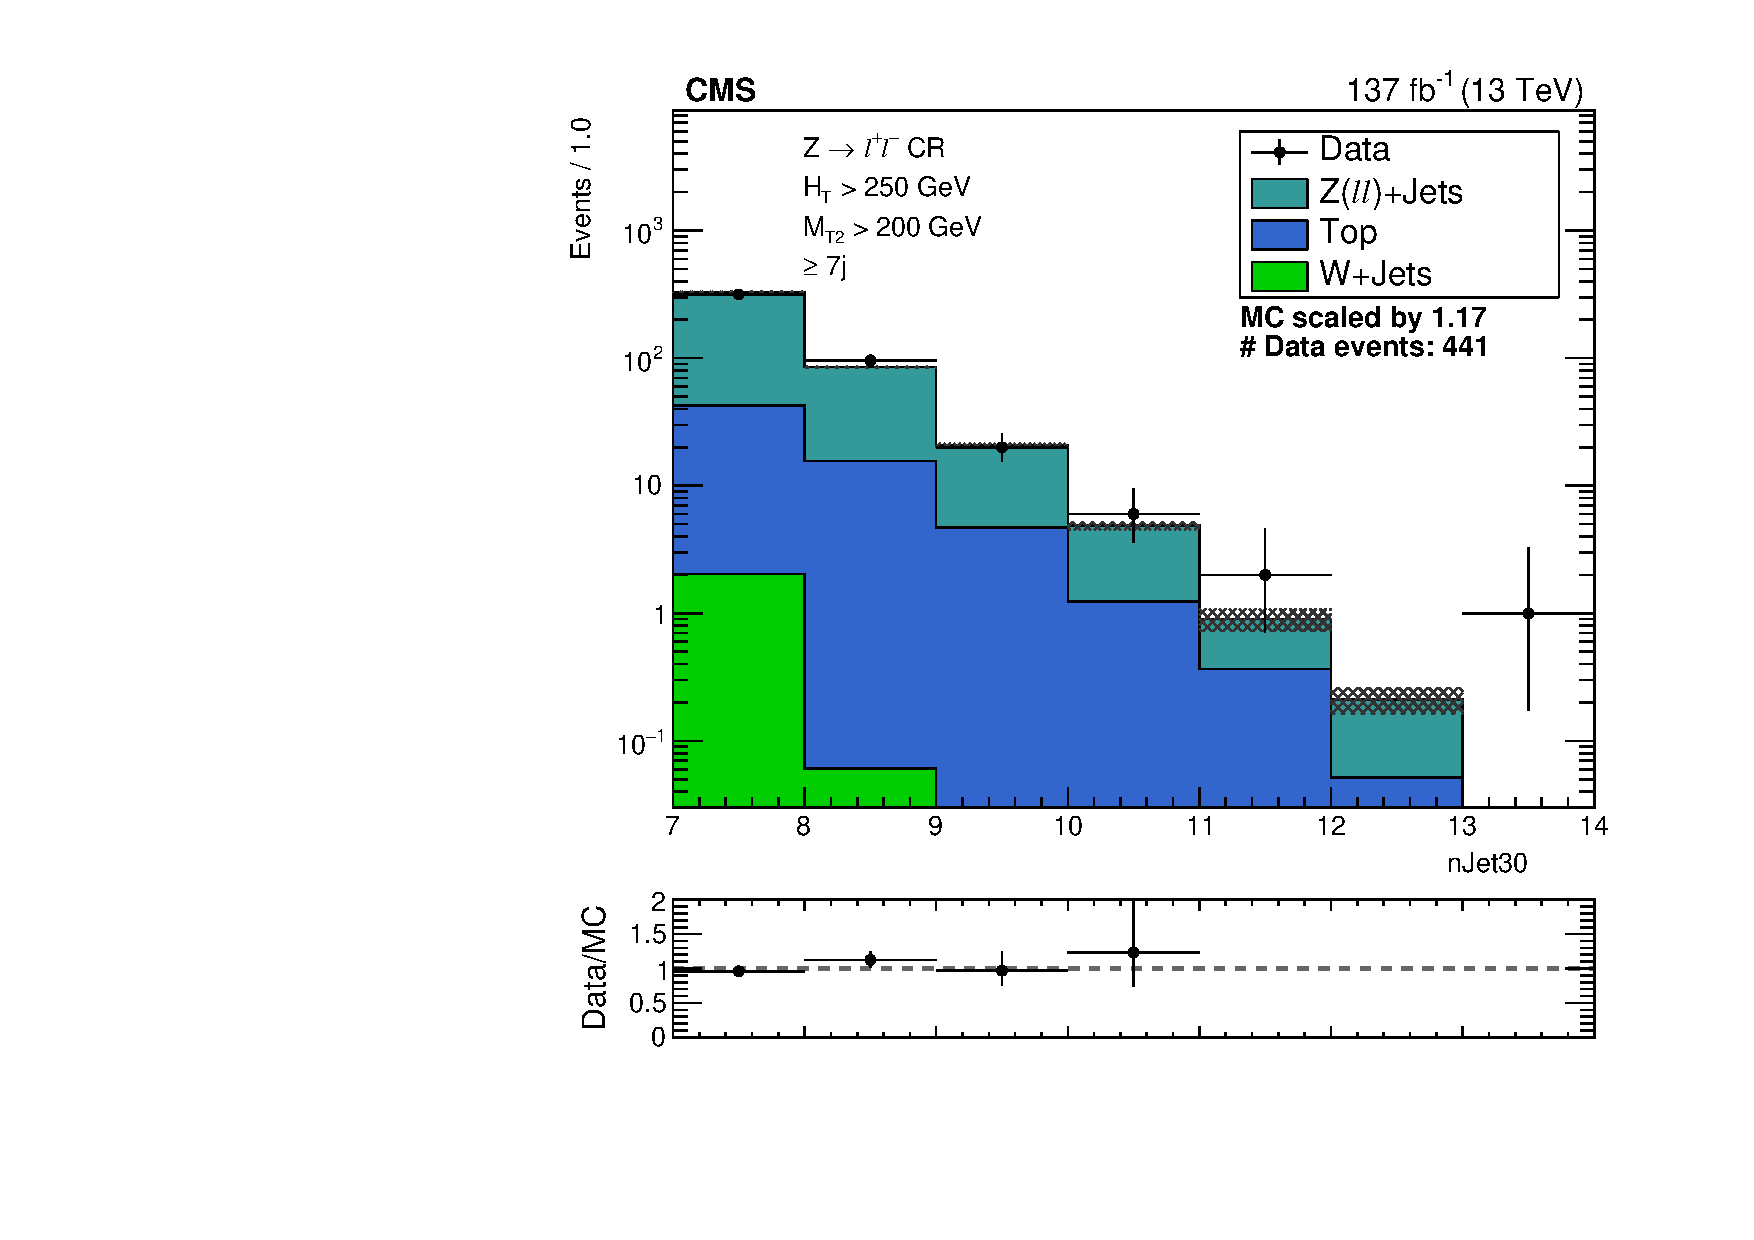
\includegraphics[width=0.48\textwidth]{figs/zinv/crdybase_nJet30_ge7j.pdf}
    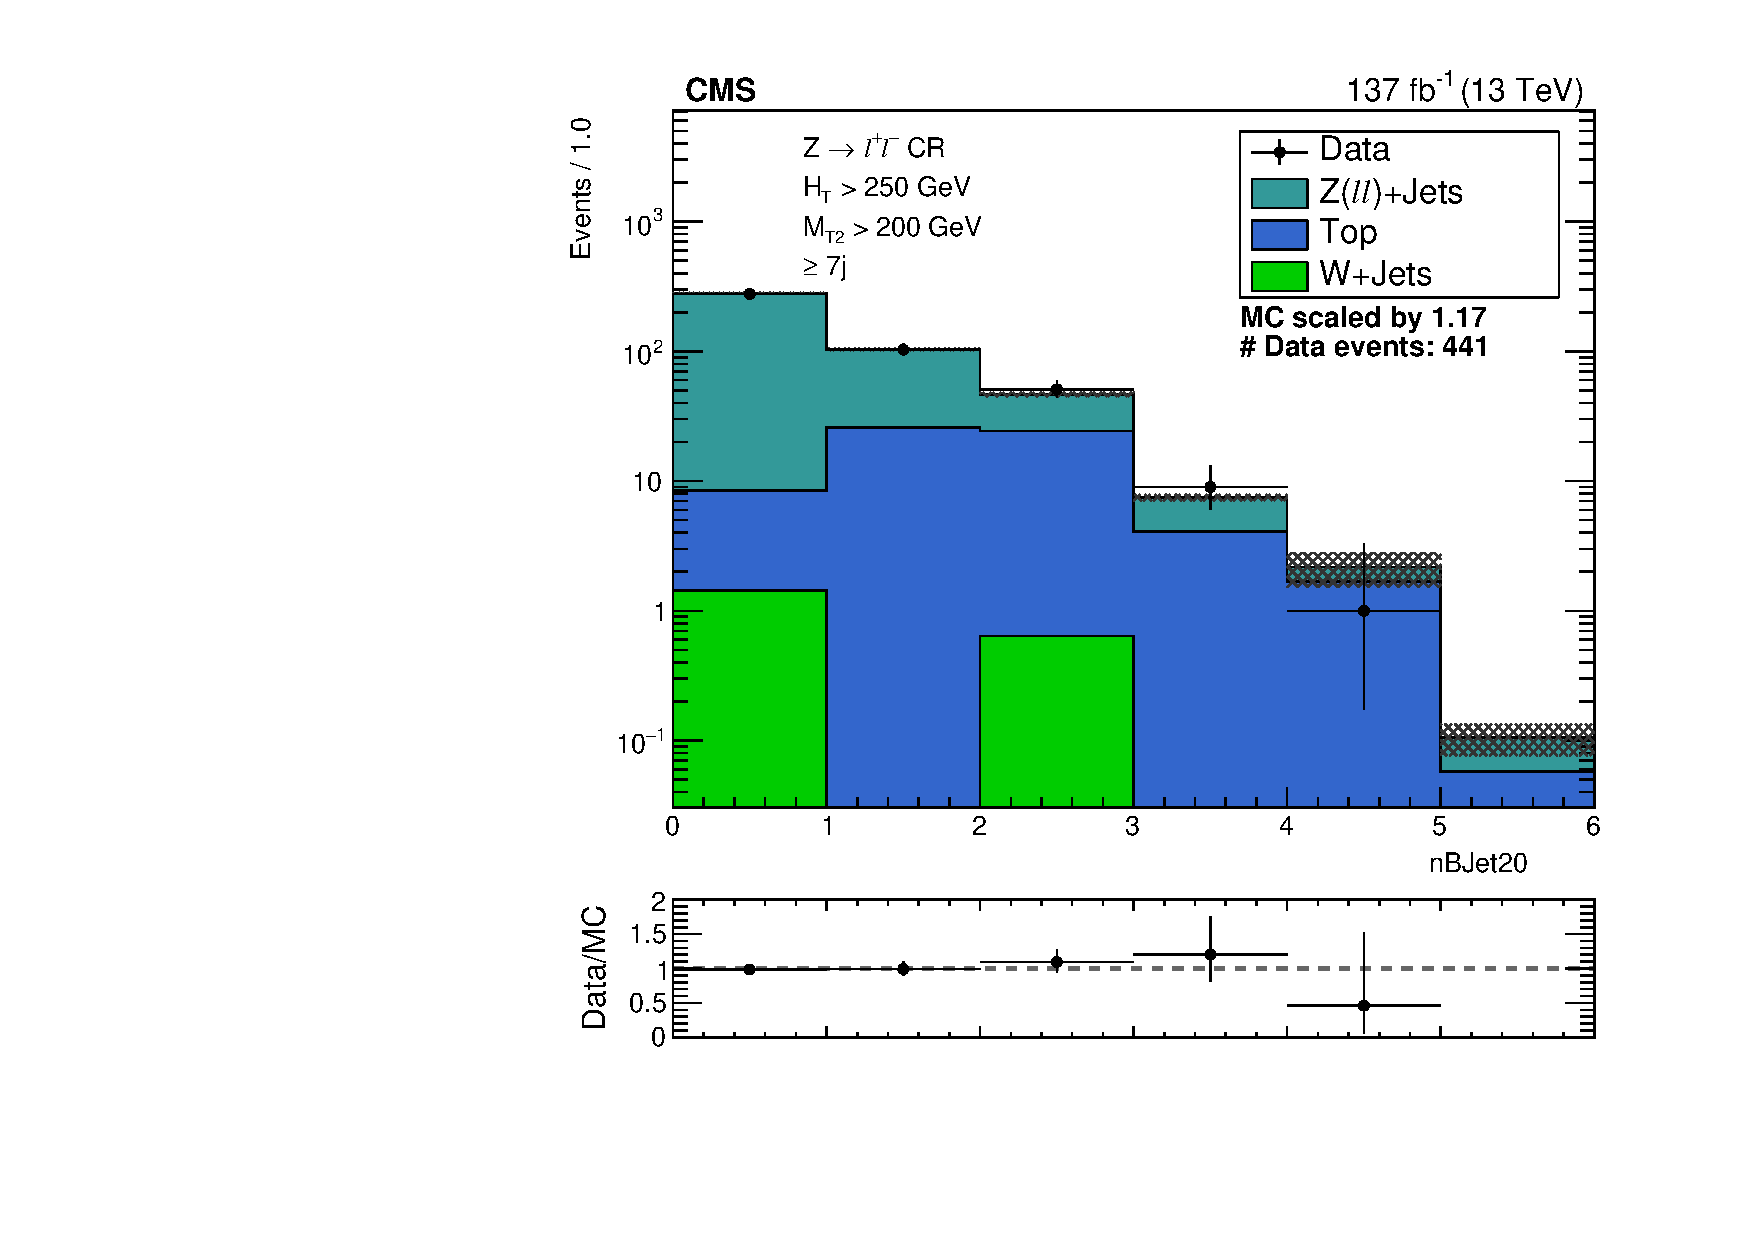
\includegraphics[width=0.48\textwidth]{figs/zinv/crdybase_nBJet20_ge7j.pdf} \\
    \caption{Comparisons of \Nj and \Nb in the $\Nj\geq7$ region. In these high-\Nj regions, 
      shapes of \Nj and \Nb are taken directly from MC as statistics in data are insufficient.
      Monte Carlo is seen to agree well with the observed data in the control region, 
      validating its use to predict signal region yields.
            }
    \label{fig:zll_ge7j}
  \end{center}
\end{figure}


The final estimate in each $(\Ht,\Nj,\Nb,\mttwo)$ signal region can then be summarized as
\be\label{eq:zinv_est}
N_{\znunu}^\mrm{SR} = \left[ N_\mrm{2-lep}^\mrm{CRSF}\; P_{\zll}\; R_\mrm{MC}^{\znunu/\zll} \right]
(\Omega) \times k_\mrm{hybrid}(\mttwo|\Omega),
\ee
where
\begin{itemize}\setlength\itemsep{0mm}
\item $N_\mrm{2-lep}^\mrm{CRSF}$, $P_{\zll}$, and $R_\mrm{MC}^{\znunu/\zll}$ are measured in each topological
region (referred to here as $\Omega\equiv(\Ht,\Nj,\Nb)$), integrated over \mttwo.
\item $N_\mrm{2-lep}^\mrm{CRSF}$ is the number of observed events in data in the same-flavor dilepton control region.
\item $P_{\zll}$ is the \emph{purity}, or fraction of \zll events in the dilepton control region
(see Sec.~\ref{sec:dilep_bkgs}).
\item $R_\mrm{MC}^{\znunu/\zll}$ is the ratio between \znunu and \zll MC yields in this region.
\item $k_\mrm{hybrid}(\mttwo|\Omega)$ is a normalized template used to distribute events as a function
of \mttwo in each topological region (see Sec.~\ref{sec:zinv_mt2}).
\end{itemize}

The values of $N_\mrm{2-lep}^\mrm{CRSF}$, $P_{\zll}$, and $R_\mrm{MC}^{\znunu/\zll}$ for each topological 
region are given in Tables~\ref{tab:estimateZinv_lowHt} and \ref{tab:estimateZinv_highHt}.

\subsection{\zll purity in the dilepton control region}
\label{sec:dilep_bkgs}
While \zll is the process of interest in the dilepton control region, other SM processes can
produce similar same-flavor dilepton signatures. Most prominent is \ttbar production, but other
processes contribute in more minor ways, such as $t\bar{t}V$, diboson, and \wjets (with a fake
lepton) production.

Certain kinematic cuts placed in the dilepton control region ensure that the contributions
from these other processes are as small as possible. The $|m_{\ell\ell}-m_Z|<20\GeV$ cut requires
that the dilepton mass is consistent with $Z$ boson decay. Furthermore, the $\pt(\ell\ell)>200\GeV$ cut
selects events in which the leptons are the primary source of \ptmiss in the event (once their \vSS{p}{T}{}
vectors are added to the \vMet). When this is the case, the $\ptmiss>250\GeV$ cut means that
$\pt(\ell\ell)$ must be large. If, however, there are contributions to the \ptmiss from actual
invisible particles (such as the neutrinos present in all of the secondary production modes listed above),
$\pt(\ell\ell)$ is generally smaller. This is illustrated in Fig.~\ref{fig:zllpt}, which shows a distribution
of $\pt(\ell\ell)$ in the baseline dilepton control region (with the $m_{\ell\ell}$ cut inverted for
$\pt(\ell\ell)<200\GeV$). We see that the $\pt(\ell\ell)>200\GeV$ region is almost entirely from \zll events,
and the $\pt(\ell\ell)<200\GeV$ region comes predominantly from top (\ttbar and $t\bar{t}V$) processes.

\begin{figure}[ht]
  \begin{center}
    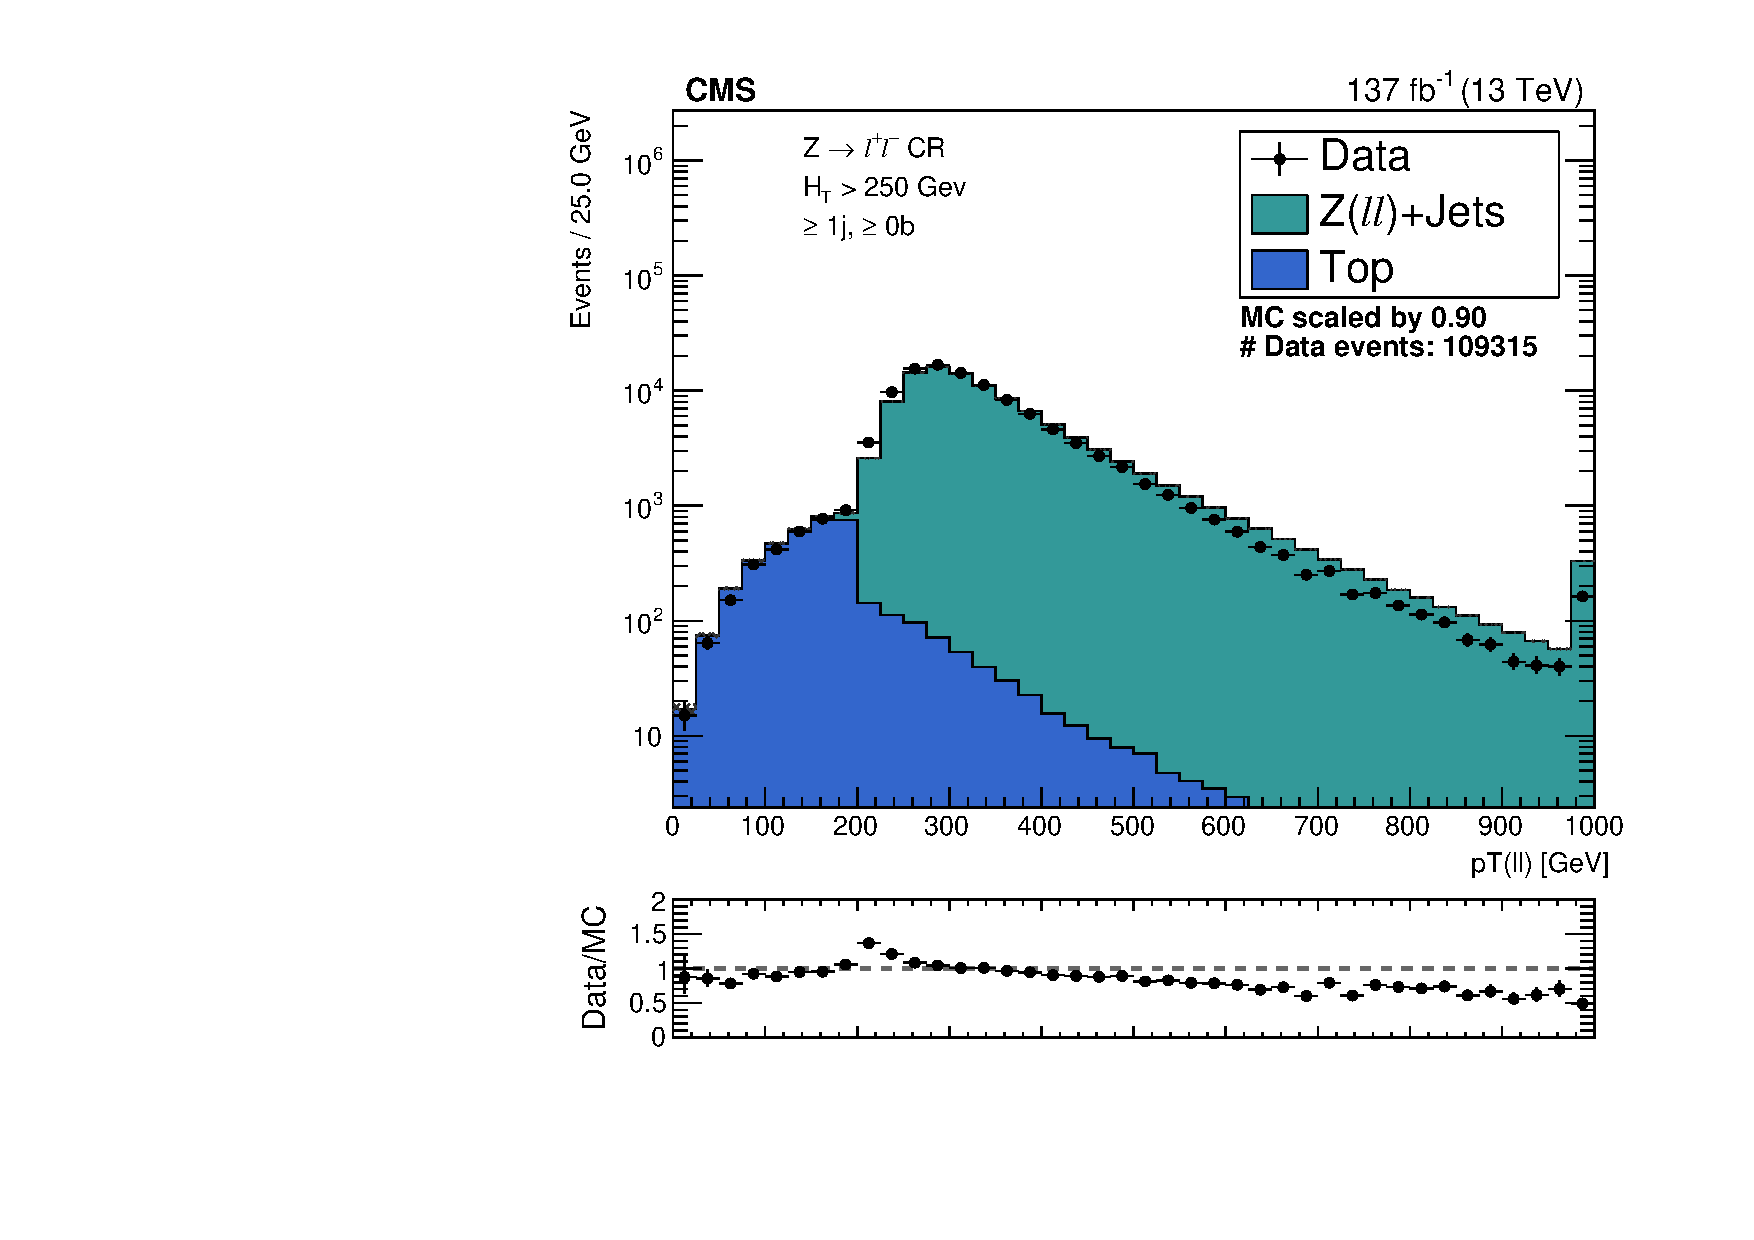
\includegraphics[width=0.55\textwidth]{figs/zinv/crdybase_zllpt.pdf}
    \caption{$\pt(\ell\ell)$ in the baseline dilepton control region, with the exception
      of the $|m_{\ell\ell}-m_Z|<20\GeV$ cut which is inverted for the $\pt(\ell\ell)<200\GeV$
      portion of the plot. We see that the $m_{\ell\ell}$ and $\pt(\ell\ell)$ requirements ensure
      that the control region is predominantly from \zll, and inverting these requirements produces
      a region enriched in top processes (used to measure $R^\mrm{SF/OF}$).
            }
    \label{fig:zllpt}
  \end{center}
\end{figure}

Despite the attempts made to purify the control region with \zll events, there is nevertheless some contamination
from non-$Z$ processes. To estimate and subtract off this contamination, we make use of the fact that
all of the secondary processes are flavor-symmetric, in that they produce opposite-flavor ($e\mu$) events
at the same rate as same-flavor ($ee$ or $\mu\mu$) events. Hence, we can measure their rate in an 
opposite-flavor (OF) control region (same cuts as the nominal same-flavor (SF) dilepton control region, but 
requiring one $e$ and one $\mu$), and then convert this to an estimated same-flavor rate by 
multiplying by a transfer factor $R^\mrm{SF/OF}$.

While this SF/OF ratio is in theory equal to 1 at the production level (since branching fractions to electrons
and muons are the same), different reconstruction efficiencies for electrons and muons cause it to deviate 
from 1 at the reconstructed level. We measure this ratio in data in a top-enriched dilepton control region,
which is the same as the baseline dilepton control region but with $|m_{\ell\ell}-m_Z|>20\GeV$ and
$\pt(\ell\ell)<200\GeV$ (the portion of Fig.~\ref{fig:zllpt} with $\pt(\ell\ell)$ below 200\GeV).
The measurement is done inclusively in all analysis variables, to get a single number that is applied 
to every topological region. The measured ratio is plotted as a function of the analysis variables to
ensure that it is actually constant, and a systematic uncertainty on $R^\mrm{SF/OF}$ is assessed to
cover for any observed variation.

\begin{figure}[t]
  \begin{center}
    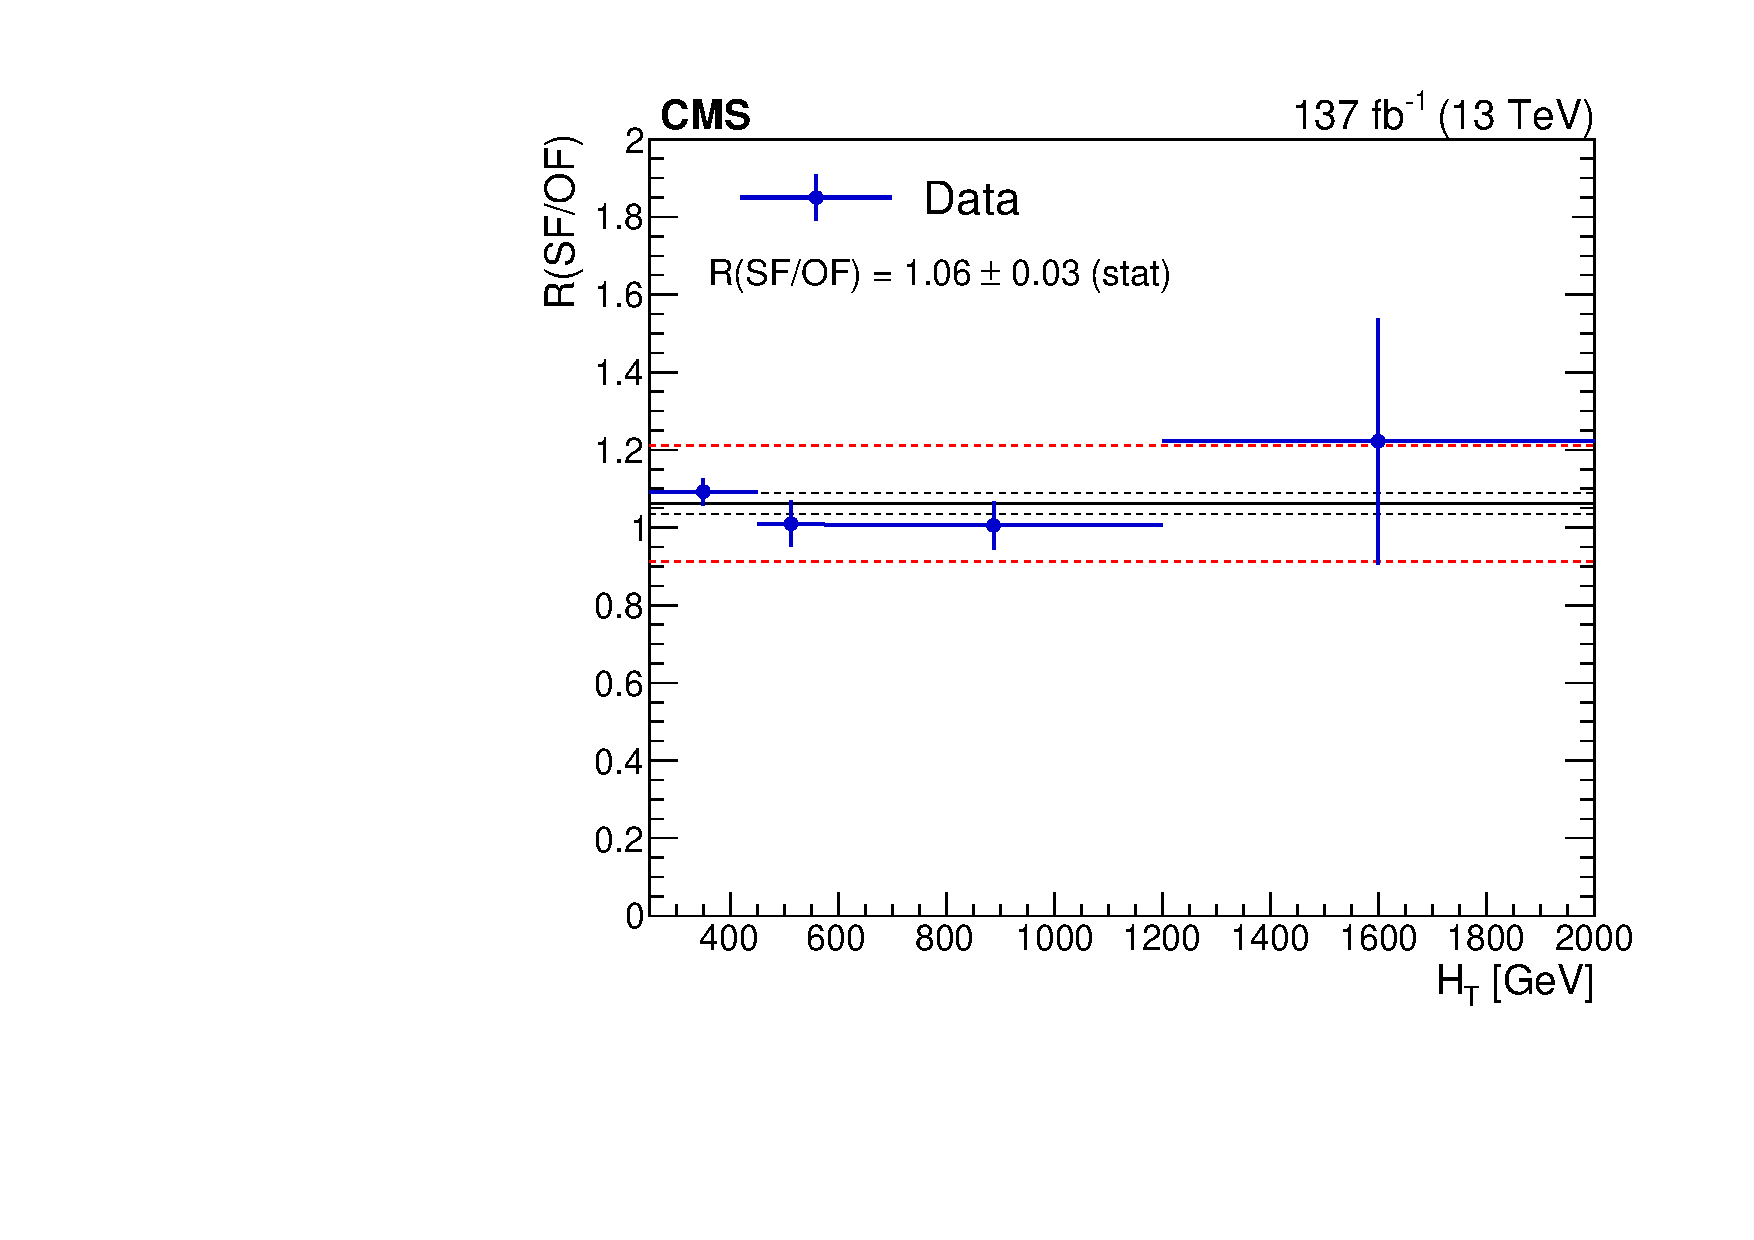
\includegraphics[width=0.48\textwidth]{figs/zinv/rsfof_ht.pdf}
    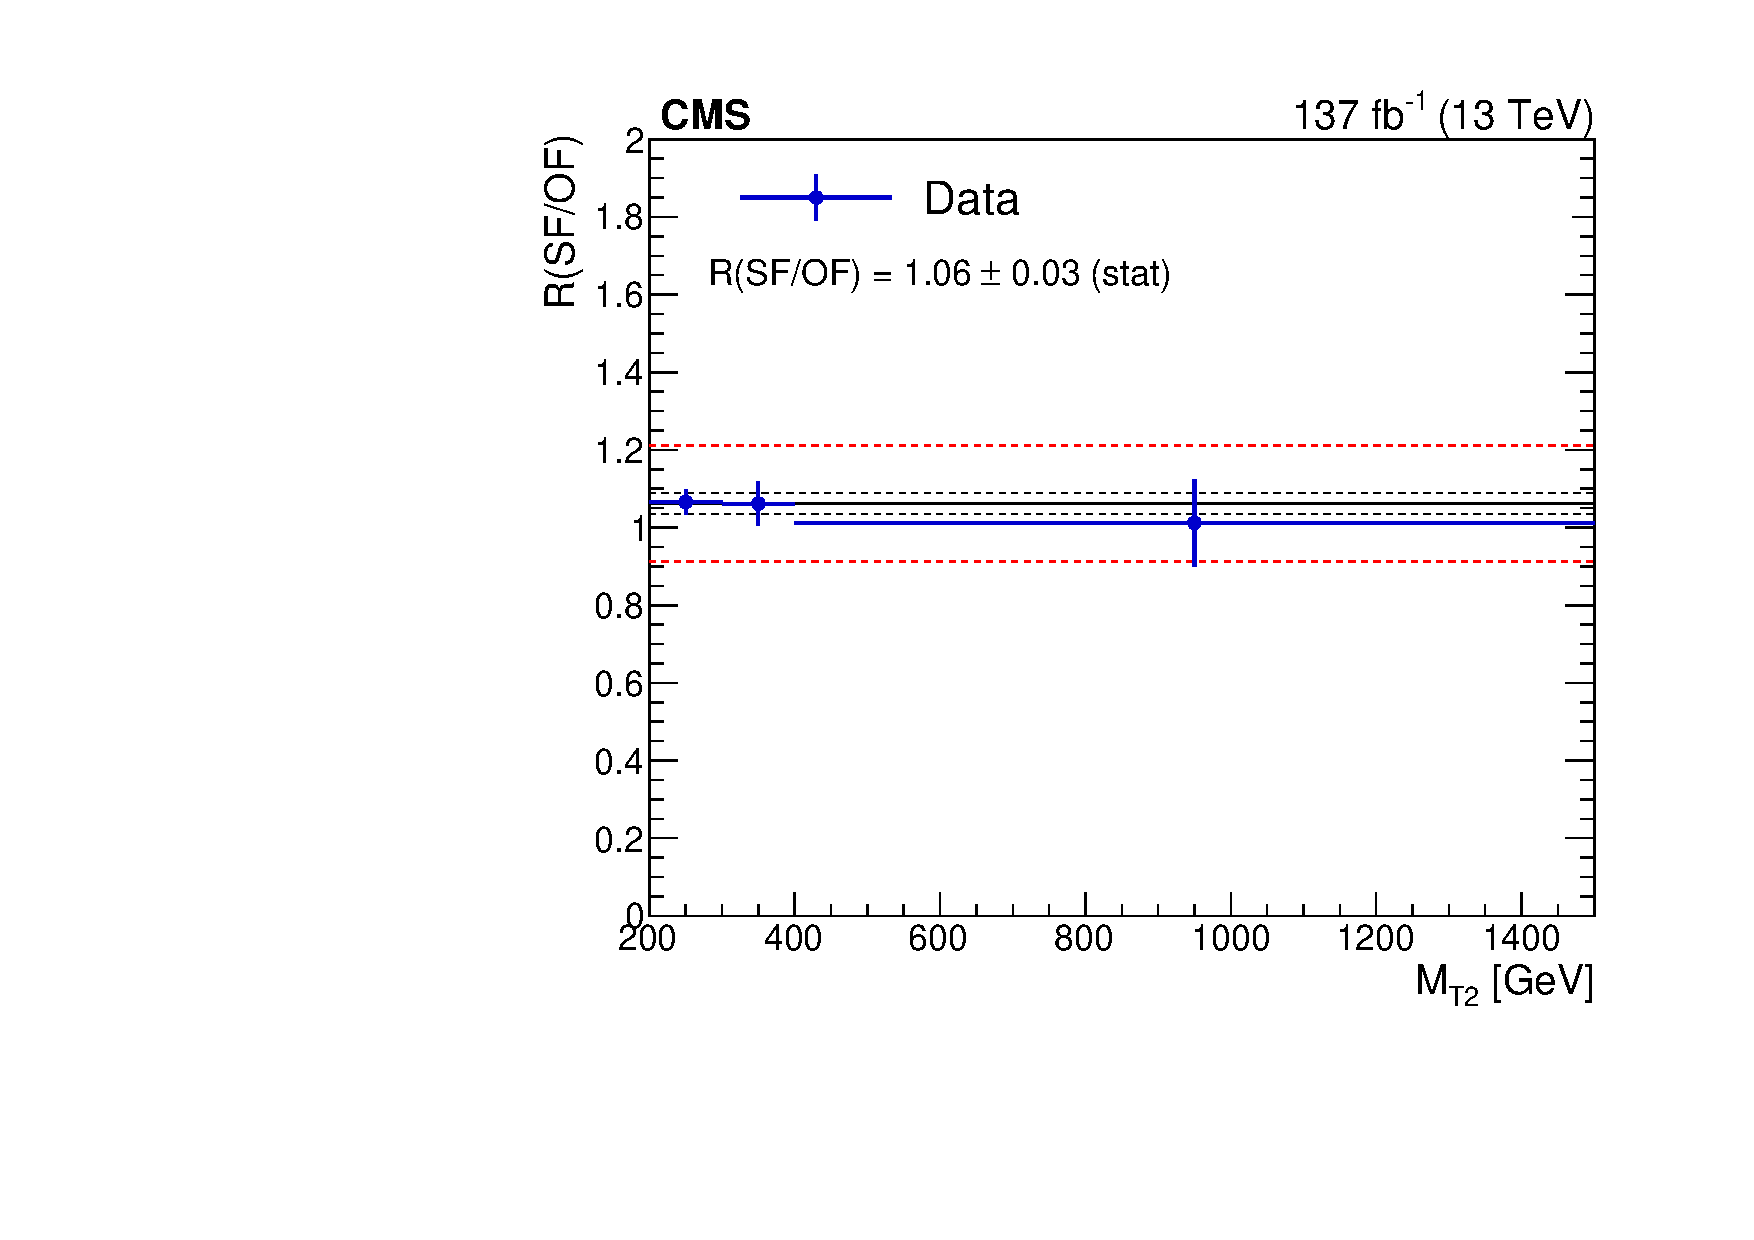
\includegraphics[width=0.48\textwidth]{figs/zinv/rsfof_mt2.pdf} \\
    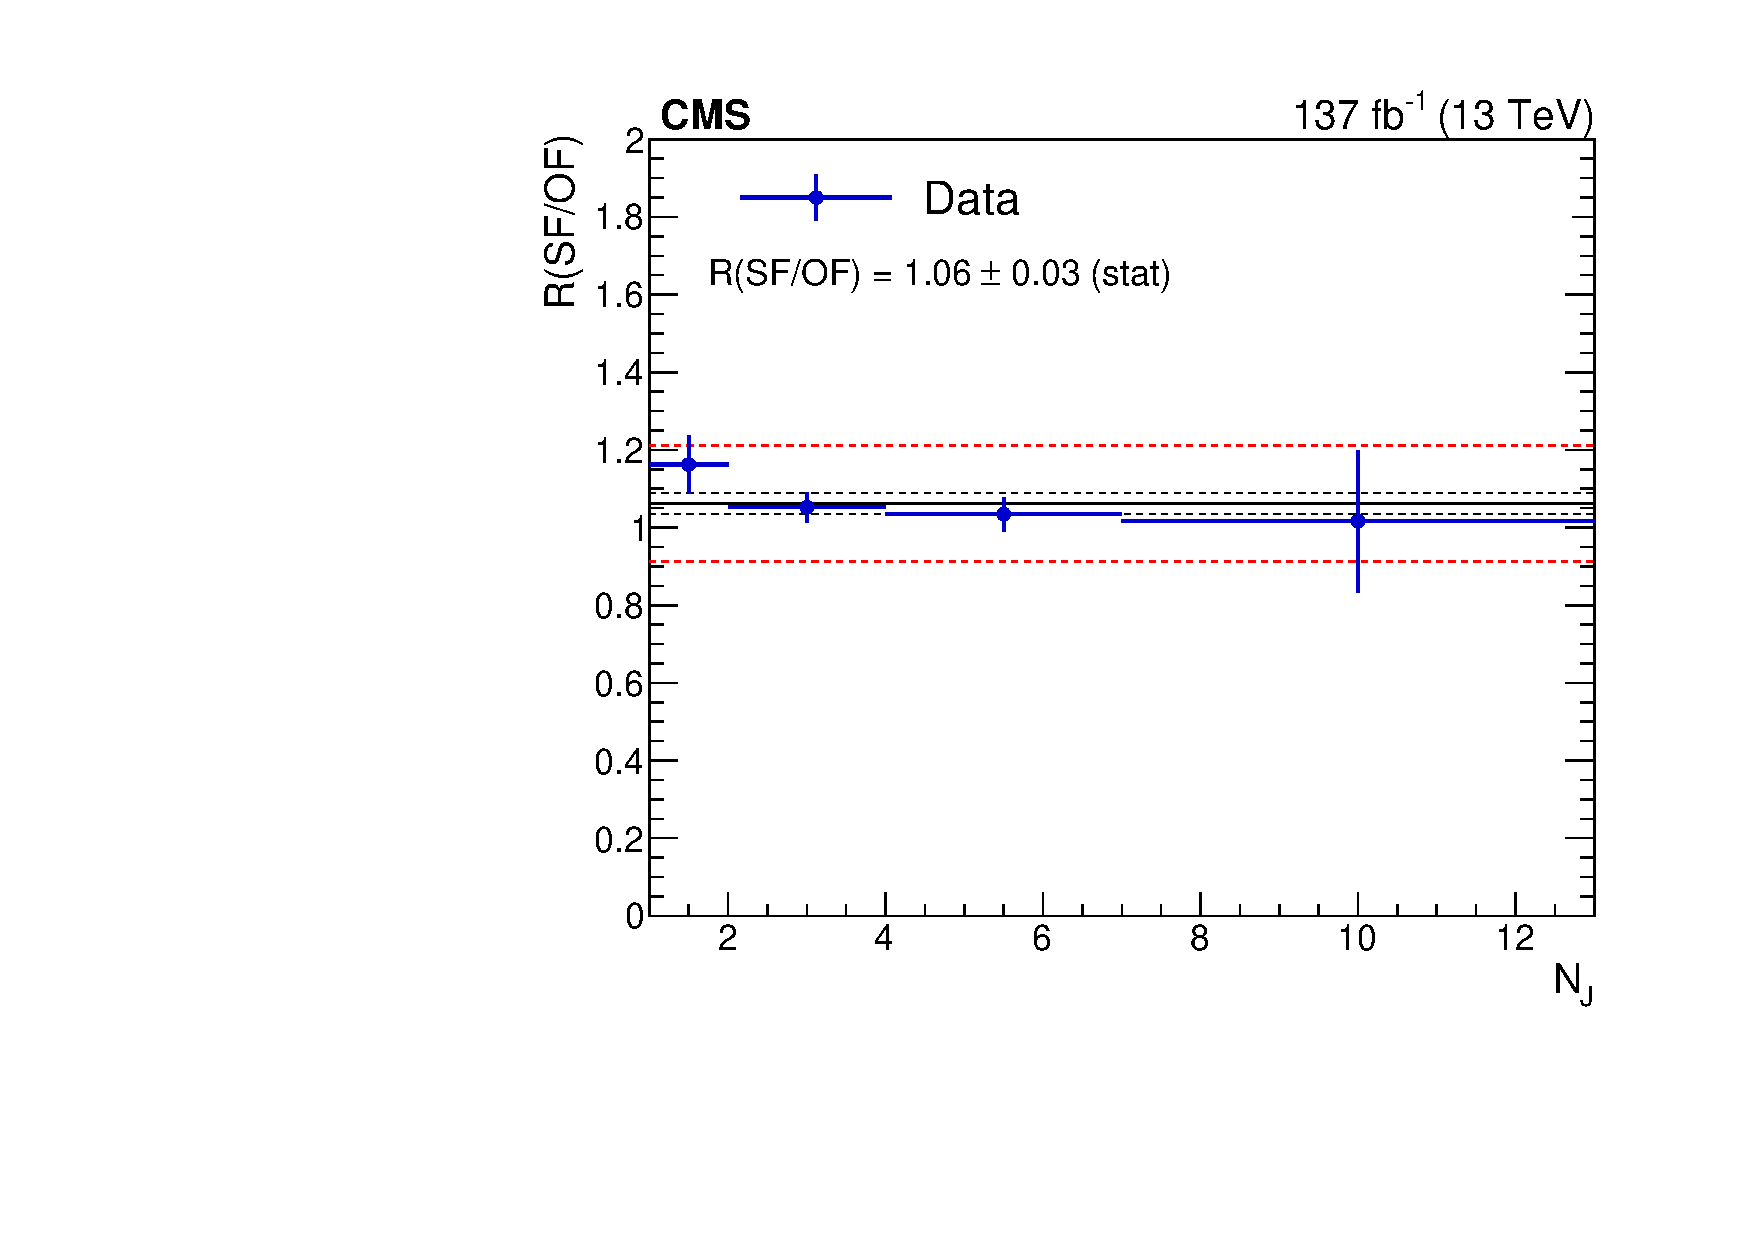
\includegraphics[width=0.48\textwidth]{figs/zinv/rsfof_nJet30.pdf}
    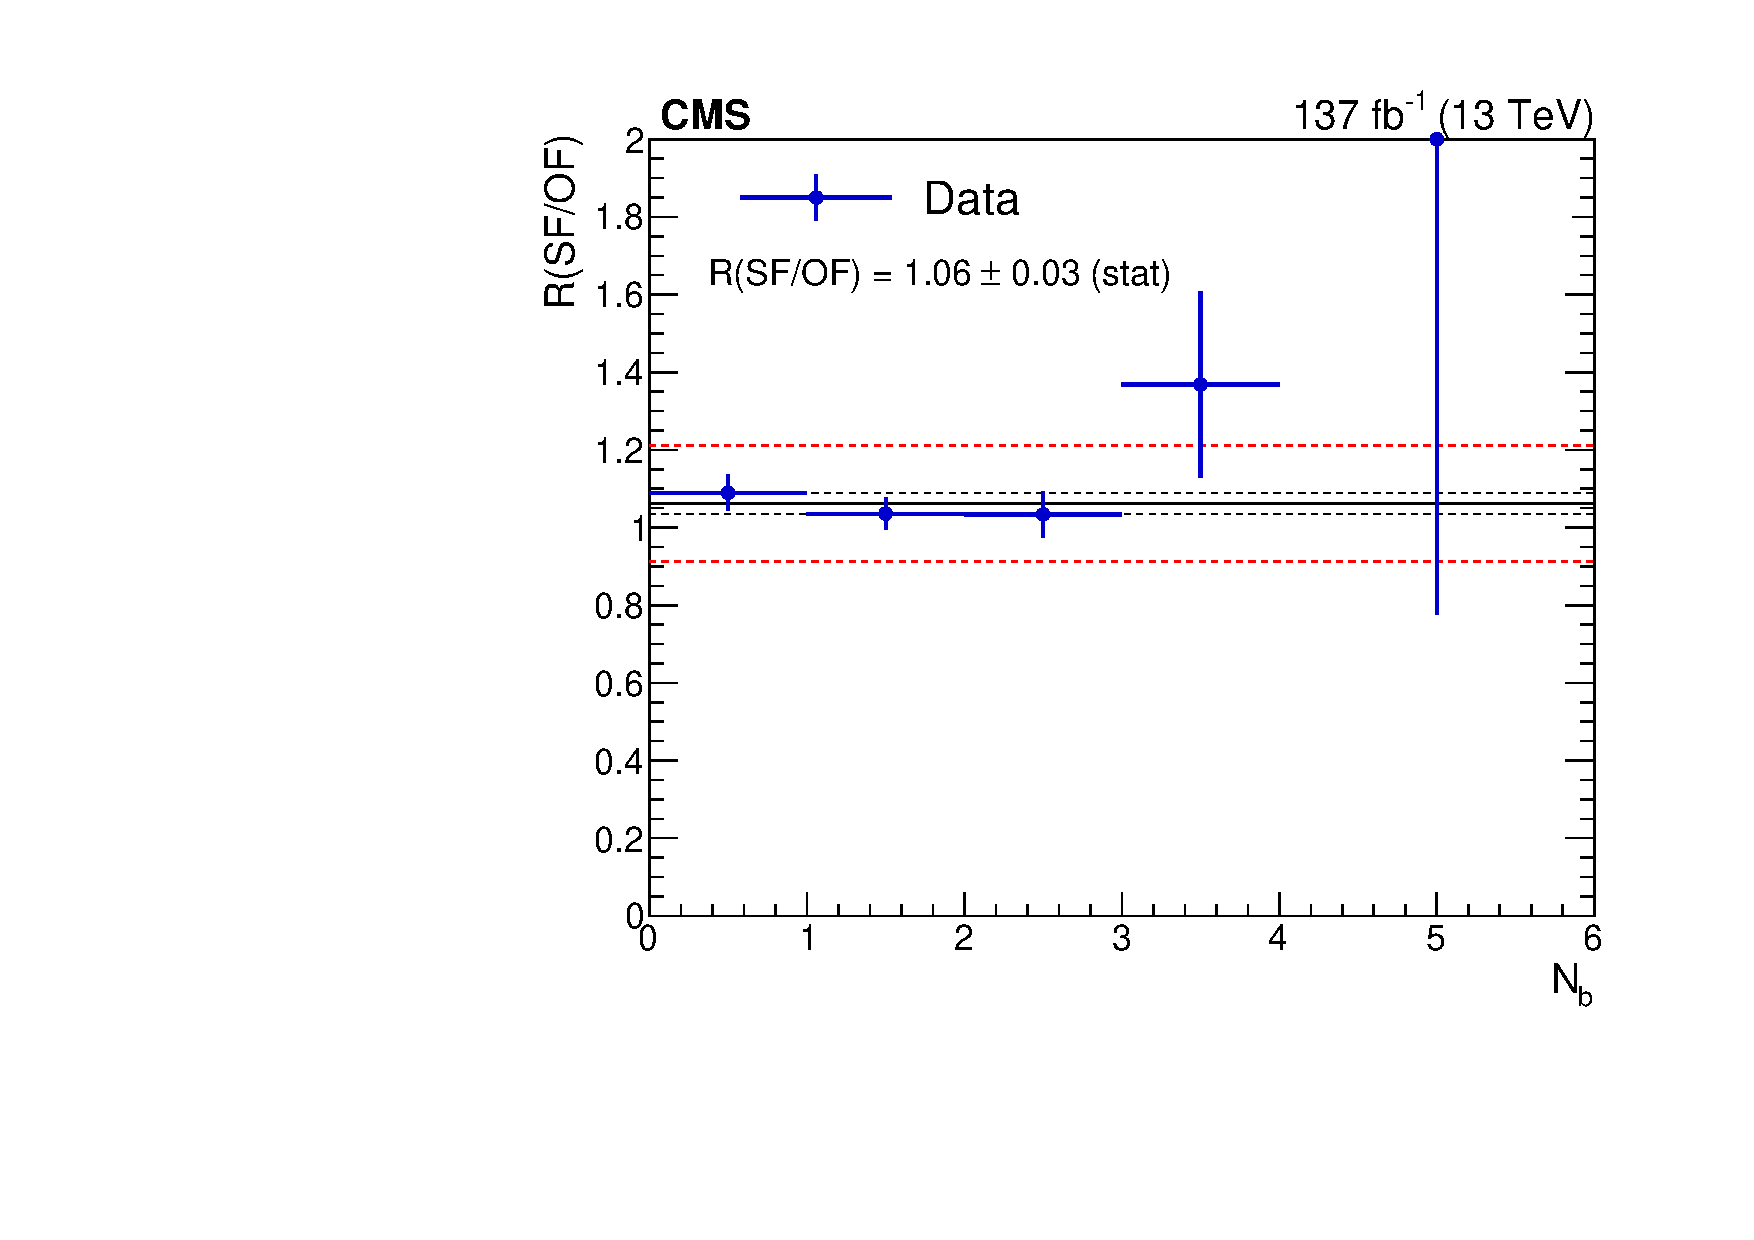
\includegraphics[width=0.48\textwidth]{figs/zinv/rsfof_nBJet20.pdf}
    \caption{Measured $R^\mrm{SF/OF}$ as a function of \Ht, \mttwo, \Nj, and \Nb.
      The black lines show the measured value of $1.06\pm0.03$. The dotted red lines
      show the 15\% systematic uncertainty assessed to cover for any kinematic variation
      in the ratio.
            }
    \label{fig:rsfof}
  \end{center}
\end{figure}

This is illustrated in Fig.~\ref{fig:rsfof}, in which $R^\mrm{SF/OF}$ as measured in data is plotted
as a function of \Ht, \mttwo, \Nj, and \Nb. The ratio is measured to be $1.06\pm0.03$, and is seen to 
be approximately independent of the kinematic variables. To cover for the small observed variation, 
a systematic uncertainty of 0.15 is placed on $R^\mrm{SF/OF}$ and propagated to the final estimate.

Once $R^\mrm{SF/OF}$ is measured, we can compute the purity $P_{\zll}$ used in Eq.~\ref{eq:zinv_est} 
(measured independently in each topological region as) as
\be
P_{\zll} = 1 - R^\mrm{SF/OF} N_\mrm{2-lep}^\mrm{CROF} / N_\mrm{2-lep}^\mrm{CRSF},
\ee
where $N_\mrm{2-lep}^\mrm{CROF}$ is the number of observed events in data in the opposite-flavor
dilepton control region. The values of $N_\mrm{2-lep}^\mrm{CROF}$ and $P_{\zll}$ in each
topological region are given in Tables~\ref{tab:estimateZinv_lowHt} and \ref{tab:estimateZinv_highHt}.

\begin{table}[!ht]
\caption{\label{tab:estimateZinv_lowHt} The control region 
 Drell-Yan (DY) MC yield, same-flavor (SF) and opposite-flavor (OF)
 data yields, purity, and $R^{\znunu/\zll}_{\mrm{MC}}$ for the \znunu
 estimate as a function of \Ht, \Nj, and \Nb, in the monojet, Very Low \Ht, and Low \Ht regions. Note that the the
 regions marked with a * or $^\dagger$  share the same control region (with the same yield and purity),
 and the distribution of events in the  \Nb and/or \Nj dimensions are folded into the  $R^{\znunu/\zll}_{\mrm{MC}}$ value.}
\centering
\resizebox{0.75\textwidth}{!}{%
\renewcommand{\arraystretch}{1.1}
\begin{tabular}{ccc|ccccc}
\hline
\multicolumn{8}{c}{Invisible Z} \\ \hline
\multicolumn{3}{c}{Region} & \multirow{2}{*}{DY yield} & \multirow{2}{*}{SF yield} & \multirow{2}{*}{OF yield} & \multirow{2}{*}{Purity} & \multirow{2}{*}{$R^{\znunu/\zll}_{\mrm{MC}}$} \\
\Ht [GeV] & \Nj & \Nb & & & & & \\
\hline 
$[250,350]$ & 1 & 0 & 30647.5 & 27100 & 6 & $0.998^{+0.001}_{-0.001}$ & $6.15 \pm 0.02$ \\ 
$[350,450]$ & 1 & 0 & 9680.6 & 7891 & 5 & $0.996^{+0.002}_{-0.003}$ & $5.11 \pm 0.02$ \\ 
$[450,575]$ & 1 & 0 & 3414.1 & 2375 & 3 & $0.996^{+0.002}_{-0.004}$ & $4.59 \pm 0.02$ \\ 
$[575,700]$ & 1 & 0 & 985.6 & 610 & 2 & $0.988^{+0.008}_{-0.016}$ & $4.3 \pm 0.02$ \\ 
$[700,1000]$ & 1 & 0 & 480.3 & 265 & 1 & $0.992^{+0.007}_{-0.019}$ & $4.09 \pm 0.03$ \\ 
$[1000,1200]$ & 1 & 0 & 47.5 & 21 & 0 & $1.000^{+0.000}_{-0.094}$ & $4.11 \pm 0.1$ \\ 
${>}1200$ & 1 & 0 & 16.0 & 7 & 0 & $1.000^{+0.000}_{-0.281}$ & $6.53 \pm 0.38$ \\ 
$[250,350]$ & 1 & $\geq1$ & 1771.9 & 1593 & 2 & $0.997^{+0.002}_{-0.004}$ & $5.69 \pm 0.08$ \\ 
$[350,450]$ & 1 & $\geq1$ & 531.3 & 460 & 1 & $0.993^{+0.006}_{-0.016}$ & $4.76 \pm 0.08$ \\ 
$[450,575]$ & 1 & $\geq1$ & 178.6 & 152 & 1 & $0.986^{+0.012}_{-0.032}$ & $4.35 \pm 0.08$ \\ 
$[575,700]$ & 1 & $\geq1$ & 48.0 & 40 & 0 & $1.000^{+0.000}_{-0.049}$ & $4.11 \pm 0.1$ \\ 
${>}700$ & 1 & $\geq1$ & 23.0 & 20 & 1 & $0.947^{+0.044}_{-0.123}$ & $7.38 \pm 1.73$ \\ 
\hline 
$[250,450]$ & 2-3 & 0 & 32020.2 & 31566 & 11 & $0.996^{+0.001}_{-0.002}$ & $6.01 \pm 0.04$ \\ 
$[250,450]$ & 2-3 & 1 & 3461.3 & 4038 & 8 & $0.984^{+0.005}_{-0.008}$ & $5.7 \pm 0.05$ \\ 
$[250,450]$ & 2-3 & 2 & 471.8 & 523 & 3 & $0.980^{+0.011}_{-0.020}$ & $5.54 \pm 0.11$ \\ 
$[250,450]$ & 4-6 & 0 & 3892.5 & 4181 & 5 & $0.996^{+0.002}_{-0.003}$ & $6.35 \pm 0.11$ \\ 
$[250,450]$ & 4-6 & 1 & 662.4 & 875 & 5 & $0.971^{+0.013}_{-0.020}$ & $6.2 \pm 0.13$ \\ 
$[250,450]$ & 4-6 & 2 & 150.5 & 212 & 3 & $0.934^{+0.036}_{-0.064}$ & $5.68 \pm 0.2$ \\ 
$[250,450]$ & $\geq7$ & 0 & 6.5 & 12 & 2 & $0.911^{+0.058}_{-0.118}$ & $6.32 \pm 2.15$ \\ 
$[250,450]$ & $\geq7$ & 1 & 1.6 & 3 & 0 & $1.000^{+0.000}_{-0.657}$ & $7.31 \pm 2.92$ $^{(*)}$ \\ 
$[250,450]$ & $\geq7$ & 2 & 1.6 & 3 & 0 & $1.000^{+0.000}_{-0.657}$ & $2.23 \pm 0.99$ $^{(*)}$ \\ 
$[250,450]$ & 2-6 & $\geq3$ & 23.5 & 36 & 2 & $0.941^{+0.038}_{-0.078}$ & $6.51 \pm 0.5$ \\ 
$[250,450]$ & $\geq7$ & $\geq3$ & 1.6 & 3 & 0 & $1.000^{+0.000}_{-0.657}$ & $0.38 \pm 0.26$ $^{(*)}$ \\ 
\hline 
$[450,575]$ & 2-3 & 0 & 8588.5 & 7288 & 5 & $0.996^{+0.002}_{-0.003}$ & $5.16 \pm 0.06$ \\ 
$[450,575]$ & 2-3 & 1 & 951.2 & 943 & 5 & $0.976^{+0.010}_{-0.016}$ & $5.07 \pm 0.06$ \\ 
$[450,575]$ & 2-3 & 2 & 113.0 & 128 & 3 & $0.941^{+0.032}_{-0.057}$ & $4.97 \pm 0.09$ \\ 
$[450,575]$ & 4-6 & 0 & 2789.8 & 2590 & 5 & $0.993^{+0.003}_{-0.005}$ & $5.7 \pm 0.11$ \\ 
$[450,575]$ & 4-6 & 1 & 499.2 & 599 & 5 & $0.970^{+0.013}_{-0.021}$ & $5.55 \pm 0.11$ \\ 
$[450,575]$ & 4-6 & 2 & 104.3 & 136 & 3 & $0.937^{+0.034}_{-0.061}$ & $5.56 \pm 0.13$ \\ 
$[450,575]$ & $\geq7$ & 0 & 26.2 & 40 & 0 & $1.000^{+0.000}_{-0.049}$ & $6.05 \pm 0.7$ \\ 
$[450,575]$ & $\geq7$ & 1 & 8.5 & 19 & 0 & $1.000^{+0.000}_{-0.104}$ & $5.02 \pm 0.64$ $^{(*)}$ \\ 
$[450,575]$ & $\geq7$ & 2 & 8.5 & 19 & 0 & $1.000^{+0.000}_{-0.104}$ & $1.5 \pm 0.21$ $^{(*)}$ \\ 
$[450,575]$ & 2-6 & $\geq3$ & 12.3 & 18 & 2 & $0.941^{+0.038}_{-0.078}$ & $6.07 \pm 0.29$ \\ 
$[450,575]$ & $\geq7$ & $\geq3$ & 8.5 & 19 & 0 & $1.000^{+0.000}_{-0.104}$ & $0.17 \pm 0.04$ $^{(*)}$ \\ 
\hline
\end{tabular}
}
\end{table}


\begin{table}[!htbp]
\caption{\label{tab:estimateZinv_highHt} Same as Table~\ref{tab:estimateZinv_lowHt}, but for
  the Medium, High, and Extreme \Ht regions }
\centering
\resizebox{0.75\textwidth}{!}{%
\renewcommand{\arraystretch}{1.1}
\begin{tabular}{ccc|ccccc}
\hline
\multicolumn{8}{c}{Invisible Z} \\ \hline
\multicolumn{3}{c}{Region} & \multirow{2}{*}{DY yield} & \multirow{2}{*}{SF yield} & \multirow{2}{*}{OF yield} & \multirow{2}{*}{Purity} & \multirow{2}{*}{$R^{\znunu/\zll}_{\mrm{MC}}$} \\
\Ht [GeV] & \Nj & \Nb & & & & & \\
\hline 
$[575,1200]$ & 2-3 & 0 & 7454.8 & 5509 & 6 & $0.993^{+0.003}_{-0.004}$ & $4.87 \pm 0.06$ \\ 
$[575,1200]$ & 2-3 & 1 & 832.1 & 738 & 5 & $0.965^{+0.015}_{-0.024}$ & $4.79 \pm 0.06$ \\ 
$[575,1200]$ & 2-3 & 2 & 85.2 & 97 & 3 & $0.890^{+0.060}_{-0.107}$ & $4.85 \pm 0.08$ \\ 
$[575,1200]$ & 4-6 & 0 & 4218.6 & 3619 & 5 & $0.993^{+0.003}_{-0.004}$ & $5.32 \pm 0.08$ \\ 
$[575,1200]$ & 4-6 & 1 & 799.8 & 893 & 6 & $0.960^{+0.016}_{-0.024}$ & $5.23 \pm 0.08$ \\ 
$[575,1200]$ & 4-6 & 2 & 159.2 & 200 & 5 & $0.909^{+0.039}_{-0.062}$ & $5.26 \pm 0.09$ \\ 
$[575,1200]$ & 2-6 & $\geq3$ & 17.5 & 34 & 3 & $0.843^{+0.086}_{-0.153}$ & $5.38 \pm 0.14$ \\ 
$[575,1200]$ & 7-9 & 0 & 148.4 & 173 & 2 & $0.994^{+0.004}_{-0.008}$ & $6.03 \pm 0.35$ $^{(*)}$ \\ 
$[575,1200]$ & 7-9 & 1 & 58.0 & 120 & 3 & $0.929^{+0.039}_{-0.069}$ & $4.51 \pm 0.27$ $^{(\dagger)}$ \\ 
$[575,1200]$ & 7-9 & 2 & 58.0 & 120 & 3 & $0.929^{+0.039}_{-0.069}$ & $1.33 \pm 0.08$ $^{(\dagger)}$ \\ 
$[575,1200]$ & 7-9 & 3 & 58.0 & 120 & 3 & $0.929^{+0.039}_{-0.069}$ & $0.18 \pm 0.01$ $^{(\dagger)}$ \\ 
$[575,1200]$ & 7-9 & $\geq4$ & 58.0 & 120 & 3 & $0.929^{+0.039}_{-0.069}$ & $0.033 \pm 0.005$ $^{(\dagger)}$ \\ 
$[575,1200]$ & $\geq10$ & 0 & 148.4 & 173 & 2 & $0.994^{+0.004}_{-0.008}$ & $0.046 \pm 0.015$ $^{(*)}$ \\ 
$[575,1200]$ & $\geq10$ & 1 & 58.0 & 120 & 3 & $0.929^{+0.039}_{-0.069}$ & $0.056 \pm 0.018$ $^{(\dagger)}$ \\ 
$[575,1200]$ & $\geq10$ & 2 & 58.0 & 120 & 3 & $0.929^{+0.039}_{-0.069}$ & $0.017 \pm 0.006$ $^{(\dagger)}$ \\ 
$[575,1200]$ & $\geq10$ & 3 & 58.0 & 120 & 3 & $0.929^{+0.039}_{-0.069}$ & $0.0039 \pm 0.0016$ $^{(\dagger)}$ \\ 
$[575,1200]$ & $\geq10$ & $\geq4$ & 58.0 & 120 & 3 & $0.929^{+0.039}_{-0.069}$ & $0.0 \pm 0.0$ $^{(\dagger)}$ \\ 
\hline 
$[1200,1500]$ & 2-3 & 0 & 300.3 & 194 & 2 & $0.989^{+0.007}_{-0.015}$ & $5.01 \pm 0.34$ \\ 
$[1200,1500]$ & 2-3 & 1 & 33.3 & 24 & 2 & $0.955^{+0.029}_{-0.059}$ & $4.96 \pm 0.35$ \\ 
$[1200,1500]$ & 2-3 & 2 & 2.3 & 3 & 0 & $1.000^{+0.000}_{-0.657}$ & $5.58 \pm 0.59$ \\ 
$[1200,1500]$ & 4-6 & 0 & 288.8 & 236 & 2 & $0.986^{+0.009}_{-0.018}$ & $5.46 \pm 0.32$ \\ 
$[1200,1500]$ & 4-6 & 1 & 59.1 & 73 & 2 & $0.941^{+0.038}_{-0.077}$ & $5.17 \pm 0.31$ \\ 
$[1200,1500]$ & 4-6 & 2 & 10.0 & 11 & 0 & $1.000^{+0.000}_{-0.179}$ & $5.66 \pm 0.4$ \\ 
$[1200,1500]$ & 2-6 & $\geq3$ & 1.3 & 0 & 0 & $1.000^{+0.000}_{-0.000}$ & $4.95 \pm 0.67$ \\ 
$[1200,1500]$ & 7-9 & 0 & 28.1 & 25 & 0 & $1.000^{+0.000}_{-0.079}$ & $5.84 \pm 0.78$ $^{(*)}$ \\ 
$[1200,1500]$ & 7-9 & 1 & 11.5 & 13 & 2 & $0.918^{+0.053}_{-0.109}$ & $4.12 \pm 0.57$ $^{(\dagger)}$ \\ 
$[1200,1500]$ & 7-9 & 2 & 11.5 & 13 & 2 & $0.918^{+0.053}_{-0.109}$ & $1.13 \pm 0.16$ $^{(\dagger)}$ \\ 
$[1200,1500]$ & 7-9 & 3 & 11.5 & 13 & 2 & $0.918^{+0.053}_{-0.109}$ & $0.22 \pm 0.04$ $^{(\dagger)}$ \\ 
$[1200,1500]$ & 7-9 & $\geq4$ & 11.5 & 13 & 2 & $0.918^{+0.053}_{-0.109}$ & $0.03 \pm 0.014$ $^{(\dagger)}$ \\ 
$[1200,1500]$ & $\geq10$ & 0 & 28.1 & 25 & 0 & $1.000^{+0.000}_{-0.079}$ & $0.13 \pm 0.11$ $^{(*)}$ \\ 
$[1200,1500]$ & $\geq10$ & 1 & 11.5 & 13 & 2 & $0.918^{+0.053}_{-0.109}$ & $0.12 \pm 0.1$ $^{(\dagger)}$ \\ 
$[1200,1500]$ & $\geq10$ & 2 & 11.5 & 13 & 2 & $0.918^{+0.053}_{-0.109}$ & $0.047 \pm 0.04$ $^{(\dagger)}$ \\ 
$[1200,1500]$ & $\geq10$ & 3 & 11.5 & 13 & 2 & $0.918^{+0.053}_{-0.109}$ & $0.013 \pm 0.012$ $^{(\dagger)}$ \\ 
$[1200,1500]$ & $\geq10$ & $\geq4$ & 11.5 & 13 & 2 & $0.918^{+0.053}_{-0.109}$ & $0.0085 \pm 0.0106$ $^{(\dagger)}$ \\ 
\hline 
${>}1500$ & 2-3 & 0 & 169.4 & 135 & 0 & $1.000^{+0.000}_{-0.015}$ & $5.24 \pm 0.28$ \\ 
${>}1500$ & 2-3 & 1 & 17.8 & 13 & 0 & $1.000^{+0.000}_{-0.152}$ & $4.87 \pm 0.29$ \\ 
${>}1500$ & 2-3 & 2 & 1.2 & 0 & 0 & $1.000^{+0.000}_{-0.000}$ & $5.11 \pm 0.66$ \\ 
${>}1500$ & 4-6 & 0 & 184.9 & 153 & 2 & $0.993^{+0.005}_{-0.009}$ & $5.49 \pm 0.29$ \\ 
${>}1500$ & 4-6 & 1 & 35.7 & 31 & 2 & $0.896^{+0.067}_{-0.137}$ & $5.52 \pm 0.31$ \\ 
${>}1500$ & 4-6 & 2 & 5.9 & 5 & 2 & $0.786^{+0.138}_{-0.282}$ & $5.17 \pm 0.38$ \\ 
${>}1500$ & 2-6 & $\geq3$ & 0.7 & 1 & 0 & $1.000^{+0.000}_{-1.970}$ & $4.93 \pm 0.81$ \\ 
${>}1500$ & 7-9 & 0 & 22.8 & 27 & 0 & $1.000^{+0.000}_{-0.073}$ & $5.59 \pm 0.32$ $^{(*)}$ \\ 
${>}1500$ & 7-9 & 1 & 9.1 & 9 & 0 & $1.000^{+0.000}_{-0.219}$ & $4.78 \pm 0.32$ $^{(\dagger)}$ \\ 
${>}1500$ & 7-9 & 2 & 9.1 & 9 & 0 & $1.000^{+0.000}_{-0.219}$ & $1.24 \pm 0.1$ $^{(\dagger)}$ \\ 
${>}1500$ & 7-9 & 3 & 9.1 & 9 & 0 & $1.000^{+0.000}_{-0.219}$ & $0.14 \pm 0.02$ $^{(\dagger)}$ \\ 
${>}1500$ & 7-9 & $\geq4$ & 9.1 & 9 & 0 & $1.000^{+0.000}_{-0.219}$ & $0.024 \pm 0.009$ $^{(\dagger)}$ \\ 
${>}1500$ & $\geq10$ & 0 & 22.8 & 27 & 0 & $1.000^{+0.000}_{-0.073}$ & $0.22 \pm 0.02$ $^{(*)}$ \\ 
${>}1500$ & $\geq10$ & 1 & 9.1 & 9 & 0 & $1.000^{+0.000}_{-0.219}$ & $0.24 \pm 0.03$ $^{(\dagger)}$ \\ 
${>}1500$ & $\geq10$ & 2 & 9.1 & 9 & 0 & $1.000^{+0.000}_{-0.219}$ & $0.1 \pm 0.02$ $^{(\dagger)}$ \\ 
${>}1500$ & $\geq10$ & 3 & 9.1 & 9 & 0 & $1.000^{+0.000}_{-0.219}$ & $0.00032 \pm 0.00012$ $^{(\dagger)}$ \\ 
${>}1500$ & $\geq10$ & $\geq4$ & 9.1 & 9 & 0 & $1.000^{+0.000}_{-0.219}$ & $0.0014 \pm 0.001$ $^{(\dagger)}$ \\ 
\hline
\end{tabular}
}
\end{table}



\section{\texorpdfstring{\mttwo}{MT2} extrapolation}
\label{sec:zinv_mt2}

To project the per-topological region estimate described in the previous section along the \mttwo dimension, we use
a ``hybrid'' \mttwo template derived using both data and MC ($k_\mrm{hybrid}(\mttwo|\Omega)$ in Eq.~\ref{eq:zinv_est}).

In every \Ht region, the \mttwo shape for both \znunu and \zll MC events is observed to be independent of \Nb.
An example of this is shown in Fig.~\ref{fig:zinv_nbshape}, for the Medium \Ht region. Furthermore,
in the Extreme \Ht region ($[1500,\infty]\GeV$), the \mttwo shape is observed to also be independent of \Nj
up to \mttwo values of about 1\TeV.

Thus, we build \mttwo shape templates from data and MC in each $(\Ht,\Nj)$ bin for regions
with $\Ht<1500\GeV$, integrating over \Nb, while one single hybrid template is built for the
Extreme $\Ht>1500\GeV$ region, integrating also over \Nj. The one exception is for regions with
exactly 2 or 2--6 jets and $\geq$3 b tags. To avoid sculpting the \Nj distribution by requiring
$\Nb\geq3$, we use regions with $\Nj\geq3$ to obtain \mttwo shape templates in these regions.

\begin{figure}[ht]
  \begin{center}
    \includegraphics[width=0.24\textwidth]{figs/zinv/MT2vsNB_1M.pdf}
    \includegraphics[width=0.24\textwidth]{figs/zinv/MT2vsNB_4M.pdf}
    \includegraphics[width=0.24\textwidth]{figs/zinv/MT2vsNB_7M.pdf}
    \includegraphics[width=0.24\textwidth]{figs/zinv/MT2vsNB_26M.pdf} \\
    \includegraphics[width=0.24\textwidth]{figs/zinv/MT2vsNB_1MDY.pdf}
    \includegraphics[width=0.24\textwidth]{figs/zinv/MT2vsNB_4MDY.pdf}
    \includegraphics[width=0.24\textwidth]{figs/zinv/MT2vsNB_7MDY.pdf}
    \includegraphics[width=0.24\textwidth]{figs/zinv/MT2vsNB_26MDY.pdf} \\
    \caption{Example \mttwo distributions in various bins of \Nj and \Nb in the
      \Ht region $[575,1000]\GeV$, for \zll (top) and \znunu (bottom) MC.
      We see that the \mttwo shape is independent of \Nb in all \Nj regions.
            }
    \label{fig:zinv_nbshape}
  \end{center}
\end{figure}

Starting from the highest \mttwo bin in each topological region in the dilepton control region,
we merge bins until the sum of expected yields in the merged bins is at least 50 events, 
as predicted by MC for the full integrated luminosity of \Lint.
For the lower non-merged \mttwo bins, which have larger statistics, the \mttwo shapes are built
directly from \zll data, corrected by the \znunu/\zll MC ratio in order to account
for lepton reconstruction effects. The \znunu MC \mttwo shape is instead used to distribute
events across the merged \mttwo bins, after renormalizing the MC to the total data yield in
the same bins. For the $\Ht>1500\GeV$ region, we use \Nj-binned \znunu MC shapes for 
the extrapolation, to avoid the mild \Nj dependence observed at high \mttwo.

For the lower \mttwo bins, where the \mttwo shapes are built directly from \zll data, an
uncertainty corresponding to the statistical uncertainty in data in each \mttwo bin is accounted for.
For the bins where \znunu MC is used, an additional systematic uncertainty, as large as 40\%
in the last \mttwo bin, is assessed, as described in Sec.~\ref{sec:zinv_syst}.

This \mttwo shape procedure is validated by comparing \mttwo shapes of
\znunu MC and \zll data from the dilepton control region. Examples of this
for the Low and High \Ht regions are shown in Fig.~\ref{fig:zinv_mt2shape}.
\mttwo shape obtained from dilepton data is shown in red markers, and that
from \znunu MC is shown in black. The grey band corresponds to the systematic
uncertainty assigned to the \znunu shape, as described in Sec.~\ref{sec:zinv_syst}.
It is seen than any discrepancies in shape are covered by the assigned systematic.


\begin{figure}[ht]
  \begin{center}
    \includegraphics[width=0.45\textwidth]{figs/zinv/MT2L_W_GJ_log.pdf}
    \includegraphics[width=0.45\textwidth]{figs/zinv/MT2H_W_GJ_log.pdf}
    \caption{Comparisons of \mttwo shape from \znunu MC (black) and \zll
      data from the dilepton control region (red), for the Low (left) and
      High (right) \Ht regions. The grey band in the ratio plot corresponds
      to the systematic assigned to the \znunu shape, as described in Sec.~\ref{sec:zinv_syst}.
            }
    \label{fig:zinv_mt2shape}
  \end{center}
\end{figure}


\section{Systematic uncertainties}
\label{sec:zinv_syst}

The following systematics are assessed on the \znunu background prediction:
\begin{itemize}\setlength\itemsep{0mm}
\item Control region statistical error: the Poisson error on the observed data count in each \zll control region.
This is correlated among all bins that share a common control region (including the \mttwo bins that utilize a merged control region),
but is otherwise uncorrelated.
\item $R_\mrm{MC}^{\znunu/\zll}$ (stat): from MC statistical uncertainty
\item $R_\mrm{MC}^{\znunu/\zll}$ (syst): $\mathcal{O}$(5-10\%) uncertainty, mainly from lepton efficiency
uncertainties in the dilepton control region. Jet energy scale uncertainties also contribute.
\item Purity (stat): from the 3\% statistical uncertainty on $R^\mrm{SF/OF}$
\item Purity (syst): from the assigned 15\% systematic uncertainty on $R^\mrm{SF/OF}$ to cover
for any kinematic variation
\item \mttwo shape uncertainty: For the data-driven component of the hybrid templates (low-\mttwo,
  high stats bins), this is covered by the CR statistical error listed above. For the MC-driven
  component (higher \mttwo), this is an extra assigned uncertainty based on MC variations in 
  the \mttwo shape, accounting for theoretical (renormalization and factorization scales, parton
  distribution functions) and experimental (jet energy scale, \ptmiss modeling) effects. These
  effects give at most a 20\% variation in the last \mttwo bin in each topological region when
  these parameters are varied in MC. The uncertainty in the last bin is increased to 40\% to
  account for possible mis-modeling of \mttwo in MC. The uncertainty is implemented as a correlated
  linear morphing of the \mttwo shape in the higher \mttwo bins, with a maximum amplitude of 40\% in the last bin, 
  done in such a way as to preserve normalization and only affect the shape. These shape uncertainties
  are not correlated between topological regions.
\end{itemize}

\chapter{Lost Lepton Background}
\label{chap:lostlep}

A second source of background comes from events where a genuine prompt lepton is produced
from the decay of a $W$ boson. While the tight lepton veto employed in the analysis 
aims to eliminate as many of these events as possible, a significant number still enter
the signal regions because the lepton gets ``lost''. This can happen for a number
of reasons, such as the lepton being outside of the acceptance window (i.e. it is too forward
 or the \pt is too small) or not being isolated, or the reconstruction algorithms
failing to identify the candidate as a lepton. 

Generally the energy of the lepton is still
accounted for (making ``lost'' a bit of a misnomer), so there is no fake \ptmiss from the lepton. 
However, there is real \ptmiss from the neutrino from the $W$ decay, and this is often enough
to allow the event to enter the signal region. The dominant production mechanisms for the lost
lepton background are \wjets and \ttbar production, but there are also smaller contributions
from rarer processes such as single top, $\ttbar W$, $\ttbar Z$, $\ttbar H$, and $tt\bar{t}\bar{t}$.

The lost lepton background is estimated in a data-driven way using a control sample of events
where there \emph{is} a reconstructed lepton. Section~\ref{sec:llep_pred} describes how this
is done in each $(\Ht, \Nj, \Nb)$ topological region, Sec.~\ref{sec:llep_mt2} explains the method
for extrapolating along the \mttwo dimension, and Sec.~\ref{sec:llep_syst} lists the systematic
uncertainties assessed on the final estimate.

\section{Prediction from single lepton control regions}
\label{sec:llep_pred}

The lost lepton estimate is performed with single lepton control region, described in detail 
in Sec.~\ref{sec:crsl}. It mainly inverts the  lepton veto employed in the signal regions,
but with the additional requirement that $M_\mrm{T}(\mrm{cand},\vMet)<100\GeV$, in order
to reduce signal contamination. All individual processes (\wjets, \ttbar, etc.) are summed
for the purposes of computing the estimate (i.e. there is only a single transfer factor for all
processes combined).

Data vs. MC comparisons of the main analysis kinematic variables in the baseline single lepton
control region are shown in Fig.~\ref{fig:llep_crplots}. In these plots and throughout this
chapter, all processes with a top quark (\ttbar, single top, $\ttbar\mrm{V}$) are summed together
and shown as a single histogram labeled ``Top''. As with the dilepton control region,
there is some level of disagreement between data and MC, but this is to be expected. The 
estimate is again primarily data driven, and these disagreements generally do not affect the
final estimate. As described below, in high \Nj regions MC is used to extrapolate along the
\Nb dimension. To account for known $\ttbar+\text{heavy flavor}$ mis-modeling in MC, we correct the MC 
with a reweighting procedure described in Sec.~\ref{sec:llep_ttbb}.

\begin{figure}[ht]
  \begin{center}
    \includegraphics[width=0.47\textwidth]{figs/llep/crslbase_ht.pdf}
    \includegraphics[width=0.47\textwidth]{figs/llep/crslbase_mt2.pdf} \\
    \includegraphics[width=0.47\textwidth]{figs/llep/crslbase_nJet30.pdf}
    \includegraphics[width=0.47\textwidth]{figs/llep/crslbase_nBJet20.pdf} \\
    \caption{Data vs.\ MC comparisons in the baseline single lepton control region, for $\Nj\geq2$.
      From left to right, top to bottom, the variables
      plotted are \Ht, \mttwo, \Nj, and \Nb.
            }
    \label{fig:llep_crplots}
  \end{center}
\end{figure}

As with the \znunu estimate,
the lost lepton estimate is first performed in each $(\Ht,\Nj,\Nb)$ topological region, integrated
over \mttwo (for the monojet region, the \Ht dimension is equivalent to $\vSS{p}{T}{\mrm{jet1}}$,
so there is no integration and the estimate is performed in each analysis bin). For all regions
with 7--9 or $\geq$10 jets and $\geq$1 b tag, an inclusive control region with $\geq$7 jets and 1--2 b tags
is used, to avoid low statistics and higher signal contamination in regions with high jet and b-jet multiplicity.
Similarly, regions with either 7--9 or $\geq$10 jets and 0 b tags are all predicted using control region bins
with $\geq$7 jets and 0 b tags, due to low control regions statistics in regions with $\geq$10 jets.

Fig.~\ref{fig:llep_njextrap} shows \Nj distributions for data and MC in the $\geq$7 jet region, for both $\Nb=0$
and $\Nb\geq1$. Good agreement is observed, justifying the use of MC to extrapolate into the $\geq$10 jet regions
as described above. For the $\Nb$ distributions, agreement is not as good, so a reweighting is performed to correct
MC as described in the following section.

\begin{figure}[ht]
  \begin{center}
    \includegraphics[width=0.47\textwidth]{figs/llep/crslbase_nJet30_ge7j_0b.pdf}
    \includegraphics[width=0.47\textwidth]{figs/llep/crslbase_nJet30_ge7j_ge1b.pdf}
    \caption{Data vs.\ MC \Nj comparisons in the baseline single lepton control region with $\Nj\geq7$,
      for $\Nb=0$ (left) and $\Nb\geq1$ (right). Agreement is sufficient to justify using MC to extrapolate
      along the \Nj dimension for high-\Nj regions.
            }
    \label{fig:llep_njextrap}
  \end{center}
\end{figure}

For regions with $\Ht>1500\GeV$, all events with
$\mttwo>200\GeV$ are used in the control region even though the signal region starts at $\mttwo>400\GeV$.
Once the per-topological region estimate is done, a hybrid approach using both data and MC is
used to extrapolate along the \mttwo dimension, as described in Sec.~\ref{sec:zinv_mt2}.

The final estimate in each $(\Ht,\Nj,\Nb,\mttwo)$ signal region can then be summarized as
\be\label{eq:llep_est}
N_{\mrm{LL}}^\mrm{SR} = N_\mrm{1\ell}^\mrm{CR}(\mttwo,\Omega)\; R_\mrm{MC}^{0\ell/1\ell}(\mttwo,\Omega)\;
k_\mrm{LL}(\mttwo|\Omega),
\ee
where
\begin{itemize}\setlength\itemsep{0mm}
\item $N_\mrm{1\ell}^\mrm{CR}$ is the number of observed events in data in the single lepton control region.
\item $R_\mrm{MC}^{0\ell/1\ell}$ is the ratio between zero lepton and single lepton MC yields in this region.
\item $k_\mrm{LL}(\mttwo|\Omega)$ is a normalized template used to distribute events as a function
of \mttwo in each topological region (see Sec.~\ref{sec:llep_mt2}), only necessary in regions with $\geq$2 jets.
\end{itemize}



\subsection{$\ttbar+\text{heavy flavor}$ modeling}
\label{sec:llep_ttbb}
As described previously, regions with $\geq$7 jets and $\geq$1 b tag, are predicted
using a single control region with $\geq$7 jets and 1--2 b tags. MC is then used to
extrapolate both into the $\geq$10 jet region and into the high-\Nb regions.
While the MC modeling of \Nj is sufficient out-of-the-box (Fig.~\ref{fig:llep_njextrap}),
this is not the case for \Nb modeling. Fig.~\ref{fig:llep_nbextrap} (left) shows a comparison
of \Nb in data and MC in the $\geq$7 jet portion of the single lepton control region.
At high \Nb, MC under-predicts the number of events in data by a significant amount.

This disagreement can be attributed to known MC mis-modeling of $\ttbar+\text{heavy flavor}$
events (i.e. $\ttbar b\bar{b}+X$). A CMS measurement of the ratio 
$\sigma(\ttbar b\bar{b})/\sigma(\ttbar jj)$ finds that this ratio is a factor of $1.7\pm0.5$ higher
in data than in MC~\cite{TOP_ttbb}. Hence, to correct for this we identify \ttbar and $\ttbar\mrm{V}$ MC
events with two additional generator-level b jets not from top decay, and weight them by an additional
factor of $1.7\pm0.5$. The uncertainty is propagated to the final estimate as a systematic uncertainty.
Fig.~\ref{fig:llep_nbextrap} (right) shows the \Nb distribution after this reweighting procedure, and
one sees that agreement is significantly improved.

\begin{figure}[ht]
  \begin{center}
    \includegraphics[width=0.47\textwidth]{figs/llep/crslbase_nBJet20_ge7j_ttbbNonWeighted.pdf}
    \includegraphics[width=0.47\textwidth]{figs/llep/crslbase_nBJet20_ge7j_ttbbWeighted.pdf}
    \caption{Data vs.\ MC \Nb comparisons in the baseline single lepton control region with $\Nj\geq7$,
      with no extra weights (left) and with the $\ttbar b\bar{b}$ component (red) scaled by 1.7 (right), as described
      in Sec.~\ref{sec:llep_ttbb}. The reweighting significantly improves agreement in the high-\Nb bins.
            }
    \label{fig:llep_nbextrap}
  \end{center}
\end{figure}

\subsection{Signal contamination}
Despite the selections intended to reduce contributions from signal to the single lepton control
regions, signal contamination can be non-negligible in some regions of phase space where the
signal is kinematically similar to the background. A contribution from signal to the control
region would result in an overestimation of the lost lepton background.

The only signals considered in this analysis which show potential contamination issues are those with prompt lepton decays. 
Namely, gluino pair production where the gluinos decay to top quarks, and direct top squark pair production where the squarks decay to top quarks. 
The contributions from other signals are found to be negligible in the control
regions. For points near the expected exclusion limits at high masses, the signal contamination
is maximally 5\% of the expected background yields in the control regions, including the hybrid \mttwo binning described in the following section. 
The main place where this effect becomes significant is for top squark pair production points
in which the mass difference between the top squark and neutralino is near the top quark mass, such that the
signal looks very similar to SM \ttbar production.

To account for this in our interpretations, we treat the amount by which the lost lepton background 
would be overestimated as a reduction in signal efficiency. Specifically, in each analysis bin, we define
\be
N_\mrm{sig}^\mrm{SR'} = N_\mrm{sig}^\mrm{SR} - TF\cdot N_\mrm{sig}^\mrm{CR},
\ee
where $N_\mrm{sig}^\mrm{SR}$ and $N_\mrm{sig}^\mrm{CR}$ are the predicted signal in the signal region and control region bins,
respectively, and $TF$ is the transfer factor from control to signal region used in the lost lepton estimate (in
the notation of Eq.~\ref{eq:llep_est}, $TF=R_\mrm{MC}^{0\ell/1\ell}\cdot k_\mrm{LL}(\mttwo|\Omega)$).
Then the quantity $N_\mrm{sig}^\mrm{SR'}\leq N_\mrm{sig}^\mrm{SR}$ is used in calculating the limit on the
signal cross section.

This treatment has been used in several other CMS SUSY analyses (e.g.~\cite{SUS_stop1l}),
and has the useful property that $N_\mrm{sig}^\mrm{SR'}$ depends linearly on the signal cross section. 
This can be seen by rewriting as
\be
N_\mrm{sig}^\mrm{SR'} = \sigma_\mrm{sig}\cdot\mathcal{L}\cdot
(\varepsilon_\mrm{sig}^\mrm{SR} - TF\cdot\varepsilon_\mrm{sig}^\mrm{CR}),
\ee
where $\sigma_\mrm{sig}$ is the signal cross section, $\mathcal{L}$ is the integrated luminosity, and
$\varepsilon_\mrm{sig}^\mrm{SR}$ and $\varepsilon_\mrm{sig}^\mrm{CR}$ are the efficiencies for the signal to
populate the signal and control regions, respectively.

\section{\texorpdfstring{\mttwo}{MT2} extrapolation}
\label{sec:llep_mt2}

In a similar way as the \znunu background estimate, the control region prediction in each topological region is
extrapolated along the \mttwo dimension using a data/MC ``hybrid'' shape template.
Starting from the highest \mttwo bin in each (\Ht,\Nj,\Nb) control region, we merge with lower bins until
there are at least 50 expected MC events in the merged bin. 

Lower \mttwo bins with large statistics are used directly
to predict the backgrounds, so $N_\mrm{1\ell}^\mrm{CR}$ and $R_\mrm{MC}^{0\ell/1\ell}$ are measured in the specific
\mttwo bin and $k_\mrm{LL}(\mttwo|\Omega)$ is equal to 1.
For the higher \mttwo bins past the merging threshold, the control region is integrated over the merged bin
for the purposes of computing $N_\mrm{1\ell}^\mrm{CR}$ and $R_\mrm{MC}^{0\ell/1\ell}$. Then $k_\mrm{LL}$ is the 
ratio of the MC signal region yield in an individual \mttwo bin to that in the integrated bin (i.e., the \mttwo
shape within the merged bin is taken directly from signal region MC).

The MC modeling of \mttwo is checked in data, in single lepton events with either $\Nb=0$ or $\Nb\geq1$, as
shown in the left and right panels of Fig.~\ref{fig:llep_mt2dist}. The predicted distributions in the comparison
are obtained by summing all the relevant topological regions, after normalizing MC event yields to data
and distributing among the \mttwo bins using the procedure described above. The gray band in the ratio plot represents the
systematic uncertainty assessed to the predicted \mttwo shape, as described in the following section.
Fig.~\ref{fig:llep_mt2dist_ht} shows the same, but separately for each \Ht region.

\begin{figure}[t]
  \begin{center}
    \includegraphics[width=0.47\textwidth]{figs/llep/lostlepHybrid_0b_mt2bins.pdf}
    \includegraphics[width=0.47\textwidth]{figs/llep/lostlepHybrid_ge1b_mt2bins.pdf}
    \caption{Distributions of the \mttwo variable in data and MC for the single lepton control region,
      after normalizing the simulation to data in each topological region and distributing events
      among the \mttwo bins using the procedure described in Sec.~\ref{sec:llep_mt2}. On the left is a selection
      with $\Nb=0$, which probes mostly \wjets events, and on the right is a selection with $\Nb\geq1$, which
      probes primarily top quark processes. The solid gray band  in the ratio plot represents the
      systematic uncertainty assessed to the predicted \mttwo shape, as described in Sec.~\ref{sec:llep_syst}.
            }
    \label{fig:llep_mt2dist}
  \end{center}
\end{figure}

\begin{figure}[htbp]
  \begin{center}
    \includegraphics[width=0.47\textwidth]{figs/llep/lostlepHybrid_incl_HT250to450_mt2bins.pdf}
    \includegraphics[width=0.47\textwidth]{figs/llep/lostlepHybrid_incl_HT450to575_mt2bins.pdf} \\
    \includegraphics[width=0.47\textwidth]{figs/llep/lostlepHybrid_incl_HT575to1200_mt2bins.pdf}
    \includegraphics[width=0.47\textwidth]{figs/llep/lostlepHybrid_incl_HT1200to1500_mt2bins.pdf} \\
    \includegraphics[width=0.47\textwidth]{figs/llep/lostlepHybrid_incl_HTge1500_mt2bins.pdf}
    \caption{The same as Fig.~\ref{fig:llep_mt2dist}, but plotted separately for the Very Low,
      Low, Medium, High, and Extreme \Ht regions.
            }
    \label{fig:llep_mt2dist_ht}
  \end{center}
\end{figure}

% want to include HT-binned plots?

\section{Systematic uncertainties}
\label{sec:llep_syst}

The following systematics are assessed on the lost lepton background prediction:
\begin{itemize}\setlength\itemsep{0mm}
\item Control region statistical error: the Poisson error on the observed data count in each single lepton control region.
This is correlated among all bins that share a common control region (including the \mttwo bins that utilize a merged control region),
but is otherwise uncorrelated.
\item MC statistical error: the statistical uncertainty due to the limited size of the MC samples on the $0\ell/1\ell$ transfer
factor (and on $k_\mrm{LL}(\mttwo)$ for bins in which MC is used to predict the \mttwo shape)
\item $e/\mu$ selection efficiency: to account for differences in lepton efficiency between data and MC, scale factors
are derived in bins of \pt and $\eta$ for electrons and muons by the CMS SUSY group, along with corresponding uncertainties.
These uncertainties are propagated on a per-event basis to the final predicted yield, and the variation is taken as a systematic
uncertainty. This is as large as 7\% and correlated among all bins.
\item $\tau$ selection efficiency: from MC studies, we take a 10\% relative uncertainty on the selection efficiency for 1-prong
$\tau$'s, and a 100\% relative uncertainty on the selection efficiency for 3-prong $\tau$'s. This is propagated to the final predicted
yield and the variation is taken as a systematic uncertainty. This is as large as 3\% and correlated among all bins.
\item $M_\mrm{T}$ cut efficiency: the differences between MC and data of the $M_\mrm{T}$ cut used for the control region
has been studied in a \zll control region in which one lepton is treated as missing (to mimic $W\to\ell\nu$ decay) has been
studied. Based on this, we apply a 3\% systematic uncertainty, correlated everywhere.
\item b tagging efficiency: the CMS b tagging group provides uncertainties on the scale factors used to correct MC b tagging
efficiencies. These are propagated to the final estimate, and the variation is taken as a systematic. This is as large as
4\%, and correlated among all bins.
\item $\ttbar b\bar{b}$ reweighting: as described in Sec.~\ref{sec:llep_ttbb}, MC events with both \ttbar and $b\bar{b}$ pairs
are weighted by an additional factor of $1.7\pm0.5$. This uncertainty is propagated to the final estimate, and the variation is
taken as a systematic uncertainty. The magnitude of this uncertainty is from 0--25\% (largest in bins with very high \Nj and \Nb),
and correlated everywhere.
\item jet energy scale: from MC studies using the jet energy correction uncertainties provided by the CMS JetMET group, 
we apply a 5\% uncertainty, correlated among all bins.
\item MC renormalization/factorization scales: derived by varying the generator weight of the MC. This is typically a few percent but
up to 10\% in some bins, and correlated everywhere.
\item \mttwo shape uncertainty: much like for the \znunu estimate, this is an extra uncertainty assigned to the \mttwo shape,
accounting for both theoretical and experimental effects. It is based on MC variation studies and validated using the \mttwo
shape comparisons shown in Figs.~\ref{fig:llep_mt2dist} and \ref{fig:llep_mt2dist_ht} (solid gray band in ratio plot). The
uncertainty is implemented as a linear morphing of the \mttwo shape, starting from the first \mttwo bin in each topological region
where the MC shape is used, and growing to a maximum of 40\% in the last \mttwo bin. This uncertainty is correlated within
a given topological region, but not between different topological regions.

\end{itemize}

\chapter{QCD Multijet Background: The Rebalance and Smear Method}
\label{chap:qcd}

The third and final background of the \mttwo analysis arises from mis-measured
jets in QCD multijet events (and, to a much lesser degree, in events with 
hadronically-decaying top quarks or vector bosons). 
This background is greatly suppressed by the
\mttwo and \dphimet cuts and hence is the smallest of the three backgrounds. 
However, it is also the most difficult to model and estimate since it depends
strongly on the peculiarities of the CMS detector and its imperfect response to jets.

QCD Monte Carlo cannot be relied upon to model this correctly (and statistics are too poor
anyway, due to the high cross section and low acceptance), so a data-driven technique is required.
This iteration of the analysis employs a new ``Rebalance and Smear'' method 
to estimate the multijet background. We briefly describe the old method and reasons 
for switching, then explain in detail the new technique.

\section{The $\Delta\phi$-ratio method}

Previous iterations of this analysis \cite{CMS:mt22016,CMS:mt22015} 
used the ``$\Delta\phi$-ratio'' method to estimate QCD background.
The method utilizes the variable $\dpmin \equiv \dphimet$ defined in
Sec.~\ref{sec:objvardefs}. Events with a badly measured jet tend to have
small \dpmin, as a single mis-measured jet drives the \vMet. Consequently,
inverting the $\dpmin>0.3$ requirement in the signal regions gives a 
conrol region enriched in QCD multijet events.

The $\Delta\phi$-ratio method estimates multijet contribution to the 
signal region by scaling events in this low-\dpmin control region
by a transfer factor $r_\phi(\mttwo) = N(\dpmin > 0.3) / N(\dpmin < 0.3)$.
Note that the numerator is ``signal region-like'' (\vMet far from any jets),
while the denominator is ``background-like'' (\vMet close to a jet).
From simulation, the functional form of this ratio as a function of \mttwo
is found to be well-described by a power law,
\be
r_\phi(\mttwo) = \frac{N(\dpmin > 0.3)}{N(\dpmin < 0.3)} = a\cdot\mttwo^b,
\ee
for sufficientyly high \mttwo. Below $\mttwo\approx60$ \GeV, the power law
form breaks down as the dominant source of \vMet is not from jet mismeasurement
(e.g. energy from pileup may contribute more significantly).

This ratio is measured in data in a low-\mttwo sideband, 
with an upper bound of $\mttwo=100$ \GeV.
Above this, the contribution from electroweak processes (\ttjets and V+jets)
is too high relative to QCD to allow an accurate measurement. The lower bound
is 60 \GeV for $\Ht<1200$ \GeV, and 70 \GeV for $\Ht\geq1200$ \GeV. Data for the measurement
is taken from pure-\Ht triggers (prescaled for $\Ht<1200$ \GeV). The fit is done inclusively
in \njets and \nbtags, and in the same \Ht bins as the main analysis. Fig.~\ref{fig:rphi}
shows example fits for 2017 data in the medium and high \Ht regions.

\begin{figure}
  \includegraphics[width=0.48\linewidth]{figs/qcd/rphi_data_ht575to1200.pdf}
  \includegraphics[width=0.48\linewidth]{figs/qcd/rphi_data_ht1200to1500.pdf}
  \caption{Example measurements of $r_\phi(\mttwo)$ in 2017 data, 
    for the medium and high \Ht regions. Black points are straight from data;
    white points have contribution from electroweak MC subtracted off from 
    both the numerator and denominator. Vertical dashed lines show the fit region.
    The red line is the central fit; the green and blue lines show the variations
    from extending the fit window one bin on the low or high edge, respectively.}
  \label{fig:rphi}
\end{figure}

\begin{figure}
  \includegraphics[width=0.48\linewidth]{figs/qcd/fj_ht1200to1500.pdf}
  \includegraphics[width=0.48\linewidth]{figs/qcd/rb_j4to6.pdf}
  \caption{Transfer factors $f_j$ (left) and $r_b$ (right) measured in 2018 data. $f_j$
    is shown for $1200\leq\Ht<1500$ \GeV, and $r_b$ is shown for $4\leq\njets\leq6$.
    Data agrees with simulation within the uncertainties.
}
  \label{fig:fjrb}
\end{figure}

Each event in the low-\dpmin control region (integrated across \njets and \nbtags)
 is weighted by $r_\phi(\mttwo)$ to get its contribution to the signal region.
It remains to distribute events among the \njets and \nbtags bins. This is done through
transfer factors $f_j$ and $r_b$. The first, $f_j$ is the fraction of events falling into a particular
\njets bin, and the second, $r_b$, is the fraction of events in a given \njets bin falling into a particular
\nbtags bin. It is found through simulation that both $f_j$ and $r_b$ 
are invariant with respect to $\mttwo$, and $r_b$ is invariant with respect to \Ht.
It is further found that the shapes are equivalent at $\dpmin < 0.3$ and $\dpmin >0.3$.
These facts allow us to measure $f_j$ and $r_b$ in a QCD-enriched control region ($\dpmin<0.3$,
$100 < \mttwo < 200$ \GeV), $f_j$ in bins of \Ht and $r_b$ in bins of \njets.
Example measurements of $f_j$ and $r_b$ in 2018 data are shown in Fig.~\ref{fig:fjrb}.

Once all three of $r_\phi$, $f_j$, and $r_b$ are measured, we can get a final
signal region estimate as
\be
N_\mrm{SR}(\Ht,\njets,\nbtags,\mttwo) = \left(\sum_{\dpmin<0.3} r_\phi(\mttwo) \right) \cdot f_j(\Ht) \cdot r_b(\njets),
\ee
where the sum is taken over all events in a given \Ht region, inclusively in \njets and \nbtags.

\section{Overview of Rebalance and Smear}

While the $\Delta\phi$-ratio method has been used as the primary multijet estimation technique
in the past, there are a number of motivations to look for a better, more robust method.
Most importantly, the $\Delta\phi$-ratio method relies on a fairly severe extrapolation 
($r_\phi$ is measured in $60 < \mttwo < 100$ \GeV, and is used to predict signal region 
yields at $\mttwo>200$ \GeV), with no way to explicitly check its validity in the 
region of interest. Moreover, the power law fit function itself is emperically derived
from simulation, with no underlying theoretical motivation that would give one confidence
in its applicability.

An alternate method that is used as the primary multijet estimation technique in this 
iteration of the analysis is known as Rebalance and Smear (\rs).
The method consists of two distinct steps. The first, ``rebalancing'', seeks to adjust
the \pt of jets in multijet events such that the resulting \ptmiss is approximately zero,
with the aim of reproducing the true hard-scatter event which has no \ptmiss.
This is performed through a likelihood maximization, accounting for jet energy resolution.
The output of the rebalancing is an inclusive sample of multijet events with approximately
zero \ptmiss that are used as a seed for the second step, the ``smearing''. In this step, the
\pt values of the rebalanced jets are smeared according to jet response functions, in order
to model the instrumental effects that lead to nonzero \ptmiss. The smearing step is repeated many
times for each rebalanced event, which allows the accumulation of events in the tails
of kinematic distributions such as \ptmiss and \mttwo and for a more precise estimate 
of the multijet background in the signal regions.

Both the rebalancing and smearing steps make use of ``jet response templates'', which are distributions
of the ratio of reconstructed jet \pt to generator-level jet \pt. The templates are derived from simulation
in bins of jet \pt and $\eta$, separately for b-tagged and non-b-tagged jets. Details on the deriviation
of the templates are given in Sec.~\ref{sec:jrt}.

For \rs in data, events from pure-\Ht triggers are used. Events with $\Ht<1200~\GeV$ come
from prescaled triggers, and get weighted by the corresponding event-level prescale value in the final
prediction.

In addition to the trigger selections, events must contain at least one good vertex, two jets
with $\pt>10~\GeV$, and pass the standard event cleaning filters in order to be used in the \rs.
No other selections are applied.

\subsection{Rebalancing}
The rebalancing procedure adjusts the \pt of jets in an event with the aim of reproducing the true
hard-scatter event which has no \ptmiss. Note that only the magnitude of the jet \pt is modified,
while the jet direction remains unchanged.

Of all jets in the event, a jet qualifies for use in the rebalancing and smearing procedure if it has $\pt>10$\GeV,
and if it is not identified as a jet from pileup in the case that $\pt<100$\GeV.
All other jets are left unchanged but are still used in the calculation of \vMet and other jet-related quantities.
An event with $n$ qualifying jets is rebalanced by varying the $p_\text{T}^\text{reb}$ of each jet to maximize the likelihood function
\be
\label{eq:rebalance_likelihood}
L = \prod_{i=1}^n \text{P} ( \ptireco | \ptireb ) 
   \times G\left( \frac{p_{\text{T},\text{reb,x}}^\text{miss}}{\sigma_\text{T}^{\text{soft}}}\right) 
   \times G\left( \frac{p_{\text{T},\text{reb,y}}^\text{miss}}{\sigma_\text{T}^{\text{soft}}}\right),
\ee
where
\be
\label{eq:G_def}
G(x) \equiv e^{-x^2/2}
\end{equation}
and
\begin{equation}
\label{eq:reb_met_def}
\vSS{p}{\mrm{T,reb}}{\mrm{miss}} \equiv \vSS{p}{\mrm{T}}{\mrm{miss}} - \sum_{i=1}^n \left( \vSS{p}{\mrm{T},i}{\mrm{reb}} - \vSS{p}{\mrm{T},i}{\mrm{reco}} \right).
\end{equation}

The term $\text{P} ( \ptireco | \ptireb )$ in Eq.~\ref{eq:rebalance_likelihood} is the probability for a jet with $\pt$ of
\ptireb to be assigned a $\pt$ of \ptireco after reconstruction.
This probability is taken directly from the jet response templates.
The two $G(x)$ terms in Eq.~\ref{eq:rebalance_likelihood} enforce an approximate balancing condition.
The $\vSS{p}{\mrm{T,reb}}{\mrm{miss}}$ terms in Eq.~\ref{eq:rebalance_likelihood} represent the missing transverse momentum after rebalancing, and are obtained
by simply propagating to \vMet the changes in jet \pt from rebalancing.
For the balancing of the $x$ and $y$ components of the missing transverse momentum,
we use $\sigma_\text{T}^{\text{soft}}=20$~\GeV, which is
approximately the width of the distributions of the $x$ and $y$ components of \vMet
in minimum bias events. This parameter represents the inherent missing energy due to low-\pt jets, unclustered energy, and jets from pileup that cannot be eliminated by rebalancing.
A systematic uncertainty is assessed to cover for the effects of the variation of $\sigma_\text{T}^\text{soft}$.

In practice, the likelihood maximization is done by minimizing $-\log L$ using \texttt{minuit}.
The minimization is done by finding the $n$ parameters $c_1,\dots,c_n$ such that
$\ptireb\equiv\frac{1}{c_i}\ptireco$ minimize $-\log L$. To calculate
$P(\ptireco|\ptireb)$ we look at the response template for jets with $\pt=\frac{1}{c_i}\ptireco$
and $\eta=\eta_i$ and find the probability of $c_i$. The rebalanced event will have jets with \pt
scaled by their corresponding $\frac{1}{c_i}$.

\subsection{Smearing}

Once a sample of rebalanced events has been obtained the next step is to smear the jets in these events many times. 
Each rebalanced event is smeared ($100 \times\mrm{prescale}$) times for data, or just 100 times for MC.
The number of smears is capped at 5000, and a corresponding extra weight is applied to events where $100 \times\mrm{prescale}>5000$.
For each smearing, the \pt of each jet in the rebalanced event is scaled by a random factor drawn from the corresponding jet response template. If an event
contains jets that were not considered in the rebalancing procedure (i.e. they have $\pt<10$~\GeV, or have $\pt<100$~\GeV and fail the pileup jet ID) 
then those jets remain in the event without any smearing. 

After the smearing has been done, all jet-related quantities (\Ht, \ptmiss, \mttwo, \dpmin, etc.) 
are recalculated and analysis selections are applied. Histograms are filled for each smeared event that passes the analysis
selections with a weight of $1/N_\mrm{smears}$. The \rs predictions for kinematic distributions and event yields are taken from these histograms.
For the purposes of calculating statistical uncertainty, multiple smears of the same input event are taken as fully correlated when filling histograms. For example, if an event
is smeared 100 times, and 3 of those smeared events populate a given histogram bin, then that bin is filled once with a weight of 3/100, rather than three separate
times with a weight of 1/100.

\section{Performance in Monte Carlo}

Figures \ref{Fig:rs_mc_ht_met_highht} - \ref{Fig:rs_mc_deltaphi_highht} show kinematic disributions from QCD Monte Carlo
and \rs based on the same QCD Monte Carlo after a loose selection of $\Ht > 1200$ \GeV, $\ptmiss > 30$ \GeV, and $\mttwo > 50$ \GeV.
Figures \ref{Fig:rs_mc_ht_met_lowht} - \ref{Fig:rs_mc_deltaphi_lowht} show thesame distributions but with $450 < \Ht < 1200$ \GeV.
The \rs method models the shapes of these distributions quite well. There is an overall normalization difference of O(few percent)
introduced by the \ptmiss and \mttwo cuts due to differences in modeling of very low \ptmiss events.

Figure \ref{Fig:rs_mc_comp_sr_ratio} shows Monte Carlo closure in the topological regions after the baseline selection.
Statistics are quite low in the straight MC, but yields agree reasonably well where comparison is possible.

\begin{figure}[htbp]
  \begin{center}
    \includegraphics[width=0.46\textwidth]{figs/qcd/rs_mc/highht_ht.pdf}
    \includegraphics[width=0.46\textwidth]{figs/qcd/rs_mc/highht_met.pdf} \\
    \includegraphics[width=0.46\textwidth]{figs/qcd/rs_mc/highht_mt2.pdf}
    \caption{\Ht, \ptmiss, and \mttwo distributions for Monte Carlo and \rs based on MC. The selection is $\Ht > 1200$ \GeV, $\ptmiss > 30$ \GeV and $\mttwo > 50$ \GeV.
            }
    \label{Fig:rs_mc_ht_met_highht}
  \end{center}
\end{figure}

\begin{figure}[htbp]
  \begin{center}
    \includegraphics[width=0.46\textwidth]{figs/qcd/rs_mc/highht_nJet30.pdf}
    \includegraphics[width=0.46\textwidth]{figs/qcd/rs_mc/highht_nBJet20.pdf} \\
    \includegraphics[width=0.46\textwidth]{figs/qcd/rs_mc/highht_J0pt.pdf}
    \includegraphics[width=0.46\textwidth]{figs/qcd/rs_mc/highht_J1pt.pdf}
    \caption{\njets, \nbtags and leading- and subleading-jet \pt distributions for Monte Carlo and \rs based on MC. The selection is $\Ht > 1200$ \GeV, $\ptmiss > 30$ \GeV and $\mttwo > 50$ \GeV.
            }
    \label{Fig:rs_mc_jets_highht}
  \end{center}
\end{figure}

\begin{figure}[htbp]
  \begin{center}
    \includegraphics[width=0.46\textwidth]{figs/qcd/rs_mc/highht_diffMetMhtOverMet.pdf}
    \includegraphics[width=0.46\textwidth]{figs/qcd/rs_mc/highht_deltaPhiMin.pdf}
    \caption{$|\vMht-\vMet|/\ptmiss$ and \dphimet distributions for Monte Carlo and \rs based on MC. The selection is $\Ht > 1200$ \GeV, $\ptmiss > 30$ \GeV and $\mttwo > 50$ \GeV.
            }
    \label{Fig:rs_mc_deltaphi_highht}
  \end{center}
\end{figure}

\begin{figure}[htbp]
  \begin{center}
    \includegraphics[width=0.46\textwidth]{figs/qcd/rs_mc/lowht_ht.pdf}
    \includegraphics[width=0.46\textwidth]{figs/qcd/rs_mc/lowht_met.pdf} \\
    \includegraphics[width=0.46\textwidth]{figs/qcd/rs_mc/lowht_mt2.pdf}
    \caption{\Ht, \ptmiss, and \mttwo distributions for Monte Carlo and \rs based on MC. The selection is $450 < \Ht < 1200$ \GeV, $\ptmiss > 30$ \GeV and $\mttwo > 50$ \GeV.
            }
    \label{Fig:rs_mc_ht_met_lowht}
  \end{center}
\end{figure}

\begin{figure}[htbp]
  \begin{center}
    \includegraphics[width=0.46\textwidth]{figs/qcd/rs_mc/lowht_nJet30.pdf}
    \includegraphics[width=0.46\textwidth]{figs/qcd/rs_mc/lowht_nBJet20.pdf} \\
    \includegraphics[width=0.46\textwidth]{figs/qcd/rs_mc/lowht_J0pt.pdf}
    \includegraphics[width=0.46\textwidth]{figs/qcd/rs_mc/lowht_J1pt.pdf}
    \caption{\njets, \nbtags and leading- and subleading-jet \pt distributions for Monte Carlo and \rs based on MC. The selection is $450 < \Ht < 1200$ \GeV, $\ptmiss > 30$ \GeV and $\mttwo > 50$ \GeV.
            }
    \label{Fig:rs_mc_jets_lowht}
  \end{center}
\end{figure}

\begin{figure}[htbp]
  \begin{center}
    \includegraphics[width=0.46\textwidth]{figs/qcd/rs_mc/lowht_diffMetMhtOverMet.pdf}
    \includegraphics[width=0.46\textwidth]{figs/qcd/rs_mc/lowht_deltaPhiMin.pdf}
    \caption{$|\vMht-\vMet|/\ptmiss$ and \dphimet distributions for Monte Carlo and \rs based on MC. The selection is $450 < \Ht < 1200$ \GeV, $\ptmiss > 30$ \GeV and $\mttwo > 50$ \GeV.
            }
    \label{Fig:rs_mc_deltaphi_lowht}
  \end{center}
\end{figure}

\begin{figure}[htbp]
  \begin{center}
    \includegraphics[width=1.0\textwidth]{figs/qcd/rs_mc/mc_comp_sr_ratio.pdf}
    \caption{\rs Monte Carlo closure in topological regions after the baseline signal region selection. The bottom histogram shows the ratio of yields in each region.
            }
    \label{Fig:rs_mc_comp_sr_ratio}
  \end{center}
\end{figure}

\clearpage
\section{Electroweak contamination}
The input to the rebalancing step in data comes from pure-\Ht triggers with no attempt to remove any possible contamination from non-QCD processes. Most electroweak events
are rebalanced to have \ptmiss close to zero just like actual QCD events, and contribute an extremely small amount to the final prediction since the cross section for electroweak processes
is much smaller than the QCD cross section. However, some configurations of electroweak events prove difficult to rebalance, such as events with \ptmiss in one hemisphere and all
jets in the other hemisphere. An example of one such Monte Carlo event is shown in Figure ~\ref{Fig:rs_ewk_zinv_event} The \ptmiss in these events is reduced in the rebalancing step
but can still be rather large. When the \ptmiss after rebalancing is large, almost all smeared events will also have large \ptmiss and will therefore contribute to the final prediction
much more than if the smeared \ptmiss was actually a product of sampling the tails of the jet response templates.

\begin{figure}[htbp]
  \begin{center}
    \includegraphics[width=0.46\textwidth]{figs/qcd/rs_mc/ewk/zinv_ht400to600_met500_njet6.png}
    \caption{Example of a \znunu event in Monte Carlo with a configuration that leads to large \ptmiss after rebalancing.
             This event has 517 \GeV of \ptmiss before rebalancing and 311 \GeV of \ptmiss after rebalancing.
            }
    \label{Fig:rs_ewk_zinv_event}
  \end{center}
\end{figure}

In order to remove contamination to the \rs prediction from electroweak events that are difficult to rebalance, we require the \ptmiss after rebalancing to be less than 100 \GeV.
Figures ~\ref{Fig:rs_ewk_low_med} and ~\ref{Fig:rs_ewk_high_ext} show the rebalanced \ptmiss distribution for smeared QCD and electroweak MC events that enter the signal regions.
The electroweak events are the sum of events from \znunu, \wjets, and \ttbar Monte Carlo. From these distributions we can determine the effect of requiring $\ptmiss < 100$ \GeV
after rebalancing. We compare the QCD yield integrated over all rebalanced \ptmiss to the sum of the QCD and electroweak yields with rebalanced $\ptmiss < 100$ \GeV and take a scale factor to
correct for the difference. However, this scale factor is found to be 1.0 in all \Ht regions, so no correction is necessary.
Table \ref{tab:rs_table_rebmet_sf} summarizes the computation of this scale factor for each \Ht region.

\begin{figure}[htbp]
  \begin{center}
    \includegraphics[width=0.45\textwidth]{figs/qcd/rs_mc/ewk/ewk_VL.pdf}
    \includegraphics[width=0.45\textwidth]{figs/qcd/rs_mc/ewk/ewk_L.pdf}
    \includegraphics[width=0.45\textwidth]{figs/qcd/rs_mc/ewk/ewk_M.pdf}
    \caption{Rebalanced \ptmiss distribution for QCD and electroweak smeared events in the very low, low, and medium \Ht regions after the baseline selection.
            }
    \label{Fig:rs_ewk_low_med}
  \end{center}
\end{figure}

\begin{figure}[htbp]
  \begin{center}
    \includegraphics[width=0.45\textwidth]{figs/qcd/rs_mc/ewk/ewk_H.pdf}
    \includegraphics[width=0.45\textwidth]{figs/qcd/rs_mc/ewk/ewk_UH.pdf}
    \caption{Rebalanced \ptmiss distribution for QCD and electroweak smeared events in the high and extreme \Ht regions after the baseline selection.
            }
    \label{Fig:rs_ewk_high_ext}
  \end{center}
\end{figure}

\clearpage
\begin{table}[h]
\caption{Derivation of scale factors to correct for loss of QCD events due to the rebalanced $\ptmiss < 100$ GeV requirement.
The scale factor is found to be 1.00 in all \Ht regions.
\label{tab:rs_table_rebmet_sf}}
\centering
\begin{tabular}{lccccc}
%\hline
\hline
 & Very Low \Ht & Low \Ht & Med \Ht & High \Ht & Ext \Ht \\
\hline
%\hline
QCD total yield & 6.02 & 1.74 & 4.33 & 2.86 & 4.52 \\
%\hline
QCD + EWK, & \multirow{2}{*}{6.03} & \multirow{2}{*}{1.74} & \multirow{2}{*}{4.34} & \multirow{2}{*}{2.86} & \multirow{2}{*}{4.54} \\
reb $\ptmiss < 100$ \GeV & & & & & \\
\hline
Correction Factor & 1.00 & 1.00 & 1.00 & 1.00 & 1.00 \\
\hline
\end{tabular}
\end{table}

\section{Performance in data control regions}

In order to gauge the performance of the \rs method in data we define three control regions that are orthogonal to the search regions and enriched in QCD events.
The first control region is obtained from the baseline selection by inverting the $\dphimet$ cut, requiring $\dphimet < 0.3$. The second control region is the $\mttwo$
sideband $100< \mttwo <$ 200 \GeV. The third control region is defined by both inverting the $\dphimet$ selection and selecting the $\mttwo$ sideband. Figures
~\ref{Fig:rs_crRSInvertDPhiInclusiveHT1200toInf} - \ref{Fig:rs_crRSDPhiMT2InclusiveHT450to1200} show several kinematic distributions in the control regions for
$450 <\Ht<$ 1200~\GeV and $\Ht > 1200$~\GeV separately. Non-QCD background contributions in these control regions are taken from Monte Carlo. Selecting just the $\mttwo$
sideband or just inverting \dphimet for $450<\Ht<$ 1200 GeV is not enough to make QCD a significant fraction of the total background in this \Ht region,
 so these plots are not shown.

\begin{figure}[!htbp]
  \begin{center}
    \includegraphics[width=0.46\textwidth]{figs/qcd/rs_data/c_crRSInvertDPhiInclusiveHT1200toInf_h_ht.pdf}
    \includegraphics[width=0.46\textwidth]{figs/qcd/rs_data/c_crRSInvertDPhiInclusiveHT1200toInf_h_met.pdf}
    \includegraphics[width=0.46\textwidth]{figs/qcd/rs_data/c_crRSInvertDPhiInclusiveHT1200toInf_h_nJet30.pdf}
    \includegraphics[width=0.46\textwidth]{figs/qcd/rs_data/c_crRSInvertDPhiInclusiveHT1200toInf_h_nBJet20.pdf}
    \includegraphics[width=0.46\textwidth]{figs/qcd/rs_data/c_crRSInvertDPhiInclusiveHT1200toInf_h_mt2.pdf}
    \caption{Comparison of kinematic distributions for data and background in the inverted $\dphimet$ control region for $\Ht > 1200$~\GeV. The QCD background is from the
             rebalance and smear data-driven prediction. Non-QCD backgrounds are taken from Monte Carlo.
            }
    \label{Fig:rs_crRSInvertDPhiInclusiveHT1200toInf}
  \end{center}
\end{figure}

\begin{figure}[!htbp]
  \begin{center}
    \includegraphics[width=0.46\textwidth]{figs/qcd/rs_data/c_crRSMT2SideBandInclusiveHT1200toInf_h_ht.pdf}
    \includegraphics[width=0.46\textwidth]{figs/qcd/rs_data/c_crRSMT2SideBandInclusiveHT1200toInf_h_met.pdf}
    \includegraphics[width=0.46\textwidth]{figs/qcd/rs_data/c_crRSMT2SideBandInclusiveHT1200toInf_h_nJet30.pdf}
    \includegraphics[width=0.46\textwidth]{figs/qcd/rs_data/c_crRSMT2SideBandInclusiveHT1200toInf_h_nBJet20.pdf}
    \includegraphics[width=0.46\textwidth]{figs/qcd/rs_data/c_crRSMT2SideBandInclusiveHT1200toInf_h_mt2.pdf}
    \caption{Comparison of kinematic distributions for data and background in the $\mttwo$ sideband control region ($100< \mttwo <$ 200 \GeV) for $\Ht > 1200$~\GeV. The QCD background is from the
             rebalance and smear data-driven prediction. Non-QCD backgrounds are taken from Monte Carlo.
            }
    \label{Fig:rs_crRSMT2SideBandInclusiveHT1200toInf}
  \end{center}
\end{figure}

\begin{figure}[!htbp]
  \begin{center}
    \includegraphics[width=0.46\textwidth]{figs/qcd/rs_data/c_crRSDPhiMT2InclusiveHT1200toInf_h_ht.pdf}
    \includegraphics[width=0.46\textwidth]{figs/qcd/rs_data/c_crRSDPhiMT2InclusiveHT1200toInf_h_met.pdf}
    \includegraphics[width=0.46\textwidth]{figs/qcd/rs_data/c_crRSDPhiMT2InclusiveHT1200toInf_h_nJet30.pdf}
    \includegraphics[width=0.46\textwidth]{figs/qcd/rs_data/c_crRSDPhiMT2InclusiveHT1200toInf_h_nBJet20.pdf}
    \includegraphics[width=0.46\textwidth]{figs/qcd/rs_data/c_crRSDPhiMT2InclusiveHT1200toInf_h_mt2.pdf}
    \caption{Comparison of kinematic distributions for data and background in the $\mttwo$ sideband + inverted $\dphimet$ control region for $\Ht > 1200$~\GeV. The QCD background is from the
             rebalance and smear data-driven prediction. Non-QCD backgrounds are taken from Monte Carlo.
            }
    \label{Fig:rs_crRSDPhiMT2InclusiveHT1200toInf}
  \end{center}
\end{figure}

\begin{figure}[!htbp]
  \begin{center}
    \includegraphics[width=0.46\textwidth]{figs/qcd/rs_data/c_crRSDPhiMT2InclusiveHT450to1200_h_ht.pdf}
    \includegraphics[width=0.46\textwidth]{figs/qcd/rs_data/c_crRSDPhiMT2InclusiveHT450to1200_h_met.pdf}
    \includegraphics[width=0.46\textwidth]{figs/qcd/rs_data/c_crRSDPhiMT2InclusiveHT450to1200_h_nJet30.pdf}
    \includegraphics[width=0.46\textwidth]{figs/qcd/rs_data/c_crRSDPhiMT2InclusiveHT450to1200_h_nBJet20.pdf}
    \includegraphics[width=0.46\textwidth]{figs/qcd/rs_data/c_crRSDPhiMT2InclusiveHT450to1200_h_mt2.pdf}
    \caption{Comparison of kinematic distributions for data and background in the $\mttwo$ sideband + inverted $\dphimet$ control region for $450<\Ht<$ 1200 \GeV. The QCD background is from the
             rebalance and smear data-driven prediction. Non-QCD backgrounds are taken from Monte Carlo.
            }
    \label{Fig:rs_crRSDPhiMT2InclusiveHT450to1200}
  \end{center}
\end{figure}

\newpage
We can also look at total yields within each of the analysis topological regions in these 3 control regions. 
These are shown in Figures \ref{Fig:rs_dataCR_InvertDPhi} through \ref{Fig:rs_dataCR_DPhiMT2}.
In these plots, the electroweak background is data-driven using the same methods as in the main analysis.
Where the available statistics do not permit such a data-driven estimate, the electroweak contribution is taken directly from MC.
The gray bands represent the statistical error on the prediction combined with the systematics we assign, as discussed in Sec.~\ref{sec:rs_systematics}.
In all cases, data agrees with prediction within the assigned error.

\begin{figure}[htbp]
  \begin{center}
    \includegraphics[width=0.99\textwidth]{figs/qcd/rs_data/comp_InvertDPhi.pdf}
    \caption{Data closure in the inverted-\dphimet control region. Electroweak backgrounds are data-driven, and the gray band in the ratio plot represents the statistical error on the prediction plus the systematic error we assign.}
    \label{Fig:rs_dataCR_InvertDPhi}
  \end{center}
\end{figure}

\begin{figure}[htbp]
  \begin{center}
    \includegraphics[width=0.99\textwidth]{figs/qcd/rs_data/comp_MT2SideBand.pdf}
    \caption{Data closure in the \mttwo Sideband control region. Electroweak backgrounds are data-driven, and the gray band in the ratio plot represents the statistical error on the prediction plus the systematic error we assign.}
    \label{Fig:rs_dataCR_MT2SideBand}
  \end{center}
\end{figure}

\begin{figure}[htbp]
  \begin{center}
    \includegraphics[width=0.99\textwidth]{figs/qcd/rs_data/comp_DPhiMT2.pdf}
    \caption{Data closure in the inverted-\dphimet plus \mttwo Sideband control region. Electroweak backgrounds are data-driven, and the gray band in the ratio plot represents the statistical error on the prediction plus the systematic error we assign.}
    \label{Fig:rs_dataCR_DPhiMT2}
  \end{center}
\end{figure}

\section{Extension to monojet regions}

Rebalance and Smear is also used for estimating background from QCD events in the monojet signal regions.
The methodology is exactly the same as for the multijet case. The procedure is validated in an inverted-\dphimet dijet
control region, with exactly 2 jets, $\Ht>250$ \GeV and $\ptmiss>250$ \GeV. Fig.~\ref{Fig:rs_monojet_mc_validation} shows QCD MC
compared against the prediction from Rebalance and Smear applied to MC in this control region,
both inclusively and in the $30 < \pt(\mrm{jet 2}) < 60$ \GeV
sideband nearest the monojet signal region. Good agreement is seen in both cases.

Fig.~\ref{Fig:rs_monojet_data_validation} shows closure between data and the Rebalance and Smear method applied to data
in the same dijet control region. Electroweak backgrounds are from MC. Again, good agreement is seen.

\begin{figure}[htbp]
  \begin{center}
    \includegraphics[width=0.48\textwidth]{figs/qcd/rs_data/monojet/mc_crRSInvertDPhibaseJ_htbins.pdf}
    \includegraphics[width=0.48\textwidth]{figs/qcd/rs_data/monojet/mc_crRSInvertDPhibaseJ_htbins_jet2pt_30_60.pdf}
    \caption{Closure between QCD MC and the prediction from Rebalance and Smear, in an inverted-\dphimet dijet
control region. The left plot is inclusive in jet \pt, while the right is in a $30 < \pt(\mrm{jet 2}) < 60$ \GeV
sideband that is adjacent to the monojet signal region.
            }
    \label{Fig:rs_monojet_mc_validation}
  \end{center}
\end{figure}

\begin{figure}[htbp]
  \begin{center}
    \includegraphics[width=0.60\textwidth]{figs/qcd/rs_data/monojet/dataAll_crRSInvertDPhibaseJ_htbins.pdf}
    \caption{Closure between data and the prediction from Rebalance and Smear, in an inverted-\dphimet dijet
control region. Electroweak backgrounds are from MC.
            }
    \label{Fig:rs_monojet_data_validation}
  \end{center}
\end{figure}

\newpage
\section{Systematic uncertainties}
\label{sec:rs_systematics}

Sections \ref{sec:rs_jrt_core} through \ref{sec:rs_sigmasoft} study the effects of varying
parameters in the jet reponse templates or the rebalancing procedure on the final estimate.
In Sec. \ref{sec:rs_finalsyst}, we use these to assess systematic uncertainties on the final estimate.

\subsection{Effect of modifying width of jet response core}
\label{sec:rs_jrt_core}

Here we study in both MC and data how the rebalance and smear prediction is affected by increasing the width of the gaussian core component of the jet response templates. 
The core of the response is identified by fitting a gaussian to a narrow window around the peak response, as described in Sec.~\ref{sec:jrt_fits}.

In MC, we test the effect by increasing the width of the gaussian core by a uniform factor for all jet response templates. 
The procedure for doing this is again described in Sec.~\ref{sec:jrt_fits}. 
Figure~\ref{Fig:rs_modify_core} shows the effect of increasing the width of the gaussian core by 10\% and 25\% on the rebalance and smear predictions from MC in the 
analysis topological regions.

\begin{figure}[htp]
  \begin{center}
    \includegraphics[width=1.0\textwidth]{figs/qcd/rs_mc/mc_coreWidth.pdf}
    \caption{Comparison of yields in topological regions for QCD from MC (yellow points), standard \rs prediction from MC (black points), \rs with response core width + 10\% (blue points), and
             \rs with response core width + 25\% (red points). The bottom histogram shows the ratios of yields in topological regions for response core width + 10\% and response core width + 25\%
             with respect to the standard \rs prediction.
            }
    \label{Fig:rs_modify_core}
  \end{center}
\end{figure}

We also study this in data by varying the width of the core by the JER smear factor uncertainties derived by the JetMET group, listed in Table \ref{tab:jrt_jersfs}.
The result of varying the width up/down by this amount is shown in Figure~\ref{Fig:rs_data_JER_var}. Variations in each \Ht-region are shown in colored text near
the top of the plot. These are used to derive a systematic in Sec. \ref{sec:rs_finalsyst}.

\begin{figure}[htbp]
  \begin{center}
    \includegraphics[width=1.0\textwidth]{figs/qcd/rs_data/data_JER_systVar.pdf}
    \caption{Comparison of yields in topological regions for \rs from data for nominal JER (black), JER varied UP (green), and JER varied DOWN (red). Variations with respect to the nominal yield
      in each \Ht-region are shown in colored text.
            }
    \label{Fig:rs_data_JER_var}
  \end{center}
\end{figure}



\subsection{Effect of modifying size of jet response tail}
\label{sec:rs_jrt_tail}

\subsection{Effect of shifting mean of jet response}
\label{sec:rs_jrt_mean}

\subsection{Effect of modifying $\sigma_\mrm{T}^\mrm{soft}$}
\label{sec:rs_sigmasoft}

\subsection{Final systematic uncertainties assessed on estimate}
\label{sec:rs_finalsyst}

\chapter{Results and Interpretation}

\section{Pre-fit results}

\section{SUSY interpretations}

\section{Leptoquark interpretations}

%% \chapter{Summary}


%=== Appendix ============================================
\appendix

\dsp

\chapter{Detailed signal regions and results for the $\text{M}_\text{T2}$ analysis}
\label{app:yield_tables}

\begin{table}[!ht]
\setlength\tabcolsep{1.5mm}
\centering
\caption{Predictions and observations for the 12 search regions with $\njets = 1$. For each of the background
predictions, the first uncertainty listed is statistical (from the limited size of data control samples
and Monte Carlo samples), and the second is systematic.}
\label{tab:yieldsmonojet}
\renewcommand{\arraystretch}{1.3}
\resizebox{\textwidth}{!}{%
\begin{tabular}{c|c||c|c|c|c|c} \hline
\multicolumn{7}{c}{$\njets = 1$} \\ \hline
\njets, \nbtags & $p_\text{T}^\text{jet1}$ [\GeV] & Lost lepton & \znunu & Multijet & Total background & Data \\
\hline
\multirow{7}{*}{1j, 0b} & 250-350 & $70700\pm400\pm4100$ & $167000\pm1000\pm11000$ & $530\pm20\pm160$ & ${\bf 238000}\pm1000\pm14000$ & {\bf 251941}\\ 
 & 350-450 & $13440\pm130\pm790$ & $40100\pm500\pm3100$ & $55\pm5\pm16$ & ${\bf 53600}\pm500\pm3700$ & {\bf 54870}\\ 
 & 450-575 & $3050\pm50\pm180$ & $10850^{+230}_{-220}\pm690$ & $5.6\pm1.1\pm1.6$ & ${\bf 13910}\pm230\pm840$ & {\bf 14473}\\ 
 & 575-700 & $603^{+20}_{-19}\pm38$ & $2590^{+110}_{-100}\pm160$ & $0.38\pm0.06\pm0.11$ & ${\bf 3200}\pm110\pm190$ & {\bf 3432}\\ 
 & 700-1000 & $220\pm13\pm16$ & $1076^{+70}_{-66}\pm66$ & $0.12\pm0.03\pm0.03$ & ${\bf 1295}^{+71}_{-67}\pm79$ & {\bf 1304}\\ 
 & 1000-1200 & $11.7^{+4.1}_{-3.2}\pm0.9$ & $86^{+23}_{-19}\pm6$ & $<0.01$ & ${\bf 98}^{+24}_{-19}\pm7$ & {\bf 98}\\ 
 & $\geq1200$ & $2.8^{+2.7}_{-1.5}\pm0.6$ & $23^{+12}_{-8}\pm2$ & $<0.01$ & ${\bf 26}^{+13}_{-9}\pm2$ & {\bf 30}\\ 
\hline
\multirow{5}{*}{1j, $\geq1$b} & 250-350 & $4210\pm110\pm260$ & $9030\pm230\pm630$ & $58\pm10\pm17$ & ${\bf 13310}^{+260}_{-250}\pm820$ & {\bf 13549}\\ 
 & 350-450 & $878\pm38\pm56$ & $2180^{+110}_{-100}\pm170$ & $4.6\pm0.4\pm1.3$ & ${\bf 3060}\pm110\pm220$ & {\bf 3078}\\ 
 & 450-575 & $211^{+16}_{-15}\pm13$ & $651^{+57}_{-53}\pm44$ & $0.63\pm0.18\pm0.18$ & ${\bf 863}^{+59}_{-55}\pm53$ & {\bf 810}\\ 
 & 575-700 & $40.3^{+6.0}_{-5.5}\pm2.5$ & $164^{+30}_{-26}\pm11$ & $0.04\pm0.02\pm0.02$ & ${\bf 205}^{+31}_{-26}\pm13$ & {\bf 184}\\ 
 & $\geq700$ & $19.2^{+5.7}_{-4.6}\pm1.3$ & $74^{+21}_{-16}\pm7$ & $<0.01$ & ${\bf 94}^{+21}_{-17}\pm7$ & {\bf 83}\\ 

\hline
\end{tabular}}
\end{table}

\begin{table}[!ht]
\setlength\tabcolsep{1.5mm}

\centering
\caption{Predictions and observations for the 30 search regions with $250 \leq \Ht < 450$ \GeV. For each of the background
predictions, the first uncertainty listed is statistical (from the limited size of data control samples
and Monte Carlo samples), and the second is systematic.}
\label{tab:yieldsVL}
\renewcommand{\arraystretch}{1.3}
\resizebox{\textwidth}{!}{%
\begin{tabular}{c|c||c|c|c|c|c} \hline
\multicolumn{7}{c}{$250 \leq \Ht < 450$ \GeV} \\ \hline
\njets, \nbtags & \mttwo [\GeV] & Lost lepton & \znunu & Multijet & Total background & Data \\
\hline
\multirow{3}{*}{2-3j, 0b} & 200-300 & $73700\pm500\pm5000$ & $156000\pm1000\pm12000$ & $580\pm20\pm140$ & ${\bf 231000}\pm1000\pm16000$ & {\bf 240867}\\ 
 & 300-400 & $12030\pm200\pm820$ & $31300\pm200\pm2500$ & $50\pm5\pm10$ & ${\bf 43400}\pm300\pm3200$ & {\bf 44074}\\ 
 & $\geq400$ & $417^{+51}_{-47}\pm28$ & $1450\pm10\pm140$ & $0.44\pm0.09\pm0.09$ & ${\bf 1870}\pm50\pm160$ & {\bf 2022}\\ 
\hline
\multirow{3}{*}{2-3j, 1b} & 200-300 & $12450\pm170\pm820$ & $18700\pm300\pm1500$ & $90\pm8\pm21$ & ${\bf 31300}\pm300\pm2200$ & {\bf 32120}\\ 
 & 300-400 & $2380\pm80\pm160$ & $3750\pm60\pm310$ & $6.9\pm1.0\pm1.5$ & ${\bf 6130}\pm100\pm430$ & {\bf 6258}\\ 
 & $\geq400$ & $97\pm8\pm39$ & $174\pm3\pm17$ & $0.01\pm0.01\pm0.00$ & ${\bf 271}^{+9}_{-8}\pm45$ & {\bf 275}\\ 
\hline
\multirow{3}{*}{2-3j, 2b} & 200-300 & $2240\pm70\pm150$ & $2340^{+110}_{-100}\pm200$ & $9.7\pm1.1\pm2.3$ & ${\bf 4600}^{+130}_{-120}\pm320$ & {\bf 4709}\\ 
 & 300-400 & $398^{+34}_{-32}\pm27$ & $469^{+21}_{-20}\pm39$ & $0.68\pm0.17\pm0.15$ & ${\bf 868}^{+40}_{-38}\pm61$ & {\bf 984}\\ 
 & $\geq400$ & $13.3\pm2.3\pm5.4$ & $21.7^{+1.0}_{-0.9}\pm2.2$ & $<0.01$ & ${\bf 35.0}\pm2.5\pm6.0$ & {\bf 30}\\ 
\hline
\multirow{3}{*}{2-6j, $\geq3$b} & 200-300 & $507^{+32}_{-31}\pm38$ & $179^{+35}_{-30}\pm27$ & $1.77\pm0.46\pm0.46$ & ${\bf 688}^{+47}_{-43}\pm54$ & {\bf 699}\\ 
 & 300-400 & $69\pm6\pm15$ & $40.0^{+7.8}_{-6.6}\pm6.0$ & $0.16\pm0.12\pm0.04$ & ${\bf 109}^{+10}_{-9}\pm16$ & {\bf 102}\\ 
 & $\geq400$ & $1.50\pm0.80\pm0.61$ & $1.43^{+0.28}_{-0.24}\pm0.25$ & $<0.01$ & ${\bf 2.92}^{+0.85}_{-0.83}\pm0.67$ & {\bf 0}\\ 
\hline
\multirow{3}{*}{4-6j, 0b} & 200-300 & $12500\pm180\pm800$ & $21600\pm300\pm1800$ & $250\pm17\pm58$ & ${\bf 34400}\pm400\pm2400$ & {\bf 35187}\\ 
 & 300-400 & $2070\pm80\pm130$ & $4660\pm70\pm410$ & $18.2\pm3.6\pm3.8$ & ${\bf 6750}\pm110\pm510$ & {\bf 6725}\\ 
 & $\geq400$ & $42\pm5\pm17$ & $155\pm2\pm64$ & $0.06\pm0.03\pm0.01$ & ${\bf 197}\pm5\pm67$ & {\bf 170}\\ 
\hline
\multirow{3}{*}{4-6j, 1b} & 200-300 & $5750\pm100\pm380$ & $4300\pm150\pm360$ & $61\pm7\pm15$ & ${\bf 10120}\pm180\pm680$ & {\bf 10564}\\ 
 & 300-400 & $784^{+43}_{-42}\pm52$ & $928^{+32}_{-31}\pm84$ & $2.07\pm0.29\pm0.45$ & ${\bf 1710}\pm50\pm120$ & {\bf 1769}\\ 
 & $\geq400$ & $14.0\pm2.5\pm5.7$ & $31\pm1\pm13$ & $0.04\pm0.02\pm0.01$ & ${\bf 45}\pm3\pm14$ & {\bf 40}\\ 
\hline
\multirow{3}{*}{4-6j, 2b} & 200-300 & $2550^{+70}_{-60}\pm170$ & $921^{+68}_{-63}\pm87$ & $10.0\pm1.5\pm2.2$ & ${\bf 3480}\pm90\pm230$ & {\bf 3621}\\ 
 & 300-400 & $220^{+23}_{-21}\pm15$ & $198^{+15}_{-14}\pm20$ & $0.47\pm0.15\pm0.11$ & ${\bf 419}^{+27}_{-25}\pm31$ & {\bf 496}\\ 
 & $\geq400$ & $3.2\pm0.8\pm1.3$ & $6.6\pm0.5\pm2.7$ & $<0.01$ & ${\bf 9.8}\pm0.9\pm3.1$ & {\bf 14}\\ 
\hline
\multirow{3}{*}{$\geq7$j, 0b} & 200-300 & $55^{+15}_{-13}\pm4$ & $61^{+23}_{-17}\pm26$ & $2.64\pm0.39\pm0.57$ & ${\bf 119}^{+28}_{-22}\pm27$ & {\bf 108}\\ 
 & 300-500 & $3.8^{+2.1}_{-2.0}\pm0.8$ & $8.1^{+3.1}_{-2.3}\pm4.3$ & $0.08\pm0.04\pm0.02$ & ${\bf 12.0}^{+3.7}_{-3.1}\pm4.4$ & {\bf 30}\\ 
 & $\geq500$ & $0.0^{+3.2}_{-0.0}\pm0.0$ & $0.0^{+1.2}_{-0.0}\pm0.0$ & $<0.01$ & ${\bf 0.0}^{+3.4}_{-0.0}\pm0.0$ & {\bf 0}\\ 
\hline
\multirow{2}{*}{$\geq7$j, 1b} & 200-300 & $48.0^{+9.1}_{-8.2}\pm3.5$ & $19^{+19}_{-11}\pm10$ & $0.33\pm0.14\pm0.09$ & ${\bf 68}^{+21}_{-13}\pm11$ & {\bf 95}\\ 
 & $\geq300$ & $3.0\pm1.4\pm1.2$ & $2.5^{+2.4}_{-1.3}\pm1.7$ & $0.03\pm0.02\pm0.01$ & ${\bf 5.6}^{+2.8}_{-1.9}\pm2.1$ & {\bf 12}\\ 
\hline
\multirow{2}{*}{$\geq7$j, 2b} & 200-300 & $41.3^{+7.7}_{-7.0}\pm3.1$ & $6.0^{+5.8}_{-3.2}\pm3.7$ & $0.29\pm0.14\pm0.06$ & ${\bf 47.6}^{+9.7}_{-7.7}\pm5.0$ & {\bf 30}\\ 
 & $\geq300$ & $2.15^{+0.78}_{-0.76}\pm0.87$ & $0.74^{+0.72}_{-0.40}\pm0.57$ & $<0.01$ & ${\bf 2.9}^{+1.1}_{-0.9}\pm1.1$ & {\bf 1}\\ 
\hline
\multirow{2}{*}{$\geq7$j, $\geq3$b} & 200-300 & $7.3^{+1.7}_{-1.5}\pm0.9$ & $1.0^{+1.0}_{-0.6}\pm1.1$ & $0.04\pm0.04\pm0.01$ & ${\bf 8.4}^{+1.9}_{-1.6}\pm1.5$ & {\bf 17}\\ 
 & $\geq300$ & $0.47\pm0.35\pm0.20$ & $0.12^{+0.11}_{-0.06}\pm0.14$ & $<0.01$ & ${\bf 0.59}^{+0.37}_{-0.35}\pm0.24$ & {\bf 0}\\ 

\hline
\end{tabular}}
\end{table}


\begin{table}[!ht]
\setlength\tabcolsep{1.5mm}
\centering
\caption{Predictions and observations for the 28 search regions with $450 \leq \Ht < 575$ \GeV, $\njets<7$. For each of the background
predictions, the first uncertainty listed is statistical (from the limited size of data control samples
and Monte Carlo samples), and the second is systematic.}
\label{tab:yieldsLl}
\renewcommand{\arraystretch}{1.3}
\resizebox{\textwidth}{!}{%
\begin{tabular}{c|c||c|c|c|c|c} \hline
\multicolumn{7}{c}{$450 \leq \Ht < 575$ \GeV, $\njets<7$} \\ \hline
\njets, \nbtags & \mttwo [\GeV] & Lost lepton & \znunu & Multijet & Total background & Data \\
\hline
\multirow{4}{*}{2-3j, 0b} & 200-300 & $8860\pm110\pm640$ & $20100\pm200\pm1300$ & $69\pm13\pm16$ & ${\bf 29100}\pm300\pm1900$ & {\bf 28956}\\ 
 & 300-400 & $4230\pm80\pm300$ & $11770\pm140\pm790$ & $10.6\pm0.8\pm2.4$ & ${\bf 16000}\pm200\pm1000$ & {\bf 15876}\\ 
 & 400-500 & $1510\pm60\pm110$ & $5020\pm60\pm360$ & $2.86\pm0.62\pm0.60$ & ${\bf 6540}\pm80\pm440$ & {\bf 6527}\\ 
 & $\geq500$ & $121^{+24}_{-21}\pm9$ & $580\pm7\pm63$ & $0.07\pm0.03\pm0.02$ & ${\bf 701}^{+25}_{-22}\pm68$ & {\bf 740}\\ 
\hline
\multirow{4}{*}{2-3j, 1b} & 200-300 & $1326\pm43\pm88$ & $2500\pm80\pm170$ & $17.0\pm8.4\pm3.8$ & ${\bf 3840}^{+100}_{-90}\pm240$ & {\bf 3859}\\ 
 & 300-400 & $737\pm35\pm49$ & $1464^{+49}_{-48}\pm99$ & $1.62\pm0.20\pm0.43$ & ${\bf 2200}\pm60\pm140$ & {\bf 2065}\\ 
 & 400-500 & $259^{+25}_{-23}\pm19$ & $626^{+21}_{-20}\pm45$ & $0.49\pm0.10\pm0.12$ & ${\bf 885}^{+32}_{-31}\pm58$ & {\bf 907}\\ 
 & $\geq500$ & $19.1^{+2.8}_{-2.7}\pm7.8$ & $72.4\pm2.4\pm7.9$ & $0.04\pm0.02\pm0.02$ & ${\bf 92}\pm4\pm11$ & {\bf 79}\\ 
\hline
\multirow{4}{*}{2-3j, 2b} & 200-300 & $201\pm15\pm13$ & $322^{+31}_{-28}\pm25$ & $1.34\pm0.62\pm0.47$ & ${\bf 524}^{+35}_{-32}\pm35$ & {\bf 463}\\ 
 & 300-400 & $83.8^{+9.6}_{-9.1}\pm9.1$ & $188^{+18}_{-17}\pm15$ & $0.26\pm0.07\pm0.07$ & ${\bf 272}^{+21}_{-19}\pm20$ & {\bf 304}\\ 
 & 400-500 & $31.8^{+4.1}_{-4.0}\pm6.7$ & $80.4^{+7.7}_{-7.1}\pm6.6$ & $0.02\pm0.01\pm0.01$ & ${\bf 112}^{+9}_{-8}\pm10$ & {\bf 120}\\ 
 & $\geq500$ & $2.16^{+0.67}_{-0.66}\pm0.88$ & $9.3^{+0.9}_{-0.8}\pm1.1$ & $<0.01$ & ${\bf 11.4}\pm1.1\pm1.4$ & {\bf 15}\\ 
\hline
\multirow{4}{*}{2-6j, $\geq3$b} & 200-300 & $232^{+17}_{-16}\pm15$ & $57^{+17}_{-13}\pm7$ & $2.20\pm0.70\pm0.80$ & ${\bf 291}^{+24}_{-21}\pm19$ & {\bf 297}\\ 
 & 300-400 & $81^{+12}_{-11}\pm6$ & $33.6^{+9.9}_{-7.8}\pm4.3$ & $0.26\pm0.08\pm0.08$ & ${\bf 115}^{+16}_{-14}\pm8$ & {\bf 76}\\ 
 & 400-500 & $10.7^{+2.1}_{-2.0}\pm2.3$ & $11.4^{+3.4}_{-2.7}\pm1.5$ & $<0.01$ & ${\bf 22.1}^{+4.0}_{-3.4}\pm2.8$ & {\bf 24}\\ 
 & $\geq500$ & $1.08\pm0.58\pm0.44$ & $1.03^{+0.30}_{-0.24}\pm0.17$ & $<0.01$ & ${\bf 2.11}^{+0.65}_{-0.62}\pm0.48$ & {\bf 0}\\ 
\hline
\multirow{4}{*}{4-6j, 0b} & 200-300 & $5660\pm90\pm370$ & $8560\pm170\pm600$ & $143\pm7\pm35$ & ${\bf 14360}\pm190\pm890$ & {\bf 15047}\\ 
 & 300-400 & $2250\pm60\pm150$ & $4790^{+100}_{-90}\pm350$ & $24.3\pm2.6\pm6.2$ & ${\bf 7060}\pm110\pm460$ & {\bf 6939}\\ 
 & 400-500 & $428^{+32}_{-30}\pm28$ & $1220\pm20\pm110$ & $1.42\pm0.21\pm0.52$ & ${\bf 1650}\pm40\pm130$ & {\bf 1817}\\ 
 & $\geq500$ & $14.8\pm2.2\pm6.0$ & $86\pm2\pm35$ & $0.04\pm0.02\pm0.01$ & ${\bf 101}\pm3\pm36$ & {\bf 104}\\ 
\hline
\multirow{4}{*}{4-6j, 1b} & 200-300 & $2810\pm60\pm190$ & $1880\pm80\pm130$ & $63\pm15\pm19$ & ${\bf 4750}\pm100\pm300$ & {\bf 4736}\\ 
 & 300-400 & $937\pm36\pm63$ & $1054^{+45}_{-43}\pm78$ & $5.4\pm0.4\pm1.4$ & ${\bf 2000}\pm60\pm130$ & {\bf 2039}\\ 
 & 400-500 & $138^{+17}_{-16}\pm10$ & $269\pm11\pm25$ & $0.36\pm0.10\pm0.10$ & ${\bf 407}^{+20}_{-19}\pm31$ & {\bf 403}\\ 
 & $\geq500$ & $7.5\pm2.2\pm3.0$ & $19.1\pm0.8\pm7.9$ & $0.01\pm0.01\pm0.00$ & ${\bf 26.5}\pm2.3\pm8.5$ & {\bf 27}\\ 
\hline
\multirow{4}{*}{4-6j, 2b} & 200-300 & $1343^{+38}_{-37}\pm89$ & $414^{+39}_{-35}\pm33$ & $11.5\pm1.0\pm3.3$ & ${\bf 1770}\pm50\pm110$ & {\bf 1767}\\ 
 & 300-400 & $418^{+24}_{-23}\pm29$ & $232^{+22}_{-20}\pm19$ & $1.35\pm0.35\pm0.39$ & ${\bf 651}^{+32}_{-31}\pm43$ & {\bf 636}\\ 
 & 400-500 & $45.6^{+3.9}_{-3.8}\pm9.6$ & $59.1^{+5.5}_{-5.1}\pm5.9$ & $0.03\pm0.02\pm0.01$ & ${\bf 105}^{+7}_{-6}\pm12$ & {\bf 120}\\ 
 & $\geq500$ & $1.59\pm0.89\pm0.65$ & $4.2\pm0.4\pm1.7$ & $<0.01$ & ${\bf 5.8}\pm1.0\pm1.9$ & {\bf 7}\\ 

\hline
\end{tabular}}
\end{table}


\begin{table}[!ht]
\setlength\tabcolsep{1.5mm}
\centering
\caption{Predictions and observations for the 12 search regions with $450 \leq \Ht < 575$ \GeV, $\njets\geq7$. For each of the background
predictions, the first uncertainty listed is statistical (from the limited size of data control samples
and Monte Carlo samples), and the second is systematic.}
\label{tab:yieldsLh}
\renewcommand{\arraystretch}{1.3}
\resizebox{\textwidth}{!}{%
\begin{tabular}{c|c||c|c|c|c|c} \hline
\multicolumn{7}{c}{$450 \leq \Ht < 575$ \GeV, $\njets\geq7$} \\ \hline
\njets, \nbtags & \mttwo [\GeV] & Lost lepton & \znunu & Multijet & Total background & Data \\
\hline
\multirow{3}{*}{$\geq7$j, 0b} & 200-300 & $149^{+17}_{-16}\pm13$ & $169^{+31}_{-27}\pm34$ & $11.5\pm0.8\pm3.0$ & ${\bf 329}^{+36}_{-31}\pm38$ & {\bf 354}\\ 
 & 300-400 & $38.9^{+5.8}_{-5.6}\pm8.2$ & $64^{+12}_{-10}\pm17$ & $1.24\pm0.42\pm0.32$ & ${\bf 104}^{+13}_{-12}\pm20$ & {\bf 110}\\ 
 & $\geq400$ & $1.28\pm0.82\pm0.52$ & $8.8^{+1.6}_{-1.4}\pm3.8$ & $0.03\pm0.02\pm0.01$ & ${\bf 10.1}^{+1.8}_{-1.6}\pm3.8$ & {\bf 10}\\ 
\hline
\multirow{3}{*}{$\geq7$j, 1b} & 200-300 & $191^{+13}_{-12}\pm15$ & $67^{+19}_{-15}\pm15$ & $4.4\pm0.5\pm1.2$ & ${\bf 262}^{+23}_{-19}\pm23$ & {\bf 268}\\ 
 & 300-400 & $37.8^{+3.4}_{-3.3}\pm8.0$ & $25.3^{+7.2}_{-5.7}\pm7.3$ & $0.30\pm0.07\pm0.08$ & ${\bf 63}^{+8}_{-7}\pm11$ & {\bf 65}\\ 
 & $\geq400$ & $2.31\pm0.69\pm0.94$ & $3.5^{+1.0}_{-0.8}\pm1.5$ & $0.01\pm0.01\pm0.00$ & ${\bf 5.8}^{+1.2}_{-1.0}\pm1.8$ & {\bf 3}\\ 
\hline
\multirow{3}{*}{$\geq7$j, 2b} & 200-300 & $173^{+12}_{-11}\pm13$ & $19.9^{+5.7}_{-4.5}\pm5.2$ & $1.24\pm0.18\pm0.33$ & ${\bf 194}^{+13}_{-12}\pm15$ & {\bf 197}\\ 
 & 300-400 & $26.8\pm2.6\pm5.7$ & $7.6^{+2.2}_{-1.7}\pm2.4$ & $0.09\pm0.04\pm0.03$ & ${\bf 34.6}^{+3.4}_{-3.1}\pm6.3$ & {\bf 44}\\ 
 & $\geq400$ & $1.40\pm0.44\pm0.57$ & $1.02^{+0.29}_{-0.23}\pm0.46$ & $<0.01$ & ${\bf 2.42}^{+0.53}_{-0.49}\pm0.73$ & {\bf 3}\\ 
\hline
\multirow{3}{*}{$\geq7$j, $\geq3$b} & 200-300 & $55.4^{+4.8}_{-4.7}\pm7.3$ & $2.3^{+0.7}_{-0.5}\pm1.1$ & $0.15\pm0.06\pm0.06$ & ${\bf 57.8}^{+4.8}_{-4.7}\pm7.4$ & {\bf 37}\\ 
 & 300-400 & $6.4\pm1.2\pm1.5$ & $0.86^{+0.25}_{-0.20}\pm0.46$ & $0.01\pm0.01\pm0.00$ & ${\bf 7.3}\pm1.2\pm1.6$ & {\bf 9}\\ 
 & $\geq400$ & $0.06\pm0.01\pm0.03$ & $0.12\pm0.03\pm0.06$ & $<0.01$ & ${\bf 0.18}^{+0.04}_{-0.03}\pm0.07$ & {\bf 0}\\ 

\hline
\end{tabular}}
\end{table}



\begin{table}[!ht]
\setlength\tabcolsep{1.5mm}
\centering
\caption{Predictions and observations for the 20 search regions with $575 \leq \Ht < 1200$ \GeV, $\njets < 7$, $\nbtags=0$. For each of the background
predictions, the first uncertainty listed is statistical (from the limited size of data control samples
and Monte Carlo samples), and the second is systematic.}
\label{tab:yieldsMll}
\renewcommand{\arraystretch}{1.3}
\resizebox{\textwidth}{!}{%
\begin{tabular}{c|c||c|c|c|c|c} \hline
\multicolumn{7}{c}{$575 \leq \Ht < 1200$ \GeV, $\njets < 7$, $\nbtags=0$} \\ \hline
\njets, \nbtags & \mttwo [\GeV] & Lost lepton & \znunu & Multijet & Total background & Data \\
\hline
\multirow{10}{*}{2-3j, 0b} & 200-300 & $5270\pm60\pm370$ & $11550\pm160\pm790$ & $93\pm20\pm30$ & ${\bf 16900}\pm200\pm1100$ & {\bf 17256}\\ 
 & 300-400 & $2560\pm50\pm180$ & $7770^{+110}_{-100}\pm540$ & $11.9\pm1.3\pm4.4$ & ${\bf 10340}^{+120}_{-110}\pm680$ & {\bf 10145}\\ 
 & 400-500 & $1101^{+32}_{-31}\pm77$ & $3900\pm50\pm280$ & $1.33\pm0.24\pm0.41$ & ${\bf 5000}\pm60\pm340$ & {\bf 5021}\\ 
 & 500-600 & $502^{+24}_{-23}\pm35$ & $2250\pm30\pm170$ & $0.37\pm0.07\pm0.12$ & ${\bf 2760}\pm40\pm200$ & {\bf 2706}\\ 
 & 600-700 & $180^{+16}_{-15}\pm13$ & $746\pm10\pm73$ & $0.09\pm0.03\pm0.03$ & ${\bf 926}^{+19}_{-18}\pm80$ & {\bf 1066}\\ 
 & 700-800 & $52.1^{+7.3}_{-6.5}\pm5.5$ & $256\pm3\pm36$ & $0.01\pm0.01\pm0.00$ & ${\bf 308}^{+8}_{-7}\pm38$ & {\bf 347}\\ 
 & 800-900 & $17.7^{+2.6}_{-2.3}\pm2.2$ & $107\pm1\pm20$ & $<0.01$ & ${\bf 125}\pm3\pm21$ & {\bf 111}\\ 
 & 900-1000 & $6.0\pm0.9\pm1.3$ & $39.4\pm0.5\pm8.5$ & $0.01\pm0.01\pm0.00$ & ${\bf 45.4}^{+1.1}_{-1.0}\pm8.7$ & {\bf 39}\\ 
 & 1000-1100 & $3.3^{+1.1}_{-1.0}\pm1.0$ & $13.3\pm0.2\pm3.9$ & $<0.01$ & ${\bf 16.6}\pm1.1\pm4.1$ & {\bf 11}\\ 
 & $\geq1100$ & $0.31^{+0.09}_{-0.08}\pm0.12$ & $2.5\pm0.0\pm1.1$ & $<0.01$ & ${\bf 2.8}\pm0.1\pm1.1$ & {\bf 2}\\ 
\hline
\multirow{10}{*}{4-6j, 0b} & 200-300 & $6280\pm70\pm420$ & $9470\pm160\pm650$ & $360\pm20\pm110$ & ${\bf 16100}\pm180\pm1000$ & {\bf 16292}\\ 
 & 300-400 & $2700\pm50\pm180$ & $5410\pm90\pm380$ & $53\pm1\pm17$ & ${\bf 8160}\pm100\pm520$ & {\bf 8330}\\ 
 & 400-500 & $927^{+28}_{-27}\pm62$ & $2420\pm40\pm180$ & $7.7\pm0.4\pm2.4$ & ${\bf 3350}\pm50\pm230$ & {\bf 3576}\\ 
 & 500-600 & $324^{+17}_{-16}\pm22$ & $1171^{+20}_{-19}\pm100$ & $1.46\pm0.12\pm0.46$ & ${\bf 1500}\pm30\pm110$ & {\bf 1516}\\ 
 & 600-700 & $95.4^{+9.4}_{-8.7}\pm6.4$ & $413\pm7\pm47$ & $0.33\pm0.06\pm0.10$ & ${\bf 509}^{+12}_{-11}\pm50$ & {\bf 543}\\ 
 & 700-800 & $35.6^{+5.0}_{-4.5}\pm3.6$ & $171\pm3\pm27$ & $0.03\pm0.02\pm0.01$ & ${\bf 206}^{+6}_{-5}\pm27$ & {\bf 178}\\ 
 & 800-900 & $13.4^{+2.0}_{-1.8}\pm1.6$ & $64\pm1\pm11$ & $0.02\pm0.01\pm0.01$ & ${\bf 77}\pm2\pm11$ & {\bf 62}\\ 
 & 900-1000 & $4.39^{+0.78}_{-0.73}\pm0.93$ & $23.6\pm0.4\pm5.3$ & $<0.01$ & ${\bf 28.0}^{+0.9}_{-0.8}\pm5.4$ & {\bf 20}\\ 
 & 1000-1100 & $0.64\pm0.16\pm0.20$ & $6.3\pm0.1\pm2.0$ & $<0.01$ & ${\bf 6.9}\pm0.2\pm2.0$ & {\bf 3}\\ 
 & $\geq1100$ & $0.78\pm0.58\pm0.32$ & $0.89^{+0.02}_{-0.01}\pm0.40$ & $<0.01$ & ${\bf 1.68}\pm0.58\pm0.52$ & {\bf 1}\\ 

\hline
\end{tabular}}
\end{table}


\begin{table}[!ht]
\setlength\tabcolsep{1.5mm}
\centering
\caption{Predictions and observations for the 27 search regions with $575 \leq \Ht < 1200$ \GeV, $\njets < 7$, $\nbtags\geq1$. For each of the background
predictions, the first uncertainty listed is statistical (from the limited size of data control samples
and Monte Carlo samples), and the second is systematic.}
\label{tab:yieldsMlh}
\renewcommand{\arraystretch}{1.3}
\resizebox{\textwidth}{!}{%
\begin{tabular}{c|c||c|c|c|c|c} \hline
\multicolumn{7}{c}{$575 \leq \Ht < 1200$ \GeV, $\njets < 7$, $\nbtags\geq1$} \\ \hline
\njets, \nbtags & \mttwo [\GeV] & Lost lepton & \znunu & Multijet & Total background & Data \\
\hline
\multirow{6}{*}{2-3j, 1b} & 200-300 & $826^{+27}_{-26}\pm54$ & $1480^{+60}_{-50}\pm100$ & $38\pm15\pm12$ & ${\bf 2340}\pm60\pm140$ & {\bf 2499}\\ 
 & 300-400 & $426^{+21}_{-20}\pm28$ & $994^{+38}_{-37}\pm69$ & $2.33\pm0.26\pm0.84$ & ${\bf 1422}^{+43}_{-42}\pm90$ & {\bf 1366}\\ 
 & 400-600 & $282^{+18}_{-17}\pm20$ & $788^{+30}_{-29}\pm55$ & $0.27\pm0.06\pm0.10$ & ${\bf 1071}^{+35}_{-34}\pm69$ & {\bf 1057}\\ 
 & 600-800 & $43.5^{+3.2}_{-3.1}\pm6.5$ & $129\pm5\pm12$ & $<0.01$ & ${\bf 172}\pm6\pm15$ & {\bf 225}\\ 
 & 800-1000 & $4.6\pm0.7\pm1.3$ & $18.8\pm0.7\pm3.3$ & $<0.01$ & ${\bf 23.4}\pm1.0\pm3.6$ & {\bf 22}\\ 
 & $\geq1000$ & $0.34\pm0.08\pm0.14$ & $2.05\pm0.08\pm0.90$ & $<0.01$ & ${\bf 2.38}\pm0.11\pm0.91$ & {\bf 1}\\ 
\hline
\multirow{5}{*}{2-3j, 2b} & 200-300 & $105.1^{+9.2}_{-8.7}\pm7.6$ & $181^{+20}_{-18}\pm15$ & $3.8\pm0.5\pm1.3$ & ${\bf 290}^{+22}_{-20}\pm20$ & {\bf 316}\\ 
 & 300-400 & $55.0^{+6.7}_{-6.3}\pm7.5$ & $122^{+14}_{-12}\pm10$ & $0.27\pm0.06\pm0.10$ & ${\bf 177}^{+15}_{-14}\pm14$ & {\bf 159}\\ 
 & 400-600 & $36.5^{+4.6}_{-4.3}\pm5.5$ & $97^{+11}_{-10}\pm8$ & $0.08\pm0.03\pm0.03$ & ${\bf 133}^{+12}_{-11}\pm11$ & {\bf 107}\\ 
 & 600-800 & $4.7\pm0.8\pm1.3$ & $15.8^{+1.8}_{-1.6}\pm1.6$ & $<0.01$ & ${\bf 20.6}^{+1.9}_{-1.8}\pm2.2$ & {\bf 21}\\ 
 & $\geq800$ & $0.59\pm0.19\pm0.24$ & $2.56^{+0.29}_{-0.26}\pm0.45$ & $<0.01$ & ${\bf 3.14}^{+0.35}_{-0.32}\pm0.52$ & {\bf 1}\\ 
\hline
\multirow{6}{*}{4-6j, 1b} & 200-300 & $2900\pm50\pm200$ & $2220^{+80}_{-70}\pm150$ & $154\pm16\pm50$ & ${\bf 5270}\pm90\pm330$ & {\bf 5335}\\ 
 & 300-400 & $1066\pm29\pm74$ & $1267^{+44}_{-42}\pm89$ & $19.2\pm0.9\pm6.2$ & ${\bf 2350}\pm50\pm150$ & {\bf 2547}\\ 
 & 400-600 & $504^{+22}_{-21}\pm35$ & $840^{+29}_{-28}\pm61$ & $2.98\pm0.21\pm0.93$ & ${\bf 1347}^{+36}_{-35}\pm88$ & {\bf 1284}\\ 
 & 600-800 & $35.3^{+5.9}_{-5.2}\pm2.6$ & $138\pm5\pm14$ & $0.09\pm0.03\pm0.03$ & ${\bf 174}^{+8}_{-7}\pm16$ & {\bf 151}\\ 
 & 800-1000 & $3.89^{+0.83}_{-0.77}\pm0.82$ & $19.3^{+0.7}_{-0.6}\pm4.3$ & $0.01\pm0.01\pm0.00$ & ${\bf 23.2}^{+1.1}_{-1.0}\pm4.5$ & {\bf 18}\\ 
 & $\geq1000$ & $0.18\pm0.07\pm0.07$ & $1.57\pm0.05\pm0.65$ & $<0.01$ & ${\bf 1.75}\pm0.09\pm0.65$ & {\bf 1}\\ 
\hline
\multirow{5}{*}{4-6j, 2b} & 200-300 & $1500\pm30\pm100$ & $473^{+36}_{-33}\pm36$ & $42\pm2\pm13$ & ${\bf 2020}\pm50\pm130$ & {\bf 1968}\\ 
 & 300-400 & $508\pm20\pm35$ & $270^{+20}_{-19}\pm21$ & $4.9\pm0.3\pm1.6$ & ${\bf 783}^{+29}_{-28}\pm50$ & {\bf 788}\\ 
 & 400-600 & $167\pm12\pm12$ & $179^{+14}_{-13}\pm14$ & $0.57\pm0.08\pm0.18$ & ${\bf 346}^{+18}_{-17}\pm23$ & {\bf 354}\\ 
 & 600-800 & $11.9^{+1.3}_{-1.2}\pm2.5$ & $29.5^{+2.2}_{-2.1}\pm3.5$ & $0.02\pm0.01\pm0.01$ & ${\bf 41.4}^{+2.6}_{-2.4}\pm4.6$ & {\bf 37}\\ 
 & $\geq800$ & $0.91\pm0.23\pm0.37$ & $4.4\pm0.3\pm1.8$ & $<0.01$ & ${\bf 5.4}\pm0.4\pm1.9$ & {\bf 7}\\ 
\hline
\multirow{5}{*}{2-6j, $\geq3$b} & 200-300 & $299^{+17}_{-16}\pm22$ & $73^{+15}_{-13}\pm10$ & $6.2\pm0.4\pm2.1$ & ${\bf 379}^{+22}_{-21}\pm28$ & {\bf 345}\\ 
 & 300-400 & $100\pm10\pm7$ & $43.5^{+8.8}_{-7.4}\pm6.2$ & $0.68\pm0.09\pm0.24$ & ${\bf 144}^{+14}_{-12}\pm11$ & {\bf 132}\\ 
 & 400-600 & $32.5^{+6.3}_{-5.6}\pm2.5$ & $31.2^{+6.3}_{-5.3}\pm4.4$ & $0.08\pm0.03\pm0.03$ & ${\bf 63.8}^{+8.9}_{-7.7}\pm5.8$ & {\bf 48}\\ 
 & 600-800 & $3.16^{+0.95}_{-0.90}\pm0.68$ & $5.4^{+1.1}_{-0.9}\pm0.8$ & $<0.01$ & ${\bf 8.6}^{+1.4}_{-1.3}\pm1.1$ & {\bf 4}\\ 
 & $\geq800$ & $0.10\pm0.03\pm0.04$ & $0.71^{+0.14}_{-0.12}\pm0.15$ & $<0.01$ & ${\bf 0.81}^{+0.15}_{-0.12}\pm0.16$ & {\bf 0}\\ 

\hline
\end{tabular}}
\end{table}



\begin{table}[!ht]
\setlength\tabcolsep{1.5mm}

\centering
\caption{Predictions and observations for the 34 search regions with $575 \leq \Ht < 1200$ \GeV, $\njets \geq 7$. For each of the background
predictions, the first uncertainty listed is statistical (from the limited size of data control samples
and Monte Carlo samples), and the second is systematic.}
\label{tab:yieldsMh}
\renewcommand{\arraystretch}{1.3}
\resizebox{\textwidth}{!}{%
\begin{tabular}{c|c||c|c|c|c|c} \hline
\multicolumn{7}{c}{$575 \leq \Ht < 1200$ \GeV, $\njets \geq 7$} \\ \hline
\njets, \nbtags & \mttwo [\GeV] & Lost lepton & \znunu & Multijet & Total background & Data \\
\hline
\multirow{5}{*}{7-9j, 0b} & 200-300 & $589^{+27}_{-26}\pm39$ & $573^{+47}_{-43}\pm64$ & $90\pm10\pm28$ & ${\bf 1252}^{+55}_{-52}\pm93$ & {\bf 1340}\\ 
 & 300-400 & $265^{+19}_{-18}\pm18$ & $279^{+23}_{-21}\pm42$ & $14.9\pm0.5\pm4.7$ & ${\bf 559}^{+29}_{-28}\pm51$ & {\bf 581}\\ 
 & 400-600 & $92^{+10}_{-9}\pm6$ & $159^{+13}_{-12}\pm28$ & $2.72\pm0.18\pm0.85$ & ${\bf 253}^{+16}_{-15}\pm30$ & {\bf 243}\\ 
 & 600-800 & $8.6\pm1.2\pm1.8$ & $22.8^{+1.9}_{-1.7}\pm6.4$ & $0.10\pm0.03\pm0.03$ & ${\bf 31.6}^{+2.2}_{-2.1}\pm6.8$ & {\bf 32}\\ 
 & $\geq800$ & $0.51\pm0.16\pm0.21$ & $3.0\pm0.2\pm1.3$ & $<0.01$ & ${\bf 3.5}\pm0.3\pm1.3$ & {\bf 2}\\ 
\hline
\multirow{5}{*}{7-9j, 1b} & 200-300 & $733\pm21\pm52$ & $278^{+28}_{-25}\pm33$ & $48\pm3\pm16$ & ${\bf 1059}^{+35}_{-33}\pm73$ & {\bf 1052}\\ 
 & 300-400 & $252^{+13}_{-12}\pm18$ & $135^{+14}_{-12}\pm21$ & $7.7\pm0.4\pm2.5$ & ${\bf 395}^{+19}_{-17}\pm32$ & {\bf 387}\\ 
 & 400-600 & $71.3^{+6.9}_{-6.5}\pm5.2$ & $77^{+8}_{-7}\pm14$ & $1.36\pm0.13\pm0.45$ & ${\bf 150}\pm10\pm16$ & {\bf 131}\\ 
 & 600-800 & $4.26^{+0.73}_{-0.71}\pm0.90$ & $11.0^{+1.1}_{-1.0}\pm3.1$ & $0.03\pm0.02\pm0.01$ & ${\bf 15.3}^{+1.3}_{-1.2}\pm3.3$ & {\bf 20}\\ 
 & $\geq800$ & $0.11\pm0.04\pm0.05$ & $1.48^{+0.15}_{-0.13}\pm0.63$ & $<0.01$ & ${\bf 1.60}^{+0.15}_{-0.14}\pm0.63$ & {\bf 1}\\ 
\hline
\multirow{5}{*}{7-9j, 2b} & 200-300 & $675\pm20\pm51$ & $82^{+8}_{-7}\pm10$ & $20.9\pm3.0\pm6.7$ & ${\bf 777}^{+22}_{-21}\pm56$ & {\bf 750}\\ 
 & 300-400 & $211\pm11\pm16$ & $39.8^{+4.0}_{-3.6}\pm6.4$ & $2.42\pm0.19\pm0.79$ & ${\bf 253}^{+12}_{-11}\pm19$ & {\bf 259}\\ 
 & 400-600 & $55.4^{+5.5}_{-5.2}\pm4.2$ & $22.7^{+2.3}_{-2.1}\pm4.2$ & $0.50\pm0.07\pm0.16$ & ${\bf 78.6}^{+5.9}_{-5.6}\pm6.6$ & {\bf 72}\\ 
 & 600-800 & $3.00^{+0.63}_{-0.62}\pm0.64$ & $3.25^{+0.32}_{-0.30}\pm0.93$ & $0.01\pm0.01\pm0.01$ & ${\bf 6.3}\pm0.7\pm1.2$ & {\bf 7}\\ 
 & $\geq800$ & $0.27\pm0.20\pm0.11$ & $0.44\pm0.04\pm0.19$ & $<0.01$ & ${\bf 0.71}\pm0.20\pm0.22$ & {\bf 1}\\ 
\hline
\multirow{4}{*}{7-9j, 3b} & 200-300 & $185\pm8\pm18$ & $11.3^{+1.1}_{-1.0}\pm1.9$ & $3.6\pm0.2\pm1.2$ & ${\bf 200}\pm8\pm18$ & {\bf 184}\\ 
 & 300-400 & $52.0\pm3.8\pm5.0$ & $5.5\pm0.5\pm1.2$ & $0.72\pm0.12\pm0.26$ & ${\bf 58.3}^{+3.9}_{-3.8}\pm5.3$ & {\bf 59}\\ 
 & 400-600 & $13.6\pm1.8\pm1.3$ & $3.13^{+0.31}_{-0.29}\pm0.82$ & $0.05\pm0.02\pm0.02$ & ${\bf 16.8}\pm1.8\pm1.6$ & {\bf 14}\\ 
 & $\geq600$ & $0.49\pm0.21\pm0.20$ & $0.51\pm0.05\pm0.21$ & $<0.01$ & ${\bf 1.00}\pm0.21\pm0.29$ & {\bf 2}\\ 
\hline
\multirow{3}{*}{7-9j, $\geq4$b} & 200-300 & $38.8\pm3.1\pm7.4$ & $2.01^{+0.20}_{-0.18}\pm0.71$ & $0.55\pm0.08\pm0.19$ & ${\bf 41.3}^{+3.2}_{-3.1}\pm7.4$ & {\bf 38}\\ 
 & 300-400 & $14.5^{+2.0}_{-1.9}\pm2.8$ & $0.98^{+0.10}_{-0.09}\pm0.43$ & $0.06\pm0.02\pm0.02$ & ${\bf 15.6}^{+2.0}_{-1.9}\pm2.8$ & {\bf 16}\\ 
 & $\geq400$ & $3.75^{+0.98}_{-0.97}\pm0.70$ & $0.65\pm0.06\pm0.35$ & $<0.01$ & ${\bf 4.40}^{+0.98}_{-0.97}\pm0.79$ & {\bf 3}\\ 
\hline
\multirow{3}{*}{$\geq10$j, 0b} & 200-300 & $11.5\pm1.6\pm1.0$ & $4.4^{+0.4}_{-0.3}\pm2.3$ & $3.1\pm0.8\pm1.1$ & ${\bf 19.0}\pm1.8\pm2.8$ & {\bf 27}\\ 
 & 300-500 & $5.6\pm1.0\pm0.5$ & $3.0\pm0.2\pm1.7$ & $0.55\pm0.08\pm0.20$ & ${\bf 9.1}\pm1.0\pm1.8$ & {\bf 4}\\ 
 & $\geq500$ & $0.30\pm0.11\pm0.12$ & $0.44^{+0.04}_{-0.03}\pm0.24$ & $0.02\pm0.01\pm0.01$ & ${\bf 0.76}\pm0.11\pm0.27$ & {\bf 3}\\ 
\hline
\multirow{3}{*}{$\geq10$j, 1b} & 200-300 & $21.0\pm1.8\pm1.6$ & $3.5\pm0.3\pm1.9$ & $1.92\pm0.18\pm0.72$ & ${\bf 26.4}\pm1.8\pm2.7$ & {\bf 32}\\ 
 & 300-500 & $7.7\pm1.0\pm0.6$ & $2.4\pm0.2\pm1.4$ & $0.45\pm0.07\pm0.17$ & ${\bf 10.5}\pm1.1\pm1.6$ & {\bf 15}\\ 
 & $\geq500$ & $0.83^{+0.42}_{-0.41}\pm0.07$ & $0.36^{+0.04}_{-0.03}\pm0.20$ & $0.02\pm0.01\pm0.01$ & ${\bf 1.20}^{+0.42}_{-0.41}\pm0.22$ & {\bf 0}\\ 
\hline
\multirow{3}{*}{$\geq10$j, 2b} & 200-300 & $21.8\pm1.8\pm1.6$ & $1.05\pm0.10\pm0.66$ & $0.64\pm0.08\pm0.24$ & ${\bf 23.5}\pm1.8\pm1.8$ & {\bf 26}\\ 
 & 300-500 & $8.8\pm1.2\pm0.6$ & $0.69^{+0.07}_{-0.06}\pm0.45$ & $0.16\pm0.04\pm0.06$ & ${\bf 9.6}^{+1.3}_{-1.2}\pm0.8$ & {\bf 9}\\ 
 & $\geq500$ & $0.22\pm0.13\pm0.02$ & $0.10\pm0.01\pm0.06$ & $<0.01$ & ${\bf 0.32}\pm0.13\pm0.07$ & {\bf 0}\\ 
\hline
\multirow{2}{*}{$\geq10$j, 3b} & 200-300 & $9.9\pm1.3\pm1.2$ & $0.25\pm0.02\pm0.20$ & $0.29\pm0.05\pm0.12$ & ${\bf 10.4}\pm1.3\pm1.2$ & {\bf 14}\\ 
 & $\geq300$ & $1.59\pm0.50\pm0.18$ & $0.19\pm0.02\pm0.16$ & $0.02\pm0.01\pm0.01$ & ${\bf 1.80}\pm0.50\pm0.25$ & {\bf 2}\\ 
\hline
\multirow{1}{*}{$\geq10$j, $\geq4$b} & $\geq200$ & $3.9\pm1.2\pm0.8$ & $0.00^{+0.17}_{-0.00}\pm0.00$ & $0.05\pm0.02\pm0.02$ & ${\bf 4.0}\pm1.2\pm0.8$ & {\bf 6}\\ 

\hline
\end{tabular}}
\end{table}



\begin{table}[!ht]
\setlength\tabcolsep{1.5mm}
\centering
\caption{Predictions and observations for the 12 search regions with $1200 \leq \Ht < 1500$ \GeV, $\njets < 7$, $\nbtags=0$. For each of the background
predictions, the first uncertainty listed is statistical (from the limited size of data control samples
and Monte Carlo samples), and the second is systematic.}
\label{tab:yieldsHll}
\renewcommand{\arraystretch}{1.3}
\resizebox{\textwidth}{!}{%
\begin{tabular}{c|c||c|c|c|c|c} \hline
\multicolumn{7}{c}{$1200 \leq \Ht < 1500$ \GeV, $\njets < 7$, $\nbtags=0$} \\ \hline
\njets, \nbtags & \mttwo [\GeV] & Lost lepton & \znunu & Multijet & Total background & Data \\
\hline
\multirow{6}{*}{2-3j, 0b} & 200-400 & $315\pm15\pm21$ & $656^{+51}_{-47}\pm73$ & $39\pm16\pm12$ & ${\bf 1009}^{+55}_{-52}\pm85$ & {\bf 1128}\\ 
 & 400-600 & $43.0^{+5.2}_{-4.7}\pm4.9$ & $185^{+14}_{-13}\pm30$ & $0.03\pm0.02\pm0.01$ & ${\bf 228}^{+15}_{-14}\pm31$ & {\bf 207}\\ 
 & 600-800 & $14.1^{+2.1}_{-2.0}\pm1.7$ & $64\pm5\pm17$ & $<0.01$ & ${\bf 78}\pm5\pm17$ & {\bf 83}\\ 
 & 800-1000 & $6.4^{+1.1}_{-1.0}\pm1.3$ & $32.5^{+2.5}_{-2.3}\pm7.6$ & $<0.01$ & ${\bf 38.9}^{+2.7}_{-2.5}\pm7.8$ & {\bf 36}\\ 
 & 1000-1200 & $3.23^{+0.61}_{-0.59}\pm0.99$ & $17.5\pm1.3\pm5.2$ & $<0.01$ & ${\bf 20.7}^{+1.5}_{-1.4}\pm5.3$ & {\bf 19}\\ 
 & $\geq1200$ & $0.87^{+0.14}_{-0.13}\pm0.35$ & $6.0^{+0.5}_{-0.4}\pm2.6$ & $<0.01$ & ${\bf 6.9}\pm0.5\pm2.6$ & {\bf 4}\\ 
\hline
\multirow{6}{*}{4-6j, 0b} & 200-400 & $606^{+21}_{-20}\pm41$ & $909^{+63}_{-59}\pm90$ & $208\pm12\pm64$ & ${\bf 1720}^{+70}_{-60}\pm130$ & {\bf 1768}\\ 
 & 400-600 & $84.3^{+7.4}_{-6.9}\pm5.8$ & $234^{+16}_{-15}\pm34$ & $0.88\pm0.09\pm0.27$ & ${\bf 319}^{+18}_{-17}\pm36$ & {\bf 301}\\ 
 & 600-800 & $21.1^{+3.2}_{-2.9}\pm2.3$ & $75\pm5\pm17$ & $0.06\pm0.02\pm0.02$ & ${\bf 96}\pm6\pm17$ & {\bf 99}\\ 
 & 800-1000 & $7.6^{+1.2}_{-1.1}\pm1.1$ & $35.2^{+2.4}_{-2.3}\pm8.0$ & $0.01\pm0.01\pm0.00$ & ${\bf 42.7}^{+2.7}_{-2.5}\pm8.2$ & {\bf 41}\\ 
 & 1000-1200 & $2.23^{+0.36}_{-0.33}\pm0.61$ & $14.1^{+1.0}_{-0.9}\pm4.2$ & $<0.01$ & ${\bf 16.3}\pm1.0\pm4.2$ & {\bf 15}\\ 
 & $\geq1200$ & $0.47^{+0.10}_{-0.09}\pm0.19$ & $3.0\pm0.2\pm1.3$ & $<0.01$ & ${\bf 3.5}\pm0.2\pm1.3$ & {\bf 5}\\ 

\hline
\end{tabular}}
\end{table}

\begin{table}[!ht]
\setlength\tabcolsep{1.5mm}
\centering
\caption{Predictions and observations for the 25 search regions with $1200 \leq \Ht < 1500$ \GeV, $\njets < 7$, $\nbtags\geq1$. For each of the background
predictions, the first uncertainty listed is statistical (from the limited size of data control samples
and Monte Carlo samples), and the second is systematic.}
\label{tab:yieldsHlh}
\renewcommand{\arraystretch}{1.3}
\resizebox{\textwidth}{!}{%
\begin{tabular}{c|c||c|c|c|c|c} \hline
\multicolumn{7}{c}{$1200 \leq \Ht < 1500$ \GeV, $\njets < 7$, $\nbtags\geq1$} \\ \hline
\njets, \nbtags & \mttwo [\GeV] & Lost lepton & \znunu & Multijet & Total background & Data \\
\hline
\multirow{6}{*}{2-3j, 1b} & 200-400 & $61.5^{+7.2}_{-6.5}\pm4.2$ & $78^{+19}_{-16}\pm10$ & $9.7\pm0.7\pm3.0$ & ${\bf 149}^{+21}_{-17}\pm12$ & {\bf 157}\\ 
 & 400-600 & $10.1\pm1.4\pm1.0$ & $21.9^{+5.4}_{-4.4}\pm3.8$ & $0.03\pm0.02\pm0.01$ & ${\bf 32.0}^{+5.6}_{-4.6}\pm4.1$ & {\bf 27}\\ 
 & 600-800 & $2.36^{+0.36}_{-0.35}\pm0.41$ & $7.5^{+1.9}_{-1.5}\pm2.0$ & $<0.01$ & ${\bf 9.8}^{+1.9}_{-1.6}\pm2.1$ & {\bf 9}\\ 
 & 800-1000 & $0.78^{+0.16}_{-0.15}\pm0.19$ & $3.84^{+0.95}_{-0.78}\pm0.93$ & $<0.01$ & ${\bf 4.62}^{+0.97}_{-0.79}\pm0.96$ & {\bf 6}\\ 
 & 1000-1200 & $0.43\pm0.08\pm0.14$ & $2.13^{+0.53}_{-0.43}\pm0.64$ & $<0.01$ & ${\bf 2.56}^{+0.54}_{-0.44}\pm0.66$ & {\bf 2}\\ 
 & $\geq1200$ & $0.14^{+0.05}_{-0.04}\pm0.06$ & $0.71^{+0.18}_{-0.14}\pm0.31$ & $<0.01$ & ${\bf 0.86}^{+0.18}_{-0.15}\pm0.31$ & {\bf 0}\\ 
\hline
\multirow{5}{*}{2-3j, 2b} & 200-400 & $4.8^{+2.0}_{-1.6}\pm0.3$ & $11^{+11}_{-6}\pm2$ & $1.38\pm0.13\pm0.43$ & ${\bf 18}^{+11}_{-6}\pm2$ & {\bf 18}\\ 
 & 400-600 & $0.61^{+0.30}_{-0.25}\pm0.07$ & $3.2^{+3.1}_{-1.7}\pm0.7$ & $<0.01$ & ${\bf 3.8}^{+3.1}_{-1.8}\pm0.7$ & {\bf 5}\\ 
 & 600-800 & $0.21^{+0.11}_{-0.09}\pm0.04$ & $1.1^{+1.1}_{-0.6}\pm0.4$ & $<0.01$ & ${\bf 1.3}^{+1.1}_{-0.6}\pm0.4$ & {\bf 2}\\ 
 & 800-1000 & $0.07^{+0.04}_{-0.03}\pm0.02$ & $0.56^{+0.55}_{-0.31}\pm0.18$ & $<0.01$ & ${\bf 0.63}^{+0.55}_{-0.31}\pm0.18$ & {\bf 1}\\ 
 & $\geq1000$ & $0.03\pm0.02\pm0.01$ & $0.42^{+0.41}_{-0.23}\pm0.18$ & $<0.01$ & ${\bf 0.46}^{+0.41}_{-0.23}\pm0.18$ & {\bf 1}\\ 
\hline
\multirow{3}{*}{2-6j, $\geq3$b} & 200-400 & $22.6^{+4.7}_{-4.2}\pm1.8$ & $0.0^{+6.6}_{-0.0}\pm0.0$ & $4.4\pm0.2\pm1.5$ & ${\bf 27.0}^{+8.1}_{-4.2}\pm2.4$ & {\bf 25}\\ 
 & 400-600 & $1.58^{+0.51}_{-0.48}\pm0.34$ & $0.0^{+1.6}_{-0.0}\pm0.0$ & $0.02\pm0.01\pm0.01$ & ${\bf 1.6}^{+1.7}_{-0.5}\pm0.3$ & {\bf 3}\\ 
 & $\geq600$ & $0.47^{+0.27}_{-0.26}\pm0.19$ & $0.00^{+0.94}_{-0.00}\pm0.00$ & $<0.01$ & ${\bf 0.47}^{+0.98}_{-0.26}\pm0.19$ & {\bf 4}\\ 
\hline
\multirow{6}{*}{4-6j, 1b} & 200-400 & $278^{+15}_{-14}\pm20$ & $254^{+33}_{-30}\pm28$ & $97\pm2\pm30$ & ${\bf 629}^{+36}_{-33}\pm50$ & {\bf 579}\\ 
 & 400-600 & $30.3^{+4.0}_{-3.7}\pm2.7$ & $65^{+9}_{-8}\pm10$ & $0.33\pm0.06\pm0.10$ & ${\bf 96}^{+9}_{-8}\pm11$ & {\bf 79}\\ 
 & 600-800 & $8.2^{+1.4}_{-1.3}\pm1.0$ & $21.0^{+2.8}_{-2.5}\pm4.8$ & $0.02\pm0.01\pm0.01$ & ${\bf 29.2}^{+3.1}_{-2.8}\pm5.0$ & {\bf 16}\\ 
 & 800-1000 & $2.36^{+0.56}_{-0.54}\pm0.50$ & $9.8^{+1.3}_{-1.1}\pm2.3$ & $0.01\pm0.01\pm0.00$ & ${\bf 12.2}^{+1.4}_{-1.3}\pm2.4$ & {\bf 9}\\ 
 & 1000-1200 & $1.00\pm0.24\pm0.31$ & $4.0\pm0.5\pm1.2$ & $<0.01$ & ${\bf 5.0}^{+0.6}_{-0.5}\pm1.2$ & {\bf 6}\\ 
 & $\geq1200$ & $0.07\pm0.02\pm0.03$ & $0.86^{+0.11}_{-0.10}\pm0.37$ & $<0.01$ & ${\bf 0.92}^{+0.11}_{-0.10}\pm0.37$ & {\bf 1}\\ 
\hline
\multirow{5}{*}{4-6j, 2b} & 200-400 & $120.4^{+9.1}_{-8.7}\pm9.8$ & $45^{+18}_{-13}\pm5$ & $26.0\pm0.6\pm8.1$ & ${\bf 191}^{+20}_{-16}\pm15$ & {\bf 194}\\ 
 & 400-600 & $11.9\pm1.4\pm1.5$ & $11.5^{+4.6}_{-3.4}\pm1.8$ & $0.11\pm0.03\pm0.04$ & ${\bf 23.4}^{+4.8}_{-3.7}\pm2.6$ & {\bf 27}\\ 
 & 600-800 & $3.49\pm0.83\pm0.75$ & $3.7^{+1.5}_{-1.1}\pm1.0$ & $<0.01$ & ${\bf 7.2}^{+1.7}_{-1.4}\pm1.3$ & {\bf 7}\\ 
 & 800-1000 & $0.66\pm0.16\pm0.20$ & $1.73^{+0.69}_{-0.51}\pm0.48$ & $<0.01$ & ${\bf 2.38}^{+0.71}_{-0.54}\pm0.53$ & {\bf 3}\\ 
 & $\geq1000$ & $0.15\pm0.04\pm0.06$ & $0.84^{+0.34}_{-0.25}\pm0.36$ & $<0.01$ & ${\bf 1.00}^{+0.34}_{-0.25}\pm0.36$ & {\bf 0}\\ 

\hline
\end{tabular}}
\end{table}



\begin{table}[!ht]
\setlength\tabcolsep{1.5mm}

\centering
\caption{Predictions and observations for the 31 search regions with $1200 \leq \Ht < 1500$ \GeV, $\njets \geq 7$. For each of the background
predictions, the first uncertainty listed is statistical (from the limited size of data control samples
and Monte Carlo samples), and the second is systematic.}
\label{tab:yieldsHh}
\renewcommand{\arraystretch}{1.3}
\resizebox{\textwidth}{!}{%
\begin{tabular}{c|c||c|c|c|c|c} \hline
\multicolumn{7}{c}{$1200 \leq \Ht < 1500$ \GeV, $\njets \geq 7$} \\ \hline
\njets, \nbtags & \mttwo [\GeV] & Lost lepton & \znunu & Multijet & Total background & Data \\
\hline
\multirow{5}{*}{7-9j, 0b} & 200-400 & $120.4^{+9.8}_{-9.2}\pm9.0$ & $108^{+26}_{-21}\pm21$ & $91\pm3\pm29$ & ${\bf 319}^{+28}_{-24}\pm38$ & {\bf 379}\\ 
 & 400-600 & $16.5^{+1.9}_{-1.8}\pm2.0$ & $25.8^{+6.3}_{-5.1}\pm5.7$ & $0.80\pm0.09\pm0.25$ & ${\bf 43.1}^{+6.5}_{-5.4}\pm6.3$ & {\bf 45}\\ 
 & 600-800 & $2.94\pm0.42\pm0.63$ & $8.6^{+2.1}_{-1.7}\pm2.1$ & $0.06\pm0.02\pm0.02$ & ${\bf 11.6}^{+2.1}_{-1.8}\pm2.2$ & {\bf 17}\\ 
 & 800-1000 & $0.77^{+0.14}_{-0.13}\pm0.24$ & $2.90^{+0.70}_{-0.58}\pm1.00$ & $0.01\pm0.01\pm0.00$ & ${\bf 3.7}^{+0.7}_{-0.6}\pm1.0$ & {\bf 3}\\ 
 & $\geq1000$ & $0.11\pm0.03\pm0.05$ & $1.09^{+0.26}_{-0.22}\pm0.50$ & $<0.01$ & ${\bf 1.21}^{+0.27}_{-0.22}\pm0.50$ & {\bf 0}\\ 
\hline
\multirow{5}{*}{7-9j, 1b} & 200-400 & $133.8^{+8.0}_{-7.7}\pm9.8$ & $36^{+13}_{-10}\pm8$ & $58\pm2\pm18$ & ${\bf 228}^{+15}_{-13}\pm23$ & {\bf 247}\\ 
 & 400-600 & $16.6^{+2.9}_{-2.7}\pm1.3$ & $8.7^{+3.2}_{-2.4}\pm2.1$ & $0.46\pm0.07\pm0.14$ & ${\bf 25.8}^{+4.3}_{-3.6}\pm2.7$ & {\bf 23}\\ 
 & 600-800 & $1.83^{+0.43}_{-0.41}\pm0.28$ & $2.9^{+1.1}_{-0.8}\pm0.8$ & $0.03\pm0.02\pm0.01$ & ${\bf 4.8}^{+1.1}_{-0.9}\pm0.8$ & {\bf 7}\\ 
 & 800-1000 & $0.65^{+0.24}_{-0.23}\pm0.18$ & $0.95^{+0.34}_{-0.26}\pm0.34$ & $0.02\pm0.01\pm0.01$ & ${\bf 1.62}^{+0.42}_{-0.35}\pm0.39$ & {\bf 2}\\ 
 & $\geq1000$ & $0.22\pm0.19\pm0.09$ & $0.36^{+0.13}_{-0.10}\pm0.17$ & $<0.01$ & ${\bf 0.58}^{+0.23}_{-0.21}\pm0.19$ & {\bf 0}\\ 
\hline
\multirow{4}{*}{7-9j, 2b} & 200-400 & $124.0^{+7.6}_{-7.4}\pm9.1$ & $9.9^{+3.6}_{-2.7}\pm2.5$ & $21.4\pm0.5\pm6.9$ & ${\bf 155}\pm8\pm12$ & {\bf 162}\\ 
 & 400-600 & $15.0^{+2.8}_{-2.6}\pm1.3$ & $2.41^{+0.87}_{-0.66}\pm0.67$ & $0.12\pm0.03\pm0.04$ & ${\bf 17.5}^{+3.0}_{-2.7}\pm1.5$ & {\bf 18}\\ 
 & 600-800 & $2.47^{+0.78}_{-0.76}\pm0.53$ & $0.81^{+0.29}_{-0.22}\pm0.26$ & $0.01\pm0.01\pm0.00$ & ${\bf 3.29}^{+0.83}_{-0.79}\pm0.60$ & {\bf 1}\\ 
 & $\geq800$ & $0.24\pm0.11\pm0.10$ & $0.36^{+0.13}_{-0.10}\pm0.16$ & $<0.01$ & ${\bf 0.60}^{+0.17}_{-0.15}\pm0.19$ & {\bf 1}\\ 
\hline
\multirow{3}{*}{7-9j, 3b} & 200-400 & $30.0\pm2.6\pm3.2$ & $1.89^{+0.68}_{-0.52}\pm0.64$ & $5.0\pm0.3\pm1.8$ & ${\bf 36.9}^{+2.7}_{-2.6}\pm3.8$ & {\bf 46}\\ 
 & 400-600 & $4.1^{+1.1}_{-1.0}\pm0.6$ & $0.45^{+0.16}_{-0.12}\pm0.18$ & $0.02\pm0.01\pm0.01$ & ${\bf 4.6}^{+1.1}_{-1.0}\pm0.6$ & {\bf 2}\\ 
 & $\geq600$ & $0.92^{+0.50}_{-0.49}\pm0.38$ & $0.23^{+0.08}_{-0.06}\pm0.11$ & $<0.01$ & ${\bf 1.15}\pm0.50\pm0.40$ & {\bf 1}\\ 
\hline
\multirow{2}{*}{7-9j, $\geq4$b} & 200-400 & $9.1\pm1.6\pm1.8$ & $0.26^{+0.10}_{-0.07}\pm0.23$ & $0.88\pm0.10\pm0.32$ & ${\bf 10.3}\pm1.6\pm1.9$ & {\bf 9}\\ 
 & $\geq400$ & $0.44^{+0.24}_{-0.23}\pm0.08$ & $0.10^{+0.04}_{-0.03}\pm0.09$ & $<0.01$ & ${\bf 0.53}\pm0.24\pm0.12$ & {\bf 0}\\ 
\hline
\multirow{3}{*}{$\geq10$j, 0b} & 200-400 & $7.7^{+1.2}_{-1.1}\pm0.8$ & $2.7^{+0.6}_{-0.5}\pm2.8$ & $8.3\pm0.9\pm3.0$ & ${\bf 18.7}^{+1.6}_{-1.5}\pm4.1$ & {\bf 17}\\ 
 & 400-600 & $1.00\pm0.32\pm0.22$ & $0.56^{+0.13}_{-0.11}\pm0.62$ & $0.11\pm0.03\pm0.04$ & ${\bf 1.66}^{+0.35}_{-0.34}\pm0.66$ & {\bf 1}\\ 
 & $\geq600$ & $0.10^{+0.35}_{-0.04}\pm0.04$ & $0.14^{+0.08}_{-0.03}\pm0.14$ & $0.01\pm0.01\pm0.00$ & ${\bf 0.24}^{+0.36}_{-0.05}\pm0.15$ & {\bf 0}\\ 
\hline
\multirow{3}{*}{$\geq10$j, 1b} & 200-400 & $15.2\pm1.8\pm1.4$ & $1.1^{+0.4}_{-0.3}\pm1.2$ & $5.3\pm0.2\pm1.9$ & ${\bf 21.6}^{+1.9}_{-1.8}\pm2.7$ & {\bf 22}\\ 
 & 400-600 & $1.27^{+0.38}_{-0.36}\pm0.11$ & $0.22^{+0.08}_{-0.06}\pm0.26$ & $0.05\pm0.02\pm0.02$ & ${\bf 1.55}^{+0.39}_{-0.37}\pm0.29$ & {\bf 6}\\ 
 & $\geq600$ & $0.03\pm0.02\pm0.01$ & $0.05^{+0.10}_{-0.01}\pm0.05$ & $<0.01$ & ${\bf 0.07}^{+0.11}_{-0.02}\pm0.05$ & {\bf 0}\\ 
\hline
\multirow{3}{*}{$\geq10$j, 2b} & 200-400 & $16.9\pm1.8\pm1.5$ & $0.44^{+0.16}_{-0.12}\pm0.50$ & $2.7\pm0.2\pm1.0$ & ${\bf 20.1}\pm1.8\pm1.9$ & {\bf 16}\\ 
 & 400-600 & $2.62^{+0.71}_{-0.68}\pm0.30$ & $0.09\pm0.03\pm0.11$ & $0.01\pm0.01\pm0.00$ & ${\bf 2.73}^{+0.71}_{-0.68}\pm0.32$ & {\bf 2}\\ 
 & $\geq600$ & $0.23\pm0.15\pm0.10$ & $0.02^{+0.08}_{-0.01}\pm0.02$ & $<0.01$ & ${\bf 0.25}^{+0.17}_{-0.15}\pm0.10$ & {\bf 0}\\ 
\hline
\multirow{2}{*}{$\geq10$j, 3b} & 200-400 & $5.58^{+0.86}_{-0.85}\pm0.61$ & $0.12^{+0.11}_{-0.03}\pm0.16$ & $1.04\pm0.10\pm0.42$ & ${\bf 6.74}^{+0.87}_{-0.86}\pm0.76$ & {\bf 6}\\ 
 & $\geq400$ & $0.51\pm0.22\pm0.06$ & $0.03^{+0.11}_{-0.01}\pm0.04$ & $<0.01$ & ${\bf 0.54}^{+0.25}_{-0.22}\pm0.08$ & {\bf 0}\\ 
\hline
\multirow{1}{*}{$\geq10$j, $\geq4$b} & $\geq200$ & $2.59\pm0.82\pm0.62$ & $0.10^{+0.13}_{-0.03}\pm0.13$ & $0.31\pm0.06\pm0.13$ & ${\bf 3.00}^{+0.83}_{-0.82}\pm0.65$ & {\bf 7}\\ 

\hline
\end{tabular}}
\end{table}



\begin{table}[!ht]
\setlength\tabcolsep{1.5mm}

\centering
\caption{Predictions and observations for the 30 search regions with $\Ht \geq 1500$ \GeV, $\njets < 7$. For each of the background
predictions, the first uncertainty listed is statistical (from the limited size of data control samples
and Monte Carlo samples), and the second is systematic.}
\label{tab:yieldsUHl}
\renewcommand{\arraystretch}{1.3}
\resizebox{\textwidth}{!}{%
\begin{tabular}{c|c||c|c|c|c|c} \hline
\multicolumn{7}{c}{$\Ht \geq 1500$ \GeV, $\njets < 7$} \\ \hline
\njets, \nbtags & \mttwo [\GeV] & Lost lepton & \znunu & Multijet & Total background & Data \\
\hline
\multirow{7}{*}{2-3j, 0b} & 400-600 & $27.2^{+4.4}_{-3.9}\pm2.5$ & $150^{+14}_{-13}\pm19$ & $0.16\pm0.04\pm0.05$ & ${\bf 177}^{+15}_{-13}\pm20$ & {\bf 125}\\ 
 & 600-800 & $7.8^{+1.4}_{-1.2}\pm0.8$ & $38.7^{+3.6}_{-3.3}\pm8.4$ & $<0.01$ & ${\bf 46.5}^{+3.9}_{-3.6}\pm8.6$ & {\bf 37}\\ 
 & 800-1000 & $2.29^{+0.39}_{-0.34}\pm0.35$ & $17.2^{+1.6}_{-1.5}\pm3.4$ & $<0.01$ & ${\bf 19.5}^{+1.7}_{-1.5}\pm3.4$ & {\bf 19}\\ 
 & 1000-1200 & $1.20^{+0.21}_{-0.19}\pm0.26$ & $9.0\pm0.8\pm1.8$ & $<0.01$ & ${\bf 10.2}^{+0.9}_{-0.8}\pm1.9$ & {\bf 14}\\ 
 & 1200-1400 & $0.80^{+0.16}_{-0.14}\pm0.22$ & $4.9^{+0.5}_{-0.4}\pm1.3$ & $<0.01$ & ${\bf 5.7}^{+0.5}_{-0.4}\pm1.4$ & {\bf 4}\\ 
 & 1400-1800 & $0.43^{+0.09}_{-0.08}\pm0.15$ & $2.80^{+0.26}_{-0.24}\pm0.98$ & $<0.01$ & ${\bf 3.23}^{+0.28}_{-0.26}\pm0.99$ & {\bf 3}\\ 
 & $\geq1800$ & $0.05\pm0.02\pm0.02$ & $0.41^{+0.04}_{-0.03}\pm0.19$ & $<0.01$ & ${\bf 0.46}\pm0.04\pm0.19$ & {\bf 0}\\ 
\hline
\multirow{5}{*}{2-3j, 1b} & 400-600 & $5.2^{+1.1}_{-1.0}\pm0.6$ & $13.4^{+4.9}_{-3.7}\pm1.9$ & $0.09\pm0.03\pm0.03$ & ${\bf 18.7}^{+5.0}_{-3.8}\pm2.1$ & {\bf 23}\\ 
 & 600-800 & $1.52^{+0.43}_{-0.41}\pm0.27$ & $3.5^{+1.3}_{-1.0}\pm1.0$ & $<0.01$ & ${\bf 5.0}^{+1.3}_{-1.0}\pm1.0$ & {\bf 3}\\ 
 & 800-1000 & $0.38\pm0.09\pm0.10$ & $1.53^{+0.55}_{-0.42}\pm0.35$ & $<0.01$ & ${\bf 1.90}^{+0.56}_{-0.43}\pm0.37$ & {\bf 3}\\ 
 & 1000-1200 & $0.10\pm0.03\pm0.03$ & $0.81^{+0.29}_{-0.22}\pm0.24$ & $<0.01$ & ${\bf 0.91}^{+0.29}_{-0.22}\pm0.24$ & {\bf 4}\\ 
 & $\geq1200$ & $0.19\pm0.06\pm0.08$ & $0.73^{+0.26}_{-0.20}\pm0.31$ & $<0.01$ & ${\bf 0.92}^{+0.27}_{-0.21}\pm0.32$ & {\bf 0}\\ 
\hline
\multirow{1}{*}{2-3j, 2b} & $\geq400$ & $0.63^{+0.49}_{-0.36}\pm0.26$ & $0.0^{+3.0}_{-0.0}\pm0.0$ & $<0.01$ & ${\bf 0.6}^{+3.0}_{-0.4}\pm0.3$ & {\bf 2}\\ 
\hline
\multirow{2}{*}{2-6j, $\geq3$b} & 400-600 & $1.72^{+0.73}_{-0.68}\pm0.42$ & $1.1^{+2.4}_{-0.9}\pm0.3$ & $0.03\pm0.02\pm0.01$ & ${\bf 2.8}^{+2.5}_{-1.1}\pm0.6$ & {\bf 1}\\ 
 & $\geq600$ & $0.37^{+0.19}_{-0.18}\pm0.16$ & $0.5^{+1.2}_{-0.4}\pm0.2$ & $<0.01$ & ${\bf 0.9}^{+1.2}_{-0.5}\pm0.2$ & {\bf 0}\\ 
\hline
\multirow{7}{*}{4-6j, 0b} & 400-600 & $46.4^{+5.6}_{-5.1}\pm3.6$ & $176^{+15}_{-14}\pm23$ & $1.62\pm0.13\pm0.46$ & ${\bf 224}^{+16}_{-15}\pm24$ & {\bf 207}\\ 
 & 600-800 & $10.6^{+2.3}_{-1.9}\pm1.2$ & $45.5^{+4.0}_{-3.7}\pm9.9$ & $0.07\pm0.03\pm0.02$ & ${\bf 56}^{+5}_{-4}\pm10$ & {\bf 62}\\ 
 & 800-1000 & $4.5^{+1.1}_{-1.0}\pm0.5$ & $20.3^{+1.8}_{-1.6}\pm3.9$ & $<0.01$ & ${\bf 24.8}^{+2.1}_{-1.9}\pm4.1$ & {\bf 31}\\ 
 & 1000-1200 & $1.35^{+0.30}_{-0.26}\pm0.24$ & $10.6\pm0.9\pm2.1$ & $<0.01$ & ${\bf 11.9}^{+1.0}_{-0.9}\pm2.2$ & {\bf 12}\\ 
 & 1200-1400 & $0.89^{+0.27}_{-0.25}\pm0.23$ & $5.7\pm0.5\pm1.5$ & $<0.01$ & ${\bf 6.6}^{+0.6}_{-0.5}\pm1.6$ & {\bf 9}\\ 
 & 1400-1600 & $0.20\pm0.05\pm0.07$ & $2.64^{+0.23}_{-0.21}\pm0.92$ & $<0.01$ & ${\bf 2.84}^{+0.24}_{-0.22}\pm0.92$ & {\bf 3}\\ 
 & $\geq1600$ & $0.09\pm0.03\pm0.04$ & $1.18\pm0.10\pm0.51$ & $<0.01$ & ${\bf 1.27}^{+0.11}_{-0.10}\pm0.51$ & {\bf 2}\\ 
\hline
\multirow{5}{*}{4-6j, 1b} & 400-600 & $21.0^{+3.7}_{-3.3}\pm2.0$ & $32.6^{+7.0}_{-5.8}\pm5.5$ & $0.81\pm0.09\pm0.23$ & ${\bf 54.5}^{+7.9}_{-6.7}\pm6.3$ & {\bf 72}\\ 
 & 600-800 & $4.79^{+0.91}_{-0.83}\pm0.62$ & $8.4^{+1.8}_{-1.5}\pm2.3$ & $0.02\pm0.01\pm0.01$ & ${\bf 13.2}^{+2.0}_{-1.7}\pm2.5$ & {\bf 20}\\ 
 & 800-1000 & $1.27^{+0.26}_{-0.24}\pm0.27$ & $3.71^{+0.79}_{-0.66}\pm0.92$ & $0.03\pm0.02\pm0.01$ & ${\bf 5.01}^{+0.84}_{-0.71}\pm0.97$ & {\bf 8}\\ 
 & 1000-1400 & $0.89^{+0.21}_{-0.20}\pm0.28$ & $3.00^{+0.64}_{-0.54}\pm0.93$ & $<0.01$ & ${\bf 3.89}^{+0.68}_{-0.57}\pm0.98$ & {\bf 6}\\ 
 & $\geq1400$ & $0.40^{+0.34}_{-0.33}\pm0.16$ & $0.72^{+0.15}_{-0.13}\pm0.31$ & $<0.01$ & ${\bf 1.12}^{+0.37}_{-0.36}\pm0.36$ & {\bf 3}\\ 
\hline
\multirow{3}{*}{4-6j, 2b} & 400-600 & $7.2^{+1.2}_{-1.1}\pm1.1$ & $4.3^{+2.9}_{-1.9}\pm1.4$ & $0.17\pm0.04\pm0.05$ & ${\bf 11.7}^{+3.2}_{-2.2}\pm1.9$ & {\bf 11}\\ 
 & 600-800 & $1.66^{+0.41}_{-0.40}\pm0.46$ & $1.12^{+0.76}_{-0.48}\pm0.55$ & $0.01\pm0.01\pm0.00$ & ${\bf 2.79}^{+0.86}_{-0.63}\pm0.73$ & {\bf 3}\\ 
 & $\geq800$ & $0.32\pm0.13\pm0.13$ & $0.99^{+0.67}_{-0.43}\pm0.52$ & $<0.01$ & ${\bf 1.31}^{+0.68}_{-0.45}\pm0.54$ & {\bf 4}\\ 

\hline
\end{tabular}}
\end{table}



\begin{table}[!ht]
\setlength\tabcolsep{1.5mm}

\centering
\caption{Predictions and observations for the 21 search regions with $\Ht \geq 1500$ \GeV, $\njets \geq 7$. For each of the background
predictions, the first uncertainty listed is statistical (from the limited size of data control samples
and Monte Carlo samples), and the second is systematic.}
\label{tab:yieldsUHh}
\renewcommand{\arraystretch}{1.3}
\resizebox{\textwidth}{!}{%
\begin{tabular}{c|c||c|c|c|c|c} \hline
\multicolumn{7}{c}{$\Ht \geq 1500$ \GeV, $\njets \geq 7$} \\ \hline
\njets, \nbtags & \mttwo [\GeV] & Lost lepton & \znunu & Multijet & Total background & Data \\
\hline
\multirow{5}{*}{7-9j, 0b} & 400-600 & $14.3^{+1.8}_{-1.7}\pm1.7$ & $32.3^{+7.5}_{-6.2}\pm4.3$ & $1.50\pm0.13\pm0.44$ & ${\bf 48.1}^{+7.7}_{-6.4}\pm5.0$ & {\bf 36}\\ 
 & 600-800 & $3.77^{+0.56}_{-0.55}\pm0.69$ & $8.3^{+1.9}_{-1.6}\pm2.2$ & $0.18\pm0.04\pm0.05$ & ${\bf 12.3}^{+2.0}_{-1.7}\pm2.3$ & {\bf 9}\\ 
 & 800-1000 & $1.16^{+0.18}_{-0.17}\pm0.30$ & $3.70^{+0.86}_{-0.71}\pm0.83$ & $0.01\pm0.01\pm0.00$ & ${\bf 4.86}^{+0.88}_{-0.73}\pm0.90$ & {\bf 6}\\ 
 & 1000-1400 & $0.58\pm0.11\pm0.19$ & $2.96^{+0.69}_{-0.57}\pm0.86$ & $0.01\pm0.01\pm0.00$ & ${\bf 3.55}^{+0.69}_{-0.58}\pm0.89$ & {\bf 4}\\ 
 & $\geq1400$ & $0.05\pm0.01\pm0.02$ & $0.71^{+0.17}_{-0.14}\pm0.30$ & $<0.01$ & ${\bf 0.76}^{+0.17}_{-0.14}\pm0.30$ & {\bf 2}\\ 
\hline
\multirow{3}{*}{7-9j, 1b} & 400-600 & $12.8^{+2.5}_{-2.3}\pm1.6$ & $9.2^{+4.2}_{-3.0}\pm1.4$ & $0.82\pm0.09\pm0.24$ & ${\bf 22.9}^{+4.9}_{-3.8}\pm2.3$ & {\bf 25}\\ 
 & 600-800 & $3.49^{+0.94}_{-0.89}\pm0.76$ & $2.4^{+1.1}_{-0.8}\pm1.0$ & $0.06\pm0.02\pm0.02$ & ${\bf 5.9}^{+1.4}_{-1.2}\pm1.2$ & {\bf 7}\\ 
 & $\geq800$ & $1.09^{+0.34}_{-0.32}\pm0.45$ & $2.10^{+0.96}_{-0.69}\pm0.93$ & $<0.01$ & ${\bf 3.2}^{+1.0}_{-0.8}\pm1.0$ & {\bf 2}\\ 
\hline
\multirow{3}{*}{7-9j, 2b} & 400-600 & $8.1^{+1.8}_{-1.6}\pm1.0$ & $2.4^{+1.1}_{-0.8}\pm0.4$ & $0.35\pm0.06\pm0.10$ & ${\bf 10.9}^{+2.1}_{-1.8}\pm1.2$ & {\bf 10}\\ 
 & 600-800 & $1.78^{+0.54}_{-0.52}\pm0.40$ & $0.62^{+0.28}_{-0.20}\pm0.25$ & $0.02\pm0.01\pm0.01$ & ${\bf 2.41}^{+0.61}_{-0.56}\pm0.49$ & {\bf 5}\\ 
 & $\geq800$ & $0.40^{+0.19}_{-0.18}\pm0.17$ & $0.55^{+0.25}_{-0.18}\pm0.25$ & $0.01\pm0.01\pm0.00$ & ${\bf 0.96}^{+0.31}_{-0.26}\pm0.30$ & {\bf 0}\\ 
\hline
\multirow{2}{*}{7-9j, 3b} & 400-800 & $2.40^{+0.74}_{-0.72}\pm0.29$ & $0.32^{+0.15}_{-0.10}\pm0.12$ & $0.10\pm0.03\pm0.03$ & ${\bf 2.82}^{+0.76}_{-0.72}\pm0.32$ & {\bf 2}\\ 
 & $\geq800$ & $0.16\pm0.09\pm0.07$ & $0.08^{+0.04}_{-0.03}\pm0.04$ & $<0.01$ & ${\bf 0.24}\pm0.09\pm0.08$ & {\bf 0}\\ 
\hline
\multirow{1}{*}{7-9j, $\geq4$b} & $\geq400$ & $0.52^{+0.23}_{-0.22}\pm0.08$ & $0.07^{+0.03}_{-0.02}\pm0.06$ & $0.02\pm0.01\pm0.01$ & ${\bf 0.61}^{+0.23}_{-0.22}\pm0.10$ & {\bf 1}\\ 
\hline
\multirow{2}{*}{$\geq10$j, 0b} & 400-800 & $1.41\pm0.38\pm0.33$ & $1.52^{+0.35}_{-0.29}\pm0.34$ & $0.23\pm0.05\pm0.08$ & ${\bf 3.17}^{+0.52}_{-0.48}\pm0.49$ & {\bf 11}\\ 
 & $\geq800$ & $0.05\pm0.02\pm0.02$ & $0.37^{+0.09}_{-0.07}\pm0.17$ & $0.01\pm0.01\pm0.00$ & ${\bf 0.43}^{+0.09}_{-0.08}\pm0.17$ & {\bf 0}\\ 
\hline
\multirow{2}{*}{$\geq10$j, 1b} & 400-800 & $2.16^{+0.71}_{-0.69}\pm0.25$ & $0.56^{+0.25}_{-0.18}\pm0.16$ & $0.14\pm0.04\pm0.05$ & ${\bf 2.85}^{+0.76}_{-0.71}\pm0.31$ & {\bf 3}\\ 
 & $\geq800$ & $0.55\pm0.30\pm0.22$ & $0.13^{+0.06}_{-0.04}\pm0.07$ & $<0.01$ & ${\bf 0.68}^{+0.31}_{-0.30}\pm0.23$ & {\bf 0}\\ 
\hline
\multirow{1}{*}{$\geq10$j, 2b} & $\geq400$ & $1.98^{+0.69}_{-0.67}\pm0.24$ & $0.30^{+0.14}_{-0.10}\pm0.12$ & $0.05\pm0.02\pm0.02$ & ${\bf 2.33}^{+0.70}_{-0.68}\pm0.28$ & {\bf 0}\\ 
\hline
\multirow{1}{*}{$\geq10$j, 3b} & $\geq400$ & $0.77\pm0.35\pm0.09$ & $0.00^{+0.45}_{-0.00}\pm0.00$ & $0.05\pm0.03\pm0.02$ & ${\bf 0.82}^{+0.57}_{-0.35}\pm0.09$ & {\bf 1}\\ 
\hline
\multirow{1}{*}{$\geq10$j, $\geq4$b} & $\geq400$ & $0.09\pm0.05\pm0.01$ & $0.00^{+0.45}_{-0.00}\pm0.00$ & $<0.01$ & ${\bf 0.09}^{+0.45}_{-0.05}\pm0.01$ & {\bf 0}\\ 

\hline
\end{tabular}}
\end{table}



\newcommand{\Npe}{\ensuremath{N_\mrm{PE}}\xspace}

\chapter{Bonus: A Search for Millicharged Particles at the LHC}
{\small

\section{Motivation of a search for millicharged particles}

One of the central mysteries of modern particle physics is the question of what
makes up dark matter. It must consist of massive particles that interact
at most very weakly with the SM, and no viable candidate exists among the
currently known particles. Moreover, a decade's worth of data from the LHC
has provided no evidence of any new particles that might provide an explanation.

We thus ask the question, what types of signatures might hypothetical dark matter
particles produce that would escape detection at present experiments?
One method of explaining dark matter is to add a new ``dark sector'' of
particles beyond the SM that couples only weakly to the SM. As an example,
we can add a ``dark photon'' $A'_\mu$ and a ``dark fermion'' $\psi'$ charged
under the new gauge field with charge $e'$. Allowing for kinetic
mixing between $A'_\mu$ and the SM weak hypercharge field $B_\mu$, the Lagrangian
for this new dark sector can be written
\be\label{eq:mcp_lagr}
\begin{split}
\mathcal{L}_\text{dark-sector} = &-\frac{1}{4}A'_{\mu\nu}A'^{\mu\nu} \\
&+i\bar{\psi}'(\gamma^\mu\partial_\mu + ie'\gamma^\mu A'_\mu + iM_\text{mCP})\psi' \\
&-\frac{\kappa}{2}A'_{\mu\nu}B^{\mu\nu},
\end{split}
\ee
where the first line is the kinetic term for a massless dark photon,
the second line contains the kinetic terms for a dark fermion with
mass $M_\mrm{mCP}$ as well as the interaction term with $A'_\mu$, and
the third line contains the mixing term between $A'_\mu$ and $B_\mu$, with
mixing strength parameter $\kappa$.

The mixing term can be eliminated by redefining $A'_{\mu\nu}\to A'_{\mu\nu}+\kappa B_{\mu\nu}$,
resulting in an interaction term $\kappa e'\bar{\psi}'\gamma^\mu B_\mu\psi$ between $\psi'$
and $B_\mu$. Rewriting $B_\mu$ in terms of the physical photon and $Z$ boson fields
as $B_\mu=\cos\theta_w A_\mu - \sin\theta_w Z_\mu$, we find that the new dark fermion
couples to the SM photon with electric charge $\kappa e'\cos\theta_w$, and couples to the 
SM $Z$ with charge $\kappa e'\sin\theta_w$. The mixing strength $\kappa$ must be small
(otherwise the new dark sector would have been observed already), so we must have
$\varepsilon\equiv \kappa e'\cos\theta_w/e \ll 1$, and we call $\psi'$ a
``millicharged particle'' (mCP; note that the name is a bit of a misnomer because $\varepsilon$
does not have to be exactly $\mathcal{O}(10^{-3}$))

\begin{figure}[t]
  \begin{center}
    \includegraphics[width=0.50\textwidth]{figs/milliq/search_status.png}
    \caption{Existing exclusion limits for millicharged particles, coming
      from searches via colliders, solar effects, astronomical observations,
      and cosmological bounds. milliQan targets the unexcluded phase space
      with $\varepsilon\geq10^{-3}$ and $10^{-1} < m_\text{mCP} < 10^2\GeV$.
      (Image from~\cite{Vinyoles:mcp})
            }
    \label{fig:mcp_search_status}
  \end{center}
\end{figure}

Such millicharged particles have been searched for via a variety of methods,
either directly through collider experiments or indirectly through
solar effects, astronomical observations, or cosmological bounds.
A summary of the present exclusion space in the mCP mass--charge plane
is shown in Fig.~\ref{fig:mcp_search_status}, taken from~\cite{Vinyoles:mcp}.

There is a gap in the excluded phase space for $\varepsilon>10^{-3}$ at
the mass scales relevant at the LHC, roughly $10^{-1} < m_\text{mCP} < 10^2\GeV$.
mCPs at such masses and charges would be produced frequently at the LHC, but
present experiments would not be able to detect them; direct sensitivity is lost
for $\varepsilon$ below a few times $10^{-1}$, and a low cross section
precludes missing energy searches. Therefore, a dedicated experiment is necessary
to search for mCPs at the LHC.


\section{Overview of the milliQan detector}
The milliQan experiment, designed to search for mCPs using collisions at LHC P5, was proposed in 
2015~\cite{Haas:mcp,mq:loi}. It is located in a drainage gallery, elevated 45$^\circ$ above and 33
m from the CMS experiment, with 17 m of rock in between that naturally
suppresses beam-based backgrounds. The proposed design consists of four stacked ``layers'' of plastic 
scintillator arrays, with each scintillating bar coupled to a photomultiplier tube (PMT).
The arrays are pointed at the interaction point (IP), such that a particle originating
from a $pp$ collision would pass through all three layers in a straight line.
The bars are sensitive enough to detect individual photoelectrons produced by
throughgoing mCPs, and requiring a simultaneous hit in all three layers drastically
reduces background, which mostly consists of random overlap of pulses from
PMT dark rate, environmental radiation, cosmic rays, and afterpulsing.

The full milliQan design is anticipated to consist of four layers of $20\times20$ scintillator arrays,
each around 1 m$^2$ in total. In 2017--18, a smaller scale \textit{demonstrator} was installed
to study backgrounds and provide a proof-of-concept for the full-scale detector.
This demonstrator consists of three $2\times3$ scintillator bar arrays, roughly 1\%
of the planned full detector.

The 18 scintillator bars each measure 5 cm $\times$ 5 cm $\times$ 80 cm, and are
wrapped in layers of reflective and light-blocking materials to ensure optimal
efficiency. 3D-printed plastic casings couple the bars to individual PMTs
(two Hamamatsu R7725s, four Electron Tube 9814Bs, and 12 Hamamatsu R878s).

\begin{figure}[t]
  \begin{center}
    \includegraphics[width=0.440\textwidth]{figs/milliq/cavern_loc.png}
    \includegraphics[width=0.352\textwidth]{figs/milliq/demonstrator_illustration.png}
    \caption{(left) Illustration of the location of the drainage gallery with 
      respect to the CMS cavern. CMS is located in the large dome on the left; 
      milliQan is elevated 43.1$^\circ$ above this, and 33 m away, with 17 m of
      rock in between. (right) 3D illustration of the demonstrator detector.
      The slabs are in yellow, the panels in translucent green, and the bars can be seen through
      the panels. The gray blocks in the layer gaps are lead bricks to block radiation.
            }
    \label{fig:demonstrator}
  \end{center}
\end{figure}

In addition to the scintillator bars, there are four 20 cm $\times$ 30 cm $\times$ 2.5 cm
scintillator ``slabs'' placed at the front and rear of the detector
as well as in between the layers, in order to tag/veto beam-based and cosmic
particles. Additionally, each layer has three 18 cm $\times$ 102 cm $\times$ 0.7 cm scintillator
``panels'' covering the top and sides, in order to tag/veto cosmic particles and environmental radiation.
Each of the slabs and panels is read out by a Hamamatsu R878 PMT.

There are 5 cm-thick lead bricks placed between each layer to reduce correlated pulses from radiation.
All of the scintillators and lead bricks are mounted on a custom-designed aluminum support structure
that can rotate the entire stack in multiple directions to facilitate alignment with the IP.
A CERN engineering team performed such an alignment, so that the detector points
to the IP to within a tolerance of just 1 cm over the 33 m distance. The location of the drainage gallery
and an illustration of the demonstrator are shown in Fig.~\ref{fig:demonstrator}.

The 31 scintillator channels are read out by a pair of CAEN V1743 digitizers, which sample at 1.6 GHz
and record a 640 ns waveform for each channel upon triggering. The trigger can be configured
to fire on single, double, or triple coincidence of peaks at an arbitrary threshold.
For nominal data taking, the trigger is set to fire on a triple coincidence of pulses.

\section{Bench tests for PMT calibration}
\label{sec:pmt_bench_tests}

The demonstrator detector makes use of three different ``species'' of PMTs, each of which
has very different characteristics. Even PMTs within the same species differ somewhat
in their behavior. It is therefore necessary to calibrate each PMT individually, so
that data can be interpreted correctly and simulation can be adjusted to accurately
model the behavior of the real detector.

Two separate calibrations are necessary. The first is the efficiency of the PMT
to convert an optical photon into a photoelectron (PE). Once installed in the detector, 
this is intertwined with the efficiency of the scintillators themselves to generate
and propagate the photons, so it is measured ``in-situ'', and described in the following
section. The other calibration involves the response of the PMT to a single photoelectron (SPE),
which includes the pulse shape and pulse area distribution. The mean pulse area
is also measured in-situ, as it can be affected by small magnetic fields and other effects,
but we perform measurements of the pulse shapes and full area distributions in the lab
using flashing LEDs, in order to (1) cross-check the in-situ measurements
and (2) generate the necessary inputs for the pulse-injection step of the simulation,
described in Sec.~\ref{sec:mq_mcgen}.

For the LED bench tests, we largely follow the method outlined in~\cite{Saldanha:pmt},
which allows for the measurement of the non-Gaussian low-area
tails of the SPE area distributions, arising from non-optimal trajectories
within the PMT (e.g. the photon skipping the cathode and directly hitting
the first dynode, or a photoelectron skipping a dynode stage).
The laboratory setup is sketched in Fig.~\ref{fig:pmt_setup}.
A blue LED and a PMT are placed in a light-tight enclosure,
and the LED is flashed in short $\sim$10 ns bursts so that the PMT
generates $\mathcal{O}(1)$ PE on average. The PMT is read out with
a DRS board~\cite{drs}, which is triggered on the LED pulse
so that even 0 PE events are recorded. An optional cardboard light-blocker
can be inserted between the LED and PMT, to collect a pure sample of 0 PE events.

\begin{figure}[t]
  \begin{center}
    \includegraphics[width=0.650\textwidth]{figs/milliq/pmt_setup.pdf}
    \caption{Diagram of the laboratory setup for LED bench tests of the PMTs.
      An LED and the PMT are mounted in a light-tight 3D-printed casing,
      with a 2000x optical filter in between. The LED is flashed in
      short $\sim$10 ns pulses, and the PMT signal is read out by
      a DRS evaluation board~\cite{drs}. The board is triggered not by the 
      PMT but by the LED pulse generator, so that even ``blank'' (0 PE) events
      are recorded. An optional cardboard light-blocker can be inserted between
      the LED and PMT, in order to collect a pure sample of 0 PE events.
            }
    \label{fig:pmt_setup}
  \end{center}
\end{figure}

Upon each LED pulse, the PMT waveform is recorded. The pulse (when there is $\geq1$ PE)
occurs at the same time in each event, so there is no peak-finding necessary and the 
area can be computed by integrating over a fixed time window. The offset voltage level
and noise levels are estimated from the sideband before the pulse time window; this offset
is subtracted off before integrating to get the area. Doing this for many
events, one can build up a histogram of pulse areas, and if the LED intensity is
set correctly one can observed distinct peaks in the distribution corresponding
to 0, 1, 2,$\dots$ PE events. Fig.~\ref{fig:led_events} shows an example
R878 waveform and the pulse area distributions for a few different 
high-voltages (HVs).

\begin{figure}[t]
  \begin{center}
    \includegraphics[width=0.450\textwidth]{figs/milliq/example_led_event_878.png}
    \includegraphics[width=0.500\textwidth]{figs/milliq/pmt_areas_hv_scan.pdf}
    \caption{(left) An example SPE waveform from and R878 PMT. The light red
      band shows the measured offset ($\sim$1.4 mV) and noise level ($\pm$0.6 mV).
      The vertical dashed lines indicate the fixed time window in which the 
      waveform is integrated to compute the pulse area.
      and (right) the pulse area distributions
      for a variety of HVs, for an R878 PMT. The LED intensity is set so that
      the average number of PE is near 1, so one can resolve distinct peaks for
      0, 1, and 2 PE events in the area distributions. As the HV is increased, the peaks
      move to the right.
            }
    \label{fig:led_events}
  \end{center}
\end{figure}

The actual calibration method makes use of the fact that the number of observed photoelectrons
after the LED light is heavily filtered is a Poisson process. Two datasets are recorded:
one with no cardboard light-blocker, and the LED intensity set so that there
is $\mathcal{O}(1)$ PE on average per event, and one with the light-blocker inserted
(but with the LED running at the same intensity, so that any electronic effects
are still captured).

The LED-blocked dataset is a pure sample of 0 PE events, and the resulting pulse area distribution
(which is just a Gaussian near 0) can be scaled to fit the left edge of the area distribution
of the non-blocked dataset. It is important to fit only the left edge, and not the full 0-PE peak,
as the right side can have contributions from sub-optimal 1 PE events. By taking the ratio
of the areas of the scaled LED-blocked histogram and the non-blocked histogram, one can get
the fraction $f_0$ of 0 PE events. Since \Npe is Poisson, we can then compute the
mean and variance as
\be
\text{Var}(\Npe) = \langle \Npe\rangle = -\log(f_0).
\ee

Once we have this, it is straightforward to compute the mean and variance
of the area distribution of an SPE pulse. Denoting $A_\mrm{SPE}$ as the area distribution of an SPE
pulse, $A_\mrm{nb}$ as the area distribution of the non-blocked dataset, and $A_\mrm{b}$ as
the area distribution of the LED-blocked dataset, the mean and variance are given by
\be\label{eq:mean_spe}
\langle A_\mrm{SPE}\rangle = \frac{\langle A_\mrm{nb}\rangle - \langle A_\mrm{b}\rangle}{\langle \Npe \rangle}
\ee
\vspace{-4mm}
\be\label{eq:var_spe}
\mrm{Var}(A_\mrm{SPE}) = \frac{\mrm{Var}(A_\mrm{nb}) - \mrm{Var}(A_\mrm{b})}{\langle \Npe \rangle} - \langle A_\mrm{SPE}\rangle^2
\ee
(the variance equation is not trivial, see \cite{Saldanha:pmt} for details).

\begin{figure}[t]
  \begin{center}
    \includegraphics[width=0.480\textwidth]{figs/milliq/calib_example_878.png}
    \includegraphics[width=0.480\textwidth]{figs/milliq/calib_example_7725.png}
    \caption{Example calibrations for an R878 (left) and R7725 (right). The dark
      blue histograms are pulse area distributions from the nominal LED setup,
      and the red histograms are area distributions with the LED blocked by cardboard.
      This red histogram is scaled to fit the left edge of the navy histogram in order to estimate
      the 0 PE component. Since the distribution of \Npe is Poisson, the fraction
      of 0 PE events can be used to compute $\langle \Npe\rangle$, from which one
      can get the mean and standard deviation of the SPE area distribution. The vertical
      dotted line indicates the computed mean, notably lower than the 1-PE peak
      due to the large non-Gaussian low-area tails.
            }
    \label{fig:pmt_calib}
  \end{center}
\end{figure}

Fig.~\ref{fig:pmt_calib} shows an example of this process for an R878 and R7725. The dark
blue histograms are the non-blocked area distributions, and the red histograms are the
LED-blocked area distributions. The red histograms are scaled to fit the left edge of the
blue histograms, and then used to find $\langle \Npe\rangle$. The Eqs.~\ref{eq:mean_spe}
and \ref{eq:var_spe} are used to compute the mean and variance of the SPE area distribution.
Note in particular that the means are noticeably lower than the peaks from 1-PE events.
This is due to the large non-Gaussian low-area tails in the SPE response, visible
as the dotted histogram (just the subtraction of red from blue).

\begin{figure}[t]
  \begin{center}
    \includegraphics[width=0.325\textwidth]{figs/milliq/area_dist_878.pdf}
    \includegraphics[width=0.325\textwidth]{figs/milliq/area_dist_7725.pdf}
    \includegraphics[width=0.325\textwidth]{figs/milliq/area_dist_ET.pdf}
    \caption{Measured area distributions for the R878, R7725, and ET
      (at 1450, 1400, and 1700 V),
      after subtracting off the 0-PE component.
      Black points are the raw 0 PE-subtracted area distributions.
      The red curve is the fitted SPE response (modeled as Guassian plus
      exponential left tail, given in Eq.~\ref{eq:spe_func}), and the light blue curve is the fitted
      multi-PE response (one Gaussian each for 2- and 3-PE components).
      The red curve is used to draw random areas during pulse injection,
      described in Sec.~\ref{sec:mq_mcgen}.
            }
    \label{fig:area_dists}
  \end{center}
\end{figure}

In addition to the mean SPE response that is used to calibrate each
individual PMT, we are also interested in the full \textit{distribution}
of areas for an SPE, in order to use them for pulse injection, described
in Sec.~\ref{sec:mq_mcgen}. To do this, we subtract the scaled LED-blocked
area distribution from the nominal non-blocked distribution,
to get the area distribution of events with $\geq$1 PE. We then simultaneously
fit the 1 PE and $>$1 PE distributions to this histogram. The SPE response
is modeled as a Gaussian plus exponential left tail, with PDF given by
\be\label{eq:spe_func}
\psi_\mrm{SPE}(x) = G(\mu,\sigma)(1-e^{-x/a})e^{-x/b},
\ee
where $G(\mu,\sigma)$ is a standard Gaussian, and $\mu$, $\sigma$, $a$, and $b$
are free parameters to be fit. The multi-PE response is modeled as a sum
of Gaussians, with means $n\mu$ and standard deviations $\sqrt{n}\,\sigma$,
where $n$ is the number of PE (we only consider up to $n=3$). We then fit
all four parameters simultaneously, and take $\psi_\mrm{SPE}$ as the pulse
area distribution for SPEs to be used for pulse injection. 
The fitted functions for all three types of PMTs are shown in Fig.~\ref{fig:area_dists}.

One final piece of information that we need to extract from the LED tests are SPE pulse shape
templates for all PMT types. Like the above, these are used during pulse injection, described
in Sec.~\ref{sec:mq_mcgen}. The procedure is as follows:

\begin{figure}[t!]
  \begin{center}
    \includegraphics[width=0.375\textwidth]{figs/milliq/pulse_area.pdf}
    \includegraphics[width=0.375\textwidth]{figs/milliq/avg_spe_control.pdf} \\
    \includegraphics[width=0.375\textwidth]{figs/milliq/avg_spe_fixed.pdf}
    \includegraphics[width=0.375\textwidth]{figs/milliq/samp_smoothed.pdf}
    \caption{Illustration of the procedure for constructing pulse-shape templates,
      in this case for the R878.
      (top left) Area distribution of PMT pulses. Events between the red lines
      are selected for the 0-PE control sample, used to removed fixed electronic noise.
      Events between the blue lines are used as the SPE waveforms.
      (top right) The averaged SPE waveforms (blue) and 0-PE control sample (red).
      (bottom left) The control-subtracted waveform (blue minus red from the top right).
      (bottom right) Illustration of the timing procedure. The red curve is the convolution
      of the raw waveform (gray) with the template (green). The maximum is taken as the pulse time,
      and the SPE waveforms are shifted so that this is aligned before doing the final averaging.
            }
    \label{fig:pulse_shape_proc}
  \end{center}
\end{figure}

\begin{enumerate}\setlength\itemsep{-1mm}
\item Collect a set of waveforms at low enough LED voltage so that $\langle \Npe\rangle\sim 1$.
\item We want to average together many pulses to remove random noise, but there is fixed electronic noise
that is the same in every waveform and does not get averaged away. To remove this, first average together a control
sample of 0-PE events (chosen by selecting events whose pulse area is in the bulk of the 0-PE area distribution).
These events have the same fixed noise but no actual signal.
\item Now, subtract this averaged control waveform from each raw SPE waveform (chosen by selecting events whose pulse
area is near the peak of the SPE area distribution), and average the resulting waveforms together.
This produces a smooth, noise-free template waveform. However, due to small $\mathcal{O}$(5--10 ns) time shifts of individual
pulses, the template is ``smeared'', making it too short and wide.
\item To correct this, modify the above procedure by shifting each control-subtracted SPE waveform in time
so that their peaks line up before averaging.
The time of each pulse is computed by convolving the raw waveform with the non-time-corrected
template from step \#3, and finding the maximum point of this convolution.
\end{enumerate}

This procedure is illustrated in Fig.~\ref{fig:pulse_shape_proc} for the R878, and the resulting templates
for all PMT types are shown in Fig.~\ref{fig:pulse_templates}.

\begin{figure}[t]
  \begin{center}
    \includegraphics[width=0.325\textwidth]{figs/milliq/avg_spe_fixed_tcorr_878.pdf}
    \includegraphics[width=0.325\textwidth]{figs/milliq/avg_spe_fixed_tcorr_7725.pdf}
    \includegraphics[width=0.325\textwidth]{figs/milliq/avg_spe_fixed_tcorr_ET.pdf}
    \caption{Pulse shape templates derived for the R878 (left), R7725 (center), and ET (right) PMTs. The green curves
      are the time-corrected templates, used for the pulse injection. The red curves are the templates
      before time correction, which are not correct and only shown here for illustration of the effect
      of time shifts.
            }
    \label{fig:pulse_templates}
  \end{center}
\end{figure}

\section{In-situ calibrations}
\label{sec:insitu_calib}
In addition to the LED-based bench calibrations described in the previous section, we also
perform calibrations ``in-situ'' on the installed detector. These can be divided into four
categories, the first two relating to ``pulse size'' and the second two relating to
``pulse timing'':
\begin{itemize}\setlength\itemsep{-1mm}
\item SPE calibration: PMT-dependent characteristic size of a pulse from a single photoelectron
\item \Npe calibration: how many photoelectrons does a particle of a given charge produce in each channel?
\item Channel-dependent timing calibration: per-channel time offsets due to cable lengths, scintillator shape differences, etc.
\item Pulse size-dependent timing calibration: timing differences due to the pulse-finding algorithm responding differently 
to differently sized pulses
\end{itemize}

\subsection{SPE and \Npe calibrations}

First, we measure the mean
pulse area of SPEs. These are expected to differ slightly from the areas measured with the LED
tests, as small magnetic fields and other environmental effects can affect the response of the
PMTs. Second, we perform a ``charge calibration'', or \Npe calibration, 
which measures the number of photoelectrons
generated by a particle of a given charge traveling a given distance through the scintillator.
This measurement is only possible in-situ as it involves properties of the scintillators and
their couplings to the PMTs, in addition to the PMT-specific effects.

The SPE area is measured by selecting PMT afterpulses coming after a pulse from a vertical
cosmic muon. Events are selected in which a top panel and three bars in a vertical line have
hits consistent with a vertically traveling muon. The areas of all secondary pulses are plotted,
and a Gaussian is fit to the peak. The mean of this Gaussian is taken as the peak SPE area for that
channel.

The \Npe calibration is done differently for the slabs, panels, and bars. For the slabs,
events with a throughgoing beam muon are identified, and the peak of the resulting pulse area
distribution in each slab, scaled by the measured mean SPE area, is taken as the \Npe calibration.
For the panels, a similar procedure is used, but with cosmic muons.

\begin{figure}[t]
  \begin{center}
    \includegraphics[width=0.475\textwidth]{figs/milliq/spe_area_hist.pdf}
    \includegraphics[width=0.475\textwidth]{figs/milliq/cosmic_area_hist.pdf}
    \caption{(left) Example measurement of the mean SPE area of Channel 0 (R878) at 1440 V.
      A selection of cleaned afterpulses is identified (green) and a Gaussian is fit to the peak.
      This measurement is used directly as the SPE calibration, and also as a component of the \Npe calibration.
      (right) An example measurement of the mean cosmic pulse area for Channel 4, at a low HV of 850 V.
            }
    \label{fig:spe_cosmic_area}
  \end{center}
\end{figure}

Performing the \Npe calibration for the bars is more challenging, as the PMTs saturate for
both beam and cosmic muons so a direct measurement is not possible. Instead, an indirect
method, in which pulse areas are extrapolated from lower voltages at which the PMTs do
not saturate, is used. The procedure is as follows:
\begin{enumerate}\setlength\itemsep{-1mm}
\item Measure the mean pulse area for cosmic pulses, at a variety of HVs low enough
that the PMT does not saturate
\item Measure the mean SPE area at 2--3 points near the operating voltage of the PMTs
\item Empirically, the pulse areas scale with HV as a power law function. Jointly fit
power law functions separately to the cosmic and SPE points, with the restriction that
the exponent is the same. Then the ratio between these two functions is the
mean \Npe of a cosmic pulse.
\end{enumerate}

\begin{figure}[htbp]
  \begin{center}
    \includegraphics[width=0.675\textwidth]{figs/milliq/npe_calibration_ET.pdf} \\
    \includegraphics[width=0.775\textwidth]{figs/milliq/npe_calib_slope_comp.pdf}
    \caption{(top) Example \Npe calibration of the four ET channels. The points in the 
      upper left are the measured low-voltage cosmic areas, and the points on the
      right are the mean SPE areas near the operating voltage. Power law functions
      are jointly fit to the cosmic and SPE points, with the restriction that the exponent
      is the same; these fits are shown as dashed lines through the SPE points. The ratio
      of the two fits is taken as the \Npe calibration.
      (bottom) A validation of the procedure for Channel 1. A key assumption of the method is
      that the power law exponents are the same for the cosmic and SPE points. Here, we fit each set
      separately and find that the exponent ratio is $1.01\pm0.09$.
            }
    \label{fig:npe_calibration}
  \end{center}
\end{figure}

Example measurements of the mean SPE and cosmic pulse areas are shown in Fig.~\ref{fig:spe_cosmic_area}.
The \Npe calibration procedure is illustrated in Fig.~\ref{fig:npe_calibration}. The top plot
shows the measured cosmic (upper left) and SPE (middle right) areas, and the dashed lines
show the fitted power law function through the SPE points. The bottom plots show an example validation
of the procedure; on the left is a fit to the cosmic points, and on the right is an independent fit
to a number of SPE points at higher voltages. The ratio of the fitted exponents
is $1.01\pm0.09$, showing that the fit is consistent between the two sets of points as assumed.
This is done independently for each channel; good agreement is seen in all cases.


\subsection{Timing calibrations}
A throughgoing particle will leave pulses at different times in different channels,
due to time-of-flight, scintillator shape differences, varying cable lengths,
and other effects. We calibrate these differences away such that a beam-based
throughgoing particle traveling at the speed of light is expected to generate
a pulse at the same time in each channel. This is done as follows:
\begin{enumerate}\setlength\itemsep{-1mm}
\item Calibrate bars within each ``slice'' (left/right side of each layer),
by tagging vertical cosmics that hit the top pannel and each bar in the slice.
The mean cosmic pulse time is taken as the calibration.
\item Calibrate the two slices in each layer, by tagging cosmics that
hit the top panel and at least one bar in each slice.
\item Calibrate the slabs by tagging beam-based muons passing through
all four slabs.
\item Calibrate each layer by tagging beam-based muons and comparing
to the time in the nearest slab.
\item Calibrate the panels by tagging cosmics that hit a panel
and at least one bar in the same layer as the panel.
\end{enumerate}

A validation of this procedure is shown in Fig.~\ref{fig:mq_time_calib}, in which
the calibrated time difference between bar pulses in layer 3 and layer 1 for muon events
is plotted. There is a single Gaussian distribution centered at 0 ns for beam 
muons, as expected if the calibration is done correctly.

\begin{figure}[t]
  \begin{center}
    \includegraphics[width=0.60\textwidth]{figs/milliq/time_calib.pdf}
    \caption{Calibrated time difference between the bar pulses in layer 3 and layer 1,
      for events in which a muon is tagged in all four slabs and bars in all
      three layers. Cosmic and beam muons are distinguished based on the time difference
      in the first and fourth slabs. The beam muon distribution is centered at 0 ns as expected,
      and has a resolution of $\sim$5 ns. The cosmic distribution is centered at 15 ns,
      exactly as expected from time-of-flight considerations ($\Delta t=2\times 2.2\text{ m}/c = 15$ ns).
            }
    \label{fig:mq_time_calib}
  \end{center}
\end{figure}

In addition to the overall channel-dependent time calibrations, we also correct for the known effect
of ``time walk'', in which small pulses are reconstructed at later times than large pulses. This is
due to the algorithm for computing pulse time, which finds the time at which a signal rises above
some fixed voltage threshold. Large pulses rise quicker than small pulses, and are hence assigned earlier
times. This phenomenon is illustrated in Fig.~\ref{fig:mq_time_walk}, in which we plot the pulse
size vs. time delay for pulses in bars neighboring a tagged throughgoing muon (likely caused by
showering from the muon). One observes a distinct trend in time as the pulse size is varied.

\begin{figure}[t] 
  \begin{center}
    \includegraphics[width=0.48\textwidth]{figs/milliq/npe_vs_dt_878.pdf}
    \includegraphics[width=0.48\textwidth]{figs/milliq/npe_vs_dt_ET.pdf}
    \caption{Pulse size in terms of \Npe ($y$ axis) vs. time delay in ns ($x$ axis),
      for R878s (left) and ETs (right). We tag events in which a beam muon 
      passes through all four slabs and three bars in a straight line, and use pulses
      in neighboring bars caused by e.g. showering from the muon. Time delay is relative
      to the time in the preceding slab. One observes a delay of up to $\sim$20 ns
      between pulses of different sizes. The effect is more pronounced in the R878.
            }
    \label{fig:mq_time_walk}
  \end{center}
\end{figure}

The mean delay as a function of pulse size is extracted in bins of pulse area, and this is used
to correct individual pulse times. This is done separately for each PMT species, as the effect
highly depends on the specific pulse shape. Further, there are slight differences in the size
of the effect between data and simulation, so separate calibrations are derived.

Finally, we also observe that the resolution (i.e. the spread in time for a given pulse size
in Fig.~\ref{fig:mq_time_walk}) is slightly worse in data than in simulation. To account for 
this, we smear the reconstructed pulse times in simulation by an area-dependent factor such
that the time resolutions match those measured in data.

\section{Monte Carlo generation}
\label{sec:mq_mcgen}
Any process at the LHC that produces an $e^+e^-$ pair via a virtual
photon can also produce a $\zeta^+\zeta^-$ pair (we use $\zeta$ as the symbol for an mCP).
This includes the direct vector meson decays $V\to e^+e^-$, where 
$V=\rho,\;\omega,\;\phi,\;\psi,\;\text{or}\;\Upsilon$,
the Dalitz decays $A\to e^+e^-\gamma$, where
$A=\pi^0,\;\eta,\;\text{or}\;\eta'$, and the Dalitz decays 
$\omega\to e^+e^-\pi^0$ and $\eta'\to e^+e^-\omega$.
Additionally, $\zeta^+\zeta^-$ pairs can be produced via
the Drell-Yan process, as with couplings to the photon and
$Z$ of $\varepsilon e$ and $\varepsilon e\tan\theta_w$, respectively.

We generate Drell-Yan decays with the \textsc{MadGraph5}\_a\textsc{mc@nlo} event generator~\cite{madgraph}, using the
Lagrangian~\ref{eq:mcp_lagr}, with a cut on the invariant mass of the $\zeta^+\zeta^-$
pair of 2\GeV. The Drell-Yan production mode is subdominant when the mass of the mCP
is below half the $\Upsilon$ mass, around 5\GeV.

For mCP pairs produced through meson decay, we perform the two-body/Dalitz decays
manually and store the resulting mCP four-vectors. This requires two pieces of
information for each process: (1) the branching ratio of the meson
to a $\zeta^+\zeta^-$ pair (for Dalitz decays, we need the \textit{differential}
width as a function of the $\zeta^+\zeta^-$ invariant mass), and (2)
the differential cross sections to produce the parent meson as a function of \pt and $\eta$..

Branching ratios for direct vector meson decays can be computed by simply
scaling the $e^+e^-$ BR by a phase space factor:
\be
\frac{\Gamma(V\to\zeta^+\zeta^-)}{\Gamma(V\to e^+e^-)} = 
(Q/e)^2\frac{(1-4x_\zeta^2)^{1/2}(1+2x_\zeta^2)}{(1-4x_e^2)^{1/2}(1+2x_e^2)},
\ee
where $x_*=m_*/m_V$ (this comes from the Van Royen-Weisskopf formula~\cite{vanroyen}).

For Dalitz decays $A\to\zeta^+\zeta^-X$, we can write the differential width as a function of the $\zeta^+\zeta^-$
invariant mass as~\cite{landsberg}
\be
\begin{split}
\frac{d\Gamma}{dq^2} = &\frac{C\alpha}{3\pi q^2} \left(1+\frac{2m_\zeta^2}{q^2}\right)
\sqrt{1-\frac{4m_\zeta^2}{q^2}} \\
&\left[\left(1+\frac{q^2}{m_A^2-m_X^2}\right)-\frac{4m_A^2q^2}{(m_A^2-m_X^2)^2}\right]^{3/2}
\;|F(q^2)|^2 \;\;\Gamma(A\to X\gamma),
\end{split}
\ee
where $q^2$ is the invariant mass of the $\zeta^+\zeta^-$ pair, $C$ is 2 if
$X$ is a $\gamma$ otherwise 1, and $F(q^2)$ is a form factor that can be approximated
in the Vector Dominance Model as
\be
|F(q^2)|^2 = \frac{m_\rho^4+m_\rho^2\Gamma_\rho^2}{(m_\rho^2-q^2)^2+m_\rho^2\Gamma_\rho^2},
\ee
where $m_\rho$ and $\Gamma_\rho$ are the mass and total width of the $\rho$ meson.

Cross sections for the production of parent mesons are acquired in a variety of ways.
For direct~\cite{yqma:jpsi} and 
$B$ meson-mediated~\cite{fonll} production of J/$\psi$
and $\psi'$ mesons, cross sections and \pt distributions (including uncertainties)
are taken directly from theory calculations. Theoretical calculations of $\Upsilon$
production are not reliable at low \pt, so we use differential cross sections
measured by experiment. For $\pt>20\GeV$, we use cross sections measured
at $\sqrt{s}=13\TeV$~\cite{Sirunyan:2017qdw}, and at lower \pt we use measurements
from 7\TeV~\cite{Aad:2012dlq}, rescaled using the measured ratio of 13 to 7\TeV cross sections
at slightly higher rapidity.

Differential cross sections for all light-flavor mesons except $\phi$ mesons
are computed by generating minimum bias events in \textsc{pythia8}~\cite{pythia},
with the Monash 2013 tune~\cite{Skands:2014pea}. This is the tune that gives
best agreement with several measurements of light meson rates and \pt spectra
at the LHC~\cite{ALICE-PUBLIC-2018-004,Acharya:2018qnp,Acharya:2017tlv,Sirunyan:2017zmn}, 
albeit in most cases at a center of mass energies lower than 13\TeV.
The MC spectra for $\eta\;(\rho,\omega)$ with $\pt<3\;(1)\GeV$ are scaled
down by factors as large as two, based on these experimental comparisons.
$\phi$ production is modeled with the \textsc{pythia6} generator~\cite{pythia6}
using the DW tune~\cite{Albrow:2006rt}, since this MC setup best reproduces
$\phi$ meson data~\cite{Aad:2014rca}. All \textsc{pythia} minimum bias MC is normalized
to a total inelastic $pp$ cross section of $80\pm10$ mb based on a measurement
by ATLAS~\cite{ATLAS:ppxsec} (with additional uncertainty to account for slight disagreement
between experimental measurements). An additional 30\% uncertainty, uncorrelated
between production modes, is assessed on the total cross sections to 
account for the modeling of meson rates per minimum bias event.

\begin{figure}[t]
  \begin{center}
    \includegraphics[width=0.80\textwidth]{figs/milliq/mcp-xsec.pdf}
    \caption{Cross section times branching ratio values for all considered
      production modes of $\zeta^+\zeta^-$ pairs, normalized to a charge
      of $Q/e=1$. For non-DY modes, the mother particle must be
      within $|\eta|<2$ (though the $\zeta^\pm$ may have $|\eta|>2$).
      For DY, the plotted cross section requires at least one mCP
      to have $|\eta|<1$. The plateau in DY cross section below 
      $m_\zeta=1\GeV$ is due to a 2\GeV $\zeta^+\zeta^-$ invariant
      mass cut in \textsc{MadGraph}. The gray band on the total
      cross section represents the total theoretical uncertainty
      in the cross section, adding in quadrature the uncertainties
      on each individual mode (with the exception of the 12.5\%
      $pp$ inelastic cross section uncertainty, which is correlated
      across all relevant modes).
            }
    \label{fig:mcp_xsec}
  \end{center}
\end{figure}

A plot summarizing the cross section times branching ratio values
for all $\zeta^+\zeta^-$ production modes is shown in Fig.~\ref{fig:mcp_xsec}.
At low masses, production is dominated by Dalitz decays of light mesons
$\pi^0$, $\eta$. At around a few hundred\MeV, direct decays
of $\omega$'s and $\rho$'s dominate. Near 1\GeV, J/$\psi$'s provide
almost all of the cross section, before the rate falls off substantially
past half the J/$\psi$ mass near 1.5\GeV. $\Upsilon$'s become the dominant
production mode until they fall off at 5\GeV, after which
only Drell-Yan contributes. Note that if this plot were continued,
the rate would drop substantially again near half the $Z$ mass at
roughly 45\GeV.

In addition to mCPs, we are also interested in simulating both beam-based and
cosmic muons in order to compare to data and calibrate/validate the simulation.
Four beam-based muon production modes are considered: heavy-flavor (b or c) meson
decays, light-flavor meson (usually $\pi^\pm$ or $K^\pm$) and tau decays, $W$ boson decays, and $Z$ boson decays.
Differential cross sections for muons from heavy-flavor meson decay are taken from
the FONLL tool~\cite{fonll} (the same that is used for $B\to\psi X$ decays for mCP
generation). The overall $b\bar{b}$ cross section produced by this tool is
known to be low based on a measurement from CMS~\cite{CMS:bhadron}, so the total
rate is scaled up by a factor of $1.25\pm0.25$.
Differential cross sections for light-flavor meson and tau decay are taken from
\textsc{pythia8} MinBias generation with the CUETP8M1 tune. Rates from $W$ and $Z$ decay
are taken from \textsc{MadGraph}.

The composition and \pt distribution of muons that make it to the milliQan detector
face (after the propagation described shortly) are shown in Fig.~\ref{fig:mq_muon_ptdist}.
Only muons with $\pt\gtrsim15\GeV$ make it to the detector, as lower-energy muons
are stopped short, either in CMS or the rock. Of the muons that do make it to milliQan,
53\% are from b hadrons, 29\% are from c hadrons, 14\% are from light-flavor mesons
or taus, 3\% are from $W$ bosons, and 1\% are from $Z$ bosons.

\begin{figure}[t]
  \begin{center}
    \includegraphics[width=0.60\textwidth]{figs/milliq/muon_pt.pdf}
    \caption{Rate of muons reaching the milliQan detector face as a function of production \pt,
      and broken down by production mode.
      There is a hard bound near 15\GeV due to energy loss in the material between
      the IP and milliQan. Above this threshold, the rate falls exponentially.
      The red curve shows the momentum upon intersection with milliQan, and is essentially
      the initial momentum distribution shifted left by $\sim$15\GeV.
            }
    \label{fig:mq_muon_ptdist}
  \end{center}
\end{figure}

Once mCP or muon four vectors are generated, they are propagated
through a model of the CMS and its environment, including
the magnetic field (see Fig.~\ref{fig:cms_bfield} for a colored map
of the magnetic field that is used), detector material, and 17 m of
rock between the IP and the drainage gallery.

The material geometry of CMS was extracted from a \textsc{Root} model,
and simplified into a series of concentric
iron cylinders, such that the total material budget is the same as that of the
real detector. Iron is placed at radii
\begin{itemize}\setlength\itemsep{-1mm}
\item $1.80 \leq r < 2.80$ m (tracker + HCAL)
\item $3.15 \leq r < 3.50$ m (magnet)
\item $3.85 \leq r < 4.05$ m (return yoke 1)
\item $4.60 \leq r < 4.95$ m (return yoke 2)
\item $5.35 \leq r < 5.95$ m (return yoke 3)
\item $6.35 \leq r < 7.15$ m (return yoke 4)
\end{itemize}

In addition to the iron, solid rock is placed at
$16 \leq r < 33$ m, until just before the face of the milliQan
detector.

Particles are propagated with a fourth-order Runge-Kutta
integrator, according to the relativistic kinematic equations
\be
\frac{d\vec{x}}{dt} = \vec{v} = \frac{\vec{p}c^2}{E} = \frac{\vec{p}c^2}{\sqrt{(\vec{p}c)^2+(mc^2)^2}}
\ee
\vspace{-6mm}
\be
\frac{d(\vec{p}c)}{dt} = 89.8755\;q\;\vec{v}\times\vec{B},
\ee
where the form of the second equation is valid if $B$ is in Tesla,
$t$ in ns, $\vec{v}$ in m/ns, $q$ in units of $e$, and $\vec{p}c$ in\MeV.

Multiple scattering is implemented using a small-angle Gaussian angle approximation,
as described in the PDG~\cite{PDGreview33}. At each time step, a $\theta_\mrm{RMS}$ is 
computed based on the particle momentum and charge, the radiation length of the material,
and the distance traversed. Then two random deflection angles are drawn from a Gaussian of width
$\theta_\mrm{RMS}$, one for each transverse direction. The particle is also displaced
a small amount in the transverse plane, in a way that is partially correlated with the
angular deflection.

Finally, at each timestep the particle loses energy according to the Bethe equation
\be
\left\langle-\frac{dE}{dx}\right\rangle = Kz^2\frac{Z}{A}\frac{1}{\beta^2}\left[\frac{1}{2}\log\frac{2m_ec^2\beta^2\gamma^2W_\text{max}}{I^2} - \beta^2 - \frac{\delta(\beta\gamma)}{2} \right],
\ee{equation}
where all terms and parameters are defined in the PDG~\cite{PDGreview33}.
Note that energy loss is a stochastic process, and at each timestep the actual energy loss follows a highly skewed Landau distribution.
However, the amount of material traversed in this application is quite large, so it should be sufficient to use the mean value
at each timestep. At any rate, a systematic is assessed on the interaction with matter that should cover for any inaccuracies
in the modeling of energy loss.

Particles (either muons or mCPs) are propagated until 2 m before the face of the milliQan detector
after which they are fed into a full \textsc{Geant4}~\cite{geant4} simulation of the detector.
This includes a full model of the drainage gallery, aluminum support structure,
scintillator bars/slabs/panels with wrapping, lead bricks, and PMTs.
Quantum efficiencies of the simulated PMTs are set individually on a per-channel
basis so that the average number of PEs generated by a cosmic and/or beam 
muon match that measured data, from the calibrations described in 
Sec.~\ref{sec:insitu_calib}. An illustration of a beam-based muon
traveling through the \textsc{Geant} model of the detector is 
shown in Fig.~\ref{fig:mq_geant}.

\begin{figure}[t]
  \begin{center}
    \includegraphics[width=0.750\textwidth]{figs/milliq/geant.png}
    \caption{Rendering of a beam-based muon traveling through
      a \textsc{Geant4} model of the demonstrator, hitting all
      four slabs and three bars in a straight line. Light blue
      lines are generated optical photons.
            }
    \label{fig:mq_geant}
  \end{center}
\end{figure}

The exact time of each detected photoelectron is saved, so that the \textsc{Geant} output
events can be used for \textit{pulse injection}, in which simulated PMT waveforms
are overlaid on zero-bias (i.e. random trigger) data, in order to generate realistic
detector signals that can be processed and analyzed with the same software as real data.
For each simulated PE, a random SPE area is drawn from PMT-specific
distributions derived via PMT bench tests, described in Sec.~\ref{sec:pmt_bench_tests}
(these distributions are corrected for slight differences between channels).
Then a template SPE waveform, also derived from the PMT bench tests, is scaled to this
area and overlaid on a random zero-bias event. These pulse-injected simulated events
then look just like real data, with the exception that they do not model
PMT saturation effects (however, this does not matter in practice).

\section{Simulation validation and comparisons with data}

Simulation is validated by comparing various predicted quantities and distributions
to those measured in real data. The simplest comparison is the rate of muons coming
from the beam and passing through all four slabs of the detector. This probes the accuracy
of the muon cross sections and \pt distributions used for generation,
as well as the propagation routine and material model between the IP and milliQan.
The signal appears as four large pulses in the four slabs, with timing consistent
with a particle coming from the beam (roughly, $t_4-t_1=10\pm10$~ns); no requirement is
placed on hits in the bars or panels.

In data, the rate is measured at 0.21 muons/pb$^{-1}$, with negligible statistical
uncertainty. For the rate from simulation, we must account for various systematic
uncertainties. For the rate from heavy-flavor mesons, we scaled the cross section
by $1.25\pm0.25$ based on a comparison of FONLL with measured CMS data, so we take
a 20\% uncertainty. The rate from light-flavor mesons is sub-dominant but we take a
50\% uncertainty. Finally, we assess a systematic on the material modeling
of CMS and the rock by varying the density of all materials up and down by 7\%.
This translates to a 25\% uncertainty in muon rate due to the rapidly falling
momentum spectrum. All together, the predicted rate from simulation is
$0.25\pm0.08$ muons/pb$^{-1}$, agreeing with the rate measured in data
to within one standard deviation.

We can also roughly measure the angle of muons as they pass through milliQan,
which probes the accuracy of the multiple scattering and magnetic field modeling
of the propagation. We do this by looking at various ``patterns'' of bars
that record muon-like hits in each of the four-slab events. These patterns are shown
in diagrams on the $x$ axes of the plots in Fig.~\ref{fig:mq_muangles}. The left plot shows
milliQan from a top view, and the right plot from a side view. Black boxes mean we require
a muon hit in the given position, white boxes mean we require \textit{no} muon hit
in the given position, and a hashed boxes means it can be either. Muon hits are OR'd
over the orthogonal direction (so black actually means at least one hit over the relevant
bars, and white means no muon hits in any of the relevant bars).
We also make an adjustment to correct for imperfect modeling of muon ``fake rates''
(due to large muon-like hits from showering in a nearby bar) in simulation, which 
arises from the non-modeling of PMT saturation. The \Npe threshold in simulation
to count a hit as muon-like is adjusted until the ratio of the middle bin in the right
plot to the two neighboring bins is the same as in data (these all correspond to 
an angle of 0$^\circ$, but the middle bin has a lower rate due to the higher probability of a fake).
After making this correction, one sees that the observed angular distribution in data matches that
from simulation quite well. 

\begin{figure}[t]
  \begin{center}
    \includegraphics[width=0.495\textwidth]{figs/milliq/muangles_top.pdf}
    \includegraphics[width=0.495\textwidth]{figs/milliq/muangles_side.pdf}
    \caption{Rendering of a beam-based muon traveling through
      a \textsc{Geant4} model of the demonstrator, hitting all
      four slabs and three bars in a straight line. Light blue
      lines are generated optical photons.
            }
    \label{fig:mq_muangles}
  \end{center}
\end{figure}

We validate the \textsc{Geant4} simulation by looking at \Npe distributions
under various selections and comparing to data. Fig.~\ref{fig:npe_comps} shows
\Npe distributions in the bars for both data and simulation for four-slab beam muon
events, either in the case that the muon passes through all slabs and no bars, or
that the muon passes through a neighboring bar. The stacked histograms
are colored by computing the fraction of PEs in each event that come from various
production modes (generally, the muon knocks off an electron in some material, which
then either directly leaves energy deposits or bremsstrahlungs a gamma ray
that leaves deposits). Good agreement is seen everywhere, except at very low \Npe
($\lesssim30$). Hits in this regime are predominantly come from a muon knocking off
a very low-energy delta ray, which then bremsstrahlungs a low-energy gamma ray.
The modeling of this in \textsc{Geant4} is likely not reliable, leading
to the discrepancy. However, this is of minimal concern, as such kinds of processes
are irrelevant for the simulation of mCP events.

\begin{figure}[t]
  \begin{center}
    \includegraphics[width=0.495\textwidth]{figs/milliq/npe_comp_slabNoBar.pdf}
    \includegraphics[width=0.495\textwidth]{figs/milliq/npe_comp_neighbBars.pdf}
    \caption{Comparison of \Npe distributions in the bars for events where
      (left) the muon hits all four slabs but no bars, and (right) the muon
      passes through a neighboring bar. Simulation is normalized by per-event weights
      computed from the cross sections of the various muon production modes described earlier.
      Good agreement is seen everywhere
      except at very low \Npe ($\lesssim30$). Such small hits are generally produced
      by low-energy delta rays knocked off by the muon, which bremsstrahlung
      low-energy gamma rays which then leave small deposits. \textsc{Geant4} modeling
      of these low-energy delta rays is not perfect, and in any case this is not
      relevant for the simulation of mCPs. The colors indicate the original source
      of each PE.
            }
    \label{fig:npe_comps}
  \end{center}
\end{figure}

\section{Background estimation and results}

A number of sources may be expected to produce a pulse in each layer of the demonstrator and therefore provide a background:
\begin{itemize}\setlength\itemsep{-1mm}
\item Dark rate overlap: each PMT has a dark current due to effects such as the thermal emission of electrons from the cathode. 
The simplest background source comes from random overlap of three such dark rate pulses. 
In addition, dark rate counts may overlap with a correlated double coincidence background from another source.
\item Cosmic/beam muon showers: a large number of gammas, neutrons and electrons may be caused by an interaction of a cosmic
ray muon with the rock in the demonstrator cavern. This may cause a pulse in each layer of the milliQan demonstrator. 
Such a background could also be expected from a beam muon which travels close to the demonstrator.
\item Radiation: radiation in the cavern, scintillator bars or surrounding material can cause correlated deposits in several bars. 
The lead blocks placed between layers should reduce the probability of a three layer deposit arising from photons or electrons, 
however, neutrons will not be shielded.
\item Afterpulses: afterpulses arising from correlated deposits may overlap and produce a triple coincidence signature 
in the demonstrator. The original correlated signature must not be triggered as in this case the afterpulses will fall 
in the readout deadtime and not be recorded.
\end{itemize}

\subsection{Signal region selections}

The backgrounds described above are largely reduced through the following baseline signal region selections:

\begin{itemize}\setlength\itemsep{-1mm}
\item Activity in exactly 1 bar per layer, and these bars must be in a straight line path
\item First pulse in each bar is the largest (i.e. no pre-pulses, but afterpulses are allowed)
\item No activity in any panel
\item No slab hit with $\Npe>250$
\item Max/min bar \Npe $<10$
\item max $\Delta t$(bars) $<15$ ns
\end{itemize}

The first requirement reduces combinatoric background, as almost all background is uncorrelated between layers.
The panel veto reduces contributions from cosmic and beam-based showers, and the slab veto removes
large pulses from throughgoing muons. The max/min bar \Npe and timing cuts again drastically reduce random
background, which is largely uncorrelated in both pulse size and time.

This baseline signal region is divided into 5 separate signal regions used for the final interpretation,
based on the number of slab hits and minimum bar \Npe. These are listed in Table~\ref{tab:mq_srdefs}.
The first two regions target small charges, roughly less than $\sim$0.01$e$, as these generally produce
no pulses in the slabs and small bar pulses. The second two regions target intermediate charges, 
roughly in the range 0.01 to 0.03$e$, which produce $\mathcal{O}(1)$ slab hit and slightly larger
bar pulses. The final region targets larger charges, which leave hits in two or more slabs.

\begin{table}[t]
\caption{The five orthogonal signal regions used in the analysis. They are
categorized based on number of slab hits (which must have $0.5<\Npe<250$) and the minimum \Npe over the three bars.
The final column lists the approximate mCP charge range probed by each signal region.
\label{tab:mq_srdefs}}
\centering
\begin{tabular}{c|cc|c}
%\hline
\hline
 SR & \# slab hits & min bar \Npe & Approx. targeted charge range\\
\hline
1 & 0 & $[2,\;20]$ & $\leq0.014$\\
2 & 0 & $>20$ & 0.014--0.03\\
3 & 1 & $[5,\;30]$ & 0.01--0.02\\
4 & 1 & $>30$ & 0.02--0.05\\
5 & $\geq$2 & $>0.5$ & $\geq0.03$\\
\hline
\end{tabular}
\end{table}

\subsection{Background estimation method}
\label{sec:mq_bkg_est}

The expected background counts in each region are estimated by an ``ABCD'' method, in which the
observed counts in orthogonal non-pointing regions are scaled by transfer factors measured
in inverted-$\Delta t$ regions. Specifically, we define regions
\begin{itemize}\setlength\itemsep{-1mm}
\item A: pointing, max $\Delta t$(bars) $<15$ ns
\item B: non-pointing, max $\Delta t$(bars) $<15$ ns
\item C: pointing, max $\Delta t$(bars) $>15$ ns
\item D: non-pointing, max $\Delta t$(bars) $>15$ ns
\end{itemize}
where ``pointing'' refers to the requirement that the single bars in each layer form a straight line path,
and max $\Delta t$(bars) is the maximum time difference between any two bars. Additional requirements
on the number of slabs and minimum bar \Npe are added to each region for estimating the individual signal
regions listed in Table~\ref{tab:mq_srdefs}.

Region A is the region whose background count we want to estimate, and B, C, and D are orthogonal control regions. 
Assuming that the timing distribution is not correlated with whether or not the pointing requirement is satisfied, 
we can estimate
\be
N_\mrm{A} = \frac{N_\mrm{C}}{N_\mrm{D}} N_\mrm{B}.
\ee

We check that the method works in a beam-off control region; results are shown in
Table~\ref{tab:mq_abcd_valid}. Good agreement between predicted and observed counts
is seen in all regions. We must also verify that there are no significant beam-based
backgrounds that would break the method. To do this, we compare predictions between
beam-off and beam-on data, adjusted for total data collection time. Again we see
good agreement, indicating that any beam-based backgrounds are negligible.
In any case, we verify from simulation that adding beam-based backgrounds
to the non-beam backgrounds preserves the validity of the ABCD method.

\begin{table}[t]
\caption{Two validations of the ABCD background estimation method:
comparisons of predicted vs. observed in a beam-off control region
(shows that the method works with non-beam backgrounds), and comparisons
of predictions from beam-off and beam-on data (shows that beam-based
backgrounds are negligible). Uncertainties shown are statistical.
\label{tab:mq_abcd_valid}}
\centering
\renewcommand{\arraystretch}{1.3}
\begin{tabular}{c|cc|c}
\hline
\multirow{2}{*}{SR} & \multicolumn{2}{c|}{Beam off} & Beam on \\
%% \cline{2-4}
 & Pred. & Obs. & Pred. \\
\hline
1 & $121.2^{+6.0}_{-5.9}$ & 131 & $124.2^{+5.6}_{-4.0}$ \\
2 & $47.4^{+5.2}_{-4.8}$ & 45 & $49.9^{+5.5}_{-4.8}$ \\
3 & $7.8^{+2.5}_{-1.8}$ & 9 & $10.7^{+3.2}_{-2.0}$ \\
4 & $2.7^{+2.1}_{-1.1}$ & 4 & $2.4^{+1.8}_{-0.8}$ \\
5 & $0.8^{+1.4}_{-0.4}$ & 1 & $0.0^{+0.9}_{-0.0}$ \\
\hline
\end{tabular}
\end{table}

We additionally perform the validations as a function of minimum bar \Npe. Comparisons of
minimum bar \Npe distributions, between predictions/observations in beam-off data
as well as predictions between beam-off and beam-on data, are shown in 
Fig~\ref{fig:mq_abcd_valid}. This is done for the 0- and 1-slab regions,
but not the $\geq$2 slab region as there are not enough events.

\begin{figure}[t]
  \begin{center}
    \includegraphics[width=0.95\textwidth]{figs/milliq/abcd_valid_0slab.png} \vskip2mm
    \includegraphics[width=0.95\textwidth]{figs/milliq/abcd_valid_1slab.png}
    \caption{ABCD method validations as a function of minimum bar \Npe.
      The left plots show beam-off predictions/observations, and the right
      plots compare predictions from beam-on and beam-off data.
      On the top are the 0 slab regions, and the bottom the 1 slab regions.
      The $\geq$2 slab region does not have enough statistics to allow
      a full \Npe distribution. Vertical dashed lines indicate
      the boundaries of the signal regions (regions 1 and 2 for the top plots,
      and 3 and 4 for the bottom plots). Integrated predictions and
      observations for these regions are listed in Table~\ref{tab:mq_abcd_valid}.
            }
    \label{fig:mq_abcd_valid}
  \end{center}
\end{figure}


\subsection{Systematic uncertainties}
\label{sec:mq_systs}

We assess a number of systematic uncertainties both on the background estimate and the
signal yield prediction. On the background estimate, the primary uncertainty arises
from the statistical uncertainty on the ABCD prediction, especially for the $\geq$1
slab regions where statistics are lower. These uncertainties are given
in the final column of Table~\ref{tab:mq_abcd_valid}. Additionally, we assess a systematic
based on the small prediction/observation disagreements in the beam-off data.

For the signal yield prediction, we assess a systematic uncertainty on the differential cross
section of each production mode individually, as well as an overall proton-proton inelastic
cross section uncertainty used for the light meson production modes. Details are given in
Sec.~\ref{sec:mq_mcgen}. 

A material modeling systematic is assigned by varying the density
of material between the CMS IP and milliQan up and down by 7\%, re-running the signal simulation
and observing the change in signal region yields (7\% is chosen based on uncertainty in both the
distance and density of the intervening rock). This is negligible for all but the highest charges considered
($>$0.1$e$), and even for these it remains a sub-leading source of uncertainty.

We also account for uncertainties in the per-channel \Npe calibrations, but this is non-trivial
to propagate to final signal region yields. The uncertainty on each channel's calibration
comes from a number of sources, some correlated and some not:
\begin{itemize}\setlength\itemsep{-1mm}
\item Statistical uncertainty from fit: 10--20\%, uncorrelated everywhere
\item Correction of SPE mean: 1--5\%; arises from the fact that the mode of the 
SPE area distribution (measured in-situ) differs from the mean (measured in the lab)
by up to 10\%, due to a large left tail in the area distributions. We correct for this, and take half the difference
as an uncertainty. This is correlated between bars with the same PMT species.
\item B/no-B differences: typically $<$10\%, but up to 20\%. Arises from differences in measured
SPE values between magnetic field on/off runs. Uncorrelated everywhere.
\item Low-pass filter: 5--20\%, only on R878s (and fully correlated between them). A low-pass filter
is applied to the waveforms for calibration, but not in the main analysis. We take the difference
in measured SPE values with/without the filter as a systematic. R7725s and ETs are unaffected
as their SPE pulses are much larger and cleaner.
\item Global fully-correlated 5\% uncertainty, from observed differences in the power law
fits between cosmic and SPE points.
\end{itemize}

To translate these per-channel uncertainties into signal region yield uncertainties, we generate
1000 ``calibration toys'' in which the PMT efficiencies are varied according to the model above,
taking into account all correlations. Signal region yields are recorded for each toy, and the
covariance matrix of the yields is diagonalized to generate $N_\mrm{SR}$ independent uncertainties,
fully accounting for correlations between the various signal region yields.
Scatterplots of signal region yields from such toys for an example (mass, charge) point
are shown in Fig.~\ref{fig:mq_calib_toys}.

\begin{figure}[t]
  \begin{center}
    \includegraphics[width=0.95\textwidth]{figs/milliq/calib_toys.png}
    \caption{Scatterplots of signal region yields in 1000 \Npe calibration toys,
      for an example signal point $m=1.0\GeV$, $q=0.014e$. Diagonalizing the covariance
      matrix gives five independent uncertainties, accounting for all correlations
      between the various regions (e.g. the dominant uncertainty in this example shifts events
      from regions 1 and 3 to 2 and 4, i.e. between the low bar \Npe and high bar \Npe
      regions, arising from correlated calibration uncertainties between the bars).
            }
    \label{fig:mq_calib_toys}
  \end{center}
\end{figure}

Finally, we assess a systematic uncertainty on the time smearing correction applied to signal simulation.
As the time resolution discrepancies between simulation and data have an unknown origin,
the full size of the correction is used as a systematic uncertainty.

\subsection{Results and limits}

Predictions are made from the beam-on dataset, representing 37.5 fb$^{-1}$ of proton-proton collision data
taken in 2018, using the ABCD method described in
Sec.~\ref{sec:mq_bkg_est}. In addition to the statistical uncertainty from
the limited size of the control regions, an additional systematic uncertainty is
assigned based on small disagreements between prediction and observation
in the beam-off validation (Table~\ref{tab:mq_abcd_valid}). Predictions and their total
uncertainties are listed in Table~\ref{tab:mq_results}, along with the observed event counts.
The observed counts agree with predictions within the uncertainty in all cases.

\begin{table}[t]
\caption{Predictions and observations in the 5 orthogonal signal regions.
Uncertainties shown in the predictions include both statistical uncertainty
from the limited size of the control regions, and systematic uncertainty from small disagreements
in the beam-off validation.
The observed event counts are consistent with the predicted counts in all cases.
The final three columns give estimated signal yields for three benchmark $(m_\mrm{mCP},Q)$ points
near the exclusion boundary.
\label{tab:mq_results}}
\centering
\renewcommand{\arraystretch}{1.3}
\resizebox{\textwidth}{!}{%
\begin{tabular}{c|cc|cc|ccc}
\hline
 & & & & & \multicolumn{3}{|c}{Signal yields ($m_\mrm{mCP}$ [GeV], $Q/e$)} \\
 SR & \# slab hits & min bar \Npe & Pred. & Obs. & (0.05, 0.007) & (1.0, 0.02) & (3.0, 0.1)\\
\hline
1 & 0 & $[2,\;20]$ & $124\pm11$ & 129 & 47.4 & 0.4 & 0 \\
2 & 0 & $>20$ & $49.9^{+6.0}_{-5.4}$ & 52 & 0 & 16.5 & 0 \\
3 & 1 & $[5,\;30]$ & $10.7^{+3.6}_{-2.6}$ & 8 & 1.1 & 0.5 & 0 \\
4 & 1 & $>30$ & $2.4^{+2.1}_{-1.1}$ & 4 & 0 & 8.7 & 0 \\
5 & $\geq$2 & $>0.5$ & $0.0^{+0.9}_{-0.0}$ & 1 & 0 & 2.0 & 4.2 \\
\hline
\end{tabular}}
\end{table}


}

The results are interpreted using the signal production model discussed in Sec.~\ref{sec:mq_mcgen}, with the systematic uncertainties on signal yields listed in
Sec.~\ref{sec:mq_systs}.
Under the signal plus background hypothesis, a modified frequentist approach is used
to determine observed upper limits at 95\% confidence level
on the cross section to produce a pair of mCPs, as a function of mass and charge. 
The approach uses the the CLs
technique, described in Sec. \ref{sec:fits}. The observed upper limits are evaluated
through the use of asymptotic formulae. Figure~\ref{fig:mq_limit} shows the exclusion at 95\% 
confidence level in mass and charge of the mCP. 
The existence of new particles with mass between 20 and 3000~MeV is excluded for minimum charge varying
 between $0.006e$ and $0.3e$, depending on mass.
Compared to existing constraints, 
the milliQan demonstrator provides unique sensitivity for mCP masses above 0.7 GeV.

\begin{figure}[t]
  \begin{center}
    \includegraphics[width=0.70\textwidth]{figs/milliq/finalLimit.pdf}
    \caption{Exclusion in the mCP $(m,Q)$ plane at the 95\% confidence level compared
      to existing constraints from colliders, CMS~\cite{Chatrchyan_2013,Chatrchyan_2013_2}, ArgoNeuT~\cite{ArgoNeuT}, and SLAC MilliQ~\cite{MilliQ},
      as well as the indirect constraint from the CMB relativistic degrees of freedom~\cite{Brust:2013ova}.
            }
    \label{fig:mq_limit}
  \end{center}
\end{figure}



\end{mainmatter}

%----- Bibliography ----------------
\ssp
\bibliographystyle{sty/JHEP3}
\bibliography{bib/thesis}

\end{document} 
